%% main_ppgco_ufu.tex v1.0, Lásaro Camargos e Denise Guliato
% adaptado de modeloABNT2.tex, v1.0 athila 
% ------------------------------------------------------------------------
% ------------------------------------------------------------------------
% eesc: Modelo de Trabalho Acadêmico (tese de doutorado, dissertação de
% mestrado e trabalhos monográficos em geral) em conformidade com 
% ABNT NBR 14724:2011. Esta classe estende as funcionalidades da classe
% abnTeX2 elaborada de forma a adequar os parâmetros exigidos pelas 
% normas USP e do departamento de elétrica da Escola de Engenharia 
% de São Carlos - USP.
% ------------------------------------------------------------------------
% ------------------------------------------------------------------------
% Atualizações.
% 07/05/2015 - adicionada a seção de atualizações neste template.

% ------------------------------------------------------------------------
% Opções:
% 	tesedr:     Formata documento para tese de doutorado
%	qualidr:    Formata documento para qualificação de doutorado
% 	dissertmst: Formata documento para dissertação de mestrado
% 	qualimst:   Formata documento para qualificação de mestrado
% ------------------------------------------------------------------------
\documentclass[dissertmst]{ppgco}
%Não altere o comando seguinte. O título de seu trabalho será especificado mais adiante.
\title{Template de Monografia do PPGCO}

% ---
% PACOTES
% ---

% ---
% Pacotes fundamentais 
% ---
\usepackage{cmap}				% Mapear caracteres especiais no PDF
\usepackage{lmodern}				% Usa a fonte Latin Modern			
\usepackage{makeidx}            	% Cria o indice
\usepackage{hyperref}  			% Controla a formação do índice
\usepackage{lastpage}			% Usado pela Ficha catalográfica
\usepackage{indentfirst}			% Indenta o primeiro parágrafo de cada seção.
\usepackage{nomencl} 			% Lista de simbolos
\usepackage{graphicx}			% Inclusão de gráficos
\usepackage{amsmath}
\usepackage{multirow}
% ---

% ---
% Pacotes adicionais, usados apenas no âmbito do Modelo eesc
% ---
\usepackage{lipsum}				       % para geração de dummy text
\usepackage[printonlyused]{acronym}
\usepackage[table]{xcolor}
\usepackage[table]{xcolor}
\usepackage[section]{placeins}
\definecolor{table-green}{HTML}{BEEFBE}
\definecolor{table-red}{HTML}{F9C1B0}
% ---

% ---
% Informações de dados para CAPA e FOLHA DE ROSTO
% ---
%
% Título:
%	1. Título em português
%	2. Título em inglês
\titulo{Estratégias bioinspiradas aplicadas em problemas discretos com muitos objetivos}{Bio-inspired strategies applied to many-objective discrete problems}
%
% Autor:
%	1. Nome completo do autor
%	2. Formato de nome para bibliografia
\autor{Tiago Peres França}{P. França, Tiago}
%
% Cidade
\local{Uberlândia}
% Ano de defesa
\data{2018}
% Área de concentração da pesquisa
\areaconcentracao{Ciência da Computação}
% Nome do orientador
\orientador{Gina Maira Barbosa de Oliveira}
% Nome do coorientador
\coorientador{Luiz Gustavo Almeida Martins}
% ---

% ---
% compila o indice
% ---
\makeindex
% ---

% ---
% Compila a lista de abreviaturas e siglas
% ---
\makenomenclature
% ---

% ---
% Inserir ficha catalográfica
%
% Caso o comando \inserirfichacatalografica seja definido, a %ficha catalográfica
% será inserida atrás da folha de rosto. Caso contrário a página será deixada em
% branco.
%
% CUIDADO: Esta opção deve ser preenchida antes do comando \maketitle
% ---
%entre em contato com a biblioteca para obter a sua ficha catalográfica em arquivo pdf. Essa %folha só será inserida no documento após a sua defesa.

\inserirfichacatalografica{fichaCatalografica.pdf}
% ---

% ---
% Inserir folha de aprovação
%
% Caso o comando \inserirfolhaaprovacao seja definido, a a folha de aprovação
% será inserida. Além disso, conforme Resolução CoPGr 5890, as informações 
% de rodapé são inseridas apropriadamente na folha de rosto.
%
% CUIDADO: Esta opção deve ser preenchida antes do comando \maketitle
% ---
% baseie-se no modelo desse documento e gere a sua folha de %rosto em arquivo pdf.

\inserirfolhaaprovacao{folhaAprovacao.pdf}
% ---

% ----
% Início do documento
% ----

\begin{document}

% ----------------------------------------------------------
% ELEMENTOS PRÉ-TEXTUAIS
% ----------------------------------------------------------
\pretextual

% ---
% Insere Capa, Folha de rosto, Ficha catalográfica (se inserida)
% e folha de aprovação (se inserida).
% ---
\maketitle


% ---
% Dedicatória
% ---
\imprimirdedicatoria{Este trabalho é dedicado \\ aos meus orientadores Gina Maira e Luiz Gustavo, 
   pela dedicação; \\ aos meus pais Wagner e Iara, pelo apoio; \\ e aos meus irmãos e amigos, pelo companheirismo.}
% ---

% ---
% Agradecimentos
% ---
\imprimiragradecimentos{
Agradeço principalmente à minha orientadora Gina Maira pela paciência e pelos ensinamentos durante esta trajetória. Agradeço ao meu co-orientador Luiz Gustavo pelas grandes ideias e correções de texto. Agradeço aos professores José Gustavo e Rita Maria pelas excelentes aulas durante o curso e à professora Márcia Aparecida, que além de ter ministrado suas reconhecidamente ótimas aulas de análise de algoritmos, sempre me incentivou a obter o título de mestre.

Meus agradecimentos também se extendem aos meus pais: Wagner e Iara; meus irmãos: Vinícius, Bruno e Felipe; e aos meus grandes amigos: Lucas, Ana Carolyne, João Marcos, Mariana, Débora e Lívia que sempre me apoiaram e, direta ou indeiretamente, contribuiram muito para a realização deste trabalho.

Agradeço também a Fundação de Amparo à Pesquisa de Minas Gerais (FAPEMIG) que providenciou o apoio financeiro para este trabalho.
}
% ---

% ---
% Epígrafe
% ---
\imprimirepigrafe{
		``Viver é arriscar tudo. Caso contrário você é apenas um pedaço inerte de moléculas montadas aleatoriamente à deriva onde o universo te sopra.''\\
		(Rick and Morty)
}
% ---

% ---
% RESUMO e ABSTRACT
% ---

% Resumo em português - as palavras entre chaves são as palavras-chave do trbalho
\begin{resumo}{algoritmos many-objectives; algoritmos genéticos; otimização por colônia de formigas; problema do roteamento multicast; problema da mochila multiobjetivo}
	Problemas de otimização multiobjetivo são muito comuns no dia-a-dia e surgem em diversas áreas do conhecimento. Neste trabalho explora-se e compara-se várias estratégias de otimização multiobjetivo em dois problemas discretos bem conhecidos na computação: o problema da mochila e o problema do roteamento \textit{multicast}. Dentre as estratégias para solucionar problemas multiobjetivos discretos, destacam-se os algoritmos genéticos (AGs) e os algoritmos baseados em colônias de formigas (ACOs), neste trabalho explora-se ambas as abordagens realizando diversos experimentos para 10 algoritmos diferentes. Através do estudo das vantagens e fraquezas de cada método, desenvolveu-se um novo algoritmo denominado \textit{Many-objective Ant Colony Optimization based on Non-Dominated Sets} (MACO/NDS), o qual foi avaliado e comparado com todos os outros métodos aqui investigados, considerando diferentes métricas de desempenho. A partir dos resultados experimentais, foi possível comprovar a eficiência e eficácia do método proposto. Ele foi capaz de encontrar um conjunto de soluções muito superior aos produzidos pelos AG's no problema da mochila, perdendo apenas para outro algoritmo baseado em formigas, o MOEA/D-ACO. No problema do roteamento, o MACO/NDS foi consideravelmente mais rápido e obteve resultados muito melhores que os AG's, sendo superado apenas pelo MOACS, outro ACO.
\end{resumo}

% Resumo em inglês
\begin{abstract}{many-objective algorithms; genetic algorithms; ant colony optimization; multicast routing problem; multi-objective knapsack problem}
	Multi-objective optimization problems are very common in the day-to-day life and come up in many fields of knowledge. In this work, several strategies for multi-objective optimization have been explored and compared in two well known discrete problems in computer science: the knapsack problem and the multicast routing problem. Among all strategies to solve multi-objective discrete problems, genetic algorithms (GAs) and ant colony optimization (ACO) are the ones who generally provide the best results. In this work both approaches are explored through several experiments involving 10 different algorithms. As a consequence of studying the strengths and weaknesses of each method, a new algorithm has been proposed, the Many-objective Ant Colony Optimization based on Non-Dominated Sets (MACO/NDS), which has been evaluated and compared against all other methods investigated here, considering different performance metrics. It has been capable of finding much superior sets of solutions than the ones yielded by the GAs in the knapsack problem, losing only to another algorithm based on ant colonies, the MOEA/D-ACO. In the routing problem, MACO/NDS was considerably faster and obtained much better results than any GA, being surpassed only by MOACS, another ACO.
\end{abstract}
% ---

% ---
% inserir lista de ilustrações
% ---
\listailustracoes
% ---

% ---
% inserir lista de tabelas
% ---
\listatabelas
% ---

% ---
% inserir lista de abreviaturas e siglas
% ---
\listasiglas{abrev/Abreviaturas}
% ---

% ---
% inserir o sumario
% ---
\sumario
% ---

% ----------------------------------------------------------
% ELEMENTOS TEXTUAIS
% ----------------------------------------------------------
\mainmatter

% ----------------------------------------------------------
% Introdução
% ----------------------------------------------------------
\chapter[Introdução]{Introdução}

A otimização é um campo de suma importância da ciência da computação que procura encontrar a melhor solução para um problema matemático. Em tais problemas, deve-se maximizar ou minimizar alguma característica, por exemplo, ao decidir um caminho entre duas cidades, é desejável minimizar a distância a se percorrer. Infelizmente, a maior parte dos problemas interessantes são também considerados impossíveis de se resolver em tempo razoável, por essa razão, ao invés de procurar pela melhor solução possível, é usualmente preferível aproximá-la através de algoritmos mais rápidos \cite{GreedyAlgorithms}. A grande importância da pesquisa em otimização está na frequência com a qual esses problemas surgem no dia-a-dia, perguntas como ``qual o menor caminho para atingir um destino'', ``qual o melhor carro para se comprar dado um orçamento'' ou ``qual a forma mais rápida de se executar uma tarefa'' fazem parte da vida da maioria das pessoas e resolvê-las de forma eficiente ainda representa um desafio para a computação.

Uma forma de garantir a obtenção da melhor solução (solução ótima) para um dado problema é por meio da avaliação de todas as soluções possíveis (busca exaustiva). Para a maioria dos problemas interessantes, essa é uma tarefa difícil e inviável. Por exemplo, combinar e testar todas as possibilidades de caminho em um grafo com muitas arestas é um problema NP-difícil, ou seja, não pode ser resolvido em tempo hábil considerando o atual estado da arte da computação. Sendo assim, a pesquisa em otimização também busca desenvolver meios para se encontrar soluções suficientemente próximas da ótima, ou seja, trabalha-se com estratégias de aproximação \cite{GreedyAlgorithms}. Dois dos métodos mais comuns de otimização são os algoritmos gulosos e os algoritmos de busca bio-inspirados. Dentre os bio-inspirados, destacamos os algoritmos genéticos, a otimização por colônia de formigas e a inteligência de enxames (PSO). Os algoritmos gulosos são interessantes para se resolver problemas de otimização mono-objetivo, mas existem otimizações mais complexas, onde se deve considerar mais de uma característica (problemas multiobjetivos). Por exemplo, ao escolher um carro, uma pessoa não se preocupa apenas com o preço, mas também com o desempenho, a durabilidade, o consumo, entre outros fatores. Nesse caso, não basta otimizar um único objetivo, mas encontrar uma opção que apresente uma boa relação custo-benefício considerando todos os fatores avaliados. A maneira mais simples de se contornar esse problema é transformando as diversas métricas em uma única função através de uma média ponderada dos objetivos. Por outro lado, essa estratégia pode não ser a ideal, pois é necessário ter um conhecimento prévio do problema para se decidir a relevância (peso) de cada objetivo. Por essa razão, normalmente deseja-se encontrar todas as soluções que são superiores às demais em pelo menos um dos objetivos. Dessa forma, existirão várias soluções que podem ser classificadas como
melhores, dependendo da métrica analisada. Esse conjunto de soluções é denominado conjunto Pareto ótimo. Assim, na solução de \acp{PMO}, se faz natural a escolha dos algoritmos de busca que apresentem múltiplas soluções e aproximem, da melhor maneira possível, o conjunto Pareto ótimo \cite{Srinivas1994}.

Muitos problemas da vida real podem tirar proveito da otimização multiobjetivo, fazendo necessária a elaboração de estratégias eficientes para resolvê-los. Vários algoritmos bio-inspirados foram propostos nos últimos anos \cite{Deb2002,Zitzler2002,Deb2014}, tornando a otimização multiobjetivo um campo com alta atividade no ramo da Computação Bio-inspirada. O primeiro algoritmo evolutivo multiobjetivo (AEMO) proposto foi o \ac{VEGA} \cite{Schaffer1985}, mas os métodos mais bem consolidados na literatura são o NSGA-II \cite{Deb2002} e o SPEA2 \cite{Zitzler2002}, propostos no início dos anos 2000 e considerados os métodos clássicos da otimização multiobjetivo. Entretanto, mais recentemente, foi levantado que, devido a uma pressão seletiva fraca em direção ao conjunto de soluções ótimas em espaços de alta dimensionalidade, tais \textit{frameworks} não funcionam bem quando aplicados a problemas com muitas funções objetivo (4 ou mais) \cite{Deb2014}. Os problemas com 4 ou mais objetivos são geralmente chamados de \textit{many-objective} e para resolvê-los foram propostas novas abordagens como decomposição, e.g. MOEA/D \cite{Zhang2007}, relações de dominância diferenciadas, e.g. $\varepsilon$-MOEA \cite{Aguirre2009} e evolução baseada em indicadores, e.g. HypE \cite{Bader2011}. Recentemente, novos algoritmos genéticos foram propostos para resolver a problemática \textit{many-objective}, dentre eles destaca-se aqui: NSGA-III \cite{Deb2014}, MEAMT \cite{Brasil2013} e MEANDS \cite{Lafeta2017}.

A maior parte dos trabalhos em otimização multiobjetivo utiliza \acp{AG}. Entretanto, outras técnicas bio-inspiradas também podem ser empregadas, tais como: os métodos baseados em colônias de formigas, em inglês \ac{ACO}, e os algoritmos inspirados em inteligência de enxame, em inglês \ac{PSO}. Devido a seus cálculos vetoriais difíceis de se traduzir para um ambiente discreto, os \acp{PSO} são indicados especialmente para problemas contínuos e, portanto, foram deixados de fora deste estudo. Por outro lado, os \acp{ACO} lidam especialmente com problemas discretos e representações em grafos, tornando-os interessantes para os problemas estudados. Dentre os ACOs investigados na literatura para problemas com muitos objetivos, destacam-se o MOACS \cite{Baran2003} e o MOEA/D-ACO \cite{Ke2013}.

Neste trabalho, investigaram-se diversos algoritmos bio-inspirados presentes na literatura de otimização multiobjetivo e propôs-se um novo método de otimização baseado em colônias de formigas (ACO), o \ac{MACO/NDS} \cite{Franca2018}, em português, otimização para muitos objetivos com colônia de formigas baseada em conjuntos de soluções não-dominadas. O algoritmo proposto adota algumas ideias do MEANDS \cite{Lafeta2017}, transferindo-as para uma aplicação em ACO, que tem uma abordagem diferente dos algoritmos genéticos usados na maioria dos métodos de otimização multiobjetivo.

A fim de comparar o desempenho dos algoritmos investigados em diferentes \acp{PMO}, utilizaram-se dois problemas discretos bem conhecidos na literatura de otimização multiobjetivo: o \ac{PMM} e o \ac{PRM}. O primeiro é uma versão multiobjetivo do clássico problema da mochila 0/1. O problema da mochila original consiste de uma mochila e um conjunto de itens, no qual deve-se encontrar a melhor combinação de objetos para se colocar na mochila de forma que não se ultrapasse a capacidade da mesma e se maximize o valor (lucro) dos itens carregados. O PMM é uma variação na qual ao invés de um único valor de lucro, todo item possui $m$ valores ($m$ é o número de objetivos). O \ac{PMM} é um problema de combinação multimodal, no qual a ordem não influencia na qualidade da solução (várias combinações representam a mesma solução). Esse problema reflete uma abordagem teórica e apesar de testar os algoritmos em seus extremos, devido a seu enorme espaço de busca, nem sempre reflete a realidade dos problemas cotidianos. O \ac{PRM}, por sua vez, é um problema de permutação, no qual a ordem influencia na eficácia da solução. Além disso, é um problema prático geralmente encontrado em comunicações de rede no qual se deseja transmitir uma mensagem de um dispositivo fonte para múltiplos destinos em uma rede de computadores, com o objetivo de utilizar os recursos disponíveis da forma mais eficiente possível. Esse problema é de extrema importância considerando-se o grande número de transmissões multimídia e aplicações em tempo real que se beneficiariam de algoritmos eficientes para cálculos de rota. Em cada problema, os vários AEMOs são avaliados em diversas formulações de objetivos, variando-se de 2 a 6 objetivos, analisando-se a qualidade das soluções obtidas e discutindo as características presentes nos algoritmos que propiciam a obtenção de determinado resultado. De acordo com os resultados experimentais do capítulo \ref{chapter_experimentos}, o MACO/NDS mostrou-se ser um método interessante devido a sua rapidez no problema do roteamento multicast e eficácia no problema da mochila. 

Os \acp{ACO} são pouco explorados na literatura multiobjetivo quando comparados aos algoritmos genéticos. Este trabalho expande a coleção de métodos inspirados em colônias de formigas ao propor um novo \textit{framework} ACO para problemas multiobjetivos com muitas funções de otimização (\textit{many-objective}). Os ACOs são meta-heurísticas criadas especialmente para problemas discretos, o que pode representar uma grande vantagem em relação aos AGs, tanto em matéria de tempo como em qualidade das soluções. O MACO/NDS utiliza várias tabelas de feromônios para guiar a população de formigas, uma para cada combinação possível de objetivos. Cada grupo de formigas é associada a uma estrutura de feromônios diferente e, a cada passo do algoritmo, a atualiza de acordo com as novas soluções ótimas encontradas. Cada tabela de feromônio representa um subproblema e é responsável por guiar as soluções de acordo com um conjunto de objetivos diferentes, dessa forma, o algoritmo proposto (MACO/NDS) começa explorando subproblemas mais simples e manipula os mais complexos no decorrer do algoritmo. Para o PRM, os experimentos revelaram que o MACO/NDS, junto ao MOACS são os algoritmos mais rápidos e eficazes. Para o PRM, o MACO/NDS e MOEA/D-ACO conquistam as melhores soluções. Ou seja, o MACO/NDS é um método interessante para ambos os problemas, e dentre os ACOs testados é que apresentou maior estabilidade considerando ambos os problemas e suas diferentes instâncias.

\section{Objetivos}
Esta dissertação estende os trabalhos de \citeonline{Lafeta2016} e \citeonline{Bueno2010} sobre o problema do roteamento multicast, introduzindo um novo tipo de heurística bio-inspirada multiobjetivo (as colônias de formigas) e um novo problema discreto (o problema da mochila multiobjetivo). O principal objetivo deste trabalho é propor um novo algoritmo ACO para otimização em problemas \textit{many-objectives} e compará-lo com as principais estratégias presentes na literatura multiobjetivo tanto de AGs quanto de ACOs. Em linhas gerais, esta pesquisa almeja:
 
\begin{itemize}
	\item Propor um modelo para a construção de soluções em algoritmos baseados em colônias de formigas, de acordo com as características de cada um dos problemas investigados (PMM e PRM). Tais modelos são partes essenciais para a proposição do algoritmo ACO.
	\item Propor o novo algoritmo baseado em \ac{ACO} para problemas com muitos objetivos: O \ac{MACO/NDS}. 
	\item Investigar dois problemas multiobjetivos discretos. O problema do roteamento multicast (PRM) foi utilizado para comparar o desempenho de AEMOs nos trabalhos anteriores do nosso grupo de pesquisa. A fim de melhor entender a influência do tipo do problema no desempenho/eficiência dos algoritmos estudados, investigou-se outro problema neste trabalho, o \ac{PMM} que, apesar de ter uma aplicação mais restrita, apresenta diferenças interessantes em relação ao \ac{PRM}, possibilitando uma análise mais profunda sobre comportamento dos vários algoritmos.
	\item Para ambos os problemas (\ac{PMM} e \ac{PRM}), adaptar os algoritmos encontrados na literatura e analisar o comportamento de cada um em relação à complexidade do espaço de busca e ao número de objetivos a fim de guiar as decisões sobre a construção do algoritmo proposto MACO/NDS.
	\item Além das métricas dependentes do conhecimento sobre o conjunto Pareto ótimo do problema, empregar uma métrica não paramétrica. Neste caso, o hipervolume foi utilizado, ele permite avaliar o desempenho dos algoritmos multi e \textit{many-objective} em problemas nos quais a fronteira de Pareto não é conhecida. Essa métrica permitiu comprovar a vantagem dos ACOs (inclusive do método proposto, MACO/NDS) sobre os AGs em instâncias complexas do PMM e do PRM, onde não é possível estimar as fronteiras de Pareto.
\end{itemize}


\section{Contribuições}
Este trabalho contribui para o campo de otimização multiobjetivo, assim como o de comunicações em rede (através do problema do roteamento multicast). Os principais resultados desta pesquisa são resumidos nos seguintes tópicos:

\begin{itemize}  
	\item O \ac{MEAMT}, ou \ac{AEMMT}, em português, foi proposto originalmente para predição de estruturas de proteínas \cite{Brasil2013} e posteriormente, utilizado em  \cite{Lafeta2016} para resolver o problema do roteamento multicast. Neste trabalho, explora-se uma nova aplicação do algoritmo ao utilizá-lo para encontrar soluções para uma versão multiobjetivo do problema da mochila.
	\item O \ac{MEANDS}, ou \ac{AEMMD}, em português, foi proposto e analisado em \cite{Lafeta2016} para resolver o \ac{PRM}. Sua eficácia como algoritmo multiobjetivo em outro problema diferente do roteamento ainda não havia sido investigada. Neste trabalho, mostra-se como é possível aplicar o \ac{AEMMD} também ao \ac{PMM}.
	\item Adaptou-se e executou-se alguns ACOs da literatura (\ac{MOACS} e \ac{MOEA/D-ACO}) para os problemas do roteamento multicast (PRM) e da mochila (PMM). Nessa adaptação, também foi proposto um modelo mais eficiente para a construção de soluções no PRM.
	\item Através da execução de vários algoritmos multi e \textit{many-objective} sobre 2 problemas diferentes em diversos níveis de complexidade, foi feita uma análise sobre o comportamento desses algoritmos à medida em que se aumenta o número de objetivos e a complexidade do espaço de busca, possibilitando uma comparação entre os principais algoritmos da literatura.
	\item A principal contribuição desta dissertação está na proposição de um novo algoritmo denominado \textit{Many-objective Ant Colony Optimization based on Non-Dominated Sets} (MACO/NDS). O MACO/NDS é uma estratégia baseada em colônia de formigas e decomposição de objetivos que resolve problemas com muitos objetivos de forma rápida e eficiente. O novo método foi aplicado aos problemas \ac{PMM} e \ac{PRM} e comparado com os demais algoritmos. Durante o processo de desenvolvimento desse algoritmo, diferentes estratégias para a construção de soluções em ambos os problemas (PMM e PRM) foram avaliadas e diversos experimentos foram realizados, os quais serão apresentados no decorrer do texto.
\end{itemize}

\section{Organização do texto}
Este trabalho está dividido em capítulos organizados da seguinte forma:

\begin{itemize}  
	\item \textbf{Capítulo 2, otimização bio-inspirada}: nesse capítulo apresenta-se uma visão geral sobre os algoritmos genéticos e a otimização por colônia de formigas.
	\item \textbf{Capítulo 3, otimização multiobjetivo}: apresenta-se a definição de problemas multiobjetivos e descreve-se cada algoritmo usado neste trabalho.
	\item \textbf{Capítulo 4, problemas de teste}: introduz os dois problemas explorados nesta dissertação, o Problema da Mochila Multiobjetivo (PMM) e o Problema do Roteamento Multicast (PRM), assim como as estratégias evolutivas para cada um deles.
	\item \textbf{Capítulo 5, algoritmo proposto}: descreve o algoritmo \ac{MACO/NDS} proposto nesta dissertação e as estratégias para a construção de soluções em ACO para ambos os problemas tratados neste trabalho (PMM e PRM).
	\item \textbf{Capítulo 6, experimentos}: apresenta e discute todos os experimentos realizados no decorrer deste trabalho com o objetivo de avaliar a eficiência do algoritmo proposto, bem como analisar comparativamente o desempenho das abordagens investigadas na resolução de diferentes configurações de dois problemas discretos distintos.
	\item \textbf{Capítulo 7, conclusão}: resume as principais conclusões obtidas a partir dos experimentos e apresenta ideias para trabalhos futuros.
\end{itemize}


% ----------------------------------------------------------
% Otimização bio-inspirada
% ----------------------------------------------------------
\chapter[Otimização bio-inspirada]{Otimização bio-inspirada}

Grande parte dos problemas de otimização envolvem encontrar a melhor opção num conjunto de possibilidades que cresce de maneira exponencial \cite{Viggo1992}. Tais problemas são impossíveis de serem resolvidos de modo satisfatório com a tecnologia atual e necessitam de estratégias inteligentes para se aproximarem da solução ótima em tempo hábil. Dentre essas estratégias, destacam-se os algoritmos gulosos e os algoritmos de busca bio-inspirados.

Os algoritmos gulosos \cite{GreedyAlgorithms} são estratégias relativamente simples que, apesar de nem sempre obterem a solução ótima, normalmente aproximam-se bem dela. Tais métodos são geralmente utilizados quando apenas um critério é envolvido na otimização. Quando mais de um objetivo deve ser analisado, o problema fica bem mais complexo e essa abordagem deixa de ser indicada.

A otimização bio-inspirada \cite{BioInspiredOptimization} lança mão de estratégias baseadas na natureza para se encontrar boas soluções de forma eficiente. Assim como os algoritmos gulosos, não é garantida a obtenção da solução ótima, mas com uma boa modelagem do problema, é possível encontrar soluções suficientemente próximas. Na natureza, o processo de obter uma boa solução é usado a todo momento, desde a forma como as espécies evoluem, até a maneira como uma simples formiga encontra o caminho mais curto entre a colônia e uma fonte de comida. Ao observar processos comuns da natureza, estudiosos encontraram maneiras simples e eficientes de se resolver diversos problemas de otimização. Os principais métodos de otimização bio-inspirados na literatura são os algoritmos evolutivos e os algoritmos de inteligência coletiva (\textit{swarm intelligence}). Dentre os evolutivos, destacam-se os algoritmos genéticos (AGs), e dentre os coletivos, destacam-se as colônias de formigas (ACOs) e os enxames de partículas (PSOs).

Os algoritmos genéticos se inspiram na teoria da evolução de Darwin \cite{Darwin1859}. Na evolução das espécies, cada indivíduo possui um material genético que é cruzado com os genes de outro representante da espécie para gerar um novo indivíduo. Durante tal cruzamento, alguns indivíduos sofrem mutações aleatórias que podem alterar parte de sua carga genética e, com isso, suas características (fenótipo). O ambiente determina a parte da população que sobrevive e a parte que perece. Os indivíduos sobreviventes, ou seja, aqueles bem adaptados ao ambiente, possuem maiores chances de se reproduzir e espalhar suas boas características genéticas. Desta forma, a evolução das espécies nada mais é que um processo otimizador, no qual indivíduos são gerados e os melhores são selecionados. Esse processo é repetido ao longo das gerações, até que se obtenha indivíduos bem adaptados ao ambiente em questão.

Os ACOs são inspirados no comportamento das formigas, organismos simples que quando analisados em conjunto (colônia) apresentam comportamento complexo \cite{Dorigo1996}. O interesse nas formigas vem da observação de que, ao buscarem por comida, acabam por encontrar o caminho mais rápido entre a fonte de alimento e o formigueiro. Como podem seres tão simples resolverem eficientemente um problema de otimização? Estudos revelaram que as formigas se baseiam no depósito de feromônios para se guiarem. Quanto mais forte o feromônio em um caminho, maior as chances dele ser utilizado pelas formigas. Tal comportamento serviu de inspiração para os algoritmos de otimização bio-inspirados, dando origem ao \ac{ACO}.

Os algoritmos baseados em enxames de partículas (PSOs), assim como os ACOs são inspirados no comportamento emergente de populações de animais simples. Os PSOs se inspira na navegação de pássaros, onde cada elemento da formação se guia através dos pássaros à frente. O algoritmo se baseia na direção e velocidade de cada elemento do enxame, determinando a exploração do espaço de busca através de operações vetoriais. Portanto, é uma estratégia indicada para problemas contínuos, não sendo indicada para os problemas explorados nesta dissertação (embora existam exemplos de discretização dos PSOs na literatura).

Em geral, todo algoritmo de otimização bio-inspirado inicia sua busca por meio da geração aleatória de soluções. Após essa geração inicial, inicia-se uma etapa recorrente, na qual as melhores soluções guiam a construção de novas soluções que serão submetidas ao mesmo processo até que uma condição de parada seja atingida. Como não é necessário gerar todas as soluções possíveis, são métodos eficazes que, quando bem modelados, encontram um conjunto de boas soluções que resolvem o problema. Uma das principais diferenças entre os algoritmos bio-inspirados e as demais estratégias de otimização é o fato de que os primeiros produzem um conjunto de soluções aproximadas até o último passo do processo, quando, retorna a solução melhor avaliada. Essa é uma característica interessante para a otimização multiobjetivo, pois nela poder-se-ia retornar todas as soluções não-dominadas ao invés de apenas uma.

\section{Algoritmos Genéticos}
\label{section_ag}
Os algoritmos genéticos (AGs) são métodos de busca baseados na teoria da evolução de Charles Darwin \cite{Darwin1859}. A teoria de Darwin, hoje já endossada por diversas observações no campo da biologia, parte do princípio de que os organismos se adaptam ao ambiente em que vivem através de seleção natural, cruzamento e mutação. Mudanças nos genes (genótipo) de um indivíduo da população afetam suas características genéticas (fenótipo) e podem ajudá-lo a sobreviver em seu habitat ou atrapalhá-lo. Os indivíduos com características favoráveis têm maiores chances de sobreviver e reproduzir, passando essas características para a geração seguinte. Dessa forma, ao longo de milhões de anos, organismos simples se tornam complexos e extremamente adaptados ao meio.

A ideia dos algoritmos genéticos é aplicar o mesmo conceito da evolução natural na computação. O algoritmo parte de um conjunto de soluções aleatórias (população inicial) e, após várias iterações de seleção, cruzamento (ou \textit{crossover}) e mutação, obtém um conjunto de soluções (população final) que espera-se que resolvam bem o problema. Nesse processo, o indivíduo na população representa uma solução, o meio representa o problema e as operações de cruzamento e mutação devem ser definidas, respectivamente, de forma a permitir a combinação de duas soluções e uma alteração aleatória em uma solução. A seleção dos pais e a sobrevivência dos mais aptos representam a metáfora da seleção natural. 
\\
Conforme ilustrado na \autoref{fig_flux_ga}, o funcionamento básico de um AG inicia-se com a geração da população inicial. Nessa etapa, os indivíduos da população são normalmente gerados de forma aleatória e, em seguida, avaliados quanto à sua aptidão ao meio. No caso de um problema de otimização para uma função objetivo $f$, a aptidão de um indivíduo $x$ é dada por $f(x)$. Após esse processo de inicialização, parte-se para a evolução das gerações que consiste na repetição das seguintes etapas:

\begin{figure}[!htbp]
	\centering
	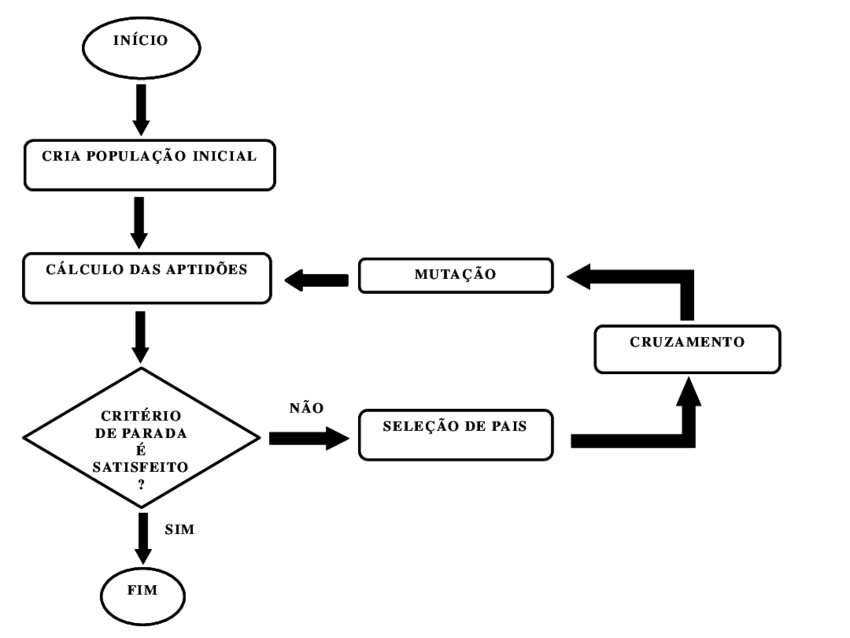
\includegraphics[width=1\textwidth]{cap_otimizacao-bio/figs/ga-flux.png}
	\caption{\label{fig_flux_ga}Fluxograma de um AG. Retirado de \cite{FiguraGA}}
\end{figure}

\begin{enumerate}  
	\item Sortear os pares de pais; 
	\item Aplicar o cruzamento em cada par e gerar os filhos; 
	\item Aplicar a mutação aos filhos, de acordo com uma taxa de mutação pré-estabelecida;
	\item Avaliar os filhos;
	\item Selecionar entre pais e filhos quais indivíduos formarão a população da iteração seguinte (reinserção).
\end{enumerate}

A evolução das gerações do AG termina quando uma condição de término estabelecida pelo usuário é atingida, por exemplo, encontrar a solução ótima do problema (quando conhecida) ou atingir um número máximo de gerações. Cada etapa de execução do AG é descrita com mais detalhes a seguir.

\subsection{Representação do indivíduo}
A principal dificuldade ao se elaborar um algoritmo genético é definir a representação do indivíduo. Cada indivíduo representa uma possível solução para o problema investigado e deve ser codificado em uma estrutura que possibilite e/ou favoreça a realização das operações genéticas de mutação e cruzamento. Na proposição original do AG \cite{Goldberg1989}, o indivíduo é representado de forma binária, ou seja, a solução para o problema é codificada em uma cadeia de bits, na qual cada posição pode facilmente ser invertida (mutação) ou copiada de um cromossomo para outro (cruzamento).

No problema da mochila 0/1, por exemplo, existe um conjunto de itens $I$ com pesos e valores e uma mochila com capacidade limitada. Deve-se descobrir qual a melhor forma de se arranjar os itens de maneira que a soma dos valores de cada um seja máxima e que a capacidade da mochila não seja excedida. Para representar uma solução deste problema em um AG, basta assumir um vetor binário de tamanho igual a $|I|$, onde diz-se que o item está na mochila se sua posição correspondente no vetor binário é 1 e não está, caso contrário.

Outras representações de indivíduos também são possíveis, mas apresentam novos desafios. Por exemplo, em problemas de menores caminhos, normalmente trabalha-se com árvores e caminhos. No PRM, o indivíduo é uma árvore e tanto a mutação quanto o cruzamento devem ser operações em árvores.

Para elaborar a representação do indivíduo no AG, deve-se levar em consideração a facilidade de manipulação da estrutura, a possibilidade de se introduzir um fator aleatório (mutação) e, principalmente, a representação das características de ambos os pais nos filhos. Se a estrutura não permite a herança de características, não é uma boa escolha para se utilizar em um algoritmo genético. Além disso, é preciso garantir a unicidade da forma de representação, ou seja, cada solução pode ser representada de uma única maneira e cada indivíduo deve representar uma única solução (relação um-para-um).

\subsection{Seleção de pais}
A estratégia para selecionar os pais que contribuirão para a composição genética da geração seguinte do AG deve ser escolhida de acordo com o propósito do algoritmo. Dependendo do problema, pode ser mais desejável uma convergência rápida que uma exploração mais profunda do espaço de busca, por exemplo. Os três métodos abaixo estão entre os mais empregados na etapa de seleção.

\begin{enumerate}
	\item Seleção elitista: os $t_e\%$ indivíduos da população com melhor aptidão formam um grupo de onde se sorteiam todos os pares de pais necessários para gerar a população de filhos. $t_e$ representa a taxa de elitismo, que é um parâmetro do AG. Dessa forma, não há chance de indivíduos muito ruins propagarem suas características. Portanto, a população converge para indivíduos iguais (ou muito parecidos) rapidamente, sem explorar partes do espaço de busca aparentemente ruins. Isso pode prejudicar o algoritmo em problemas com muitos mínimos locais, onde o fato de existir uma solução ruim não quer dizer que as soluções próximas também o são.
	\item Roleta: é um método menos rigoroso que o anterior. Cada indivíduo recebe uma probabilidade de ser selecionado de acordo com sua aptidão. Os indivíduos com maior aptidão receberão probabilidade alta e dificilmente não serão selecionados, enquanto indivíduos muito ruins raramente se tornarão pais. Apesar disso, toda solução tem chance de ser escolhida, o que melhora a exploração do espaço de busca em relação a estratégia anterior, mas pode diminuir a velocidade de convergência. Esta estratégia é um meio-termo entre a seleção elitista e a seleção por torneio, explicada a seguir.
	\item Seleção por torneio: esta é a estratégia com a menor pressão seletiva dentre os três métodos, ou seja, aquele que dá a maior chance aos indivíduos ruins de se tornarem pais e propagarem suas características. O torneio consiste em selecionar dois indivíduos aleatoriamente e escolher como primeiro pai aquele com a melhor aptidão, da mesma forma, sorteia-se dois outros indivíduos na população, diferentes do primeiro pai, e define-se como segundo pai a solução com melhor aptidão. O torneio básico é o torneio de dois, mas para aumentar a pressão seletiva, é possível realizar o torneio com um maior número de representantes da população. Dentre as três estratégias, esta é a que melhor explora o espaço de busca. Por outro lado, é possível que, ao explorar demasiadamente o espaço, o AG não consiga convergir.
\end{enumerate}

\subsection{Operadores genéticos}
Nos algoritmos genéticos, destacam-se duas operações principais que atuam sobre o código do indivíduo: cruzamento e mutação. O cruzamento e a mutação estão diretamente ligados com a forma de representação do indivíduo.

Num algoritmo genético, cada iteração do laço principal é chamada de geração. No início de cada geração, sorteia-se pares de pais de acordo com suas aptidões para que seja gerada uma nova população de filhos. A quantidade de pares de pais sorteados é determinada pela taxa de crossover, a qual é um parâmetro de configuração do AG. Cada par é composto de duas cadeias genéticas (cromossomos), uma correspondente a cada indivíduo do par. Para gerar o filho, cruza-se os dois cromossomos a fim de se obter dois novos indivíduos que compartilhem características de ambos genitores. Esse processo é conhecido como cruzamento, ou \textit{crossover}. Existem várias maneiras de se cruzar cadeias genéticas. A escolha depende principalmente da estrutura de dados usada para representar o cromossomo. A estrutura mais comum é a cadeia binária \cite{Goldberg1989}, onde uma solução é codificada em uma cadeia de 0's e 1's. Nesse caso, a forma mais simples de efetuar o cruzamento é gerar duas novas cadeias de bits (filhos), onde parte do material genético (posições na cadeia) pertence a um pai e o restante do material é proveniente do outro. Os filhos gerados em um cruzamento adotam materiais genéticos complementares de cada pai. Por exemplo, se o filho 1 herda os n primeiros genes do pai 1 e o restante do pai 2, o filho 2 herdará os $n$ primeiros genes do pai 2 e o restante do pai 1. A \autoref{fig_cross_ponto_unico} ilustra este tipo de cruzamento. Existem diversas formas de se combinar duas cadeias de bits, dentre elas podem-se destacar:

\begin{itemize}  
	\item Ponto de cruzamento único: uma posição $i$ de uma das cadeias é sorteada. O filho 1 herda os $i$ primeiros genes do pai 1 e restante do pai 2, enquanto que o filho 2 adota o material genético complementar. Na \autoref{fig_cross_ponto_unico}, é ilustrado um exemplo onde o ponto de cruzamento é estabelecido na metade.
	\item Dois pontos de cruzamento: ao invés de se utilizar apenas um ponto para dividir o material genético, este método divide a cadeia binária em três partes. Nesse caso, um filho herda a primeira e terceira partes de um pai e a segunda do outro.
	\item Cruzamento uniforme: cada bit do filho é obtido de forma aleatória, pode vir tanto do pai 1 quanto do pai 2. Em termos de implementação, sorteia-se uma máscara binária e para cada bit 0 da máscara, copia-se o gene do pai 1 para o filho. Para cada bit 1, copia-se o gene do pai 2.
	\item Cruzamento aritmético: realiza-se uma operação binária (ex: AND, OR, XOR, etc.) entre os cromossomos do pai 1 e do pai 2.
\end{itemize}

\begin{figure}[!htbp]
	\centering
	\renewcommand{\arraystretch}{2} 
	\begin{tabular}{rl}
		Pai 1: & 
		\renewcommand{\arraystretch}{1.15} 
		\begin{tabular}{|c|c|c|c|c|c|}
			\hline 
			\rowcolor[HTML]{F5D1CF}
			0 & 0 & 1 & 0 & 1 & 1 \\
			\hline 
		\end{tabular}
		\\
		Pai 2: & 
		\renewcommand{\arraystretch}{1.15} 
		\begin{tabular}{|c|c|c|c|c|c|}
			\hline 
			\rowcolor[HTML]{CCCCFF}
			1 & 0 & 0 & 1 & 1 & 0 \\
			\hline 
		\end{tabular}
		\\
		Filho 1: & 
		\renewcommand{\arraystretch}{1.15} 
		\begin{tabular}{|c|c|c|c|c|c|}
			\hline 
			\cellcolor[HTML]{F5D1CF}0 & \cellcolor[HTML]{F5D1CF}0 & \cellcolor[HTML]{F5D1CF}1 & \cellcolor[HTML]{CCCCFF}1 & \cellcolor[HTML]{CCCCFF}1 & \cellcolor[HTML]{CCCCFF}0 \\
			\hline 
		\end{tabular}
		\\
		Filho 2: & 
		\renewcommand{\arraystretch}{1.15} 
		\begin{tabular}{|c|c|c|c|c|c|}
			\hline 
			\cellcolor[HTML]{CCCCFF}1 & \cellcolor[HTML]{CCCCFF}0 & \cellcolor[HTML]{CCCCFF}0 & \cellcolor[HTML]{F5D1CF}0 & \cellcolor[HTML]{F5D1CF}1 & \cellcolor[HTML]{F5D1CF}1 \\
			\hline 
		\end{tabular}
	\end{tabular}
	\caption{\label{fig_cross_ponto_unico}Exemplo de \textit{crossover} com cruzamento de ponto único, onde o ponto de cruzamento está na metade do material genético.}
\end{figure}

A fim de melhorar a diversidade entre as soluções avaliadas, uma pertubação nos genes dos indivíduos é gerada durante a busca, possibilitando a exploração de elementos ausentes na população atual. Para isso, após gerar o cromossomo de cada filho, é preciso permitir que ocorra uma mutação, ou seja, uma mudança aleatória no material genético. A chance de uma mutação ocorrer depende de um parâmetro do AG chamado de ``taxa de mutação''. O processo de alteração genética aleatória depende da representação do indivíduo. No caso de uma cadeia binária, por exemplo, é simples, basta sortear um bit e invertê-lo. Em árvores, a mutação pode consistir na eliminação de algum vértice e na reconexão aleatória. Em grafos ponderados, alterar os pesos de uma aresta pode ser uma boa ideia. A definição do processo de mutação dependerá do problema e pode ser feita de várias maneiras diferentes, desde que produza uma pequena diferença no indivíduo e que ele continue representando uma solução válida.

O cruzamento normalmente gera um ou dois filhos para cada pai. Em todos os métodos descritos anteriormente é possível obter um segundo filho com o material genético não utilizado.

\subsection{Reinserção da População}
Independente do número de filhos gerados, após os processos de \textit{crossover} e mutação, a população será maior que o limite máximo permitido, exigindo a eliminação de alguns indivíduos (seleção natural). A reinserção opera sobre a aptidão (função de avaliação ou \textit{fitness}) de cada indivíduo da população. Diversas estratégias podem ser aplicadas nesse processo de seleção, também conhecido como reinserção. Por exemplo, a seleção natural sem elitismo, simplesmente elimina a população mais velha (pais). A seleção natural com elitismo mantém um percentual da população de pais (elite), completando-a com os melhores filhos. Outro tipo de elitismo é a seleção dos melhores indivíduos. Essa estratégia é normalmente mais interessante, pois permite a sobrevivência dos indivíduos mais aptos considerando a totalidade da população, sendo assim, avalia-se todos os pais e filhos e mantém-se aqueles com melhor aptidão.

\section{Otimização por Colônia de formigas}
\label{section_aco}
A otimização por colônia de formigas (ACO), proposto em \cite{Dorigo1996}, é um modelo de busca bio-inspirado que parte da ideia de que estruturas simples, com alguma espécie de comunicação, podem gerar um comportamento complexo quando operam em conjunto, de forma cooperativa. A inspiração do ACO é o forrageamento em uma colônia de formigas. Na natureza, observa-se que as formigas, mesmo sendo seres vivos simples, conseguem encontrar o melhor caminho entre o formigueiro e a fonte de comida. A partir do estudo desse comportamento, descobriu-se que tal faceta é possível através de uma comunicação indireta entre os animais. Ao fazer um caminho, as formigas depositam uma substância chamada feromônio, a qual pode ser percebida por outros membros da espécie. Uma formiga ao decidir qual caminho percorrer, tem maior chance de escolher aquele com a maior quantidade de feromônios. Além disso, a substância evapora com o tempo. Dessa forma, quanto menor o caminho, maior a frequência com a qual as formigas depositarão feromônio e, portanto, maior será a chance de ser escolhido.

Ao trazer o conceito de colônia de formigas para a computação, observa-se um grande potencial para se resolver problemas em grafo. Por exemplo, para descobrir o menor caminho entre os vértices $A$ e $B$ em um grafo não ponderado $G$, basta simular várias formigas que partem de $A$ e chegam em $B$, fazendo um caminho baseado na quantidade de feromônios das arestas. Ao final de cada iteração, atualiza-se o valor do feromônio em cada aresta de acordo com a evaporação e com as arestas percorridas pelas formigas. Dessa forma, espera-se que, após várias iterações, a quantidade de feromônios seja suficiente para guiar uma formiga pelo melhor caminho entre $A$ e $B$. O fluxograma de um ACO é mostrado na \autoref{fig_flux_aco}.

\begin{figure}[!htbp]
	\centering
	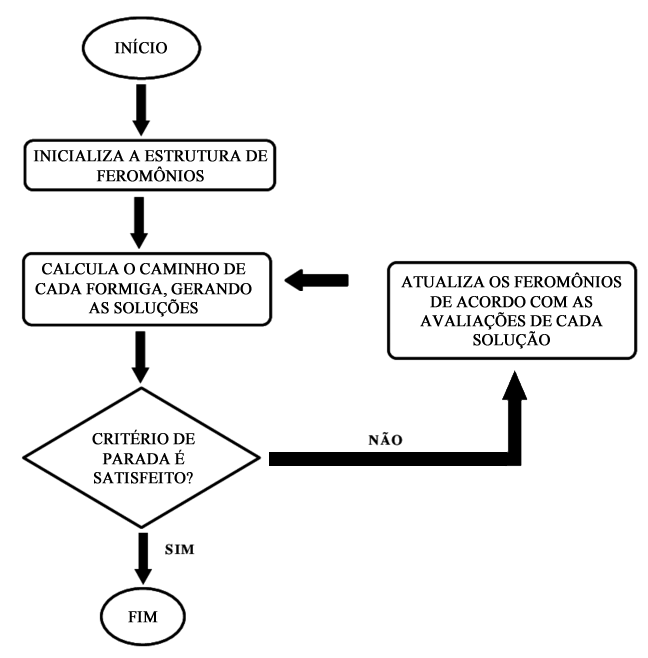
\includegraphics[width=0.7\textwidth]{cap_otimizacao-bio/figs/aco-flux.png}
	\caption{\label{fig_flux_aco}Fluxograma de um ACO.}
\end{figure}

O algoritmo inicia com a limpeza dos feromônios das arestas, ou seja, é atribuído zero para a quantidade de feromônio depositado em cada aresta do grafo. Após essa limpeza, inicia-se o processo iterativo do algoritmo onde, a cada iteração, as formigas na colônia percorrem o caminho do vértice de partida (formigueiro) ao nó destino (fonte de comida). Dependendo da formulação do problema, o caminho de volta também pode ser realizado. Ao final de cada iteração, atualiza-se os feromônios em cada aresta. O algoritmo termina quando uma condição de parada pré-determinada é atingida, normalmente um número máximo de iterações. As etapas principais da execução de um ACO são descritas a seguir.

\FloatBarrier
\subsection{Representação da solução}
No ACO, a solução é representada pelo caminho feito pela formiga no grafo, normalmente uma lista de vértices, uma árvore ou um subgrafo do grafo de entrada. Por exemplo, no problema de encontrar o menor caminho, a solução pode ser uma lista de vértices que representa o percurso desse caminho. Caso seja necessário encontrar caminhos entre a raiz e diversos destinos, pode-se representar a solução como uma árvore. Nem sempre é fácil decidir a codificação de uma solução. No problema da mochila, por exemplo, não é trivial a visualização de um grafo no processo da construção da solução. Nesse caso, uma possível representação é a associação de feromônios diretamente aos itens, através de um vetor de feromônios ao invés de uma matriz.

\subsection{Construção da solução} \label{section_construcao_solucao}
\label{section_otimizacao_aco_construcao}
Independentemente da representação escolhida, deve ser possível relacionar cada parte da solução com uma quantidade de feromônios na estrutura principal. Por exemplo, no caso de grafos, as arestas escolhidas para montar a solução devem ter seus feromônios incrementados a fim de guiar as próximas formigas. Em cada época (iteração do algoritmo) um número pré-determinado de soluções é construído, onde cada formiga decide quais partes serão adotadas em sua solução, com base nos respectivos valores de feromônios.

Além dos feromônios, as formigas ainda utilizam as informações de heurística para decidir o próximo passo. Uma heurística é uma função que estima a qualidade do caminho e normalmente representa o peso de uma aresta. Estando em um vértice $i$ de um grafo $G$, uma formiga tem probabilidade $p(i,j)$ de escolher a aresta que leva ao vértice adjacente $j$. Essa probabilidade é calculada pela seguinte equação:

\[ p(i,j) = \frac{\tau_{i,j}^\alpha * \eta_{i,j}^\beta}{\sum_{v \in adj(i)} \tau_{i,v}^\alpha * \eta_{i,v}^\beta} \]

Sendo:

\begin{itemize}  
	\item $\tau_{i,j}^\alpha$: feromônio na aresta $(i,j)$ elevado à constante $\alpha$, que representa a importância atribuída ao valor do feromônio. Representa o conhecimento sobre o ambiente (busca global).
	\item $\eta_{i,j}^\beta$: heurística da aresta $(i,j)$ elevada à constante $\beta$, que representa a importância atribuída à heurística. A heurística de uma aresta é dada em função do peso, como, por exemplo, $1/peso$, normalmente usado em problemas de minimização. Representa a visibilidade da formiga (busca local).
	\item $adj(i)$: são todos os vértices adjacentes a $i$, ou seja, todo vértice em $G$ para o qual é possível construir um caminho a partir de $i$ com apenas uma aresta.
\end{itemize}

O número de iterações (épocas), a quantidade de soluções geradas por iteração e as constantes alfa e beta são parâmetros de configuração de um algoritmo ACO. De forma geral, dado um grafo $G$ e um nó inicial, o processo de construção da solução sempre verifica todos os movimentos possíveis para a formiga, tomando sua decisão de acordo com os feromônios e as heurísticas de cada uma das possibilidades.

\subsection{Atualização dos feromônios}
Existem duas ocasiões onde o feromônio de uma aresta pode ser atualizado: no momento em que a formiga passa pela aresta e no fim de cada iteração. A maioria das implementações considera apenas o segundo caso, pois assim, é possível avaliar as soluções e incrementar os feromônios de acordo com os desempenhos obtidos. Ao fim de cada época, a quantidade de feromônio existente na aresta que liga os vértices i e j ($\tau_{i,j}$) é atualizada por:

\[ \tau_{i,j} = (1 - \rho) * \tau_{i,j} + \sum_{k \in formigas} \Delta\tau_{i,j}(k)\]

Sendo:

\begin{itemize}  
	\item $\rho$: parâmetro de configuração do ACO que corresponde ao coeficiente de evaporação. Determina o quão rápido o feromônio deve desaparecer das arestas após depositado.
	\item $formigas$: conjunto de todas as formigas na iteração.
	\item $\Delta\tau_{i,j}(k)$: quantidade de feromônio depositada pela formiga $k$ na aresta entre os vértices $i$ e $j$.
\end{itemize}

A quantidade de feromônio depositada por uma formiga $k$ em uma aresta entre os vértices $i$ e $j$ é dada por:

\[ \Delta\tau_{i,j}(k) = \begin{cases} \frac{Q}{L_k},& \text{se } x\geq 1\\ 0,& \text{caso contrário} \end{cases} \]

Sendo:

\begin{itemize}  
	\item $Q$: Quantidade máxima de feromônio que pode ser depositada por uma formiga.
	\item $L_k$: Custo da solução gerada pela formiga  $k$.
\end{itemize}

Considerando essas características, nossa pesquisa propõe uma nova versão de ACO para tratar problemas discretos com enfoque em otimização multiobjetivo.


% ----------------------------------------------------------
% Otimização multiobjetivo
% ----------------------------------------------------------
\chapter[Otimização multiobjetivo]{Otimização multiobjetivo}

A otimização multiobjetivo consiste em selecionar as melhores soluções de acordo com múltiplos critérios ao invés de apenas um. Por exemplo, ao estabelecer um melhor caminho entre duas cidades pode-se não estar interessado apenas na menor distância, mas também no tráfego, segurança das vias, quantidade de pedágios, etc. A otimização de apenas um objetivo é simples, para que uma solução seja considerada melhor que a outra, basta que ela tenha uma melhor avaliação. Por outro lado, quando se trabalha com mais de uma função de otimização, é preciso usar o conceito de dominância de Pareto.

A dominância de Pareto diz que uma solução $A$ é melhor que uma solução $B$, ou $A$ domina $B$ ($A \prec B$), se, e somente se:

\begin{itemize}  
	\item $A$ é melhor avaliado que $B$ em pelo menos um dos objetivos;
	\item $A$ não tem avaliação pior que $B$ em nenhum dos objetivos.
\end{itemize}

Considerando um problema de minimização e $F$ como o conjunto de funções objetivo, tem-se, matematicamente:

\[A \prec B \Leftrightarrow (\forall(f \in F) f(A) \leq f(B)) \land (\exists (f \in F) f(A) < f(B))\]

Em problemas de otimização multiobjetivo, o interesse está em encontrar o conjunto de todas as soluções que não são dominadas por nenhuma outra, ou seja, a fronteira de Pareto. Graficamente, a fronteira de Pareto representa a linha formada pelas soluções não-dominadas existentes para o problema. Na figura \ref{fig_pareto} apresenta-se um exemplo de uma fronteira de Pareto para um problema de minimização com dois objetivos ($F1$ e $F2$), a fronteira de Pareto está representada em vermelho. Observe que nenhum círculo vermelho possui ambos F1 e F2 menores que alguma outra solução em vermelho, ou seja, são não-dominadas. Em contra-partida, toda solução acima da fronteira, em cinza, é dominada, pois existe alguma solução em vermelho que possui ambos valores de F1 e F2 menores. Caso o problema em questão fosse de maximização, a fronteira de Pareto estaria acima de qualquer solução não-dominada ao invés de abaixo.

\begin{figure}
	\label{fig_pareto}
	\caption{Fronteira de Pareto}
	\centering
	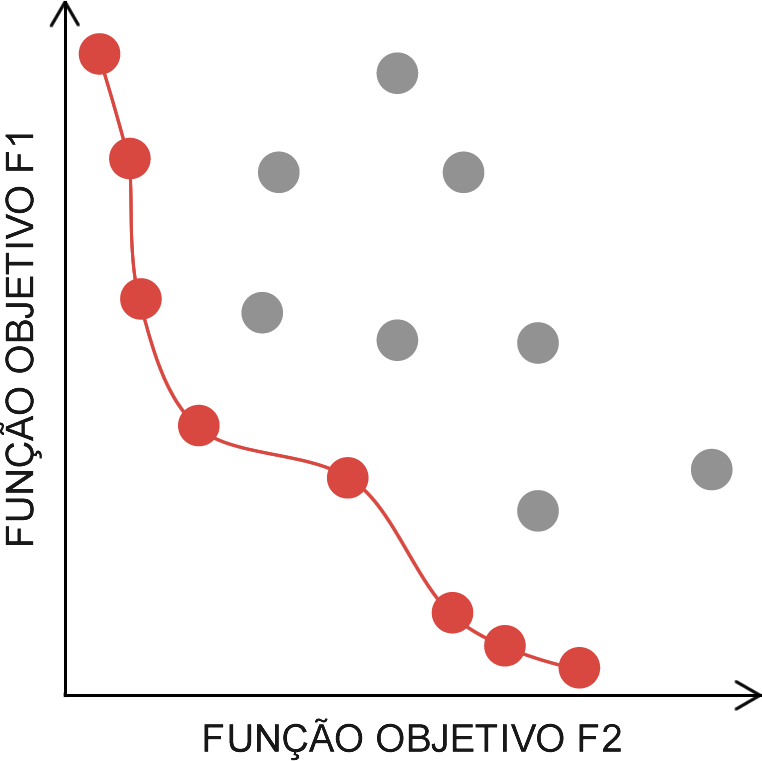
\includegraphics[width=0.4\textwidth]{cap_otimizacao-multi/figs/pareto}
\end{figure}

Não existe limite para o número de funções objetivo em um problema de otimização, mas quanto maior a quantidade de objetivos, mais complexa é a busca. Os algoritmos clássicos de otimização multiobjetivo NSGA-II e SPEA2 lidam bem com até três objetivos, mas a partir de quatro critérios de otimização, ambos os métodos sofrem para encontrar soluções relevantes. Desta forma, criou-se a classificação ``\textit{many-objective}''. Problemas \textit{many-objectives} (4 ou mais objetivos) apresentam diversas novas dificuldades e precisam de novas técnicas para que sejam resolvidos eficientemente. Como observado por Deb em \cite{Deb2014}, os problemas trazidos pelo alto número de objetivos são:

\begin{enumerate}  
	\item Grande parte da população é não dominada: a maioria dos algoritmos multiobjetivos classifica a população de acordo com a dominação de Pareto. Se existem muitas funções objetivo, se torna muito comum que uma solução seja melhor que outra em pelo menos uma das funções. Desta forma, a maior parte das soluções se torna não-dominada, o que impede os algoritmos de evoluírem a população, já que todos os indivíduos são considerados igualmente bons.
	\item Avaliar a diversidade da população se torna computacionalmente caro: afim de garantir uma boa diversidade populacional, alguns algoritmos medem alguma espécie de distância entre as soluções e removem as que são consideradas mais similares. A maior dimensionalidade traz consequentemente um maior impacto no cálculo da proximidade entre os indivíduos. 
	\item \textit{Crossover} ineficiente: a alta dimensionalidade do espaço de busca faz com que os indivíduos na população sejam muito distante uns dos outros e, normalmente, o cruzamento entre duas soluções muito diferentes resultam num filho muito distante dos pais, o que prejudica a convergência da busca. Portanto, pode ser necessário redefinir os operadores de recombinação afim de restringir as possibilidades de pareamento.
	\item População demasiadamente grande: quanto maior o número de objetivos, maior o número de soluções na fronteira de Pareto, portanto, para se obter bons resultados, é necessário que se manipule grandes populações de indivíduos, o que é computacionalmente caro e dificulta o trabalho do usuário que deverá escolher uma única solução ao final do processo.
	\item Métricas de avaliação se tornam difíceis de se calcular: a avaliação das soluções está diretamente relacionada ao número de objetivos, quanto maior ele for, maior será o esforço computacional necessário. A complexidade do hiper-volume, por exemplo, cresce exponencialmente com o número de objetivos.
	\item Dificuldade de visualização: é fácil representar graficamente as soluções e a fronteira de Pareto em problemas de até três objetivos. Com 4 funções em diante, se torna difícil tal visualização.
\end{enumerate}

A maior parte dos algoritmos many-objectives (todos mencionados neste trabalho) lidam apenas com os quatro primeiros problemas. As duas últimas não são responsabilidade dos algoritmos de otimização em sí.

\section{Algoritmos Multiobjetivo}

\subsection{Non-dominated Sorting Genetic Algorithm II (NSGA-II)}
O NSGA-II \cite{Deb2002} é o algoritmo evolutivo multiobjetivo (AEMO) mais frequente na literatura. A atribuição de aptidão (\textit{fitness}) se dá pela classificação da população em rankings de dominância (fronteiras), de forma que o primeiro contenha todas as soluções não dominadas, o segundo todos os indivíduos não-dominados excluindo a primeira fronteira, e assim por diante. Quanto melhor o \textit{ranking} de uma solução, melhor sua aptidão e  maior sua chance de sobreviver para a próxima geração. Várias soluções, pertencem à mesma fronteira, a fim de diferenciá-las utiliza-se um cálculo de distância (\textit{crowding distance}), o qual confere melhor avaliação às soluções mais diferenciadas umas das outras, garantindo assim a diversidade da população.

O processo do NSGA-II é semelhante ao do algoritmo genético comum, com diferença no cálculo de aptidão, que é feito por \textit{ranks}, e no cálculo de distâncias, que é inexistente na proposta original do AG. O primeiro passo continua sendo a geração aleatória dos indivíduos, em seguida classifica-se a população em \textit{ranks} de dominância e inicia-se o laço principal, o qual termina assim que a condição de parada é atingida. O laço principal do NSGA-II é dado pelo pseudo-código do algoritmo \ref{alg_nsgaii}.

\begin{algorithm}
	\caption{Laço principal do NSGA-II}
	\label{alg_nsgaii}
	\begin{algorithmic}[1]
		\While {número máximo de gerações não for atingido}
		\State selecione os pares de pais para o crossover
		\State efetue o cruzamento para cada par de pais, gerando os filhos
		\State combine a população de pais com a população de filhos
		\State classifique todas as soluções em fronteiras (\textit{ranks}) de dominância 
		\State calcule a \textit{crowding distance} para cada uma das soluções
		\State aplique a seleção natural sobre a totalidade da população, preservando os indivíduos de melhor \textit{rank} e, em segundo lugar, \textit{crowding distance}.
		\EndWhile
	\end{algorithmic}
\end{algorithm}

A seleção de pais utiliza torneio simples para o sorteio, ou seja, dois elementos da população são escolhidos de forma aleatória, o indivíduo com melhor avaliação é selecionado como um dos pais, sorteia-se mais dois indivíduos, e o melhor dentre eles se torna o segundo pai.

Na linha 2 do pseudo-código, através dos pares de pais, gera-se os filhos com o \textit{crossover} e a mutação. Após a geração dos filhos, a população corrente e o conjunto de filhos são concatenados (linha 3) e submetidos à classificação em \textit{ranks} de dominância (linha 4).

A classificação em \textit{ranks} de dominância recebe um conjunto de soluções e verifica quais dentre elas não são dominadas. O conjunto de soluções não-dominadas forma o primeiro \textit{rank} de dominância. Do conjunto restante (excluindo o primeiro \textit{rank}), retira-se as soluções não dominadas para formar o segundo \textit{rank}. Esse processo se repete até que todos os indivíduos tenham sido classificados.

Após toda a população ter sido classificada em \textit{ranks}, antes de selecionar os indivíduos que vão compor a população na próxima iteração, deve-se calcular a distância de aglomeração (\textit{crowding distance}) para cada indivíduo em cada \textit{rank} de dominância. O cálculo de distância, para cada objetivo, ordena o conjunto de soluções e faz uma relação entre as distâncias de cada indivíduo para os vizinhos imediatamente anterior e posterior. Soma-se as distâncias obtidas em cada objetivo para cada solução e define-se aquelas com maior valor de distância como as mais diferentes entre sí.

Com toda a população classificada em \textit{ranks} (ou fronteiras) e todas as distâncias calculadas, basta formar a nova população com os melhores indivíduos. Para isso, analisa-se fronteira a fronteira, da melhor para a pior, até que o tamanho máximo da população seja atingido. Para cada fronteira aplica-se o seguinte processo de decisão:

\begin{itemize}  
	\item Se $tamanho(rank) + tamanho(nova_população) < tam_max_pop$: adiciona-se todos os membros do \textit{rank} à nova população.
	\item Caso contrário, se $tamanho(nova_população) < tam_max_pop$: adiciona-se à nova população os $tam_max_pop - tamanho(nova_população)$ elementos do \textit{rank} com os maiores valores de distância. Termine o processo, a nova população está formada.
	\item Caso contrário, termine o processo, a nova população está formada.
\end{itemize}

Desta forma, ao final do algoritmo obtém-se a fronteira de Pareto aproximada na primeira fronteira da população gerada na última iteração do algoritmo.

\subsection{Strength Pareto evolutionary algorithm 2 (SPEA2)}

O SPEA2 \cite{Zitzler2002} é um AEMO que calcula, para cada membro da população, sua força (\textit{strength}) e densidade. A força de uma solução é dada pelo número de indivíduos que ela domina, enquanto a densidade é uma medida de distância para os vizinhos mais próximos, quanto maior a densidade mais próximo o indivíduo está das demais soluções. A aptidão (\textit{fitness}) de uma solução é definida por sua densidade mais a soma das forças de todo indivíduo que a domina. As principais diferenças entre o SPEA2 e um AG comum estão no cálculo de aptidão e na utilização de uma população extra: o arquivo.

O arquivo é responsável por guardar as melhores soluções já encontradas até o momento, funciona como uma espécie de elitismo. Os pais, no cruzamento, são sempre escolhidos do arquivo e os filhos substituem 100\% da população corrente. A cada iteração, os melhores indivíduos entre a população e o arquivo compõe o arquivo da geração seguinte. A quantidade de indivíduos no repositório de soluções não-dominadas é limitada e, portanto, quando se excede o tamanho máximo, deve-se executar um processo de truncamento.

O processo de truncamento do arquivo ocorre na seleção natural, a última função executada na iteração do laço principal de um AG. A seleção no SPEA2 se dá pelo cálculo do arquivo da próxima geração: ambas as populações da iteração corrente (população e arquivo) são submetidas à seleção, extrai-se do conjunto total de soluções aquelas que não são dominadas por nenhuma outra e com esse subconjunto ($n_d$) constrói-se o novo arquivo através do seguinte processo de decisão:

\begin{itemize}  
	\item Se $tamanho(n_d) = capacidade\_arquivo$, o novo arquivo é formado por $n_d$;
	\item Caso contrário, se $tamanho(n_d) < capacidade\_arquivo$, o novo arquivo é formado pela união de $n_d$ com os $capacidade\_arquivo - tamanho(n_d)$ indivíduos restantes com melhor aptidão;
	\item Caso contrário, se $tamanho(n_d) > capacidade\_arquivo$, o novo arquivo é formado por $n_d$ e deve-se truncá-lo em $tamanho(n_d) - capacidade\_arquivo$ passos, onde em cada passo elimina-se o indivíduo com menor variabilidade genética em relação aos demais.
\end{itemize}

Os indivíduos mais aptos no SPEA2 são aqueles dominados pela menor quantidade de soluções e que possuem maior variabilidade genética. O algoritmo calcula a aptidão em três etapas: cálculo de força (\textit{strength}), do \textit{raw fitness} e da densidade.

A força de um indivíduo $i$ ($s(i)$) é o número de soluções que ele domina, ou seja, considerando $A$ o arquivo e $P$ a população:

\[ s(i) = |j|: j \in P \cup A \land i \prec j \]

Tendo calculado a força de cada indivíduo, parte-se para o \textit{raw fitness}. O \textit{raw fitness} de um indivíduo $i$ ($r(i)$) é dado pela soma das forças de cada elemento que o domina. Veja a fórmula a seguir:

\[ r(i) = \sum_{j \in A \cup P | j \prec i} s(j) \]

Observe que, caso o indivíduo seja não-dominado, seu \textit{raw fitness} será o menor possível: zero. Após determinar o \textit{raw fitness}, para finalizar o cálculo de aptidão deve-se descobrir a densidade de cada indivíduo ($d(i)$). A densidade é computada de acordo com a distância da solução para seus vizinhos e é dada pela seguinte fórmula:

\[ d(i) = \frac{1}{\sigma_i^k + 2} \]

Na fórmula acima, $\sigma_i^k$ é a k-ésima menor distância entre o indivíduo $i$ e o restante da população. k é a raiz quadrada do tamanho do conjunto de soluções em avaliação, i.e. $k = \sqrt{|P \cup A|}$. O valor de $d(i)$ sempre está no intervalo (0,1). Referencia-se o leitor ao artigo original do SPEA2 \cite{Zitzler2002} para mais detalhes sobre o cálculo de densidade.

Finalmente, a aptidão do indivíduo ($f(i)$) é dada pela soma do \textit{raw fitness} e a densidade: $f(i) = r(i) + d(i)$. Note que, se a solução $i$ é não-dominada, $f(i) < 1$. isso acontece, pois $d(i) < 1$ para qualquer solução e quando $i$ é não-dominada, $r(i) = 0$.

O laço principal do SPEA2 é explicitado no pseudo-código \ref{alg_spea2} e como resposta para o problema, retorna-se o arquivo da última geração computada. Espera-se que, após as diversas iterações, o algoritmo tenha conseguido uma boa aproximação da fronteira de Pareto.

\begin{algorithm}
	\caption{Laço principal do SPEA2}
	\label{alg_spea2}
	\begin{algorithmic}[1]
		\While {número máximo de gerações não for atingido}
		\State a partir do arquivo, selecione os pares de pais para o crossover
		\State efetue o cruzamento para cada par de pais, gerando os filhos
		\State substitua a população corrente pelos filhos
		\State calcule o fitness de todos indivíduos no arquivo e na população
		\State aplique a seleção natural e trunque o arquivo, caso necessário
		\EndWhile
	\end{algorithmic}
\end{algorithm}

\section{Algoritmos Many-objectives}

\subsection{Multiobjective evolutionary algorithm based on decomposition (MOEA/D)}
\label{section_moead}

O MOEA/D \cite{Zhang2007} é um algoritmo que avalia os objetivos através de uma função escalarizadora, se baseando na dominância de Pareto apenas para atualizar o conjunto de soluções não dominadas geradas em cada iteração (arquivo). No MOEA/D, um problema multiobjetivo é decomposto em múltiplos problemas mono-objetivos chamados de células. Cada célula é definida por um vetor de pesos gerado aleatoriamente e representa um indivíduo, ou seja, o número de células é igual ao tamanho da população. Além dos pesos, a célula, ou indivíduo, é composta de uma solução e uma vizinhança. A vizinhança é formada pelos $k$ indivíduos mais próximos de acordo com o vetor de pesos, onde $k$ é um parâmetro do algoritmo que representa o tamanho das vizinhanças. A aptidão (\textit{fitness}) de uma solução é calculada de acordo com sua avaliação em cada objetivo, a função escalarizadora, e o vetor de pesos da célula. Em toda geração, uma nova solução é gerada para cada célula, onde a vizinhança é levada em consideração para a escolha dos pais e seleção natural.

O primeiro passo do MOEA/D é gerar a estrutura de células e vizinhanças, para isso, sorteia-se os vetores de pesos (a soma de cada vetor deve ser igual a um) e para cada um deles, calcula-se os $k$ vetores mais próximos (vizinhança). Essa estrutura é imutável e é utilizada no decorrer de todo o algoritmo. A geração dos vetores de pesos pode ser tanto aleatória quanto seguir uma distribuição pré-definida. Antes de começar o laço principal, gera-se aleatoriamente uma solução para cada célula e calcula-se as aptidões. 

Uma parte fundamental do MOEA/D é a escolha da função escalarizadora, ela é a principal responsável pelo cálculo de aptidão. Em todos experimentos realizados neste trabalho, foi utilizada a soma ponderada, mas outras estratégia como \textit{Penalty-Based Boundary Intersection} e Tchebycheff também podem ser utilizadas \cite{Zhang2007}. A aptidão de uma solução é calculada através da função escalarizadora e do vetor de pesos, por exemplo, se os valores $[2, 9, 5]$ representam a solução $s$ no espaço de objetivos, $[0.3, 0.2, 0.5]$ é o vetor de pesos da célula $c$, e a soma ponderada é a função escalarizadora, então a aptidão de $s$ em $c$ é dada por $2 * 0.3 + 9 * 0.2 + 5 * 0.5 = 4.9$.

No laço principal do MOEA/D, seleciona-se os pais e gera-se os filhos. Para cada célula $c_i$, dois pais são selecionados aleatoriamente em sua vizinhança. Sempre que um filho é gerado, o processo de seleção é realizado logo em seguida. A aptidão do filho é calculada para cada uma das células na vizinhança de $c_i$, substituindo a solução anterior de uma célula caso seu fitness seja melhor. Após o processo de geração de filhos e seleção, atualiza-se o arquivo com as novas soluções não-dominadas.

\subsection{Non-dominated Sorting Genetic Algorithm III (NSGA-III)}

O NSGA-III \cite{Deb2014} é uma extensão do NSGA-II que permite o \textit{framework} funcionar melhor para mais de três objetivos. Ele se diferencia do original apenas na fase de seleção, onde ao invés de usar a distância de aglomeração para diferenciar soluções em uma mesma fronteira, utiliza um método de clusterização, onde os indivíduos são divididos em nichos de acordo com suas similaridades. O NSGA-III é caracterizado pelo processo de atribuição de nicho chamado de classificação não-dominada baseada em pontos de referência. Sua ideia é traçar uma figura geométrica de uma dimensão a menos que o número de objetivos nos pontos extremos da primeira fronteira. Um número pré-definido de pontos de referência equidistantes é distribuído sobre a figura e passa a representar cada um, um nicho. Para classificar uma solução, define-se como nicho o ponto de referência mais próximo. Ao final, toma-se como sobreviventes os pontos nas regiões menos lotadas do espaço de busca. Para mais detalhes sobre o processo de clusterização, referencia-se o leitor ao artigo original [NSGA-III].

\subsection{SPEA2 with Shift-Based Density Estimation (SPEA2-SDE)}

O SPEA2-SDE \cite{Spea2SDE} é uma pequena alteração no algoritmo SPEA2 que o permite trabalhar com 4 ou mais objetivos de forma muito mais eficiente. A única alteração está no cálculo de distância entre duas soluções. Suponha que $s_1$ e $s_2$ sejam dois indivíduos na população e que seus valores no espaço de objetivo sejam, respectivamente, $[5, 10, 351, 7, 15]$ e $[6, 8, 15, 9, 14]$. No SPEA2, a distância entre $s_1$ e $s_2$ é dada pela distância euclidiana dos dois vetores, ou seja, $distancia(s_1, s_2) = \sqrt{(5-6)^2 + (10-8)^2 + (351-15)^2 + (7-9)^2 + (15-14)^2} = 336,0148$. As duas soluções são, na verdade bem próximas, pois só estão distantes em uma das 5 coordenadas, mas o cálculo de distância do SPEA2 não reflete isso, o que é prejudicial em problemas com muitos objetivos. A fim de resolver esse problema, Miqing Li et al. introduziram o cálculo de distância Shift-Based Density Estimation (SDE), que nada mais faz do que transladar a coordenada mais distante do segundo ponto para o mesmo valor no primeiro ponto, isto é, antes de calcular a distância euclidiana, identifica-se a coordenada que exibe maior diferença entre os dois pontos, no caso dos exemplos $s_1$ e $s_2$, a terceira coordenada é a que possui esse comportamento. Em seguida, modifica-se o segundo ponto na coordenada identificada para que seja igual ao primeiro ponto, no exemplo, cria-se $s_2' = [6, 8, 351, 7, 15]$. A distância SDE é então determinada pela distância euclidiana entre o primeiro ponto e o segundo ponto transladado. No exemplo, a distância final vale $distancia(s_1, s_2') = \sqrt{(5-6)^2 + (10-8)^2 + (351-351)^2 + (7-9)^2 + (15-14)^2} = 3,1622$. A distância SDE, em resumo, descarta a coordenada mais distante ao calcular as distâncias, permitindo assim que pontos distantes em apenas uma coordenada ainda sejam considerados próximos. Todo o restante do processo do SPEA2 segue da mesma maneira que o algoritmo original.

\subsection{Algoritmo Evolutivo Multiobjetivo com Muitas Tabelas (AEMMT)}

O AEMMT \cite{Brasil2013}, assim como o MOEA/D, decompõe o problema multiobjetivo em subproblemas menores e para isso utiliza um esquema de tabelas, onde cada tabela representa uma combinação diferente de objetivos. A função que transforma os múltiplos objetivos em um valor escalar é sempre a média e cada tabela mantém os melhores indivíduos considerando a média dos objetivos que representa. A cada geração, duas tabelas são selecionadas para o cruzamento. Dois pais, um de cada tabela, são sorteados aleatoriamente para gerarem um único filho, que será testado em todas as tabelas, entrando naquelas em que representar uma melhor aptidão em relação aos demais indivíduos. Naturalmente, como um único \textit{crossover} é realizado a cada iteração, o AEMMT precisa de mais gerações para efetuar o mesmo número de comparações que os algoritmos citados nas seções anteriores.

A quantidade de tabelas é determinada pelo número de combinações possíveis de objetivos. Para quatro objetivos ($f_1, f_2, f_3, f_4$), por exemplo, como ilustrado na figura \ref{fig_aemmt_tabelas} serão criadas 15 tabelas de combinações mais uma tabela extra, usada para guardar os indivíduos não-dominados.

\begin{figure}
	\label{fig_aemmt_tabelas}
	\caption{Tabelas do AEMMT}
	\centering
	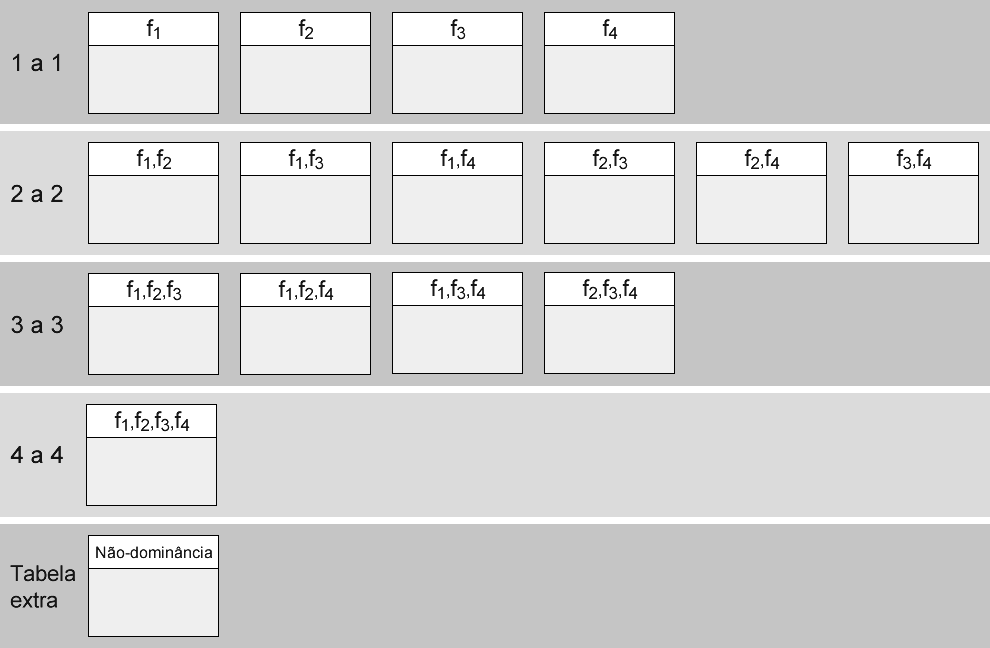
\includegraphics[width=1\textwidth]{cap_otimizacao-multi/figs/aeemt-tabelas}
\end{figure}

Cada tabela possui um limite máximo de indivíduos e no início do algoritmo gera-se soluções aleatórias de forma que todas as tabelas sejam completamente preenchidas. No laço principal, um indivíduo só entra em uma tabela $t$ se for melhor que a pior solução na população de $t$. Com relação a tabela de dominância, sempre que um filho é gerado e não-dominado por nenhum outro indivíduo na tabela, ele é incluído. A restrição no tamanho da tabela de dominância é independente das demais e sempre que o limite for atingido, é feito um truncamento priorizando a permanência das soluções com maior valor de média aritmética entre todos os objetivos.

O primeiro passo do AEMMT é gerar as tabelas e preenchê-las com soluções aleatórias. Em seguida, inicia-se o laço principal, onde em cada iteração são escolhidas duas tabelas via torneio duplo de acordo com suas pontuações. A pontuação tem valor inicial zero e sempre que uma tabela gera um filho que sobrevive para a geração seguinte, sua pontuação é incrementada. As pontuações são zeradas a cada 100 gerações. Considerando as duas tabelas que vencem os torneios, sorteia-se um indivíduo de cada e efetua-se o cruzamento entre os dois. O filho gerado é então comparado tabela à tabela, entrando naquelas em que representar uma melhoria. Após a execução de todas as gerações, dá-se como resultado o conjunto não dominado entre as soluções de todas as tabelas.

\subsection{Algoritmo Evolutivo Multiobjetivo com Múltiplas Dominâncias (AEMMD)}
\label{section_aemmd}

O AEMMD \cite{Lafeta2016}, é uma modificação do AEMMT que, apesar de usar o mesmo processo de divisão do problema multi-objetivo, abandona a ideia de escalarização e volta a utilizar o conceito de dominância dos métodos mais antigos (e.g. NSGA-II e SPEA2). No AEMMD, ao invés de se utilizar a média dos objetivos da tabela para avaliar o indivíduo, lança-se mão da relação de dominância de Pareto, um indivíduo novo $s$ só entra na tabela $t$, se $s$ não for dominado por nenhuma solução em $t$ considerando apenas os objetivos de $t$. Além disso, se $s$ entra em $t$, todas as soluções em $t$ dominadas por $s$ são removidas.

O primeiro passo do AEMMD é gerar o conjunto de tabelas, que é composto por todas as combinações de objetivos possíveis a partir de dois a dois. Combinações de um único objetivo não são criadas, pois o conceito de dominância é válido apenas para a partir de dois valores. Diferentemente do AEMMT, as tabelas não possuem limite de tamanho e podem crescer indefinidamente. Para um problema de quatro objetivos ($f_1, f_2, f_3, f_4$), por exemplo, 11 tabelas seriam geradas, veja a figura \ref{fig_aemmd_tabelas}.

\begin{figure}
	\label{fig_aemmd_tabelas}
	\caption{Tabelas do AEMMD}
	\centering
	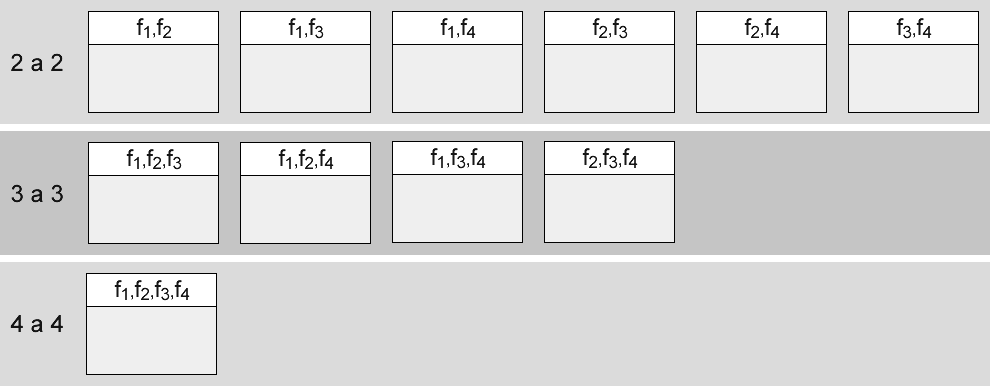
\includegraphics[width=1\textwidth]{cap_otimizacao-multi/figs/aeemd-tabelas}
\end{figure}

Com as tabelas criadas, gera-se um número pré-definido de soluções aleatórias, distribuindo-nas pelas tabelas de acordo com a relação de dominância de Pareto. O próximo passo é o laço principal, onde a cada iteração, através de um torneio duplo, sorteia-se duas tabelas de acordo com suas pontuações. A pontuação das tabelas no AEMMD é diferente do AEMMT, ao invés de conceder um ponto sempre que se gera um indivíduo sobrevivente, pontua-se uma tabela quando ela recebe um indivíduo. Tendo escolhido as duas populações pais, sorteia-se um representante de cada e gera-se um único filho, o qual é comparado tabela à tabela e entra naquelas onde representa uma solução não dominada. Outra diferença em relação ao método original, é que o AEMMD não reinicia as pontuações em momento algum do algoritmo. Espera-se que ao final das gerações, a população da tabela principal, com todos os objetivos, tenha convergido para a fronteira de Pareto. 

\section{Algoritmos many-objectives baseados em colônias de formigas}

A maior parte dos métodos de busca multiobjetivo são baseados em algoritmos genéticos, mas uma boa alternativa pouco explorada é a inteligência coletiva, representada por estratégias como as colônias de formigas (ACOs) e enxame de partículas (PSOs). Neste trabalho, devido ao fato de explorar-se dois problemas discretos (problema da mochila multiobjetivo e problema do roteamento multicast), optou-se por utilizar as colônias de formigas, que foram desenvolvidas especialmente para lidar com esse tipo de problema. Como explicado em [secao\_formigas], ao invés de utilizarem os operadores genéticos para gerarem e evoluírem a população, os ACOs lançam mão de um processo de construção de solução baseado em feromônios, o qual decide, a cada passo, uma partícula da solução de acordo seu valor de feromônio e heurística. Dentre os ACOs multiobjetivos propostos na literatura, destacam-se o MOACS, ...

\subsection{Multi-Objective Ant Colony Optimization Algorithm (MOACS)}

O MOACS foi proposto pela primeira vez em \cite{Baran2003} para o problema de roteamento de veículos com janelas de tempo e posteriormente foi aplicado no problema do roteamento multicast \cite{Pinto2005}. A última versão do algoritmo foi proposta em \cite{Riveros2016} e essa é a variação utilizada neste trabalho. O MOACS é uma adaptação do ACO original que torna possível a otimização de múltiplos objetivos utilizando uma única estrutura de feromônios, múltiplas heurísticas e um arquivo de soluções não dominadas. Veja o código do algoritmo \ref{alg_moacs}.

\begin{algorithm}
	\caption{Algoritmo MOACS}
	\label{alg_moacs}
	\begin{algorithmic}[1]
		\State Inicialize a estrutura de feromônios $\tau_{ij}$ com $\tau_0$ /* $\tau_{0}$ é o valor inicial */
		\State Crie um conjunto vazio de soluções não-dominadas $ND$
		\While {Número máximo de iterações não for atingido}
		\For {$i \gets 0$ até $tamanho\_populacao$}
		\State Sorteie valores no intervalo $[0, w_{max}[$ para formar um vetor de pesos $W$ com $|H|$ posições
		\State Construa uma solução de acordo com a tabela de feromônios $\tau_{ij}$, as heurísticas ($H$) e os pesos $W$
		\State Atualize $ND$ com a nova solução
		\EndFor
		\If {$ND$ foi modificado}
		\State Reinicie a estrutura de feromônios fazendo $\tau_{ij} = \tau_0 \forall(i,j)$
		\Else
		\State Atualize a estrutura de feromônios com todas as soluções em $ND$
		\EndIf
		\EndWhile
		\State \Return $ND$
	\end{algorithmic}
\end{algorithm}

O processo de construção da solução depende do problema e, no MOACS, os principais componentes para o processo são:

\begin{itemize}  
	\item Feromônios ($\tau_{ij}$): estrutura que guarda a quantidade de feromônios em cada partícula que pode formar a solução. No caso de problemas em grafos, representa a quantidade da substância em cada uma das arestas;
	\item Heurísticas ($H$): conjunto de funções que estimam a qualidade de uma dada partícula que pode formar a solução. No caso de problemas em grafos, representa os vários pesos em uma aresta. Por exemplo, num grafo que representa uma rede de computadores com informações de custo, distância e tráfego, $H$ poderia ser formado de três funções que recebem uma aresta $(i,j)$ e devolvem, respectivamente, os valores de peso, distância e tráfego na aresta.
	\item Peso máximo de uma heurística ($w_{max}$): representa o valor máximo que o peso de uma heurística pode atingir. Em \cite{Riveros2016}, propõe-se $w_{max} = 3$, de forma que cada função possa ser classificada como 0 (não importante), 1 (importante), 2 (muito importante).
	\item Vetor de pesos ($W$): O vetor de pesos atribui a importância de cada heurística e é gerado aleatoriamente em cada iteração. Cada função de heurística recebe um peso variando no intervalo $[0, w_{max}[$.
\end{itemize}

Ao construir uma solução, utiliza-se o mesmo processo de decisão do ACO original, explicado na seção \ref{section_construcao_solucao}. A única diferença é que as múltiplas heurísticas do MOACS ($H$) deve ser unificada em uma única função $h(x)$, para isso utiliza-se o vetor de pesos $W$ para se aplicar uma média ponderada. Veja a equação a seguir:

\[h(x) = \frac{\sum_{i \gets 0}^{size(H)}\ H_i(x) * W_i}{\sum_{w \in W} w}\]

Em cada época (iteração do laço principal), atualiza-se o arquivo de soluções não dominadas com as novas soluções geradas. Se o arquivo foi atualizado após criar-se todas as soluções, reinicia-se as informações de feromônio, redefinindo todos os valores na estrutura $\tau_{ij}$ para o valor inicial de feromônio $\tau_0$. Caso o arquivo tenha se mantido estável, ou seja, nenhuma das novas soluções seja não-dominada, atualiza-se as quantidades de feromônio na estrutura de acordo com as soluções no arquivo.

Considerando um problema em grafos, para atualizar a estrutura $\tau_{ij}$ com uma solução $s$, faz-se:

\[\tau_{ij} = (1 - \rho) * \tau_{ij} + \rho * \Delta\tau(s) \forall(i,j) \in s\]

Onde:
\begin{itemize} 
	\item $\rho$: coeficiente de evaporação;
	\item $\Delta\tau(s)$: Quantidade de feromônios depositados pela solução $s$.
\end{itemize}

A quantidade de feromônio depositado pela solução $s$ ($\Delta\tau(s)$) é definida por:

\[\Delta\tau(s) = \frac{1}{performance(s)}\]

Na fórmula anterior, $performance(s)$, é dado pela soma dos valores de $s$ no espaço de objetivos. Neste caso, considera-se um problema de minimização, para problemas de maximização, basta inverter a equação. Se os objetivos são reduzir o custo, o tráfego e o delay de uma rede, por exemplo, $performance(s) = custo(s) + trafego(s) + delay(s)$.

Após todas as iterações do laço principal, espera-se obter no arquivo uma boa aproximação da fronteira de Pareto. 

\subsection{Multiobjective evolutionary algorithm based on decomposition and ACO (MOEA/D-ACO)}
O MOEA/D-ACO [] é o algoritmo MOEA/D (seção \ref{section_moead}) aplicado ao \textit{framework} de otimização por colônia de formigas (ACO). Os conceitos de células e vizinhanças são reutilizados, enquanto que a reprodução local, inexistente no ACO, é substituída por um processo de construção da solução levemente modificado. Além disso introduz-se um novo conceito de grupos que é utilizado para \textit{clusterizar} as formigas de acordo com seus vetores de peso. Chama-se de formiga neste algoritmo o que era chamado de célula, no MOEA/D.

O primeiro passo do MOEA/D-ACO consiste em gerar os vetores de peso que, assim como no MOEA/D, são \textit{arrays} de valores entre 0 e 1 cujas somas valem 1. A geração pode ser aleatória ou seguir uma distribuição pré-definida. No caso deste trabalho, utilizou-se a distribuição uniforme proposta no artigo original []. Atribui-se cada vetor a uma formiga e cria-se a estrutura de vizinhanças, onde cada formiga é associada a uma vizinhança contendo as $v_size$ formigas mais próximas de acordo com os vetores de peso (incluindo ela mesma). O segundo passo do algoritmo determina os grupos, cada grupo recebe um novo vetor de pesos gerado da mesma maneira que os pesos anteriores. As formigas são então distribuídas entre os grupos de acordo com a proximidade entre seu vetor de pesos e o vetor de pesos do grupo (\textit{clusterização}).

Com respeito às duas principais estruturas de um ACO, heurística e feromônios, cada formiga possui uma função heurística e cada grupo mantem uma estrutura de feromônios. Quando os grupos são criados, cada um recebe uma estrutura de feromônios com o valor máximo de feromônio em cada uma das posições. A formiga, por sua vez, quando criada recebe uma função heurística baseada na combinação de todas as funções heurísticas do problema e no vetor de pesos da própria formiga. O cálculo específico da heurística depende do problema e será visto na seção \ref{section_estrategias_prm_aco} para o PRM e na seção \ref{section_estrategias_pmm_aco} para o PMM.

O laço principal do MOEA/D-ACO consiste em gerar as soluções, atualizar o conjunto de soluções não-dominadas $ND$, distribuir as novas soluções entre as formigas e atualizar as estruturas de feromônios. Primeiramente, para cada grupo $G$, gera-se as soluções para cada formiga $f \in G$. A solução é gerada com base nos feromônios de $G$, na heurística de $f$ e na solução atual de $f$. Tendo gerado todas as soluções para um grupo, atualiza-se o arquivo de soluções não-dominadas $ND$. Para cada nova solução que entrou no arquivo, modifica-se a estrutura de feromônios de $G$ de acordo com a fórmula a seguir:

[]

Cada formiga armazena duas soluções, a solução atual, que de início é nula, e a nova solução, criada em cada iteração do laço principal. Após passar por todos os grupos e suas formigas gerando as novas soluções e atualizando os feromônios, deve-se decidir a solução atual de cada formiga com base nas novas soluções da vizinhança, o que é feito da seguinte maneira: para cada formiga $f$, analisa-se as novas soluções presentes na vizinhança de $f$; se alguma nova solução $ns$ que ainda não substituiu nenhuma outra possui um \textit{fitness} melhor que o da solução corrente de $f$ ($sc$), substitui-se $sc$ por $ns$. O \textit{fitness} é calculado de acordo com a média pondera dos valores da solução em cada objetivo baseadas no vetor de pesos da formiga em questão. Neste trabalho utilizou-se a soma ponderada como função \textit{escalarizadora}, mas qualquer uma das funções propostas em \cite{Zhang2007} poderia ter sido usada.

O processo de construção da solução depende do problema e é apresentado nas seções \ref{section_estrategias_prm_aco} para o PRM e  \ref{section_estrategias_pmm_aco} para o PMM. Mas, de qualquer forma, independente do problema, o MOEA/D-ACO inclui duas novas características no processo, são elas:

\begin{itemize}
	\item Influência da solução atual: no MOEA/D-ACO, cada formiga mantem uma solução atual que influencia a construção da próxima solução com base em um parâmetro $\delta$. Isso acontece devido à introdução de um novo termo no cálculo de feromônio na construção da solução. Ao calcular a probabilidade de uma partícula $p$ (aresta ou item) de fazer parte da solução, ao invés de considerar $feromonio(p)^\alpha$, considera-se $(\delta * x + feromonio(p))^\alpha$, onde $x = 1$ se $p$ pertence à solução atual e $x = 0$ caso contrário.
	\item Taxa de elitismo: a maioria dos ACO's utilizam uma espécie de roleta para decidir qual partícula fará parte da solução, aquelas com maior probabilidade terão maior chance de serem escolhidas, mas não necessariamente serão. Em uma estratégia elitista, não há roleta, a partícula escolhida será aquela que receber o maior valor de probabilidade. No MOEA/D-ACO, utiliza-se uma taxa de elitismo, que estipula a chance de uma partícula ser escolhida por elitismo ao invés de roleta.
\end{itemize}

O laço principal é executado até que uma condição de parada pré-definida seja atingida, normalmente um número máximo de iterações. Espera-se que nesse momento as soluções no conjunto $ND$ tenham convergido para a fronteira de Pareto.

\section{Outros algoritmos multiobjetivos}
Alguns outros algoritmos multiobjetivos não foram analisados neste trabalho, mas por serem relacionados ao tema da pesquisa, aproveita-se esta seção para mencioná-los. VEGA [], NSGA [] e SPEA [] foram os primeiros algoritmos multiobjetivos a aparecerem na literatura, apesar do NSGA-II e SPEA2 serem os mais conhecidos. Quanto aos problemas \textit{manyobjectives}, uma das principais dificuldades encontradas é o excesso de soluções não-dominadas, o que dificulta a identificação de melhores indivíduos e prejudica a convergência. Ao se depararem com esse problema H. Aguirre e K. Tanaka propuseram um novo conceito, menos rigoroso, de dominância, dando origem ao algoritmo $\epsilon$-MOEA [BRACIS Aguirre]. Enquanto isso, a fim de reclassificar as soluções não dominadas e resolver o mesmo problema, Beume et. al. propuseram a evolução da população de acordo com indicadores de qualidade do conjunto de soluções. No algoritmo que apresentaram em 2011, SMS-EMOA \cite{Beume2007}, os autores usam o Hiper-volume para avaliar soluções consideradas igualmente boas pela dominância de Pareto. J. Bader e E. Zitzler, em 2011, utilizaram uma ideia parecida ao proporem o algoritmo Hype [], que também utiliza o hiper-volume como parâmetro para guiar a evolução da população. Em \cite{Ishibuchi2015} Ishibuchi apresenta uma comparação entre os principais métodos de otimização aplicados ao PMM e em \cite{Franca2017}, artigo resultante deste trabalho, estende-se a comparação para métodos mais recentes (como o AEMMT) e um novo problema discreto, o PRM.

Sobre os algoritmos de otimização multiobjetivos baseados em colônias de formigas, em 2004 Alaya et al. aplica o \textit{MIN-MAX Ant System} no problema da mochila com múltiplos objetivos e múltiplas restrições \cite{Alaya2004}. Outras aplicações de ACOs no problema da mochila podem ser encontradas em \cite{changdar2013,Ke2010,Fingler2014,kong2008,Fidanova2003}. Souza e Pozo propõe o algoritmo MOEA/D-BACO que aplica uma variação do MOEA/D-ACO no problema de programação binária quadrática irrestrito (UBQP). Como para o UBQP as estruturas de feromônio crescem de forma exponencial em relação ao tamanho da entrada, torna-se inviável a utilização do ACO original e então os autores propõe a substituição do mesmo pelo BACO no MOEA/D-ACO, criando a modificação MOEA/D-BACO \cite{SouzaPozo2015}.

% ----------------------------------------------------------
% Problemas de teste
% ----------------------------------------------------------
\chapter[Problemas de teste]{Problemas de teste}

A fim de avaliar o desempenho de algoritmos de otimização, é comum que sejam estabelecidos diferentes problemas de teste. São vários os problemas em que se pode aplicar os algoritmos multiobjetivos, os quais podem ser divididos em duas categorias principais: contínuos ou discretos. Os problemas contínuos são representados por funções contínuas e muitos dos exemplos na literatura não representam um problema real. Alguns exemplos de problemas contínuos (SCH, FON, POL, KUR e ZDT) podem ser encontrados no artigo original do NSGA-II \cite{Deb2002}. Os problemas discretos, por outro lado, possuem um espaço de busca discreto e nem todas as soluções possíveis são válidas, ou seja, existem lacunas no contradomínio das funções. A maioria desses problemas está relacionada à área de otimização combinatória, na qual se tem um conjunto de objetos e deseja-se encontrar a melhor (ou mais viável) combinação ou permutação desses objetos. Exemplos de problemas discretos comumente usados na literatura multiobjetivo são: caixeiro viajante \cite{MTSP}, roteamento de veículos com janelas de tempo \cite{VehicleRouting}, problema da mochila \cite{MKP}, sequenciamento de proteínas \cite{Brasil2013} e problemas de roteamento em redes \cite{Lafeta2017}. O comportamento e a adequação ao uso de um determinado algoritmo multiobjetivo são influenciados pelo tipo do problema. Neste trabalho, dois problemas discretos foram investigados: o problema da mochila multiobjetivo (PMM) e o problema do roteamento multicast (PRM), os quais são descritos a seguir.

\section{Problema da mochila multiobjetivo}
\label{section_problemas_pmm}

\subsection{Definição do problema}

O \ac{PM} é um problema muito comum na computação e possui um caráter teórico. Entretanto, existem problemas reais equivalentes que podem ser resolvidos com as mesmas técnicas, como o escalonamento de tarefas realizado por um sistema operacional em uma arquitetura com múltiplos processadores ou núcleos.

O problema consiste em arranjar um conjunto de itens em uma mochila de forma a não exceder sua capacidade e, ao mesmo tempo, maximizar o valor (lucro) dos objetos carregados. Matematicamente, dada uma mochila de capacidade $C$ e um conjunto de itens $O$, onde cada $o_i \in O$ possui um peso $peso(o_i)$ e um lucro $lucro(o_i)$, encontrar o conjunto $S \subset O$, tal que $\sum_{o \in S} peso(o) \leq C$ e $\sum_{o \in S} lucro(o)$ seja o maior possível. A \autoref{fig_knapsack} mostra uma instância do problema da mochila mono-objetivo e três soluções possíveis.

\begin{figure}[!htbp]
	\centering
	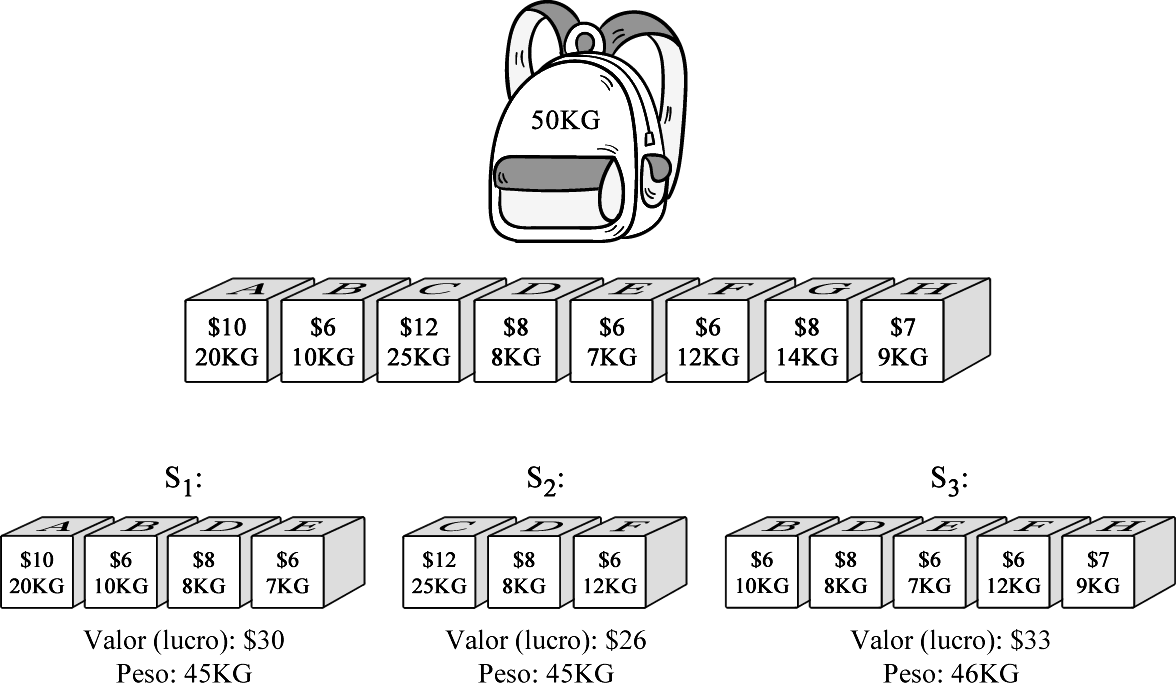
\includegraphics[width=1\textwidth]{cap_problemas/figs/mochila.png}
	\caption{\label{fig_knapsack}Exemplo para o problema da mochila mono-objetivo.}
\end{figure}

Na \autoref{fig_knapsack}, a capacidade máxima da mochila é 50Kg e existem oito itens disponíveis para se escolher. Três soluções possíveis são mostradas ($S_1$, $S_2$ e $S_3$), dentre elas, a melhor é $S_3$, pois possui o maior valor de lucro e ao mesmo tempo é válida, ou seja, respeita a restrição de capacidade (peso menor que 50Kg). No exemplo, todas as soluções estão saturadas, em outras palavras, a adição de qualquer outro item as torna inválidas.

Existem diversas estratégias para resolver o \ac{PM}. Dentre elas, as mais usadas são os algoritmos gulosos \cite{KnapsackGreedy}, a programação dinâmica \cite{KnapsackDynamic} e os algoritmos genéticos \cite{KnapsackGA}. Os algoritmos gulosos e a programação dinâmica são os mais rápidos e eficientes para resolver o PM mono-objetivo. Em contra-partida, a complexidade adicionada ao considerar mais de um objetivo inviabiliza a utilização desse tipo de algoritmo, tornando os algoritmos genéticos e demais métodos bio-inspirados as melhores opções.

O problema da mochila multiobjetivo (PMM) é similar ao mono-objetivo (PM). Sua única diferença está no fato de que cada item, ao invés de possuir um único valor (lucro), é composto de múltiplos valores. No PMM, a função $lucro(o_i)$ retorna um vetor ao invés de um único valor escalar. Cada componente (elemento) do vetor representa o valor do item $o_i$ considerando um dos objetivos. Por exemplo, considerando um PMM de 3 objetivos, cada $o_i \in O$ possui um vetor formado por três valores de lucros (um para cada objetivo). O objetivo do problema passa a ser maximizar todos os lucros ao invés de um único valor. A definição do problema da mochila utilizada neste trabalho, também utilizada em \cite{MKP}, considera apenas um peso por item e uma única restrição, referente à capacidade da mochila. Outra definição mais comum do PMM envolve a consideração de múltiplos pesos por item e múltiplas restrições para a mochila, o número de pesos e de restrições é o mesmo que o número de objetivos. Essa definição alternativa é bastante comum na literatura e foi utilizada nos trabalhos de \cite{Alaya2004,Chu1998,Ishibuchi2015}. 

O PMM já foi utilizado várias vezes para avaliar algoritmos multiobjetivos, podendo-se destacar os trabalhos de \cite{Zitzler1999}, \cite{Zitzler2002} e \cite{Zhang2007}. As instâncias do PMM utilizadas no decorrer deste trabalho foram geradas de forma aleatória e compreendem problemas da mochila com 30, 40, 50, 100 e 200 itens. Para gerar as instâncias, sortearam-se valores no intervalo (0, 1000) para os lucros e para os pesos. A capacidade da mochila foi sempre definida como 60\% da soma dos pesos.

Uma das partes mais importantes de um algoritmo de busca bio-inspirado é a modelagem da solução. Para resolver o PMM através de algoritmos genéticos, é necessário definir a representação da solução, a geração aleatória de indivíduos, o cruzamento e a mutação. A representação de uma solução no AG para o problema da mochila mono-objetivo é simples, pois a solução é representada por um vetor binário e a literatura está repleta de exemplos que podem ser resolvidos dessa maneira \cite{KnapsackGA,Hristakeva2013}. A versão \textit{many-objective} do problema não requer modificação no modelo, fazendo com que os mesmos processos de cruzamento e mutação possam ser utilizados. Nas seções a seguir, detalhe-se a representação da solução e os operadores genéticos para o PMM usados neste trabalho. A construção das soluções nos algoritmos ACO é mais elaborada e será definida no próximo capítulo.

\subsection{Representação da solução e geração da população inicial}
\label{section_representacao_pmm}
Uma solução para o PMM é representada por um vetor binário. Se a instância do problema da mochila apresenta 10 itens ao total, por exemplo, um vetor com 10 bits representa a solução. As posições do vetor representam a ausência ou a presença de cada item. Se a posição $i$ do vetor é 0, então o $i$-ésimo item não faz parte da solução. Caso contrário, se o vetor na posição $i$ vale 1, então o  $i$-ésimo item está presente na mochila. Por exemplo, em uma solução representada pelo vetor [1,0,0,1,0,1,1,0,0,0], apenas os itens 0, 3, 5 e 6 são colocados na mochila, os outros itens (1, 2, 4, 7, 8 e 9) são descartados.

Nesse cenário, a geração aleatória de uma solução consiste em sortear os valores 0 ou 1 para cada posição do vetor. Tanto a geração aleatória de um indivíduo na formação da população inicial, quanto a combinação de vetores (cruzamento) não garantem a formação de uma solução válida, ou seja, é possível que se crie um vetor, cuja soma dos pesos dos itens ultrapasse a capacidade da mochila. Portanto, após a geração de qualquer solução, seja aleatória na população inicial ou proveniente de um \textit{crossover}, é necessário executar um processo de validação da solução. Para validar um vetor binário, basta verificar a soma dos pesos associados aos itens representados por 1. Caso esse valor seja maior que a capacidade da mochila, remove-se um item aleatório. Esse processo é repetido sucessivamente, até que a solução se torne válida, ou seja, até que a soma dos pesos dos itens respeite a capacidade da mochila \cite{Ishibuchi2015}.

\subsection{Cruzamento e mutação}
O cruzamento entre duas soluções binárias, como explicado na Seção \ref{section_ag}, pode ser efetuado de diversas maneiras. Neste trabalho, foi utilizado \textit{crossover} uniforme, ou seja, o filho herda de forma aleatória os bits do pai 1 ou do pai 2. Esse processo é ilustrado na \autoref{fig_cross_uniforme}.

\begin{figure}[!htbp]
	\centering
	\renewcommand{\arraystretch}{2} 
	\begin{tabular}{rl}
		Pai 1: & 
		\renewcommand{\arraystretch}{1.15} 
		\begin{tabular}{|c|c|c|c|c|c|}
			\hline 
			\rowcolor[HTML]{F5D1CF}
			0 & 0 & 1 & 0 & 1 & 1 \\
			\hline 
		\end{tabular}
		\\
		Pai 2: & 
		\renewcommand{\arraystretch}{1.15} 
		\begin{tabular}{|c|c|c|c|c|c|}
			\hline 
			\rowcolor[HTML]{CCCCFF}
			1 & 0 & 0 & 1 & 1 & 0 \\
			\hline 
		\end{tabular}
		\\
		Máscara: & 
		\renewcommand{\arraystretch}{1.15} 
		\begin{tabular}{|c|c|c|c|c|c|}
			\hline 
			0 & 1 & 0 & 0 & 1 & 0 \\
			\hline 
		\end{tabular}
		\\
		Filho 1: & 
		\renewcommand{\arraystretch}{1.15} 
		\begin{tabular}{|c|c|c|c|c|c|}
			\hline 
			\cellcolor[HTML]{F5D1CF}0 & \cellcolor[HTML]{CCCCFF}0 & \cellcolor[HTML]{F5D1CF}1 & \cellcolor[HTML]{F5D1CF}0 & \cellcolor[HTML]{CCCCFF}1 & \cellcolor[HTML]{F5D1CF}1 \\
			\hline 
		\end{tabular}
		\\
		Filho 2: & 
		\renewcommand{\arraystretch}{1.15} 
		\begin{tabular}{|c|c|c|c|c|c|}
			\hline 
			\cellcolor[HTML]{CCCCFF}1 & \cellcolor[HTML]{F5D1CF}0 & \cellcolor[HTML]{CCCCFF}0 & \cellcolor[HTML]{CCCCFF}1 & \cellcolor[HTML]{F5D1CF}1 & \cellcolor[HTML]{CCCCFF}0 \\
			\hline 
		\end{tabular}
	\end{tabular}
	\caption{\label{fig_cross_uniforme}Exemplo de crossover uniforme}
\end{figure}

Como pode ser visto na figura \ref{fig_cross_uniforme}, o \textit{crossover} uniforme pode ser implementado com uma máscara, que é um vetor aleatório de bits que controla os genes herdados de cada filho. Se o bit na posição $i$ da máscara vale 0, então o gene do filho na posição $i$ herda o valor do pai 1, caso contrário, herda o valor do pai 2. Dessa forma, ainda é possível gerar 2 filhos: um deles usando a regra na qual o bit 0 da máscara representa o pai 1 e o bit 1 representa o pai 2 (filho 1 na figura); e o outro usando a máscara com os valores complementares (filho 2).

Após o \textit{crossover}, existe uma chance, determinada pela taxa de mutação definida para o AG, do indivíduo sofrer alguma mutação genética. Neste trabalho, foi utilizado o método mais simples de mutação para vetores binários, ou seja, a inversão de bit. Esse processo consiste em sortear uma posição aleatória do vetor e se o valor for 0, troca-se para 1, caso contrário, troca-se para 0.

\section{Problema do roteamento multicast}
\label{section_problemas_prm}

\subsection{Definição do problema}

O problema do roteamento multicast (PRM) aparece na engenharia de tráfego em redes de computadores e consiste em escolher a forma ``mais eficiente'' de transmitir uma mensagem multicast \cite{Lafeta2016}. Uma transmissão de rede pode ser do tipo unicast, multicast ou broadcast. Em transmissões unicast, conecta-se um ponto da rede a outro ponto qualquer (transmissão ponto-a-ponto). Para fazer isso de forma eficiente, é possível usar algum algoritmo capaz de encontrar o melhor caminho entre os dois pontos (e.g. \cite{Dijkstra1959}), se apenas uma métrica for utilizada. As comunicações broadcast caracterizam-se pelo fato de um nó da rede (servidor) enviar o conteúdo a todos os demais. Para obter as melhores rotas para trafegar os dados, é possível utilizar algum algoritmo capaz de determinar a árvore geradora de custo mínimo (e.g. \cite{Prim1957}), se apenas uma métrica for empregada na otimização. Em uma comunicação multicast, o objetivo é transmitir o conteúdo de um nó da rede, chamado nó de origem ou transmissor, para alguns outros nós, denominados receptores. Essa tarefa apresenta maior complexidade, mesmo no caso de uma única métrica, pois é necessário obter uma árvore de Steiner de custo mínimo, o que é mais difícil que calcular uma única rota ou construir a árvore geradora de custo mínimo \cite{Bueno2010}.

O PRM é um problema prático muito importante. Seu estudo visa o desenvolvimento de algoritmos eficientes e eficazes, proporcionando avanços na geração de rotas em redes de computadores. O objetivo desses algoritmos é encontrar soluções (rotas multicast) que permitam uma comunicação mais rápida, menos custosa e mais confiável entre dispositivos, o que é essencial em uma era onde a maioria das pessoas consomem informação e entretenimento pela Internet.

Dado que se deseja transmitir um conteúdo via uma rede de computadores, o problema, em sua versão com um único objetivo de custo, consiste em encontrar a melhor rota possível entre a fonte de dados e os vários destinos. Dado um grafo $G=(V,E)$, que representa a rede de comunicação, um nó raiz $r \in V$ (nó transmissor) e um conjunto de nós destinos $D \subset V$ (nós receptores), o PRM consiste em determinar a subárvore $T$ de $G$ enraizada em $r$ que inclui todos os vértices em $D$ e apresenta o menor custo possível. A \autoref{fig_prm_grafo} ilustra uma instância do problema de roteamento multicast. Nesse exemplo de rede de comunicação, o nó transmissor é definido por um círculo duplo (vértice 0), os nós receptores são destacados em cinza escuro (vértices 1, 8, 12 e 13) e os nós intermediários estão em cinza claro. Os números em cada aresta determinam o custo da comunicação entre os nós que ela conecta.

\begin{figure}[!htbp]
	\centering
	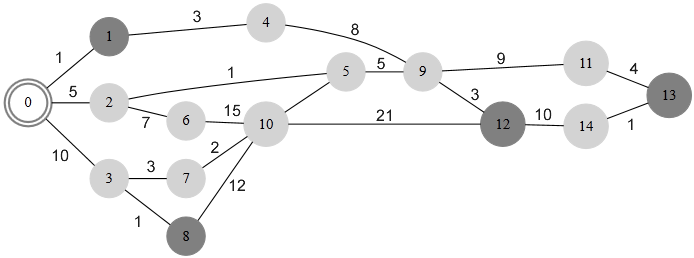
\includegraphics[width=1\textwidth]{cap_problemas/figs/prm_grafo}
	\caption{\label{fig_prm_grafo}Exemplo de uma rede de comunicação. Retirado de \cite{BuenoThesis}.}
\end{figure}

Na \autoref{fig_prm_mono}, são apresentados alguns exemplos de árvores multicast criadas a partir do grafo mostrado na figura \autoref{fig_prm_grafo}. O custo de cada árvore é dado pela soma dos custos de suas arestas. Dentre os exemplos, a árvore mais à direita possui o menor custo total: 65.

\begin{figure}[!htbp]
	\centering
	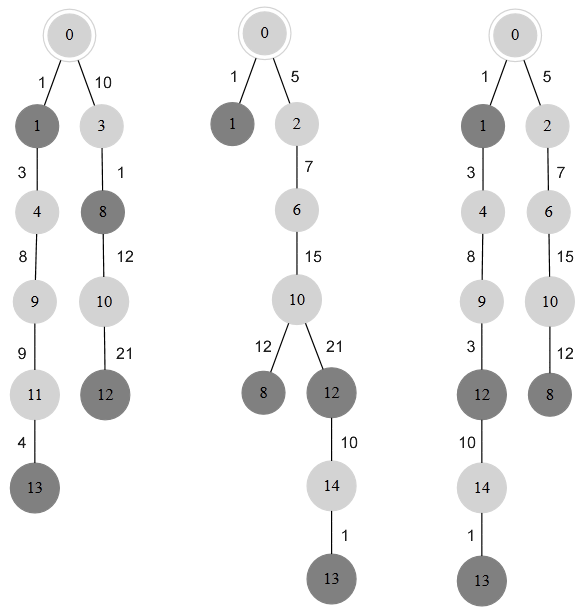
\includegraphics[width=0.8\textwidth]{cap_problemas/figs/prm_mono}
	\caption{\label{fig_prm_mono}Exemplos de árvores multicast relativos ao grafo da figura \autoref{fig_prm_grafo}. Retirado do trabalho de \cite{LafetaThesis}}
\end{figure}

O PRM original é proposto com apenas um objetivo a se otimizar e utiliza uma métrica por enlace, que é o custo. Essa métrica pode representar uma combinação de outras métricas. Entretanto, áreas que tratam da melhoria do desempenho em redes de computadores, como a engenharia de tráfego e a \ac{QoS} trouxeram uma nova necessidade para a transmissão em redes, onde a utilização de métricas distintas é mais adequada ao gerenciamento da rede. Características como distância, atraso (\textit{delay}), capacidade de tráfego e uso do tráfego são boas métricas da qualidade de serviço (QoS) em uma comunicação \cite{LafetaThesis}. Nesse contexto, este trabalho investiga uma versão multiobjetivo do problema de roteamento multicast. Nesta versão do problema, as árvores apresentadas como solução devem representar o melhor compromisso entre as métricas utilizadas.

\begin{figure}
	\centering
	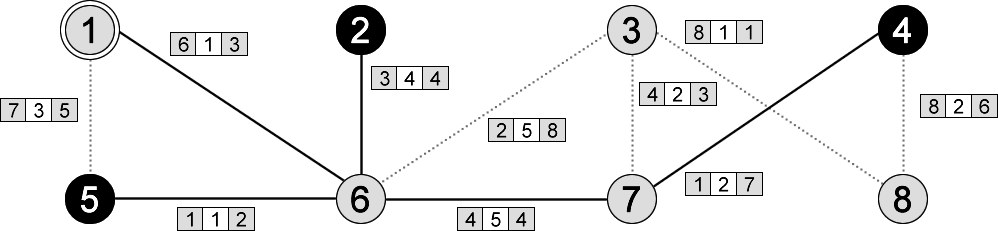
\includegraphics[width=1\textwidth]{cap_problemas/figs/prm_multi}
	\caption{\label{fig_prm_multi}Exemplo de árvore multicast no PRM multiobjetivo.}
\end{figure}

Na \autoref{fig_prm_multi} é apresentado um exemplo de rede com as métricas ``custo'' (primeiro valor), ``delay'' (segundo valor) e ``tráfego corrente'' (terceiro valor) nas arestas. As arestas representadas por linhas contínuas identificam uma árvore multicast ótima (não-dominada) para os objetivos ``custo total'', ``delay-fim-a-fim médio'' e ``utilização média dos enlaces'', descritos mais a frente no texto. Na figura, o nó 1 é a raiz e os nós com fundo escuro representam os nós destinos. Para esse exemplo, no objetivo ``utilização média dos enlaces'', considerou-se a mesma capacidade de tráfego para todos os enlaces, de forma que apenas o tráfego corrente fosse relevante.

Neste trabalho consideram-se até quatro valores de peso para um enlace da rede: custo, \textit{delay}, capacidade de tráfego e tráfego corrente, representados respectivamente pelas funções: $c()$, $d()$, $z()$ e $t()$. Por meio dessas medidas são formulados os seguintes objetivos:

\begin{enumerate} 
	\item \textbf{Custo total:} soma dos valores de custo de todas as arestas da árvore.
	\item \textbf{Delay fim-a-fim médio:} média da soma dos \textit{delays} em cada ramo da árvore. Em outras palavras, média do atraso em cada uma das comunicações cliente-servidor.
	\item \textbf{Delay fim-a-fim máximo:} maior valor para a soma de \textit{delays} dentre todos os ramos da árvore, ou seja, o maior atraso dentre todas as comunicações cliente-servidor.
	\item \textbf{\textit{Hops count}}: número de vértices na árvore.
	\item \textbf{Utilização máxima de enlaces:} considerando todas as arestas na árvore, qual delas atinge a maior utilização de banda? Matematicamente, considerando $E$ o conjunto de arestas da árvore e $\phi$ o tamanho da mensagem, essa métrica é dada por:
	\begin{equation}\max_{e \in E} \frac{t(e) + \phi}{z(e)}\end{equation}
	\item \textbf{Utilização média dos enlaces:} média da utilização de banda entre todas as arestas da árvore. Seu cálculo é similar ao da métrica anterior (utilização máxima de enlaces) e é dado por:
	\begin{equation}\frac{\sum_{e \in E} \frac{t(e) + \phi}{z(e)}}{|E|}\end{equation}
\end{enumerate}

A fim de possibilitar diversos cenários de teste para o PRM, os objetivos acima podem ser combinados de diversas maneiras, criando várias instâncias multi-objetivo do problema. Neste trabalho foram utilizadas 5 formulações (combinações) desses objetivos:

\begin{enumerate}
	\item $P_2$: formado pelos objetivos 1 e 3.
	\item $P_3$: formado pelos objetivos 1, 3 e 4.
	\item $P_4$: formado pelos objetivos 1, 3, 4 e 5.
	\item $P_5$: formado pelos objetivos 1, 3, 4, 5 e 6.
	\item $P_6$: formado pelos objetivos 1, 2, 3, 4, 5 e 6.
\end{enumerate}

O PRM foi trabalhado sobre 5 redes diferentes variando a complexidade em termos de quantidade de nós destinos, vértices e arestas. Essas redes foram retiradas do trabalho de \cite{Lafeta2016} e suas caraterísticas são apresentadas na tabela \ref{tab_prm_redes}.

\begin{table}[!htbp]
	\centering
	\caption{Definições das redes utilizadas no PRM}
	\label{tab_prm_redes}
	\begin{tabular}{r|rrr}
		Nome        & Destinos & Vértices & Arestas \\ \hline
		Rede 1 (R1) & 10       & 33       & 106     \\
		Rede 2 (R2) & 18       & 75       & 188     \\
		Rede 3 (R3) & 37       & 75       & 188     \\
		Rede 4 (R5) & 12       & 75       & 300     \\
		Rede 5 (R5) & 16       & 100      & 250     \\ \hline
	\end{tabular}
\end{table}

Para resolver o PRM através de estratégias evolutivas, é necessário, em primeiro lugar, definir a modelagem do indivíduo. Esse processo não é muito simples, pois a solução não pode ser representada por um vetor. De fato, como deve representar os caminhos entre o servidor e os múltiplos destinos em uma rede de computadores, a solução para o PRM é melhor representada por uma árvore. Dessa forma, é preciso desenvolver o processo de crossover e de mutação de acordo com essa estrutura. O operador de cruzamento deve receber duas árvores pais e gerar uma nova árvore (filha) que compartilha características de ambos os pais. O operador de mutação precisa criar uma pequena alteração na árvore que permita explorar diferentes regiões do espaço de busca, mas que não a descaracterize completamente. As seções a seguir apresentam o modelo para se aplicar um AG ao PRM.

\subsection{Representação da solução}

Como mostrado na seção \ref{section_problemas_prm}, considerando que em cada nó da rede a mensagem pode ser replicada e enviada aos próximos nós conectados, o PRM deseja encontrar a árvore que representa o processo de transmissão de menor custo que parte do nó fonte (servidor) e atinge todos os destinos. Existem duas maneiras de se representar uma solução:

\begin{enumerate}
	\item \textbf{Representação em árvore:} \cite{Bueno2010} o AG evolui a própria árvore que se deseja encontrar como solução. É um processo mais complicado que elimina a necessidade de pós-processamento. A \autoref{fig_prm_mono}, mostra alguns exemplos de árvores multicasts.
	\item \textbf{Representação em conjunto:} \cite{Baran2004} o AG evolui um conjunto de caminhos $C$, ou seja, para cada nó destino $d$, deve existir uma sequência de nós $L \in C$ que contém o caminho que leva do nó servidor (emissor) até o nó $d$. A representação em conjuntos de caminhos é mais fácil de se gerenciar, mas exige a transformação (conjunção) dos caminhos pertencentes ao conjunto em uma árvore  ao final do processo. Como diferentes árvores podem ser formadas a partir de um único conjunto de caminhos, essa representação não é tão eficiente quanto a anterior ao explorar o espaço de busca.
\end{enumerate}

Neste trabalho, optou-se por utilizar a representação em árvores.

\subsection{Geração da população inicial}

Considere um grafo da rede $G$, um nó raiz (também chamado de servidor ou emissor) $r$ e um conjunto de nós de destino $D$. Para criar uma solução aleatória no PRM, inicia-se um grafo $S$ apenas com o vértice $r$. O passo seguinte é extrair um destino aleatório $d \in D$ e, com base no grafo $G$, criar um caminho em $S$ entre qualquer um de seus vértices atuais e $d$. Após construir o caminho, $d$ com certeza será atingível a partir de qualquer vértice de $S$. O processo se repete até que todos os nós destinos estejam no grafo $S$. Por fim, o grafo $S$ é transformado em uma árvore a partir da remoção dos ciclos presentes em $S$ e da aplicação de podas dos ramos desnecessários.

Para criar o caminho aleatório entre um vértice de $S$ e um nó destino $d$, considera-se um vetor de exploração $Exp$ que, inicialmente, contém todos os nós de $S$. Enquanto o destino $d$ não é encontrado, algum nó $exp_i \in Exp$ é escolhido e todos os vértices adjacentes (conectados) a $exp_i$ são incluídos em $Exp$. Quando $d$ é encontrado, adiciona-se a $S$ o caminho necessário para sair de algum vértice de $S$ e chegar ao destino $d$.

\subsection{Cruzamento}

A estratégia de cruzamento utilizada neste trabalho para o PRM é chamada de cruzamento por caminho e foi proposta em \cite{Lafeta2016} como alternativa ao cruzamento por similaridade utilizado em trabalhos anteriores \cite{Bueno2010}. Esse tipo de cruzamento é realizado entre duas árvores $P_1$ e $P_2$ e produz um único filho $F$. O processo consiste em separar cada um dos pais em ramos e, então, para cada nó destino $d$, acrescentar a $F$ o ramo de $P_1$ ou de $P_2$ que leva a $d$. A escolha entre $P_1$ e $P_2$ é feita de forma aleatória. Assim que todos os nós destinos são atingíveis em $F$, a etapa de seleção de ramos é interrompida, os ciclos que possivelmente foram criados são removidos, e um processo de poda é realizado a fim de remover qualquer nó folha que não seja destino.

\begin{figure}[!htbp]
	\centering
	\includegraphics[width=1\textwidth]{cap_problemas/figs/prm-cruzamento-caminho}
	\caption{\label{fig_prm-cruzamento-caminho}Exemplo de cruzamento por caminho, onde o nó raiz é 0 e os destinos são \{1, 8, 11\}. Retirado de \cite{LafetaThesis}}
\end{figure}

A \autoref{fig_prm-cruzamento-caminho} representa o processo de cruzamento por caminho entre duas árvores (Pai 1 e Pai 2). No exemplo, o nó raiz é o vértice 0 e os nós destinos são o conjunto $\{1, 8, 11\}$. As setas em ``ramos do pai 1'' e ``ramos do pai 2'' representam os caminhos escolhidos em cada um dos pais para compor a árvore filha. O grafo nomeado ``reconexão'' representa o filho após a inclusão de todos os ramos. Como foi gerado um ciclo (existem dois caminhos da origem até o nó 10), o mesmo deve ser removido a fim de obter uma árvore válida. Supondo que o caminho $0 \rightarrow 12 \rightarrow 10$ tem menor custo que o caminho $0 \rightarrow 3 \rightarrow 7 \rightarrow 5 \rightarrow 10$, o nó 10 será acessado apenas a partir do nó 12. Em ``tratando factibilidade'', apresenta-se o filho após a remoção dos ciclos. Como os nós 3, 7 e 5 não são destinos, eles são removidos durante o processo de poda, resultando na última árvore (``poda'') que é o filho resultante do processo.

Para remover os ciclos, percorre-se a árvore em largura removendo qualquer aresta que adicione ciclo. No processo de poda, verificam-se todas as folhas. Se algum nó folha não for um destino, ele é removido e o processo repetido até que todos os nós folhas sejam destinos.

Após o cruzamento, realiza-se um processo de filtragem, onde todas as soluções repetidas são substituídas por novos indivíduos gerados aleatoriamente.

\section{Mutação}

A mutação em uma árvore que representa uma solução para o PRM consiste em remover parte dos nós da árvore e então reconectá-los de maneira aleatória utilizando o grafo correspondente à rede em questão. As etapas desse processo estão descritas no algoritmo \ref{alg_prm_mutacao}.

\begin{algorithm}
	\caption{Mutação para uma árvore $(A, G, qte_{arestas}, r, D)$}
	\label{alg_prm_mutacao}
	\begin{algorithmic}[1]
		\State desconectar($A$, $qte_{arestas}$)
		\State $C \gets extraiComponente(A, r)$
		\State $M \gets novoGrafo()$
		\State $M \gets mesclar(M, C)$
		\While{$|D| > 0$}
		\State $d \gets removeAleatorio(D)$
		\State $C \gets extraiComponente(A, d)$
		\If{$d \notin V(M)$}
		\State $P \gets caminhoAlearorio(C, M, G)$
		\State $M \gets mesclar(M, P)$
		\EndIf
		\State $M \gets mesclar(M, C)$
		\EndWhile
		\State $removerCiclos(M)$
		\State $podarArvore(M)$
		\State \Return $M$
	\end{algorithmic}
\end{algorithm}

O algoritmo recebe como entrada a árvore que sofrerá mutação ($A$), o grafo da rede ($G$), a quantidade de arestas a se remover na mutação ($qte_{arestas}$), o vértice raiz ($r$), e o conjunto de destinos ($D$). Na linha 1, desconecta-se a árvore através da remoção aleatória de $qte_{arestas}$ arestas. Entre as linhas 2 e 4, cria-se a estrutura para a construção da árvore ($M$). A partir da linha 5 começa o laço para reconectar todos os nós destinos à arvore. A linha 6 seleciona um destino aleatório $d$ para reconectar. Na linha 7, a componente conexa contendo $d$ é extraída de $A$ e chamada de $C$. Se não existe componente conexa com o vértice $d$, $C$ será um grafo com um único nó ($d$) e nenhuma aresta. Caso o vértice $d$ não exista na componente conexa $M$, cria-se um caminho aleatório em $M$ (com base no grafo $G$) que a conecta a $C$ (linhas 8 a 10). A construção do caminho aleatório é feita nó a nó até se encontrar uma sequência de arestas entre as duas componentes. Na linha 11, incluem-se em $M$ todas as arestas de $C$. Ao final, o mesmo pós-processamento do cruzamento por caminho é realizado: remoção de ciclos e poda da árvore (linhas 14 e 15).

Em relação à proposta utilizada em \cite{LafetaThesis}, destacam-se como diferenças a geração da população inicial e o cruzamento. Com relação à população inicial, os indivíduos gerados através do método apresentado neste trabalho apresentam diversidade um pouco maior. No que diz repeito ao cruzamento, aqui se utiliza apenas o \textit{crossover} por caminho, enquanto no trabalho anterior se utilizava também um outro tipo de cruzamento, o \textit{crossover} por similaridade.

% ----------------------------------------------------------
% Estratégias evolutivas para o PMM
% ----------------------------------------------------------
\chapter[Estratégias evolutivas para o PMM]{Estratégias evolutivas para o PMM}

Uma das partes mais importantes de um algoritmo de busca bio-inspirado é a modelagem da solução. Para os algoritmos genéticos é necessário definir a representação da solução, a geração aleatória de indivíduos, o cruzamento e a mutação. Para os ACOs, é possível utilizar a mesma representação de solução do AG, mas deve-se desenvolver um algoritmo que constrói a solução a partir de uma estrutura de feromônios e uma heurística.

A implementação de um AG para o problema da mochila mono-objetivo é trivial, pois a solução é representada por um vetor binário e a literatura está repleta de exemplos que podem ser resolvidos dessa maneira []. Um AG para o problema da mochila original pode ser encontrado em []. A versão many-objective do problema não requer nenhuma modificação no modelo, fazendo com que o mesmo processo de cruzamento e mutação possam ser utilizados. No entanto, a implementação de um ACO para o mesmo problema pode ser desafiador, já que as colônias de formigas esperam trabalhar com grafos e não arrays de bits. Um estudo extensivo relativo ao uso de ACOs para a resolução do problema da mochila com ACOs é apresenta em []. Nas seções a seguir detalhe-se a representação da solução, os operadores genéticos e a construção de soluções para o PMM usados neste trabalho.

\section{Representação da solução}
Em ambas as estratégias bio-inspiradas, AGs e ACOs, uma solução para o PMM é representada da mesma maneira: um vetor binário. Se a instância do problema da mochila apresenta 10 itens ao total, por exemplo, um vetor com 10 bits representa a solução. As posições do vetor onde o valor é 0 dizem que aquele item não será incluído na mochila, enquanto as posições que valem 1, dizem que o item será incluído na mochila. E.g. se a solução é representada pelo vetor [1,0,0,1,0,1,1,0,0,0], apenas os itens 0, 3, 5 e 6 serão colocados na mochila, os outros ficarão de fora.

\section{Cruzamento e mutação (AGs)}
O cruzamento entre duas soluções binárias, como explicado em [ref. secao ags], pode ser efetuado de diversas maneiras. Neste trabalho, foi utilizado crossover uniforme, ou seja, o filho herda de forma aleatória os bits do pai 1 ou do pai 2. Veja o exemplo da figura \ref{fig_cross_uniforme}.

\begin{figure}[!htbp]
	\label{fig_cross_uniforme}
	\caption{Exemplo de crossover uniforme}
	\centering
	\renewcommand{\arraystretch}{2} 
	\begin{tabular}{rl}
		Pai 1: & 
		\renewcommand{\arraystretch}{1.15} 
		\begin{tabular}{|c|c|c|c|c|c|}
			\hline 
			\rowcolor[HTML]{F5D1CF}
			0 & 0 & 1 & 0 & 1 & 1 \\
			\hline 
		\end{tabular}
		\\
		Pai 2: & 
		\renewcommand{\arraystretch}{1.15} 
		\begin{tabular}{|c|c|c|c|c|c|}
			\hline 
			\rowcolor[HTML]{CCCCFF}
			1 & 0 & 0 & 1 & 1 & 0 \\
			\hline 
		\end{tabular}
		\\
		Máscara: & 
		\renewcommand{\arraystretch}{1.15} 
		\begin{tabular}{|c|c|c|c|c|c|}
			\hline 
			0 & 1 & 0 & 0 & 1 & 0 \\
			\hline 
		\end{tabular}
		\\
		Filho 1: & 
		\renewcommand{\arraystretch}{1.15} 
		\begin{tabular}{|c|c|c|c|c|c|}
			\hline 
			\cellcolor[HTML]{F5D1CF}0 & \cellcolor[HTML]{CCCCFF}0 & \cellcolor[HTML]{F5D1CF}1 & \cellcolor[HTML]{F5D1CF}0 & \cellcolor[HTML]{CCCCFF}1 & \cellcolor[HTML]{F5D1CF}1 \\
			\hline 
		\end{tabular}
		\\
		Filho 2: & 
		\renewcommand{\arraystretch}{1.15} 
		\begin{tabular}{|c|c|c|c|c|c|}
			\hline 
			\cellcolor[HTML]{CCCCFF}1 & \cellcolor[HTML]{F5D1CF}0 & \cellcolor[HTML]{CCCCFF}0 & \cellcolor[HTML]{CCCCFF}1 & \cellcolor[HTML]{F5D1CF}1 & \cellcolor[HTML]{CCCCFF}0 \\
			\hline 
		\end{tabular}
	\end{tabular}
\end{figure}

Como pode ser visto na figura \ref{fig_cross_uniforme}, o crossover uniforme pode ser implementado com uma máscara, que é um vetor aleatório de bits que controla os genes herdados de cada filho. Se o bit na posição $i$ da máscara vale 0, então o filho na posição $i$ herda o valor do pai 1, caso contrário, o pai 2 fornece o valor. Dessa forma, ainda é possível gerar 2 filhos, um com a regra de que o bit 0 da máscara representa o pai 1 e o bit 1 representa o pai 2 (filho 1 na imagem), e outro com a regra inversa (filho 2).

Após o crossover, existe uma chance definida pelo AG de se mutar a solução. A mutação utilizada para o PMM foi o processo mais simples possível para vetores binários, a inversão de bit: sorteia-se uma posição aleatória do vetor, se o valor for 0, troca-se para um, caso contrário, troca-se para 0.

\section{Construção da solução (ACOs)}
As colônias de formigas foram propostas inicialmente para problemas em grafos, portanto, soa contra-intuitivo utilizá-las para o problema do mochila. Mas, como mostrado em [mkp-aco-ke], não é necessário ter um grafo para se utilizar a técnica, é possível manipular os feromônios de diversas outras formas. Para o PMM, a literatura traz três principais formas de lidar com o feromônio:

\begin{enumerate} 
	\item Depositar feromônios em cada um dos itens. Sempre que se escolher um objeto para compor a solução, incrementa-se a quantidade de feromônios nele presente. Dessa forma, a quantidade de feromônio em cada item representa a preferência para se escolhê-lo em relação aos demais. [Leguizamon and Michalewicz 1999].
	\item Criar um grafo direcionado que representa a preferência de se incluir um item $b$ logo após ter incluído um item $a$. Dessa forma, sempre que se escolher um item $a$ e posteriormente um $b$, deposita-se feromônio na aresta $(a,b)$ do grafo. Ao construir uma solução, analisa-se o último item incluído e todas as arestas no grafo que partem dele, o destino com a maior quantidade de feromônios representa o item preferível. [Fidanova 2002].
	\item A terceira estratégia proposta por [Alaya et al. 2004] utiliza um conceito semelhante a ideia anterior, mas ao invés de depositar feromônios apenas em pares consecutivos, os deposita para todos os pares de objetos existentes na solução. Por exemplo, se na solução os itens $a$, $d$ e $f$ já foram incluídos na mochila e no passo corrente adiciona-se o item $c$, o depósito de feromônios é feito nas arestas $(a,c)$, $(d,c)$ e $(f,c)$, de forma que o grafo represente a preferência de se escolher um item dado que algum outro item já tenha sido adicionado. Assim, ao construir a solução, deve-se analisar todas as arestas com origem em algum objeto já presente na solução, o destino da aresta com maior quantidade de feromônios representa o item mais desejável.
\end{enumerate}

Neste trabalho utilizou-se a estratégia 1, os feromônios são depositados nos items. Além dos feromônios, outra importante fonte de informação para se construir uma solução no ACO é a heurística, que estima o quão vantajoso é escolher um item em relação a outro. Tomando como inspiração o estudo de [mkp-aco-ke], propôs-se como heurísticas o seguinte modelo de funções:

\begin{itemize}
	\item Para cada objetivo $k$ (lucro do item), cria-se uma função de heurística $h_k$ que recebe dois parâmetros, a capacidade restante ($cr$) e o item que se deseja incluir. A capacidade restante é a diferença entre a capacidade da mochila e a soma dos pesos dos itens que já foram incluídos. A heurística é então dada por: $h_k(item, cr) = lucro_k(item) * (1 - peso(item) / cr)$.
	\item Uma heurística extra é usada exclusivamente para se referir ao peso do item: $h_{peso}(item) = 1 - peso(item) / peso\_maximo$.
\end{itemize}

Logo, o número de heurísticas no PMM é sempre o número de objetivos + 1. Tendo definido a estrutura de feromônios e as heurísticas, cabe ao algoritmo baseado em colônia de formigas construir a solução.

% ----------------------------------------------------------
% Estratégias evolutivas para o PRM
% ----------------------------------------------------------
\chapter[Estratégias evolutivas para o PRM]{Estratégias evolutivas para o PRM}

A modelagem de um algoritmo genético para o problema do roteamento multicast não é trivial, pois a solução não pode ser representada por um vetor. De fato, como deve representar os caminho entre o servidor e os múltiplos destinos em uma rede de computadores, a solução para o PRM é uma árvore. Dessa forma, é preciso desenvolver o processo de crossover e de mutação de acordo com a estrutura. O cruzamento deve receber duas árvores e gerar uma nova que compartilha características de ambos os pais, enquanto a mutação precisa criar uma pequena alteração na árvore que permita melhor explorar o espaço de busca, mas que não a descaracterize completamente.

Em contrapartida, o PRM se aproxima da definição original do ACO, pois trabalha com grafos. A diferença está no fato de que a solução é representada por uma árvore ao invés de um simples caminho, fazendo com que o depósito de feromônio e a escolha de arestas sejam desenvolvidas conforme a nova estrutura.

\section{Representação da solução}

Como mostrado na seção [seção do prm], considerando que em cada nó da rede a mensagem pode ser replicada e enviada aos próximos nós conectados, o PRM deseja encontrar a árvore que representa o processo de transmissão de menor custo que parte do nó fonte (servidor) e atinge todos os destinos. Existem duas maneiras de se representar a solução:

\begin{enumerate}
	\item Representação em árvore: o AG evolui a própria árvore que se deseja encontrar como solução. É um processo mais complicado que a alternativa a seguir, mas nenhum pós-processamento é necessário.
	\item Representação em conjunto: o AG evolui um conjunto de caminhos $C$, ou seja, para cada nó destino $d$ no problema deve existir uma lista de nós $L \in C$ que contém a sequência de nós, onde o primeiro elemento é o servidor e o último é $d$. A representação em conjuntos é mais fácil de se gerenciar, mas exige a transformação em árvore ao final do processo. Como diferentes árvores podem ser formadas a partir de um conjunto de caminhos, essa representação não é tão eficiente quanto a anterior ao explorar o espaço de busca.
\end{enumerate}

Neste trabalho optou-se por utilizar a representação 1, árvores.

\section{Inicialização dos indivíduos}

\section{Cruzamento (AG)}

O modelo de cruzamento para o PRM utilizado neste trabalho é chamado de cruzamento por caminho e foi proposto em [dissertacao do Fialho] como uma alternativa ao cruzamento por similaridade utilizado em trabalhos anteriores [Bueno e Oliveira, 2010].

O cruzamento por caminho é realizado entre duas árvores $P_1$ e $P_2$ e produz um único filho $F$. O processo consiste em separar cada um dos pais em ramos e então, para cada nó destino $d$ do PRM, acrescentar a $F$ ou o ramo de $P_1$ que leva a $d$, ou o ramo de $P_2$. A escolha entre $P_1$ e $P_2$ é feita de forma aleatória. Assim que todos os nós destinos são atingíveis em $F$, para-se a seleção de ramos, remove-se os ciclos que possivelmente foram incluídos e poda-se a árvore, excluindo qualquer nó folha que não seja um destino.

\begin{figure}[!htbp]
	\label{fig_prm-cruzamento-caminho}
	\caption{Exemplo de cruzamento por caminho}
	\centering
	\includegraphics[width=1\textwidth]{cap_estrategias-prm/figs/prm-cruzamento-caminho}
\end{figure}

A figura \ref{fig_prm-cruzamento-caminho}, retirada do trabalho de [dissertacao Fialho], representa o processo de cruzamento por caminho entre duas árvores (Pai 1 e Pai 2). No exemplo, o nó raiz (servidor) é o vértice 0 e os destinos são o conjunto $\{1, 8, 11\}$. As setas em ``ramos do pai 1'' e ``ramos do pai 2'' representam os caminhos escolhidos em cada um dos pais para compor a árvore filha. O grafo nomeado ``reconexão'' representa o filho após a inclusão de todos os ramos, e como foi gerado um ciclo, deve-se removê-lo afim de obter-se uma árvore válida. Em ``tratando factibilidade'' apresenta-se o filho após a remoção dos ciclos, como o nó folha ``5'' não é um destino, deve-se podá-lo, resultando na última árvore, ``poda'', que é o filho retornado pelo processo.

Durante o processo de cruzamento por caminho, para remover os ciclos, percorre-se a árvore em largura removendo qualquer aresta que adicione ciclo. No processo de poda, verifica-se todas as folhas, se alguma não for um destino, remove-se o nó, repetindo o processo até que todos os nós folhas sejam destinos.

\section{Mutação (AG)}

A mutação em uma árvore que representa uma solução para o PRM consiste em remover parte dos nós da árvore e então reconectá-los de maneira aleatória utilizando o grafo correspondente à rede em questão. Veja o algoritmo \ref{alg_prm_mutacao}.

\begin{algorithm}
	\caption{Mutação para uma árvore $(A, G, qte_{arestas}, r, D)$}
	\label{alg_prm_mutacao}
	\begin{algorithmic}[1]
		\State Selecione aleatoriamente $qte_{arestas}$ e remova-as de $A$
		\State Retire de $A$ a componente conexa que contém a raiz e chame-a de $C$
		\State Crie um grafo vazio $M$ para guardar o resultado da mutação
		\State Adicione todas as arestas de $C$ a $M$
		\While{$|D| > 0$}
			\State Selecione aleatoriamente um destino $d \in D$ e remova-o da lista $D$
			\State Remova de $A$ a componente conexa correspondente ao destino $d$ e coloque-a em $C$
			\If{$M$ não possui o vértice $d$}
				\State Tendo $G$ como referência, crie um caminho aleatório $P$ entre $M$ e a componente conexa $C$
				\State Adicione todas as arestas de $P$ a $M$
			\EndIf
			\State Adicione todas as arestas de $C$ a $M$
		\EndWhile
		\State Remova os ciclos em $M$, caso existam
		\State Pode a árvore $M$, removendo todos os nós folhas que não são destinos
		\State \Return $M$
	\end{algorithmic}
\end{algorithm}

No algoritmo \ref{alg_prm_mutacao} recebe-se como parâmetros a árvore a se mutar ($A$), o grafo da rede ($G$), a quantidade de arestas a se remover na mutação ($qte_{arestas}$), o vértice raiz ($r$), e o conjunto de destinos ($D$). Na linha 7, se não existe componente conexa com o vértice $d$, $C$ será um grafo com um único nó ($d$) e nenhuma aresta. Na linha 9, o caminho aleatório é construído nó a nó até se encontrar uma sequência de arestas entre as duas componentes. Ao final, o mesmo pós-processamento do cruzamento por caminho é realizado: remove-se os ciclos e poda-se a árvore.

\section{Construção da solução (ACO)}

O processo de construção da solução por um ACO no PRM deve gerar a árvore multicast com base no grafo da rede, da estrutura de feromônios e da heurística. Existem diversas maneiras de se criar tal árvore. A fim de estudar o comportamento das diferentes estratégias possíveis, aprimorá-las e determinar o melhor modelo para se utilizar no PRM, analisou-se o comportamento de cada ideia no caso mais básico possível: o PRM mono-objetivo. As ideias consideradas neste trabalho são listadas a seguir:

\begin{enumerate}
	\item A primeira estratégia, apresentada em [Baran PRM], pode ser vista como uma formiga que caminha pelo grafo até encontrar todos os destinos. A análise é feita passo a passo, considerando apenas a vizinhança do vértice corrente como possibilidades para compor a solução. O processo inicia com uma lista de exploração ($E$) que contém um único elemento: a raiz. Sorteia-se um vértice $i \in E$ e atribui-se probabilidades a todas as arestas $(i, j)$, onde $j$ é qualquer vértice não-visitado na vizinhança de $i$. $i$ é removido de $E$ caso não possua vizinhos factíveis. Um vértice $v$ é escolhido de acordo com as probabilidades calculadas, a aresta $(i, v)$ é adicionada à solução e $v$ é inserido na lista de exploração $E$. O processo é repetido até que todos os destinos tenham sido alcançados. Como etapa final, poda-se a árvore, eliminando as folhas que não representam destinos.
	\item A solução pode ser vista como os caminhos entre a raiz e cada um dos destinos, portanto, outra estratégia é imaginar que $|D|$ formigas partirão da raiz e cada uma deve encontrar um vértice $d \in D$ diferente, onde $D$ é o conjunto de nós destinos. Com cada um dos caminhos em mãos, monta-se a árvore com o cuidado de não se incluir ciclos. O último passo é a poda, que exclui qualquer vértice folha que não seja um destino. %mants
	\item Uma terceira estratégia, proposta neste trabalho, representa uma formiga fictícia que pode estar em vários locais do grafo ao mesmo tempo. Dessa forma, é possível analisar as probabilidades de todas as arestas factíveis ao mesmo tempo, ao invés de sempre escolher a composição da solução de acordo com uma vizinhança local. Ao considerar todas as possibilidades ao mesmo tempo, obtém-se um processo melhor de decisão que não tende o resultado para algum dos ramos da árvore, já que a todo momento, qualquer vértice factível pode ser incluído no resultado. O processo é iniciado a partir de uma lista de exploração ($E$) que contém todas as arestas com uma extremidade na raiz. A cada passo, calcula-se as probabilidades para toda aresta de $E$ e, de acordo com os valores obtidos, escolhe-se $e \in E$ para compor a solução. $e$ é então removido de $E$, adicionado à solução e tem todas as arestas com que compartilha um vértice adicionadas à lista de exploração (desde que ainda não tenham sido incluídas). O processo é repetido até que todos os destinos sejam atingidos. Uma poda é realizada ao final do algoritmo.
	\item Uma última estratégia é fazer um processo inverso para se construir a solução, ao invés de partir da raiz e chegar nos destinos, este modelo propõe que se utilize $|D|$ formigas, onde cada uma tem como posição inicial um destino $d \in D$ diferente. $D$ é o conjunto de vértices destinos. A ideia é que as formigas escolham seus caminhos localmente com base nas probabilidades das arestas em suas vizinhanças. Sempre que uma formiga encontrar o caminho que já foi explorado por outra formiga, ela para de explorar e meio e segue os mesmos passos realizados pelo outro agente. O processo termina quando o nó raiz foi encontrado por alguma formiga e todas as formigas tiverem se encontrado. Em linguagem matemática, o processo inicia com uma componente conexa para cada $d \in D$. Em todo passo do algoritmo, cada componente conexa é explorada a partir do último nó adicionado. Em cada componente, calcula-se as probabilidades das arestas na vizinhança do nó sendo explorado e escolhe-se, de acordo com os valores obtidos, uma novo vértice $v$ para ser adicionado à componente. Se não há arestas factíveis na vizinhança, deve-se rebobinar a exploração para um vértice anterior. Caso o nó incluído $v$ pertença a uma outra componente conexa, une-se as duas estruturas. O processo termina quando existe apenas uma componente conexa e o vértice raiz foi encontrado. Uma poda é realizada como pós-processamento da árvore. 
\end{enumerate}

Cada uma das estratégias mencionadas foi implementada e testada a fim de determinar aquela que produz as soluções de melhor qualidade. O PRM com apenas um objetivo foi o problema escolhido para avaliá-las. A fim de obter um valor como parâmetro de qualidade, também foi implementada uma versão modificada do algoritmo de Prim que aproxima a árvore multicast de menor custo. Como esperado, o algoritmo de Prim é uma opção melhor que o ACO quando se trata do PRM mono-objetivo, mas a intenção deste estudo não foi produzir um algoritmo melhor para o problema, mas sim testar as estratégias de construção de solução com o fim de utilizá-las em versões mais complexas (multi-objetivas) do PRM.

Os resultados do testes, que podem ser encontrados no apêndice [], mostraram que a estratégia número 3 representa a melhor relação entre qualidade do resultado e tempo de execução. Portanto, para todos os experimentos no PRM da seção [], esse foi o método de construção da solução utilizado.

Na lista acima, a estratégia número 3, escolhida como a melhor forma de se construir uma solução para o PRM no ACO, é explicada de maneira geral e omite alguns detalhes que são expressos no algoritmo \ref{alg_aco_prm_construir_solucao}. A ideia principal se mantem a mesma, mas se implementada da maneira como foi escrita, se torna um processo muito lento. É possível agilizar o algoritmo, sem afetar muito a qualidade das soluções, através de algumas técnicas de amostragem.

\begin{algorithm}
	\caption{Geração de solução no ACO $(G, r, D, \tau, h, E'_{size})$}
	\label{alg_aco_prm_construir_solucao}
	\begin{algorithmic}[1]
		\State Inicie uma árvore vazia $T$
		\State Inicie $E$ com todas as arestas que possuem alguma extremidade em $r$
		\State Marque $r$ como visitado
		\While{$T$ não incluir todos os vértices em $D$}
			\State Crie uma amostra aleatória $E'$ a partir da lista $E$ com $E'_{size}$ elementos
			\State Calcule as probabilidades de todas as arestas em $E'$ de acordo com $\tau$ e $h$
			\State Escolha uma aresta $e=(i,j) \in E'$ de acordo com as probabilidades
			\State Inclua $e$ em $T$
			\State Marque $j$ como visitado
			\State Calcule a vizinhança $V$ do vértice $j$
			\For{$v \in V$}
				\If{já existe aresta $a$ em $E$ que leva a $v$}
					\State Remova $a$ de $E$
					\State Calcule as probabilidades de $a$ e de $(j, v)$ de acordo com $\tau$ e $h$
					\State Sorteie uma das duas arestas de acordo com as probabilidades e adicione a vencedora em $E$
				\ElsIf{$v$ não tiver sido visitado}
					\State Inclua $(j, v)$ em $E$
				\EndIf
			\EndFor
		\EndWhile
		\State Pode a árvore $T$
		\State \Return $T$
	\end{algorithmic}
\end{algorithm}

O Algoritmo \ref{alg_aco_prm_construir_solucao} recebe como parâmetros de entrada:

\begin{itemize}
	\item $G$: o grafo que representa a rede;
	\item $r$: o nó raiz, servidor de onde parte a mensagem;
	\item $D$: conjunto de nós destinos;
	\item $\tau$: estrutura de feromônios;
	\item $h$: função heurística;
	\item $E'_{size}$: tamanho da amostra.
\end{itemize}

Trabalhar com todas as arestas possíveis é demasiadamente caro e inviável para um algoritmo em que se deseja boa performance em termos de tempo de execução. Por isso, trabalha-se com uma amostra da lista de exploração (linha 5 do algoritmo). Também a fim de se evitar o crescimento de $E$, nas linhas 12 a 16, caso um novo vértice descoberto já seja atingível a partir de alguma aresta em $E$, mantém-se em $E$ apenas uma das arestas. Para escolher qual das arestas manter, calcula-se as probabilidades de acordo com os feromônios ($\tau$) e a heurística ($h$).

% ----------------------------------------------------------
% Proposta de pesquisa
% ----------------------------------------------------------
\chapter[Algoritmo proposto]{Algoritmo proposto}
\label{chapter_macod}

O algoritmo proposto neste trabalho é baseado em colônia de formigas (ACO) e foi chamado de \textit{Many-objective Ant Colony Optimization based on Non-Dominated Sets} (MACO/NDS), em português, otimização em colônia de formigas para muitos objetivos baseada em decomposição de feromônios \cite{Franca2018}. A proposição envolve os seguintes módulos:

\begin{itemize}
	\item Modelo PMM: construção da solução para o problema da mochila multiobjetivo, apresentado na seção \ref{section_algoritmo_pmm}.
	\item Modelo PRM: construção da solução para o problema do roteamento multicast, apresentado na seção \ref{section_algoritmo_prm}.
	\item \textit{Framework} ACO: algoritmo geral desenvolvido para se trabalhar com qualquer problema discreto, apresentado na seção \ref{section_algoritmo_framework}.
\end{itemize}

Este capítulo apresenta a construção da solução no ACO para ambos os problemas (PMM e PRM). Os modelos de construção, apesar de terem sido propostos para o MACO/NDS, podem ser utilizados em qualquer algoritmo ACO. O \textit{framework} MACO/NDS, componente principal do algoritmo, é descrito em seguida na seção \ref{section_algoritmo_framework}. Nela são discutidos alguns conceitos gerais sobre a implementação multiobjetivo do ACO, bem como uma descrição mais detalhada das etapas de construção das soluções e atualização dos feromônios.

\section{Construção da solução para o PMM}
\label{section_algoritmo_pmm}

Como mostrado na seção \ref{section_representacao_pmm}, os AGs utilizam vetores binários para representar as soluções do PMM. Nos ACOs, é possível utilizar a mesma representação, entretanto, deve-se desenvolver um algoritmo que constrói a solução a partir de uma estrutura de feromônios e uma heurística. O processo de gerar as soluções é simples nos AGs, pois basta efetuar as operações de \textit{crossover} e mutação sobre os vetores binários. No entanto, a implementação de um ACO para o PMM pode ser desafiadora, já que as colônias de formigas esperam trabalhar com grafos e não vetores de bits. Um estudo extensivo relativo aos trabalhos encontrados na literatura que adotam ACOs para a resolução do problema da mochila foi realizado em \cite{Ke2010,kong2008,changdar2013,Alaya2004,Alaya2007}.

As colônias de formigas foram propostas inicialmente para problemas em grafos, e, portanto, não é intuitivo sua adaptação para outros tipos de problemas, como o problema do mochila. Entretanto, como mostrado em \cite{Ke2010}, não é necessário ter um grafo para se utilizar a técnica, sendo possível manipular os feromônios de diversas outras formas. Foram encontradas na literatura três diferentes formas de lidar com os feromônios para o problema da mochila multiobjetivo (PMM). A primeira abordagem consiste em depositar feromônios em cada um dos itens \cite{Leguizamon1999}. Sempre que um item é escolhido para compor a solução, incrementa-se a quantidade de feromônios presente no item. Dessa forma, a quantidade de feromônio em cada item representa sua preferência em relação aos demais. A segunda abordagem propõe a criação de um grafo direcionado que representa a preferência em incluir um item $b$ após a inclusão do item $a$ \cite{Fidanova2003}. Dessa forma, sempre que se escolher um item $a$ e posteriormente um $b$, deposita-se feromônio na aresta $(a,b)$ do grafo. Ao construir uma solução, analisa-se o último item selecionado e todas as arestas no grafo que partem dele. O destino com a maior quantidade de feromônios representa o item preferível. A terceira estratégia foi proposta por \cite{Alaya2004} utiliza um conceito semelhante a abordagem anterior. Entretanto, ao invés de depositar feromônios apenas em pares consecutivos, eles são depositados para todos os pares de objetos existentes na solução. Por exemplo, se na solução os itens $a$, $d$ e $f$ estão na mochila e no passo atual adiciona-se o item $c$, o depósito de feromônios é feito nas arestas $(a,c)$, $(d,c)$ e $(f,c)$, de forma que o grafo represente a preferência de se escolher um item dado que algum outro item já tenha sido selecionado. Assim, ao construir a solução, deve-se analisar todas as arestas com origem em algum item já presente na solução, o destino da aresta com maior quantidade de feromônios representa o item mais desejável. Neste trabalho utilizou-se a primeira estratégia que deposita os feromônios diretamente nos itens.

Além dos feromônios, outra importante fonte de informação para se construir uma solução no ACO é a heurística. Ela é responsável por estimar o quão vantajoso é escolher um item em relação a outro. Tomando como inspiração o estudo de \cite{Ke2010}, nossas implementações do ACO utilizam como heurísticas o seguinte modelo de funções:

\begin{itemize}
	\item Para cada objetivo $k$ (lucro do item), cria-se uma função de heurística $h_k$ que recebe dois parâmetros, a capacidade restante ($cr$) e o item que se deseja incluir. A capacidade restante é a diferença entre a capacidade da mochila e a soma dos pesos dos itens que já foram incluídos. A heurística é então dada por: \[h_k(item, cr) = lucro_k(item) \times (1 - \frac{peso(item)}{cr})\]
	\item Uma heurística extra é usada exclusivamente para se referir ao peso do item, a qual é dada por: \[h_{peso}(item) = 1 - \frac{peso(item)}{peso\_maximo}\]
\end{itemize}

Logo, o número de heurísticas no PMM é sempre o número de objetivos + 1. Tendo definido a estrutura de feromônios e as heurísticas, para construir uma solução, o algoritmo recebe a função heurística ($h$) e um vetor de feromônios ($\tau$). Inicialmente, a lista de exploração $Exp$ contém todos os itens possíveis, a probabilidade $p$ de cada item $exp_i \in Exp$ é calculada de acordo com a heurística de $exp_i$ ($h(exp_i)$) e a quantidade de feromônios no item $tau_i$, como na fórmula seguinte:

\[p(exp_i) = \frac{\tau_i^\alpha + h(exp_i)^\beta}{\sum_{j \gets 0}^{tamanho(Exp)} \tau_j^\alpha + h(exp_j)^\beta}\]

O próximo item na solução é escolhido de acordo com as probabilidades calculadas em uma espécie de roleta, onde, quanto maior o valor de probabilidade ($p(exp_i)$), maior a chance do item ser escolhido. Após ter selecionado um item, recalcula-se a lista $Exp$ para que contenha apenas itens válidos para a solução, isto é, remove-se qualquer elemento de $Exp$ que, se incluído na solução, excede a capacidade da mochila. O processo é repetido até que $Exp$ seja uma lista vazia.

A fim de reduzir a complexidade do algoritmo de construção da solução para o PMM, ao invés de se utilizar a lista completa de itens possíveis ($Exp$), utiliza-se uma amostra desse conjunto ($Exp'$). $Exp$ é calculado normalmente, mas ao submeter-se o conjunto para o cálculo de probabilidades e roleta, no lugar de $Exp$, é utilizado $Exp'$, uma amostra aleatória de tamanho fixo $Exp'_{size}$ (parâmetro do algoritmo) da lista completa $Exp$.

\section{Construção da solução para o PRM}
\label{section_algoritmo_prm}

A modelagem de um algoritmo genético para o problema do roteamento multicast não é trivial, pois deve-se representar os caminhos entre o servidor e os múltiplos destinos em uma rede de computadores, ou seja, uma árvore. Em contrapartida, o PRM se aproxima da definição original do ACO, pois trabalha com grafos. Dessa forma, a modelagem de um ACO para o PRM é mais natural que a modelagem de um AG.

O processo de construção da solução por um ACO no PRM deve gerar a árvore \textit{multicast} com base no grafo da rede, da estrutura de feromônios e da heurística. Existem diversas maneiras de se criar tal árvore. A fim de estudar o comportamento das diferentes estratégias possíveis, aprimorá-las e determinar o melhor modelo para se utilizar no PRM, analisou-se o comportamento de cada ideia no caso mais básico possível: o PRM mono-objetivo. As ideias consideradas neste trabalho são listadas a seguir:

\begin{enumerate}
	\item A primeira estratégia, apresentada em \cite{Pinto2005}, pode ser vista como uma formiga que caminha pelo grafo até encontrar todos os destinos. A análise é feita passo a passo, considerando apenas a vizinhança do vértice corrente como possibilidades para compor a solução. O processo inicia com uma lista de exploração ($Exp$) que contém um único elemento: a raiz. Sorteia-se um vértice $i \in Exp$ e atribui-se probabilidades a todas as arestas $(i, j)$, onde $j$ é qualquer vértice não-visitado na adjacência de $i$. $i$ é removido de $Exp$ caso não possua vizinhos factíveis. Um vértice $v$ é escolhido de acordo com as probabilidades calculadas (conforme à seção \ref{section_otimizacao_aco_construcao}), a aresta $(i, v)$ é adicionada à solução e $v$ é inserido na lista de exploração $Exp$. O processo é repetido até que todos os destinos tenham sido alcançados. Como etapa final, poda-se a árvore, eliminando as folhas que não representam destinos.
	\item Uma solução pode ser vista como os caminhos entre a raiz e cada um dos destinos. Portanto, outra estratégia é imaginar que $|D|$ formigas partirão da raiz e cada uma deve encontrar um vértice $d \in D$ diferente, sendo $D$ o conjunto de nós destinos. Com os caminhos para todos os nós destinos definidos, monta-se a árvore evitando a ocorrência de ciclos. Por fim, realiza-se a poda da árvore para excluir qualquer vértice folha que não seja um destino. %mants
	\item Uma terceira estratégia é proposta neste trabalho. Ela adota uma representação de formiga fictícia que pode estar em vários locais do grafo ao mesmo tempo (formiga com sobreposição quântica). Dessa forma, é possível analisar as probabilidades de todas as arestas factíveis ao mesmo tempo, ao invés de sempre escolher a composição da solução de acordo com uma vizinhança local. Ao considerar todas as possibilidades ao mesmo tempo, obtém-se um processo melhor de decisão que não apresenta qualquer tendência (viés) para algum dos ramos da árvore, já que a todo momento, qualquer vértice factível pode ser incluído no resultado. O processo é iniciado a partir de uma lista de exploração ($Exp$) que contém todas as arestas conectadas ao nó raiz. A cada passo, calcula-se as probabilidades para toda aresta de $Exp$ e, de acordo com os valores obtidos, escolhe-se $exp_i \in Exp$ para compor a solução. $exp_i$ é então removida de $Exp$, adicionada à solução e tem todas suas arestas adicionadas à lista de exploração, desde que ainda não tenham sido incluídas. O processo é repetido até que todos os destinos sejam atingidos. Uma poda é realizada ao final do processo.
	\item A última estratégia consiste em construir a solução de forma inversa. Ao invés de partir da raiz e chegar aos destinos, este modelo propõe que se utilize $|D|$ formigas, onde cada uma tem como posição inicial um nó destino $d \in D$ diferente. A ideia é que as formigas escolham seus caminhos localmente com base nas probabilidades das arestas em suas vizinhanças. Sempre que uma formiga encontrar o caminho que já foi explorado por outra formiga, ela para de explorar e segue os mesmos passos realizados pelo outro agente. O processo termina quando o nó raiz foi encontrado por alguma formiga e todas as formigas tiverem se encontrado em algum vértice. Em outras palavras, o processo inicia com uma componente conexa para cada $d \in D$. Em todo passo do algoritmo, cada componente conexa é explorada a partir do último nó adicionado. Nesse processo, calcula-se as probabilidades das arestas na vizinhança do nó explorado e escolhe-se, de acordo com os valores obtidos, um novo vértice $v$ para ser adicionado à componente. Se não há arestas factíveis na vizinhança, deve-se retroceder para um vértice anterior. Caso o nó incluído $v$ pertença a uma outra componente conexa, elas se unem. O processo termina quando existe apenas uma componente conexa e o vértice raiz foi encontrado. Por fim, uma poda é realizada como pós-processamento da árvore. 
\end{enumerate}

Cada uma das estratégias mencionadas foi implementada e testada a fim de determinar aquela que produz as soluções de melhor qualidade para o PRM. Para obter um valor como parâmetro de qualidade, também foi implementada uma versão modificada do algoritmo de Prim \cite{Prim1957} que aproxima a árvore \textit{multicast} de menor custo. Como esperado, o algoritmo de Prim é uma opção melhor que o ACO quando se trata do PRM mono-objetivo. Entretanto, a intenção deste estudo não é produzir um algoritmo melhor para o problema, mas avaliar as estratégias de construção de solução com o objetivo de escolher aquela que será empregada em versões mais complexas (multiobjetivo) do PRM.

Os resultados dos testes, que podem ser encontrados no capítulo de experimentos (seção \ref{section_experimentos_etapa2}), mostram que nossa estratégia (formiga com sobreposição quântica) representa a melhor relação entre qualidade do resultado e tempo de execução. Portanto, para todos os demais experimentos no PRM, foi o método de construção da solução utilizado.

Durante a implementação da estratégia, foram adotadas algumas técnicas de amostragem a fim de agilizar o algoritmo, sem afetar significativamente a qualidade das soluções. A descrição detalhada dessa implementação é apresentada no Algoritmo \ref{alg_aco_prm_construir_solucao}, que recebe como parâmetros de entrada:

\begin{itemize}
	\item $G$: o grafo que representa a rede;
	\item $r$: o nó raiz, servidor de onde parte a mensagem;
	\item $D$: conjunto de nós destinos;
	\item $\tau$: estrutura de feromônios;
	\item $h$: função heurística;
	\item $Exp'_{size}$: tamanho da amostra.
\end{itemize}

\begin{algorithm}
	\caption{Geração de solução no ACO $(G, r, D, \tau, h, Exp'_{size})$}
	\label{alg_aco_prm_construir_solucao}
	\begin{algorithmic}[1]
		\State Inicie uma árvore vazia $T$
		\State Inicie $Exp$ com todas as arestas que possuem alguma extremidade em $r$
		\State Marque $r$ como visitado
		\While{$T$ não incluir todos os vértices em $D$}
		\State Crie uma amostra aleatória $Exp'$ a partir da lista $Exp$ com $Exp'_{size}$ elementos
		\State Calcule as probabilidades de todas as arestas em $Exp'$ de acordo com $\tau$ e $h$
		\State Escolha uma aresta $e=(i,j) \in Exp'$ de acordo com as probabilidades
		\State Inclua $e$ em $T$
		\State Marque $j$ como visitado
		\State Calcule a vizinhança $V$ do vértice $j$
		\For{$v \in V$}
		\If{já existe aresta $a$ em $Exp$ que leva a $v$}
		\State Remova $a$ de $Exp$
		\State Calcule as probabilidades de $a$ e de $(j, v)$ de acordo com $\tau$ e $h$
		\State Sorteie uma das duas arestas de acordo com as probabilidades e adicione a vencedora em $Exp$
		\ElsIf{$v$ não tiver sido visitado}
		\State Inclua $(j, v)$ em $Exp$
		\EndIf
		\EndFor
		\EndWhile
		\State Pode a árvore $T$
		\State \Return $T$
	\end{algorithmic}
\end{algorithm}

Trabalhar com todas as arestas possíveis é demasiadamente caro e inviável para um algoritmo em que se deseja bom desempenho em termos de tempo de execução. Por isso, trabalha-se com uma amostra da lista de exploração (linha 5 do algoritmo). Outro processo de simplificação também é empregado para evitar o crescimento exagerado de $Exp$ durante a etapa de exploração, nas linhas 12 a 16. Nesse processo, caso um novo vértice descoberto já seja atingível a partir de alguma aresta em $Exp$, mantém-se em $Exp$ apenas uma das arestas. Para escolher qual das arestas manter, calcula-se as probabilidades de acordo com os feromônios ($\tau$) e a heurística ($h$).

Com relação às heurísticas no PRM, uma função é construída para cada métrica de rede presente na formulação de objetivos. Por exemplo, no problema $P_4$, cujos objetivos envolvem as métricas custo, \textit{delay}, tráfego e capacidade, quatro heurísticas são criadas:

\[ \begin{cases} 
h_1(e) = 1 - custo(e) \\
h_2(e) = 1 - delay(e) \\
h_3(e) = 1 - trafego(e) \\
h_4(e) = capacidade(e)
\end{cases}
\]

Onde $custo(e)$, $delay(e)$, $trafego(e)$ e $capacidade(e)$ correspondem, respectivamente, ao valor normalizado entre 0 e 1 para o custo, \textit{delay}, tráfego e capacidade da aresta $e$. Na heurística $h_4$ não é feito o complemento da função, pois essa é a única métrica que deve ser maximizada.

\section{\textit{Framework} MACO/NDS}
\label{section_algoritmo_framework}

O MACO/NDS se baseia na ideia do AEMMD de se criar tabelas de dominância para diferentes combinações possíveis de objetivos, adaptando-na para um modelo de colônia de formigas.

A multiplicidade de objetivos impõe que algumas mudanças sejam feitas na ideia original do ACO. Isso envolve responder as seguintes perguntas:

\begin{itemize}
	\item Como representar os diferentes objetivos no depósito de feromônio?
	\item Como compor as múltiplas heurísticas em uma única função?
\end{itemize}

De acordo com \cite{Alaya2007}, essas questões podem ser resolvidas através de uma das seguintes opções:

\begin{itemize}
	\item \textbf{Várias colônias e múltiplos feromônios $(m+1, m)$:} considerando $m$ o número de objetivos, esse modelo utiliza $m + 1$ colônias de formigas e $m$ estruturas de feromônios. Cada colônia é associada a um único objetivo e otimiza apenas esse objetivo através de sua própria estrutura de feromônios. Uma colônia adicional, que representa o conjunto de todos os objetivos, utiliza os feromônios das outras colônias de forma aleatória. Ao criar uma solução, sorteia-se alguma das estruturas de feromônios para se utilizar a cada passo. Outra proposta, no modelo $(m+1, m)$ é utilizar a soma de todas as estruturas de feromônios ao criar uma solução na colônia extra. Quanto as heurísticas, cada colônia utiliza a função referente a seu objetivo, enquanto a colônia extra utiliza o somatório de todas as funções de heurística.
	\item \textbf{Colônia e feromônio únicos $(1,1)$:} este modelo utiliza apenas uma colônia de formigas e uma estrutura de feromônios. Assim como no modelo anterior, as heurísticas são somadas para montar uma solução. A única estrutura de feromônios representa todos os objetivos. A atualização dos feromônios se dá através de um arquivo que mantém todas as soluções não-dominadas encontradas. Toda solução não-dominada contribui com a mesma quantidade de feromônios, já que, de fato, são indiferenciáveis em termos de qualidade.
	\item \textbf{Única colônia e vários feromônios $(1,m)$:} considerando $m$ o número de objetivos, esse modelo utiliza uma colônia de formigas e $m$ estruturas de feromônios. Assim como nos demais modelos, as heurísticas são somadas para montar uma solução. A cada passo da construção da solução, sorteia-se aleatoriamente a estrutura de feromônios a se utilizar. Cada estrutura de feromônios representa um objetivo e sua atualização é feita a cada iteração do algoritmo, de acordo com a melhor solução encontrada considerando aquele objetivo.
\end{itemize}

Em \cite{Alaya2007}, os experimentos mostraram que o terceiro modelo ($1,m$) gera os melhores resultados quando aplicado ao problema da mochila multiobjetivo. Dentre os ACOs multiobjetivos investigados, o MOACS se encaixa na segunda abordagem (1,1), adaptando apenas o modo de lidar com a heurística, enquanto o MOEA/D-ACO adota a primeira estratégia (m,m), pois trabalha com múltiplas formigas e várias estruturas de feromônios, apesar da quantidade exata de formigas e tabelas de feromônios não ser ditada pelo número de objetivos.

Nosso algoritmo (MACO/NDS), não pertence a nenhuma das categorias apresentadas por \cite{Alaya2007}, mas se aproxima da estratégia (1,m), pois lida com uma única colônia e múltiplos feromônios. A grande diferença é que o número de estruturas de feromônio não é igual a quantidade de objetivos, mas ao número de possíveis combinações entre os objetivos, de forma semelhante ao que ocorre no AEMMD \cite{Lafeta2017}. Além disso, o processo de cálculo da heurística e de atualização dos feromônios se difere substancialmente da ideia original do modelo $(1,m)$. O MACO/NDS, se baseia na ideia de decomposição, ou seja, ao invés de trabalhar diretamente com todos os objetivos, o problema é atacado em várias frentes com quantidades reduzidas de funções. Desta forma, evita-se o problema onde não é possível classificar a população devido ao alto número de soluções não-dominadas em espaços de dimensionalidade alta \cite{Deb2014}. O Algoritmo \ref{alg_macod_geral} apresenta uma visão em alto nível do MACO/NDS.

\begin{algorithm}[!htbp]
	\caption{Algoritmo geral do MACO/NDS}
	\label{alg_macod_geral}
	\begin{algorithmic}[1]
		\State $P \gets criarEstruturasDeFeromonios()$
		\State $P_{ativo} \gets \{P[0], P[1], ..., P[4]\}$
		\While{condição de parada não for atingida}
		\State $S \gets criarSolucoes(P_{ativo})$
		\State $atualizarArquivo(P[tamanho(P) - 1].arquivo, S)$
		\State $S_{nd} \gets P[tamanho(P) - 1].arquivo$
		\State $atualizarEstruturasDeFeromonios(P_{ativo}, S_{nd})$
		\EndWhile
		\State \Return $S_{nd}$
	\end{algorithmic}
\end{algorithm}

O primeiro passo do MACO/NDS (linha 1 do Algoritmo \ref{alg_macod_geral}) é criar as estruturas de feromônio $P = \{p_1, p_2, ..., p_i, ..., p_n\}$, uma para cada combinação possível de objetivos (análogo ao processo do AEMMD apresentado na seção \ref{section_aemmd}). Para um problema de seis objetivos, por exemplo, são criadas 57 estruturas ($|P| = 57$). Cada $p_i \in P$ é responsável por um subproblema e guarda as seguintes informações:

\begin{itemize}
	\item \textbf{Valores:} corresponde aos valores dos feromônios em si, os quais são inicializados com o menor valor possível.
	\item \textbf{Objetivos:} determina os objetivos do subproblema em questão. É um vetor binário de tamanho $m$ (número de objetivos), onde cada o bit 1 representa um objetivo que faz parte do problema e o bit 0 indica aqueles que não pertencem ao problema.
	\item \textbf{Arquivo:} conjunto de soluções não-dominadas que apareceram até o momento para o subproblema em questão.
	\item \textbf{Convergência:} indica a convergência do arquivo. Começa em 0 e incrementa em 1 sempre que o arquivo sofre alterações durante uma iteração (época).
	\item \textbf{$\beta$:} importância da heurística no cálculo de probabilidades ao construir uma solução. Sempre inicializado com o valor do parâmetro $\beta$ passado ao MACO/NDS.
\end{itemize}

As estruturas de feromônios são utilizadas no processo de construção da solução e devem ser atualizadas em toda iteração do algoritmo. Manipular todas as estruturas de feromônios de $P$ (57 estruturas, no caso de seis objetivos) é computacionalmente caro e inviável. Por essa razão, define-se um número máximo de estruturas para se trabalhar em um dado momento. Em ambos os problemas utilizados neste trabalho (PMM e PRM), foi utilizado um limite de cinco estruturas de feromônios ativas simultaneamente. A ordem de ativação dos elementos de $P$ é determinada pela sua ordem em $P$. Por isso, é importante a sequência em que as estruturas são criadas: os primeiros subproblemas instanciados são aqueles que representam um menor número de  objetivos, ou seja, combinações 2 a 2. Em seguida, instancia-se os subproblemas de 3 objetivos e, assim por diante, até que a última estrutura de feromônios com o número total de objetivos seja criada.

Na linha 2 do Algoritmo \ref{alg_macod_geral}, os cinco subproblemas mais simples são ativados. Na atualização dos feromônios, assim que algum dos subproblemas passa a não contribuir satisfatoriamente para o conjunto de soluções, é desativado em favor do próximo problema mais complexo ainda não utilizado. Dessa forma, o conjunto de soluções do MACO/NDS cresce gradualmente, partindo das decomposições mais simples em direção às mais complexas.

O laço principal do ACO, iniciado na linha 3 do algoritmo, consiste em gerar soluções e atualizar as estruturas de feromônios ativas. Na linha 4, é construído o conjunto de soluções $S$ de acordo com os feromônios em $P_{ativo}$, esse processo é detalhado na seção \ref{section_macod_solutions}. Nas linha 5 e 6, o arquivo de soluções não dominadas geral (considerando todos os objetivos) é atualizado e chamado de $S_{nd}$. Por último, na linha 7, as soluções de $S_{nd}$ são utilizadas para atualizar cada uma das estruturas em $P_{ativo}$. Após o término do laço principal, o algoritmo MACO/NDS retorna todas as soluções não dominadas encontradas ($S_{nd}$).

O processo de se atualizar as estruturas de feromônio a partir das soluções não dominadas encontradas (linha 7) é mostrado com mais detalhes no Algoritmo \ref{alg_macod_dist}, que recebe como entrada o conjunto $P_{ativo}$ e o conjunto de soluções $S_{nd}$

\begin{algorithm}[!htbp]
	\caption{Atualização das estruturas de feromônios}
	\label{alg_macod_dist}
	\begin{algorithmic}[1]
		\For{$i \gets 0 até tamanho(P_{ativo})$}
		\State $a \gets P_{ativo}[i]$
		\State $dif = atualizarArquivo(a, S_{nd})$
		\State $A \gets dif.added$
		\State $R \gets dif.removed$
		\If{|A| > 0}
		\State $a.\beta \gets \beta$
		\State $depositarFeromonios(a, A)$
		\State $evaporarFeromonios(a, R)$
		\Else
		\State $a.convergencia \gets a.convergencia + 1$
		\State $a.\beta \gets a.\beta \times \beta_{inc}$
		\If{$a.convergencia > MAX_{convergencia}$}
		\State $P_{ativo}[i] \gets proxima\_estrura\_feromonios$,
		\State $a.convergencia \gets 0$
		\EndIf
		\EndIf
		\EndFor
	\end{algorithmic}
\end{algorithm}

O Algoritmo \ref{alg_macod_dist} mostra a atualização das estruturas de feromônios no MACO/NDS. O processo iterativo (linha 1) passa por todas as estruturas em $P_{ativo}$. Nas linhas 2 a 5, a estrutura atual é chamada de $a$ e seu arquivo é atualizado de acordo com as soluções no conjunto $S_{nd}$. Além disso, todas as soluções adicionadas ao arquivo são guardadas na lista $A$, enquanto todas as removidas são colocadas em $R$. As linhas 7, 8 e 9 são executadas apenas se o arquivo de $a$ foi atualizado. Na linha 7, o valor $beta$ de $a$ é reinicializado para o valor original (parâmetro $\beta$ do algoritmo); na linha 8, os valores de feromônio de $a$ são incrementados de acordo com as soluções em $A$; e na linha 9, os valores de feromônios de $a$ são decrementados de acordo com as soluções em $R$. As operações das linhas 8 e 9 são detalhadas na seção \ref{section_macod_pheromones}, sobre a atualização dos feromônios. Os valores de feromônios são alterados apenas se o arquivos tiver sido modificado, por outro lado, caso o arquivo não tenha sofrido atualização, as linhas 11 a 16 são executadas. Na linha 11, a convergência de $a$ é incrementada em 1. Na linha 12, o valor $\beta$ de $a$ é modificado de acordo com a constante pré-definida $\beta_{inc}$, a intenção é que se diminua a importância das heurísticas sempre que a busca parecer estagnada. Assim que novas soluções são encontradas, o valor $\beta$ de $a$ volta ao normal (linha 7). No caso da implementação utilizada neste trabalho, para diminuir a importância da heurística, deve-se aumentar o valor de $\beta$. A quantidade em que se deve alterar esse valor dependerá do problema. Nos nossos experimentos (descritos no capítulo \ref{chapter_experimentos}), o valor de $\beta$ aumenta em 10\% tanto no PMM quanto no PRM. Por último, nas linhas 14 e 15, se a convergência de $a$ atingiu o limite máximo $MAX_{convergencia}$, substitui-se a estrutura $a$ em $P_{ativo}$ pelo próximo $p_i \in P$, reiniciando o valor da convergência de $a$ para caso seja necessário utilizá-la novamente no decorrer do algoritmo. O valor da constante $MAX_{convergencia}$ utilizado neste trabalho foi 10.

\subsection{Construção das soluções}
\label{section_macod_solutions}

As soluções em colônias de formigas são construídas a partir do grupo de feromônios ativo ($P_{ativo}$), das heurísticas ($H$) e dos valores de $\alpha$ e $\beta$. Os feromônios são criados e atualizados no decorrer do algoritmo, enquanto os demais são parâmetros de entrada. A heurística é uma função que estima a qualidade de uma parcela da solução, ex: arestas em problemas que envolvam grafos, como o PRM, e itens em problemas representados por vetores, como o PMM. Enquanto o parâmetro $\alpha$ determina a importância do feromônio ao tomar uma decisão a respeito da composição da solução, $\beta$ representa a importância da heurística.

No MACO/NDS existem múltiplas estruturas de feromônios e heurísticas. Portanto, para que se possa construir uma solução, é necessário antes escolher quais valores de feromônio e qual função de heurística serão utilizados. 

As estruturas de feromônios são recebidas pelo processo de construção das soluções através da lista de estruturas ativas do MACO/NDS ($P_{ativo}$), ou seja, 5 conjuntos de feromônios são utilizados por vez. De maneira circular, cada solução utiliza uma única estrutura de feromônios para ser construída, ou seja, a primeira solução é criada a partir da primeira estrutura de $P_{ativo}$, a segunda a partir da segunda e, assim por diante, até a sexta solução que utiliza novamente a primeira estrutura de $P_{ativo}$.

Com relação às heurísticas, o MACO/NDS utiliza o mesmo processo proposto em \cite{Riveros2016}. Admite-se um grau de importância para cada função: 0 (não importante), 1 (importante) ou 2 (muito importante). O valor de importância é sorteado para cada heurística e funciona como um peso. A função única utilizada para construir a solução é a soma ponderada das heurísticas considerando os pesos sorteados.

O processo geral para se construir as soluções é exposto no Algoritmo \ref{alg_macod_solucao}.

\begin{algorithm}
	\caption{Construção das soluções}
	\label{alg_macod_solucao}
	\begin{algorithmic}[1]
		\State $S \gets \emptyset$
		\For{$i \gets 0$ até $nro\_maximo\_solucoes$}
		\State $W \gets \emptyset$
		\For {$j \gets 0$ até $|H|-1$}
		\State $W[j] \gets random(0,2)$
		\EndFor
		\State $h(x) \gets \sum_{i \gets 0}^{|H|-1}\frac{H[i](x) * W[i]}{\sum\limits_{w \in W}w}$
		\State $p \gets P_{ativo}[i \pmod{|P_{ativo}|}]$
		\State $s \gets gerarSolucao(p.feromonios, h, \alpha, p.\beta)$
		\State $S \gets S \cup \{s\}$
		\EndFor
		\State \Return $S$
	\end{algorithmic}
\end{algorithm}

O Algoritmo \ref{alg_macod_solucao} apresenta o processo geral para se construir um conjunto de soluções. Na linha 1, $S$ é inicializado como um conjunto vazio. A partir da linha 2, um laço é executado para gerar todas as soluções necessárias. Nas linhas 3 a 6, $|H|$ valores entre 0 e 2 (inclusive) são sorteados para um vetor $W$. Na linha 7, é criada a função heurística correspondente à combinação de todas as heurísticas de acordo com as importâncias sorteadas. Na linha 8, chama-se de $p$ a estrutura de feromônio atual. A nova solução é criada na linha 9 de acordo com os feromônios de $p$, a função heurística $h$, o parâmetro do $\alpha$ do algoritmo e o valor $\beta$ de $p$. Na linha 10, a nova solução é incluída no conjunto de soluções $S$. Por fim, na linha 12, retorna-se o conjunto $S$ de soluções.

Na linha 6 do algoritmo \ref{alg_macod_solucao} constrói-se a solução em si. Esse processo depende exclusivamente do problema em questão e representa a principal parte na elaboração do modelo para um algoritmo baseado em colônia de formigas. No caso do problema da mochila multiobjetivo, a estratégia utilizada é aquela descrita em \ref{section_algoritmo_pmm}. Para o problema do roteamento multicast, a estratégia de construção da solução foi apresentada em \ref{section_algoritmo_prm}.

\subsection{Atualização dos feromônios}
\label{section_macod_pheromones}

A atualização dos feromônios no MACO/NDS pode ser de dois tipos:

\begin{enumerate}
	\item \textbf{Depósito:} a partir de uma solução, adiciona-se uma quantidade $\delta$ ao feromônio correspondente à cada partícula da solução. No caso de um problema em grafos, por exemplo, para cada aresta da solução, incrementa-se em $\delta$ o feromônio daquela aresta.
	\item \textbf{Evaporação:} similar ao depósito, mais ao invés de incrementar o feromônio em $\delta$, decrementa-se.
\end{enumerate}

O depósito de feromônio ocorre quando novas soluções não-dominadas são encontradas. A evaporação no MACO/NDS, diferentemente da maioria dos algoritmos baseados em ACO, não ocorre para todos os feromônios em todas as iterações. Ao invés disso, o feromônio só é decrementado quando uma solução deixa de ser não-dominada (ver algoritmo \ref{alg_macod_geral}).

Dada uma solução $s$ do problema do roteamento multicast (PRM), se $s$ deve ser reforçada (depósito), cada aresta $e$ da árvore $s$ incrementa o valor correspondente na estrutura de feromônios em um fator $\delta$. Matematicamente, esse processo de depósito é definido por:

\[\delta(e) = (1 - pesos(e)) \times \rho\]

Sendo, $pesos(e)$ é a média dos pesos normalizados na aresta $e$, e $\rho$ é a taxa de evaporação (parâmetro do MACO/NDS). Se $s$ deve ser desencorajada (evaporação), os valores na matriz de feromônios correspondentes às arestas de $s$ devem ser decrementados em $\delta$.

Dada uma solução $s$ do problema da mochila multiobjetivo (PMM), se $s$ deve ser reforçada (depósito), cada item $i$ de $s$ incrementa o valor correspondente na estrutura de feromônios em um fator $\delta$. O cálculo do depósito no PMM é dado por:

\[\delta(i) = lucros(i) \times (1 - peso(i) / peso\_{max}) \times \rho\]

Onde $lucros(i)$ é a média dos valores normalizados de lucro do item $i$, e $peso\_{max}$ é o maior peso dentre todos os itens. Se $s$ deve ser desencorajada (evaporação), os valores no vetor de feromônios correspondentes aos itens de $s$ devem ser decrementados em $\delta$.

%O fator de incremento de feromônio em ACOs multiobjetivos é normalmente fixo e independente tanto da solução quanto da partícula (aresta ou item). A ideia de se basear a quantidade de feromônios na qualidade da partícula é utilizada em nosso modelo devido aos experimentos realizados mais a frente no texto, na etapa 2 do capítulo \ref{chapter_experimentos} (seção \ref{section_experimentos_etapa2}).


% ----------------------------------------------------------
% Experimentos e avaliação dos resultados
% ----------------------------------------------------------

\chapter[Experimentos]{Experimentos}
\label{chapter_experimentos}

Neste capítulo são apresentados os experimentos realizados durante a pesquisa. Esses experimentos visam avaliar o desempenho de diversas abordagens bio-inspiradas (algoritmos evolutivos e baseados em colônias de formigas), incluindo o algoritmo proposto nesta dissertação (MACO/NDS), quando empregadas na resolução de dois problemas discretos com muitos objetivos. 

Para facilitar a análise dos resultados, esses experimentos foram divididos em 4 etapas distintas de acordo com os objetivos desejados. Na primeira etapa, cinco algoritmos evolutivos multiobjetivos (AEMOs), encontrados da literatura, foram avaliados em problemas discretos de 2 a 6 objetivos. O objetivo dessa etapa é analisar o comportamento desses algoritmos de acordo com o número de objetivos tratados. Na segunda etapa, a fim de se desenvolver a base para a elaboração do algoritmo MACO/NDS pra o PRM multiobjetivo, avaliaram-se diversas estratégias para a construção de uma solução em um ACO mono-objetivo. A terceira etapa de experimentos contou com o algoritmo proposto (MACO/NDS) em sua versão final, ou seja, com a melhores estratégias observadas na segunda etapa de experimentos. O objetivo da terceira etapa foi avaliar o MACO/NDS contra os algoritmos \textit{many-objective} vistos até então (NSGA-III, MOEA/D, AEMMT e AEMMD) nos dois problemas (PMM e PRM) em instâncias com formulações a partir de 4 objetivos. A última etapa de experimentos conta com a adição de mais três métodos em relação a etapa anterior: o SPEA2-SDE, o MOEA/D-ACO e o MOACS. O objetivo dessa última seção é avaliar o comportamento dos algoritmos em instâncias mais complexas dos problemas da mochila e do roteamento. Além disso, na quinta etapa, é utilizada a métrica hipervolume na avaliação dos resultados.

\section{Ambiente de teste}

Esta seção descreve a metodologia empregada nos experimentos, isto é, os algoritmos utilizados, as formas de avaliação e a apresentação dos resultados. Os seguintes algoritmos multiobjetivos foram utilizados nesses experimentos:

\acresetall
\begin{itemize}
	\item \ac{NSGA-II} \cite{Deb2002};
	\item \ac{NSGA-III} \cite{Deb2014};
	\item \ac{SPEA2} \cite{Zitzler2002};
	\item \ac{SPEA2-SDE} \cite{Spea2SDE};
	\item \ac{MOEA/D} \cite{Zhang2007};
	\item \ac{MEAMT}. Nesta dissertação, referenciamos esse trabalho pelo nome proposto originalmente em português, \ac{AEMMT} \cite{Brasil2013};
	\item \ac{MEANDS}. Nesta dissertação, referenciamos esse trabalho pelo nome proposto originalmente em português, \ac{AEMMD} \cite{Lafeta2017};
	\item \ac{MOEA/D-ACO} \cite{Ke2013};
	\item \ac{MOACS} \cite{Riveros2016}
	\item e o ACO proposto: \ac{MACO/NDS}.
\end{itemize}

Todos esses algoritmos foram avaliados considerando dois problemas discretos multiobjetivos: o \ac{PMM} e o Problema \ac{PRM}. A fim  de verificar o comportamento dos algoritmos em relação ao número de objetivos, diversas formulações foram consideradas, avaliando-se problemas desde dois até seis objetivos. Assim como o número de funções objetivo, a topologia da rede (PRM) e a quantidade de itens (PMM) também afetam a complexidade. Portanto, elaboraram-se instâncias diferentes para cada problema. No PRM, são consideradas seis redes de diferentes complexidades, as quais também foram utilizadas em \cite{LafetaThesis}. No PMM variou-se a quantidade de itens em 30, 40, 50, 100 e 200.

Parte das métricas utilizadas para avaliar os algoritmos são paramétricas, ou seja, dependem do conhecimento prévio sobre a fronteira de Pareto do problema. Como foi inviável a obtenção do Pareto exato para cada instância, antes de executar os experimentos, foi calculado um conjunto aproximado para a fronteira de Pareto de cada um dos cenários de teste. Tal conjunto aproximado, denominado ``Pareto aproximado'' ou ``fronteira de Pareto aproximada'', foi obtido através de várias execuções de todos os algoritmos utilizados nos experimentos sobre o cenário. Além disso, no caso das instâncias de redes do PRM, esses resultados foram comparados com os Paretos aproximados obtidos em \cite{Lafeta2017}.

Considerando as quatro etapas de experimentos, foram usadas 4 métricas multiobjetivo para se avaliar o desempenho dos algoritmos, além do tempo de execução. São elas:

\begin{itemize}
	\item \textbf{\ac{ER}}: sendo $S$ o conjunto de soluções encontrado pelo algoritmo e P a fronteira de Pareto aproximada. A taxa de erro é porcentagem de soluções que aparecem em ambos os conjuntos S e P, como mostra a fórmula a seguir.
	\begin{equation}
		ER = \frac{\sum\limits_{s \in S} e(s)}{|S|}, \quad
		e(s) = 
		\begin{cases} 
			0 & s \in P \\
			1 & s \notin P
		\end{cases}
	\end{equation}
	\item \textbf{\ac{GD}}: mede a distância das soluções no conjunto encontrado pelo algoritmo (S) para as soluções mais próximas na fronteira de Pareto aproximada (P). A distância euclidiana ($dist$) de cada $s \in S$ é medida em relação a cada $p \in P$, a menor distância para $p$ de cada $s$ é então elevada ao quadrado e adicionada à soma. Ao final, retorna-se o valor da raiz quadrada do somatório dividido pela quantidade de elementos em $S$. A fórmula a seguir ilustra o processo.
	\begin{equation}GDp = \frac{\sqrt{\sum\limits_{s \in S} \min\limits_{p \in P} dist(s, p)^2}}{|S|}\end{equation}
	\item \textbf{\ac{GDp}}: similar à definição anterior, mas ao invés de considerar todas as soluções no cálculo de distância, considera apenas aquelas que não fazem parte do Pareto aproximado, ou seja, elimina do cálculo as distâncias que valem 0.
	\item \textbf{\ac{PS}}: número absoluto de soluções encontradas (S) que fazem parte do Pareto aproximado (P). Como mostra a fórmula a seguir.
	\begin{equation}
		PS = \sum\limits_{s \in S} a(s), \quad
		a(s) = 
		\begin{cases} 
			1 & s \in P \\
			0 & s \notin P
		\end{cases}
	\end{equation}
	\item \textbf{\ac{HV}}: \cite{Bradstreet2012}: métrica multiobjetivo que independe do conhecimento prévio da fronteira de Pareto. Mede o volume da figura geométrica $m$-dimensional (sendo $m$ o número de objetivos) formada pelas distâncias entre as soluções encontradas e um ponto de referência $p_{ref}$. As coordenadas de $p_{ref}$ são diferentes para cada cenário (problema, formulação de objetivos e instância) e são determinadas pelo pior valor encontrado em cada um dos objetivos considerando a união das soluções dos Paretos obtidos em cada execução. Se o PMM de 5 objetivos e 100 itens é executado 10 vezes, por exemplo, extraem-se os 10 resultados e colocam-se as soluções em um único conjunto $S_{todos}$. Varre-se $S_{todos}$ procurando pelo pior valor em cada uma das 5 coordenadas e cria-se uma solução fictícia para os valores encontrados. Essa solução fictícia é então utilizada como ponto de referência ($p_{ref}$) para o PMM de 5 objetivos e 100 itens. Em nossos experimentos, foi utilizada a implementação do cálculo de hipervolume descrito em \citeonline{Bradstreet2012}.
	\item Tempo: tempo médio, em segundos, necessário para a execução do algoritmo. Foi aferido a partir das diferenças de tempo entre o momento em que o algoritmo inicia a execução até o momento quando retorna o conjunto de soluções encontradas. O valor final do tempo é obtido através da média entre três execuções.
\end{itemize}

Para obter os valores dessas métricas, nas seções \ref{section_experimentos_etapa1} e \ref{section_experimentos_etapa3}, foram feitas 100 execuções de cada algoritmo em cada cenário. Na Seção \ref{section_experimentos_etapa4}, que utiliza o hipervolume, o número de execuções foi 30. O número reduzido de execuções na última etapa se deve à maior dificuldade em se calcular o hipervolume em relação às demais métricas. Uma ressalva também é feita quanto ao tempo de execução, que foi calculado separadamente através da média aritmética de três execuções isoladas de cada algoritmo em cada cenário. O número reduzido de experimentos para se obter os valores de tempo se deve a dois fatores. Primeiramente, executar cada algoritmo isoladamente em uma máquina leva muito tempo, o que torna inviável a execução de vários testes. Além disso, o tempo não varia muito de uma execução para outra, fazendo com que a média entre três simulações seja suficiente. 

A apresentação dos resultados é feita de três formas: gráficos, tabelas e testes de hipótese. Os gráficos utilizam barras para mostrar os valores da média dos resultados de cada métrica considerando todas as execuções para o algoritmo e cenário indicados. Nos casos onde foram obtidos os desvios padrões, linhas verticais, sobre as barras nos gráficos, são utilizadas para apresentá-los. Os mesmos valores mostrados de maneira gráfica nas seções a seguir, podem ser encontrados em forma de tabelas no apêndice \ref{ape_tabelas_exp}. Além disso, em alguns dos experimentos, é utilizado o testes de hipótese teste Z (\textit{Z test}) para confirmar se a superioridade de algum algoritmo em relação aos outros possui significância estatística. O teste de hipótese é apresentado através de uma tabela, onde cada linha representa um cenário e cada coluna uma métrica de desempenho, os sinais de ``$>$'' e ``$<$'' indicam se o método em teste obteve resultado significativamente maior ou menor em relação a seu adversário, enquanto o sinal ``$=$'' indica que não é possível determinar de forma significativa. Além dos sinais, no teste de hipótese, as células são coloridas em verde, caso o algoritmo em teste tenha obtido melhor desempenho, em vermelho, caso o desempenho tenha sido pior e em branco, nos casos onde o desempenho foi similar.

\section{Etapa 1: Análise Comparativa dos Algoritmos Evolutivos}
\label{section_experimentos_etapa1}

Os experimentos apresentados nesta seção serviram como base para a elaboração de um artigo publicado no \ac{BRACIS} \cite{Franca2017}. Na elaboração do artigo, o autor da presente dissertação implementou e efetuou os testes com o PMM, enquanto os testes com o PRM foram realizados por outro autor e também estudante de pós-graduação Thiago Fialho Lafetá, que investigou o PRM em sua própria dissertação \cite{LafetaThesis}. Posteriormente, o PRM também foi implementado e o novo ambiente serviu de base para os experimentos descritos nas próximas seções. Os resultados no PRM gerados pelo aluno Thiago Fialho são apresentados nessa seção, pois suas conclusões foram importantes na definição dos próximos passos da dissertação.

Na primeira etapa, foram realizados experimentos visando a análise comparativa dos AGs multiobjetivos NSGA-II, NSGA-III, SPEA2, MOEA/D e AEMMT nos problemas da mochila e do roteamento multicast. O número de objetivos varia entre dois e seis e, no PRM, três redes são testadas, enquanto o PMM lida com instâncias de 30, 50 e 100 itens. Além dos cinco algoritmos mencionados, avalia-se também uma pequena modificação no AEMMT chamada de AEMMT-f que remove o limite no tamanho do arquivo de soluções não-dominadas (\textit{free size}). As avaliações dos algoritmos são feitas com base em métricas relacionadas ao Pareto aproximado calculado e permitem um melhor entendimento sobre o comportamento dos algoritmos. Isso facilitou a identificação de pontos fortes e fracos de cada estratégia, ajudando na elaboração do MACO/NDS, que é o novo algoritmo proposto neste trabalho.

Neste etapa, os algoritmos NSGA-II, NSGA-III, SPEA2, MOEA/D e AEMMT foram avaliados em diferentes cenários dos dois problemas investigados (PRM e PMM). Ao todo, 30 cenários de teste foram considerados (15 para cada problema):

\begin{itemize}
	\item PMM: 5 formulações de objetivos (2 a 6) e 3 instâncias (30, 50 e 100 itens). Os valores de cada objetivo e dos pesos dos itens são gerados aleatoriamente para cada instância do problema, conforme descrito na Seção \ref{section_problemas_pmm}.
	\item PRM: 5 formulações de objetivos ($P_2$ a $P_6$) e 3 redes ($R_1$, $R_2$ e $R_3$). Tanto as formulações quanto as redes estão descritas na Seção \ref{section_problemas_prm}.
\end{itemize}

Para cada um dos cenários foi obtida uma fronteira de Pareto aproximada, através de múltiplas execuções dos 5 algoritmos testados. A Tabela \ref{table_exp1_paretos} mostra a cardinalidade de cada Pareto encontrado.

\begin{table}[!htbp]
	\centering
	\caption{Fronteira de Pareto estabelecida para os cenários investigados na primeira etapa de experimentos}
	\label{table_exp1_paretos}
	\begin{tabular}{c|rrr|rrr}
		& \multicolumn{3}{c|}{\textbf{PRM}} & \multicolumn{3}{c}{\textbf{PMM}} \\ \hline
		Objetivos & R1         & R2       & R3        & 30 itens  & 50 itens & 100 itens \\ \hline
		2         & 14         & 9        & 6         & 15        & 67       & 170       \\
		3         & 30         & 18       & 17        & 106       & 501      & 6288      \\
		4         & 122        & 72       & 60        & 425       & 986      & 88374*    \\
		5         & 424        & 326      & 551       & 1765      & 5213     & 176868*   \\
		6         & 1196       & 657      & 1078      & 5800      & 35760*   & 248198*   \\ \hline
	\end{tabular}
\end{table}

Na Tabela \ref{table_exp1_paretos}, a quantidade de elementos nos paretos do PMM é demasiadamente grande para as formulações de objetivos com 100 itens. Isso acontece porque o espaço de busca do problema da mochila cresce exponencialmente com o número de itens. Esse crescimento é potencializado com o número de objetivos considerado, ou seja, quanto maior a quantidade de funções objetivos na formulação, maior o número de soluções que serão não-dominadas. O asterisco ao lado de alguns valores no PMM significa que não foi possível estabilizar o Pareto, ou seja, a cada rodada de execuções dos algoritmos, novas soluções eram encontradas. Tal comportamento motivou a realização dos experimentos da etapa 4 (Seção \ref{section_experimentos_etapa4}), nos quais não se usa um Pareto pré-definido para se avaliar os algoritmos. Apesar disso, os resultados para o problema de 100 itens ainda são relevantes, pois mesmo que os Paretos não sejam estáveis, comparam-se as execuções dos algoritmos contra o conjunto de soluções encontradas por todos eles, possibilitando determinar o algoritmo com melhor potencial para encontrar boas soluções nos diferentes cenários dos problemas multiobjetivos.

Os resultados utilizados no cálculo das métricas de desempenho $ER$, $GD$ e $PS$ foram obtidos a partir da média entre 100 execuções de cada algoritmo. Nessas execuções foram adotados os parâmetros de configuração listados na Tabela \ref{table_exp1_parametros}. Os parâmetros foram retirados de trabalhos anteriores \cite{LafetaThesis, Brasil2013, Ishibuchi2015}. Na tabela, o asterisco em ``número de gerações'' é para dizer que nem todos os algoritmos seguem esse parâmetro. O AEMMT executa 9 mil gerações para o PRM e 7500 para o PMM. Isso acontece, pois esse algoritmo gera apenas 1 filho por ciclo no PRM e apenas 2 no PMM necessitando, portanto, de mais gerações para fazer o mesmo número de avaliações de novos indivíduos. No problema da mochila com 100 itens, devido à complexidade do problema, dobrou-se a quantidade de gerações. Ainda na tabela \ref{table_exp1_parametros}, o termo ``variável'' indica que a taxa de mutação adotada varia de acordo com a instância do problema. Nos experimentos realizados, foi empregada uma taxa de mutação de 6\% para o PMM de 30 itens, 4\% para o de 50 itens e 2\% para o de 100 itens, similar aos valores utilizados em \cite{Ishibuchi2015}. Entretanto, o mesmo valor foi empregado em todos os algoritmos.

\begin{table}[!htbp]
	\caption{Parâmetros utilizados pelos AEMOs na 1ª etapa, de acordo com o problema tratado.}
	\label{table_exp1_parametros}
	\begin{center}
		\begin{tabular}{c|r|r}
			\textbf{Parâmetro} & \textbf{(A) PRM} &  \textbf{(B) PMM} \\ %\hline
			\hline
			Tamanho da população                    &    90 &      150 \\ %\hline
			Número de gerações*                     &   100 (9000*) &      100 (7500*) \\ %\hline
			Taxa de crossover                       & 100\% &    100\% \\ %\hline
			Taxa de mutação                         &  20\% & variável \\ %\hline
			Tamanho da vizinhança (MOEA/D)          &    10 &       10 \\ %\hline
			Tamanho das tabelas (AEMMT)             &    30 &       50 \\ %\hline
			Tamanho da tabela de dominância (AEMMT) &    90 &      150 \\ %\hline
			Número de subdivisões (NSGA-III)        &     8 &        8 \\
			\hline
		\end{tabular}
	\end{center}
\end{table}

As Figuras \ref{fig_exp1_pmm_30}, \ref{fig_exp1_pmm_50} e \ref{fig_exp1_pmm_100} mostram, respectivamente, os resultados para o PMM de 30, 50 e 100 itens. Nas Figuras \ref{fig_exp1_prm_r1}, \ref{fig_exp1_prm_r2} e \ref{fig_exp1_prm_r3} são apresentados os resultados dos algoritmos para o PRM considerando as redes $R_1$, $R_2$ e $R_3$, respectivamente. Uma análise consolidada, considerando a média entre as três instâncias de cada problema, é apresenta nas Figuras \ref{fig_exp1_pmm_todos} (PMM) e \ref{fig_exp1_prm_todos} (PRM).

\begin{figure*}[!htbp]
	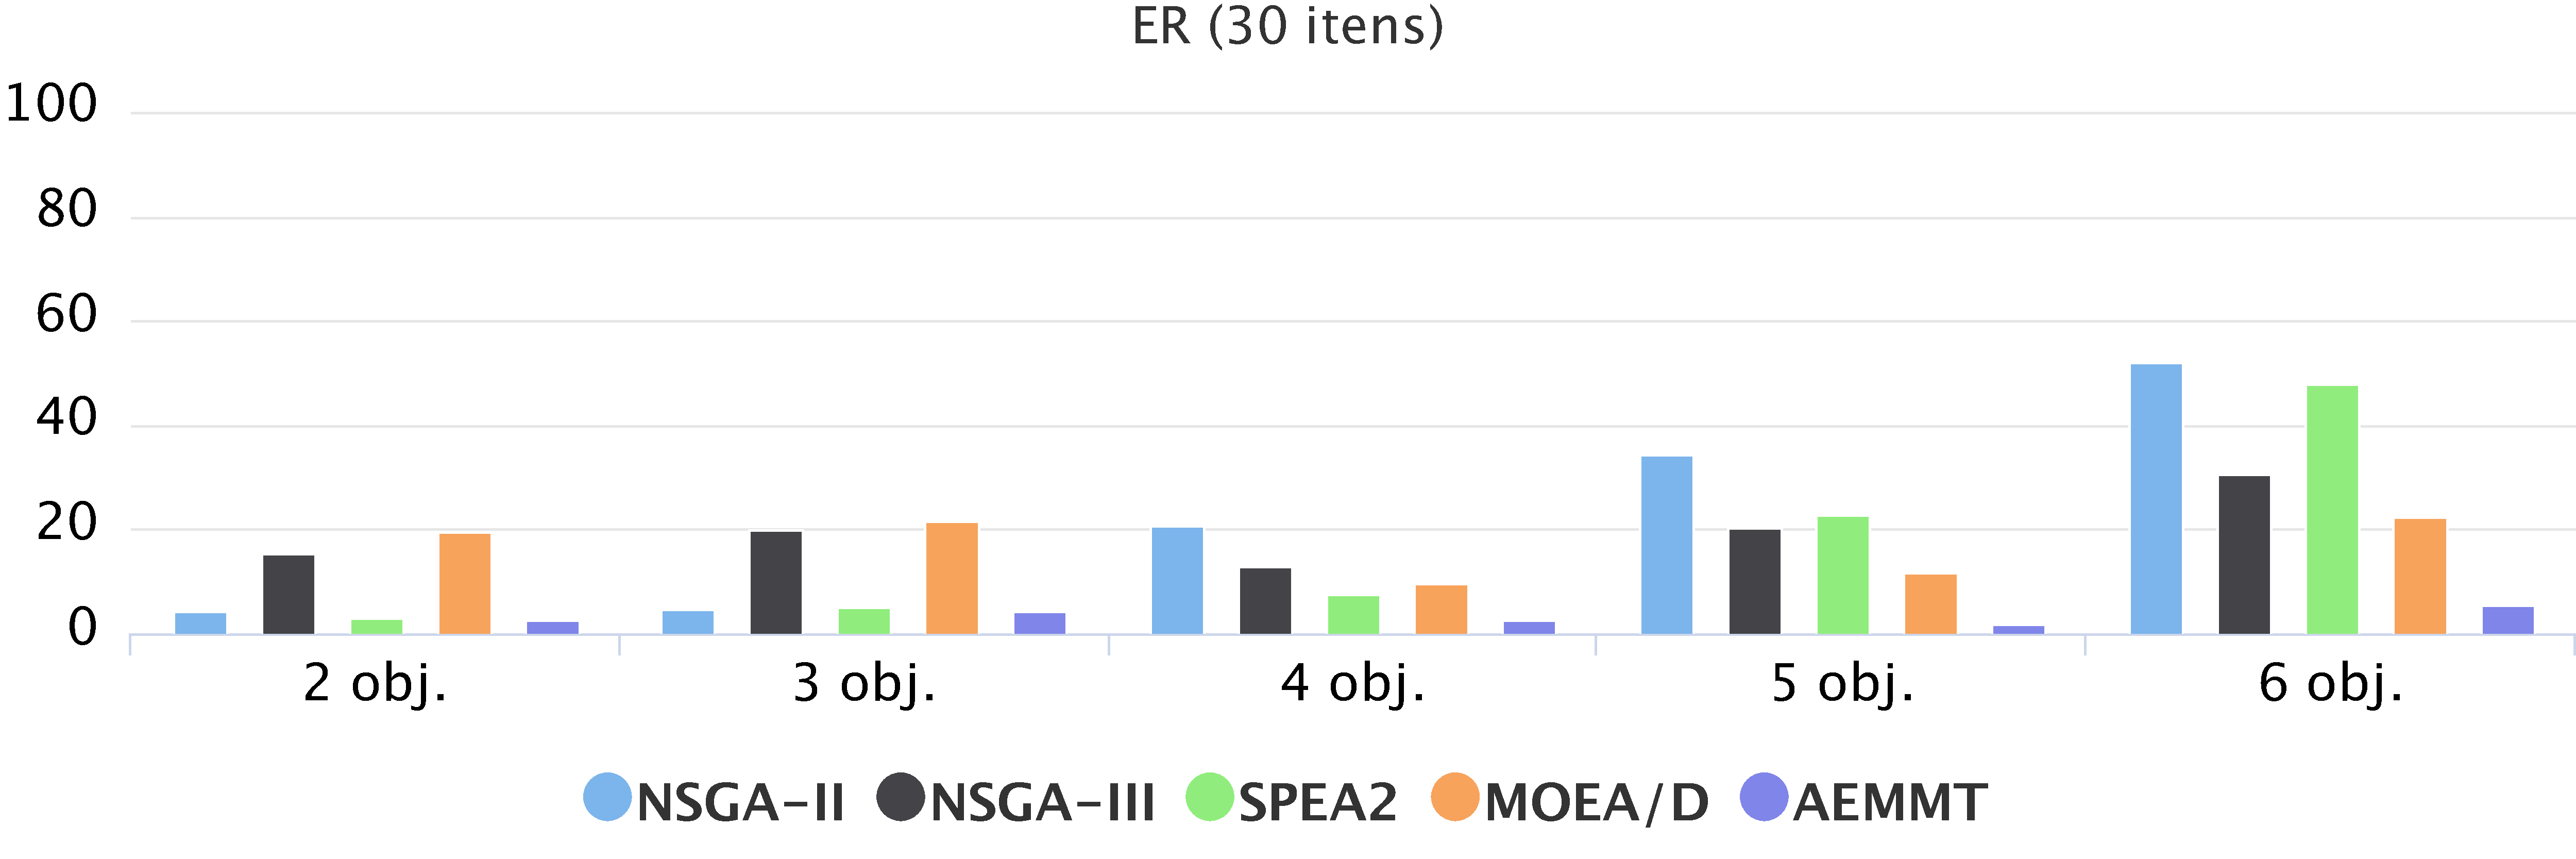
\includegraphics[width=1\textwidth]{cap_experimentos/figs/etapa1/er-mkp-30}
	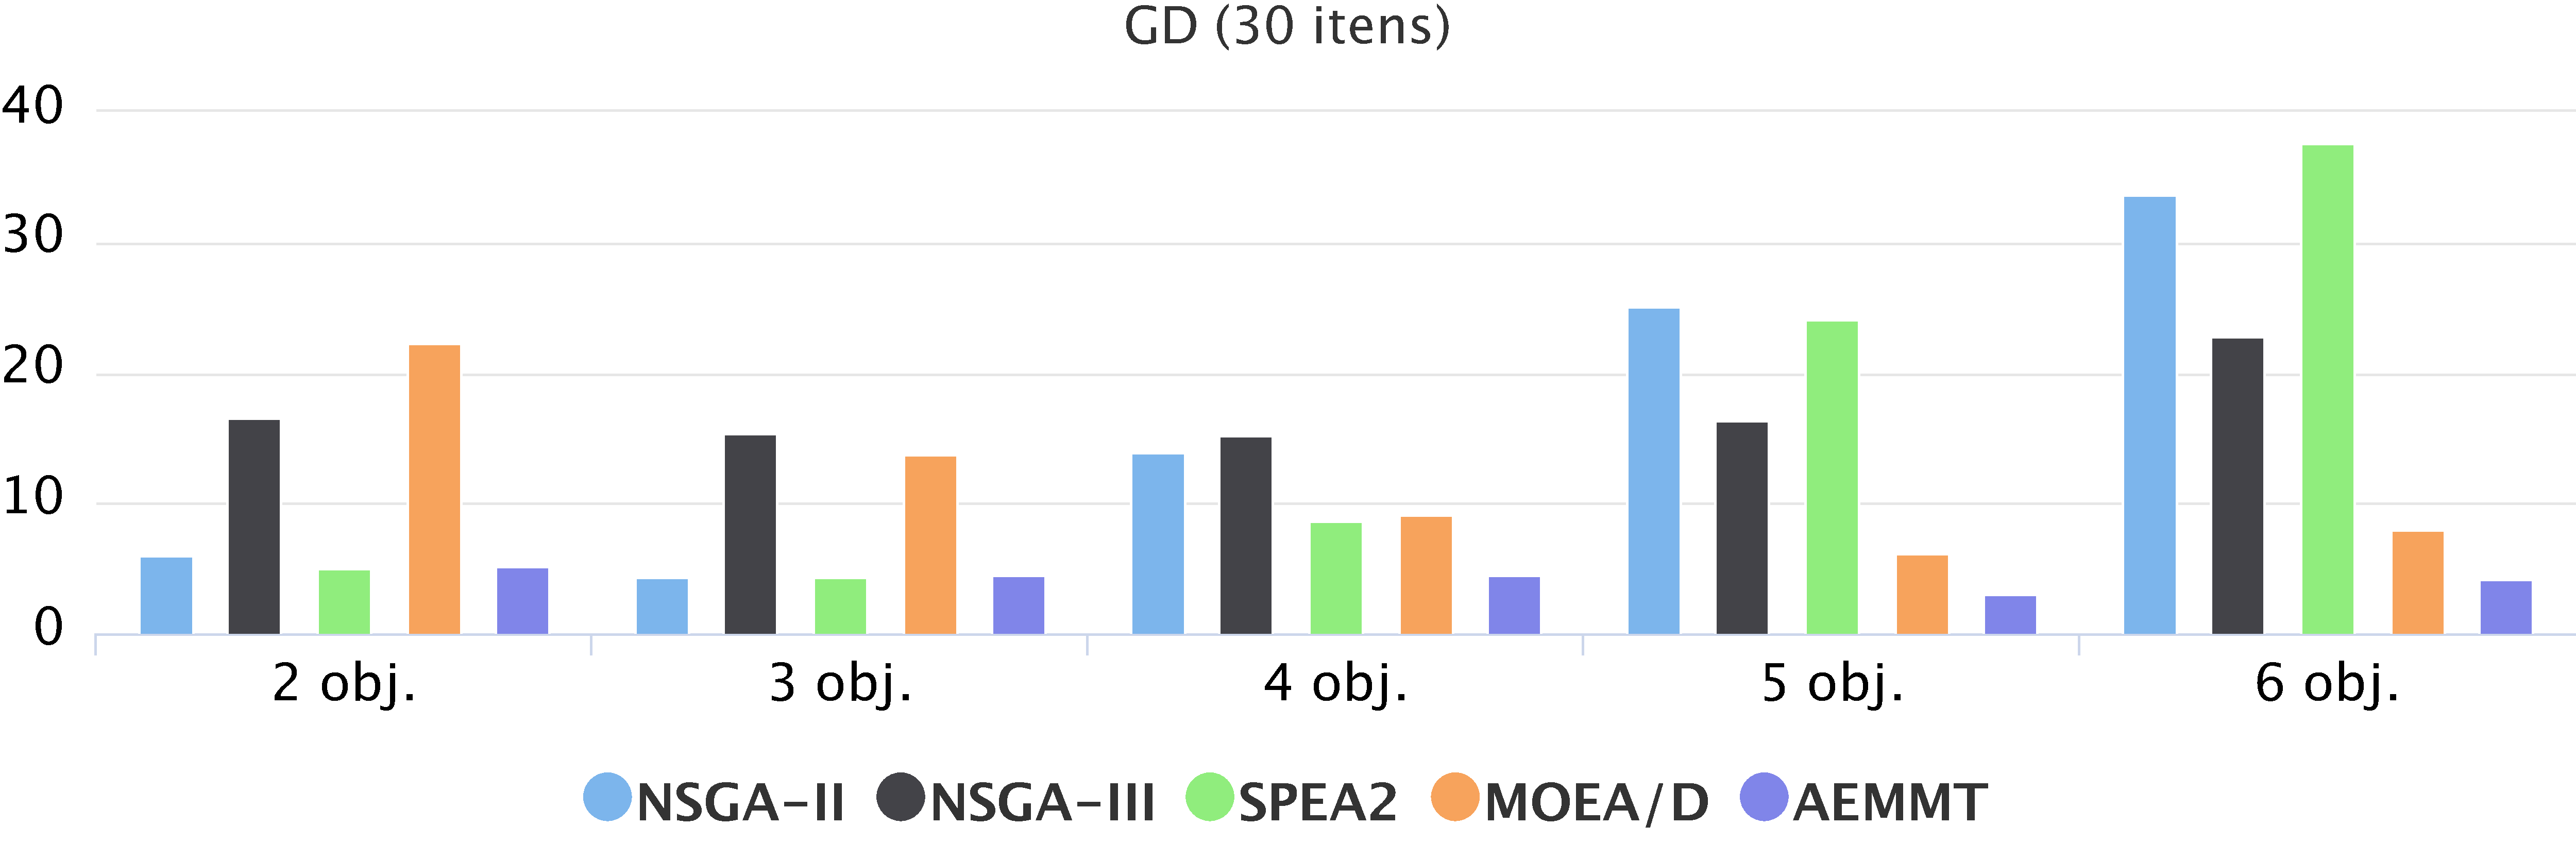
\includegraphics[width=1\textwidth]{cap_experimentos/figs/etapa1/gd-mkp-30}
	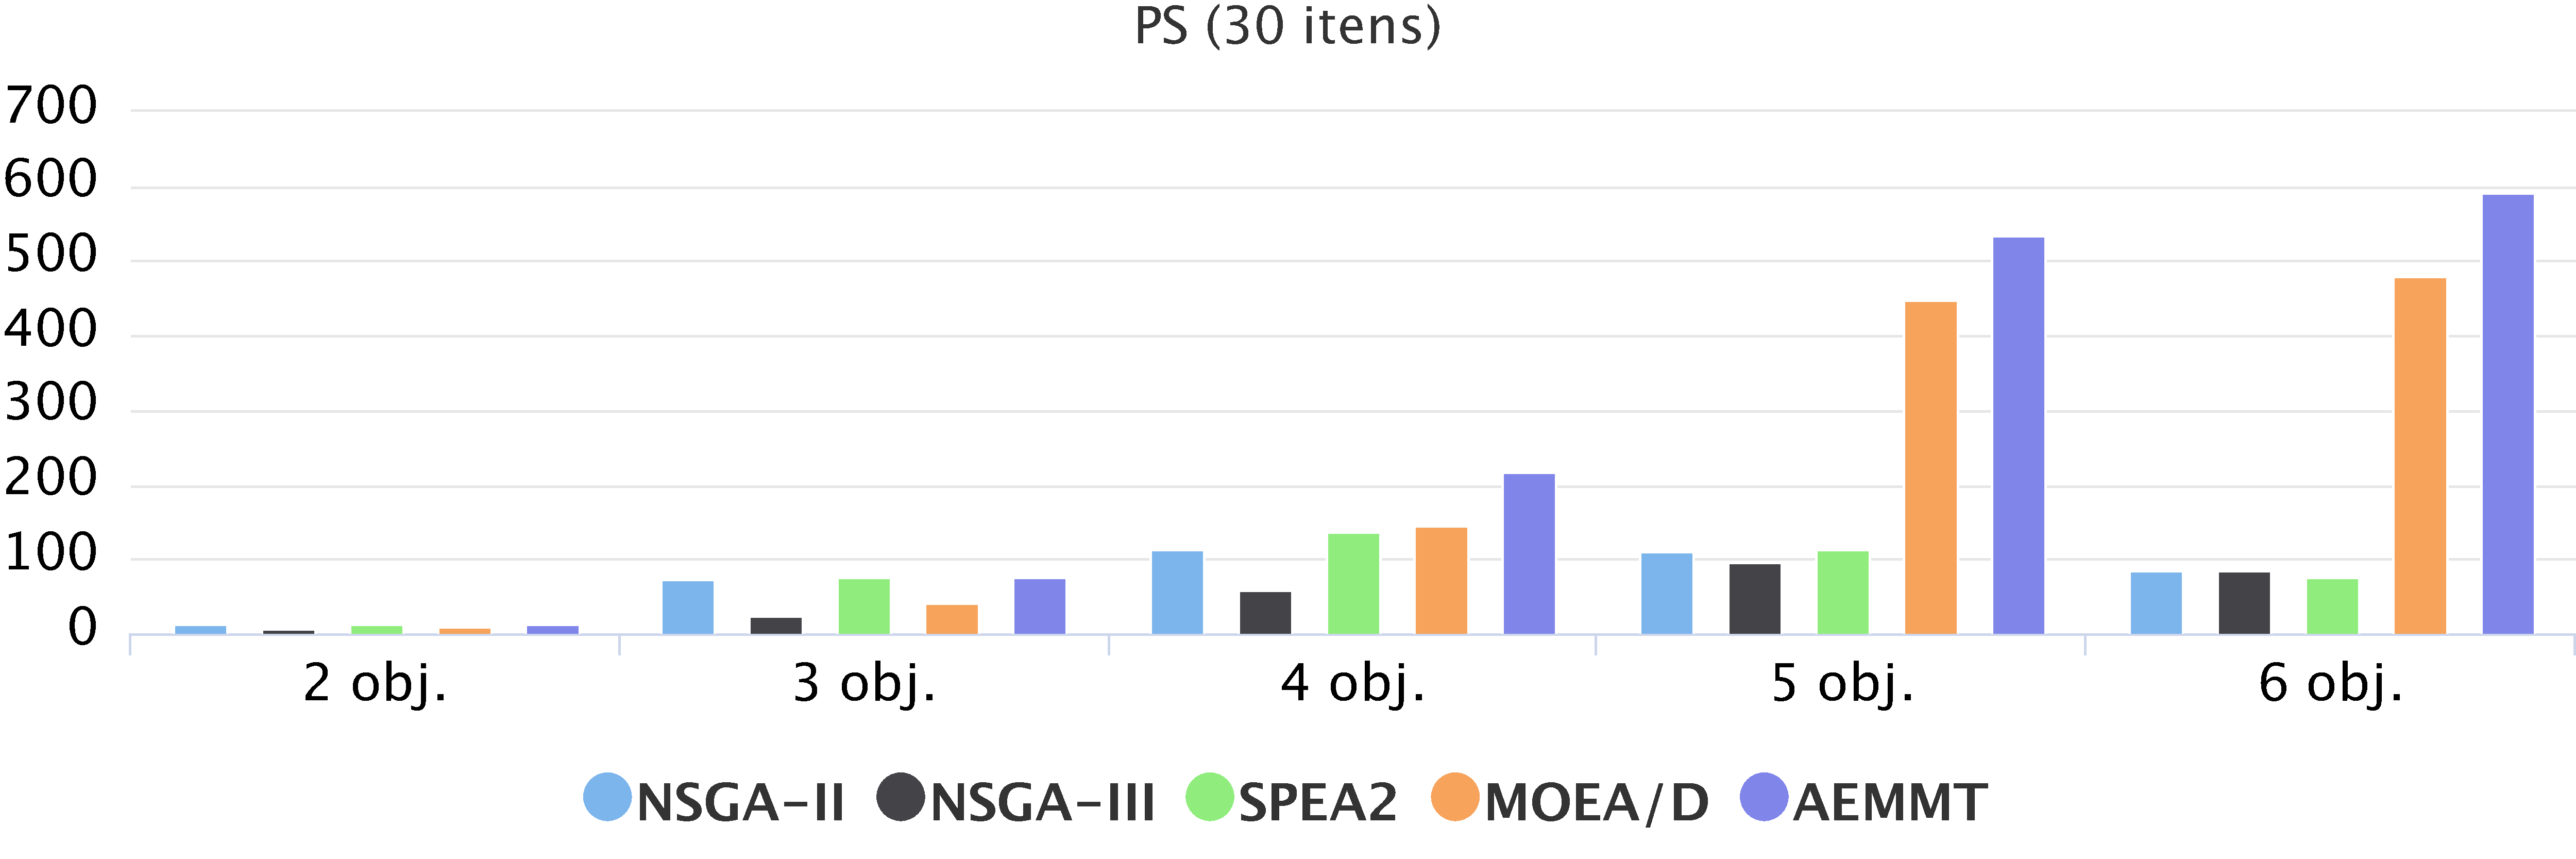
\includegraphics[width=1\textwidth]{cap_experimentos/figs/etapa1/ps-mkp-30}
	\caption{\label{fig_exp1_pmm_30}Desempenho dos algoritmos na 1ª etapa para o PMM com 30 itens}
\end{figure*}

Como pode ser observado na \autoref{fig_exp1_pmm_30}, o PMM com 30 itens é um problema relativamente simples e, no geral, os métodos de otimização multiobjetivo alcançam bons resultados. Até 4 objetivos, apenas o MOEA/D passou a marca de 20\% de erro. Para 2 e 3 objetivos, os algoritmos NSGA-II, SPEA2 e AEMMT apresentaram desempenhos muito similares, resultando nos melhores percentuais de erro entre todos os algoritmos avaliados. A partir de 4 objetivos é possível notar uma queda considerável no desempenho dos algoritmos multiobjetivos clássicos (NSGA-II e SPEA-2). Considerando-se todas as formulações de objetivo no PMM, os melhores resultados foram obtidos pelo AEMMT que manteve o erro abaixo de 6\% em todos os casos. Analisando a métrica $GD$, obtêm-se as mesmas conclusões tiradas a partir do $ER$. Isto é, considerando todas as formulações, o AEMMT gera os melhores resultados. Por outro lado, apesar de terem um desempenho muito bom nos problemas de 2 e 3 objetivos, os valores da métrica GD para o NSGA-II e o SPEA2 apresentam resultados ruins a partir de 4 objetivos. O tamanho da fronteira de Pareto encontrada, medida pelo $PS$, é maior nos algoritmos MOEA/D e AEMMT. Esse comportamento é esperado, pois diferentemente dos demais AEMOs, esses dois algoritmos não aplicam uma limitação sobre o tamanho do arquivo que armazena as soluções não-dominadas. Considerando-se os valores das três métricas em todas as formulações de objetivos para o PMM de 30 itens, está claro que, no geral, o AEMMT é o melhor dentre os métodos testados.

\begin{figure*}[!htbp]
	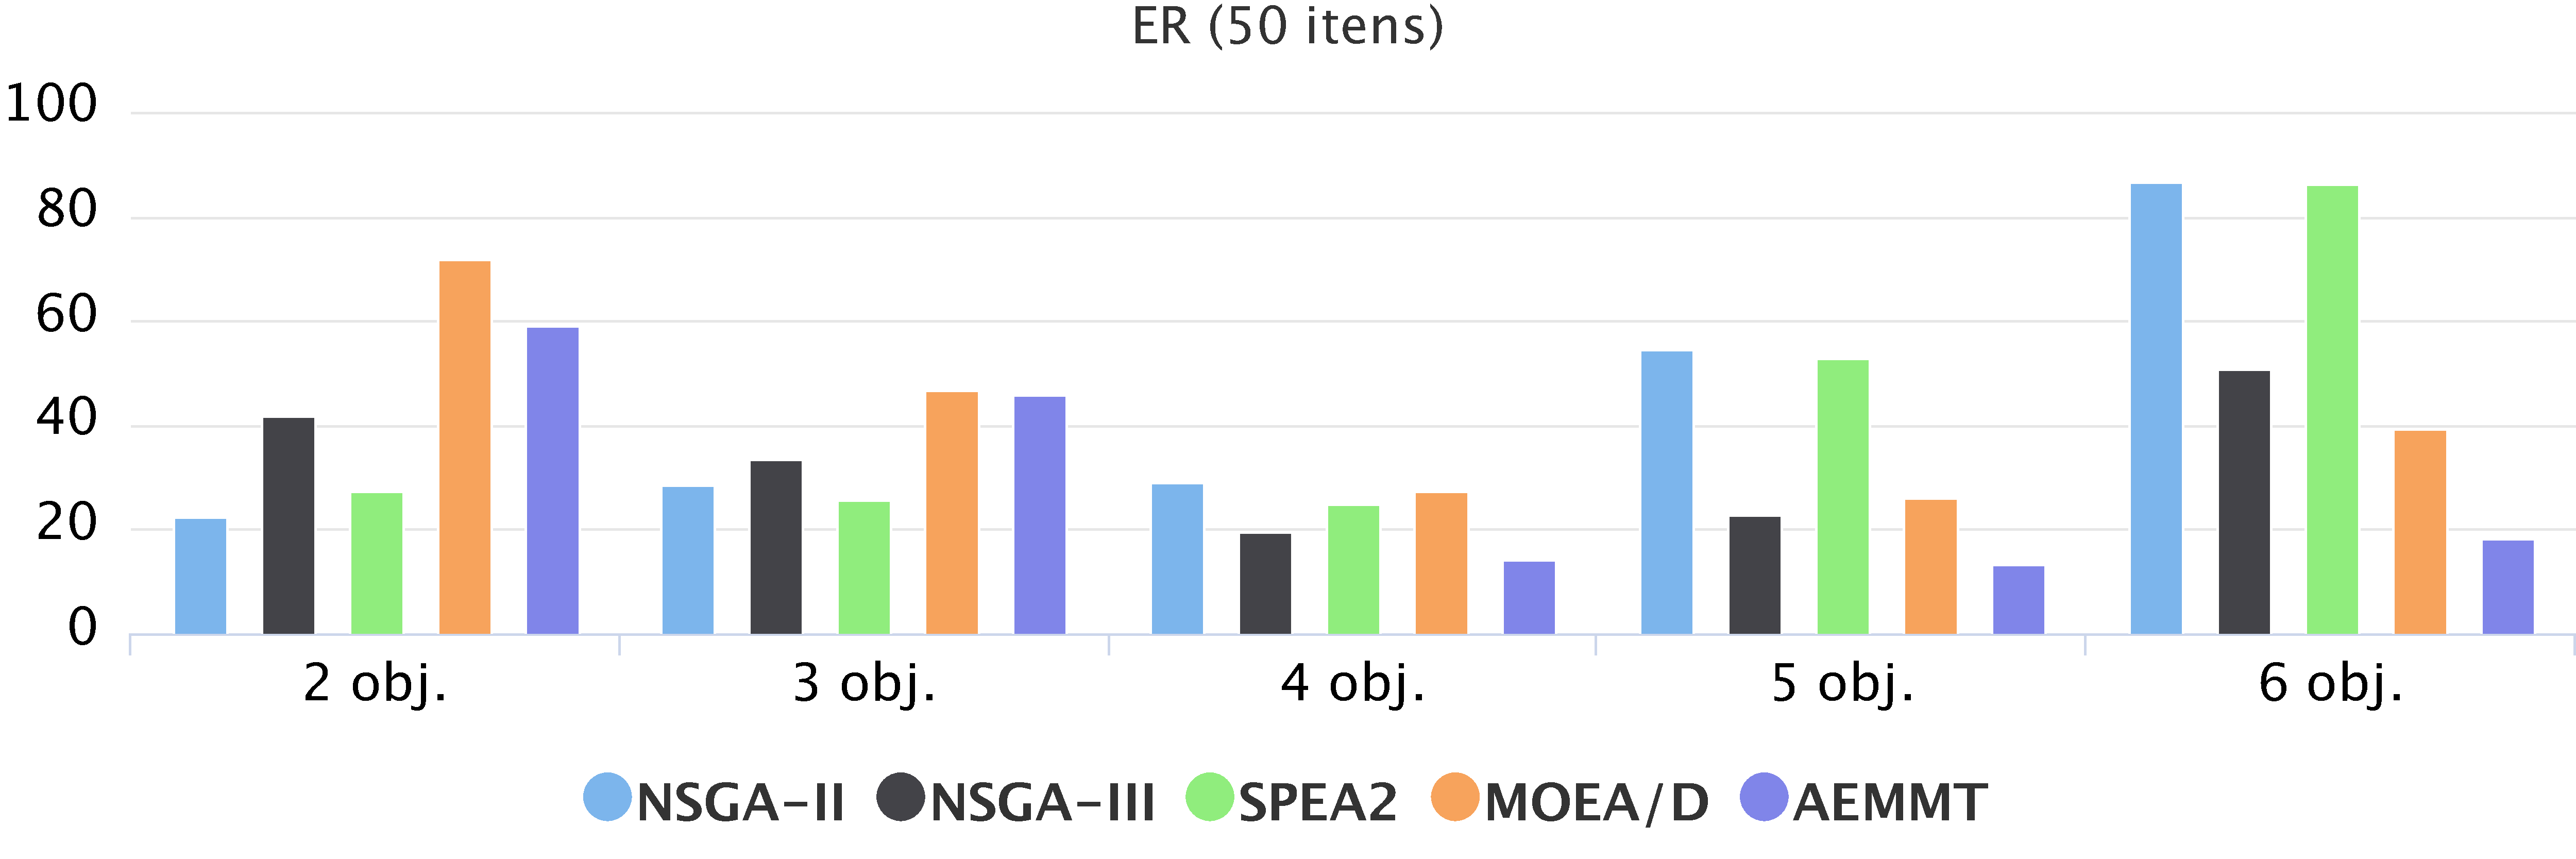
\includegraphics[width=1\textwidth]{cap_experimentos/figs/etapa1/er-mkp-50}
	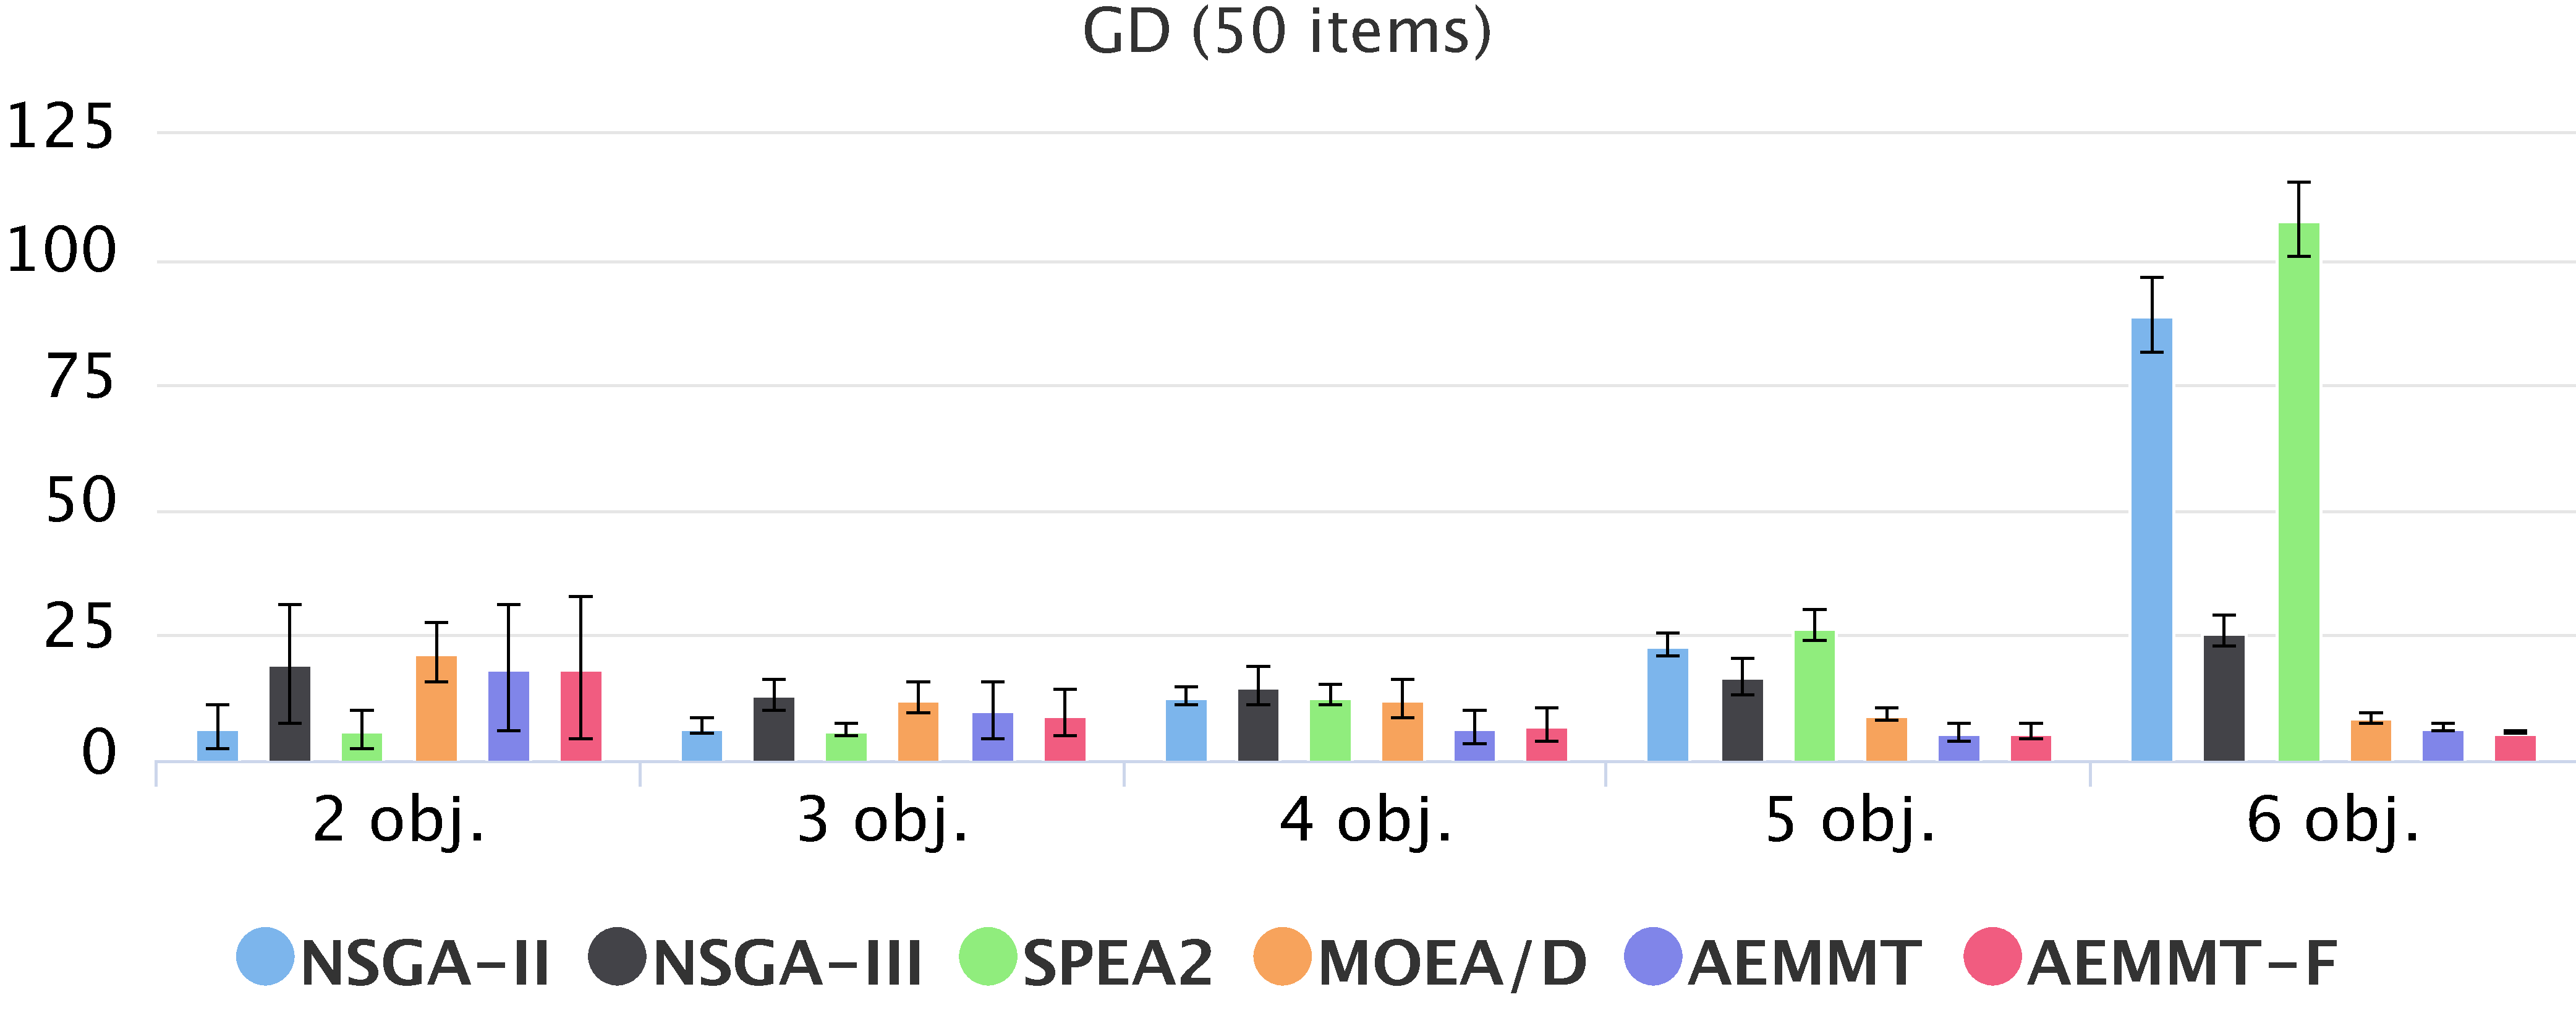
\includegraphics[width=1\textwidth]{cap_experimentos/figs/etapa1/gd-mkp-50}
	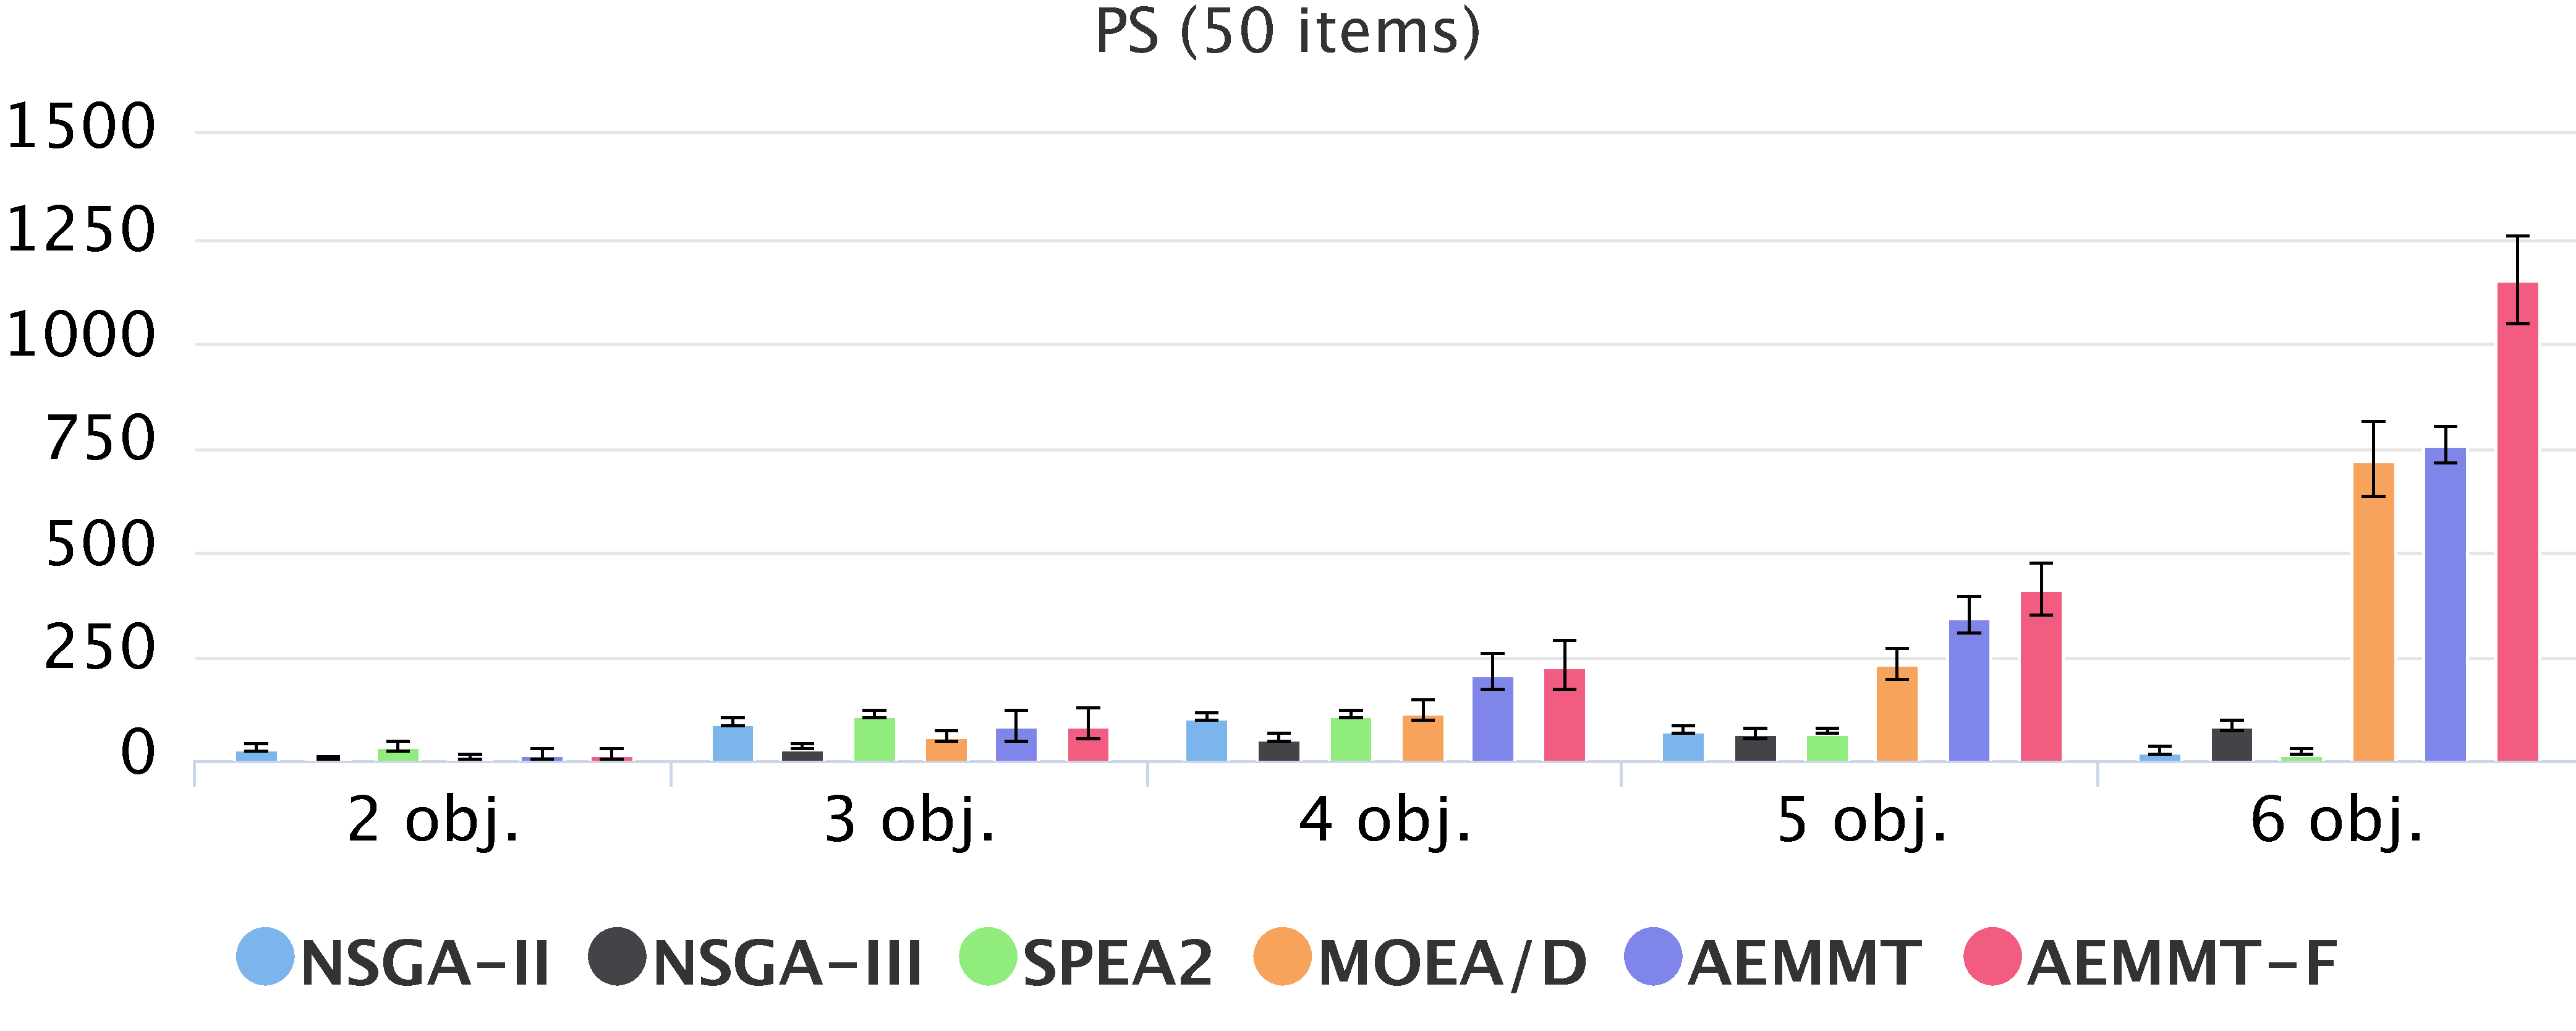
\includegraphics[width=1\textwidth]{cap_experimentos/figs/etapa1/ps-mkp-50}
	\caption{\label{fig_exp1_pmm_50}Desempenho dos algoritmos na 1ª etapa para o PMM com 50 itens}
\end{figure*}

O PMM com 50 itens (\autoref{fig_exp1_pmm_50}) é um problema mais complexo que sua versão com 30 itens e os algoritmos têm mais dificuldade para convergir para o Pareto aproximado, o que pode ser comprovado pelas taxas de erro maiores em relação ao experimento anterior. Nessa instância, é mais evidente  o comportamento de cada algoritmo em função das diferentes formulações de objetivos. Nas formulações com 2 e 3 objetivos, os algoritmos clássicos (NSGA-II e SPEA2) são imbatíveis, independentemente da métrica analisada. A partir de 4 objetivos, o AEMMT assume a primeira posição e é o melhor algoritmo tanto para $ER$ quanto para $GD$ e $PS$. Depois do AEMMT, para 4 objetivos, a menor taxa de erro é atingida pelo NSGA-III, seguido pelos SPEA2, MOEA/D e NSGA-II. Para 5 objetivos, o NSGA-III continua apresentando a segunda menor taxa de erro, enquanto o MOEA/D obtém resultado melhor que o SPEA2. Para seis objetivos, o MOEA/D tem $ER$ pior apenas que o AEMMT e o NSGA-III apresenta o terceiro melhor resultado. Com relação ao $GD$, o MOEA/D obtém o segundo melhor desempenho para as formulações \textit{many-objective} (a partir de 4 objetivos) e o NSGA-III obtém o terceiro melhor, excluindo a formulação com 4 objetivos, onde o SPEA2 é melhor. O $PS$, a partir de 4 objetivos, é dominado pelos algoritmos AEMMT e MOEA/D, o NSGA-III possui um comportamento mais parecido com os algoritmos clássicos que com os algoritmos \textit{many-objective}.  É possível notar que, com o aumento do número de objetivos, o NSGA-II e o SPEA2 pioram enquanto o AEMMT mantém o $ER$ e o $GD$ estáveis e melhora o $PS$. O MOEA/D é o segundo melhor algoritmo para problemas \textit{many-objectives} e o NSGA-III é o terceiro. Para o PMM de 50 itens, o AEMMT é a melhor opção para muitos objetivos, assim como observado no PMM com 30 itens.

\begin{figure*}[!htbp]
	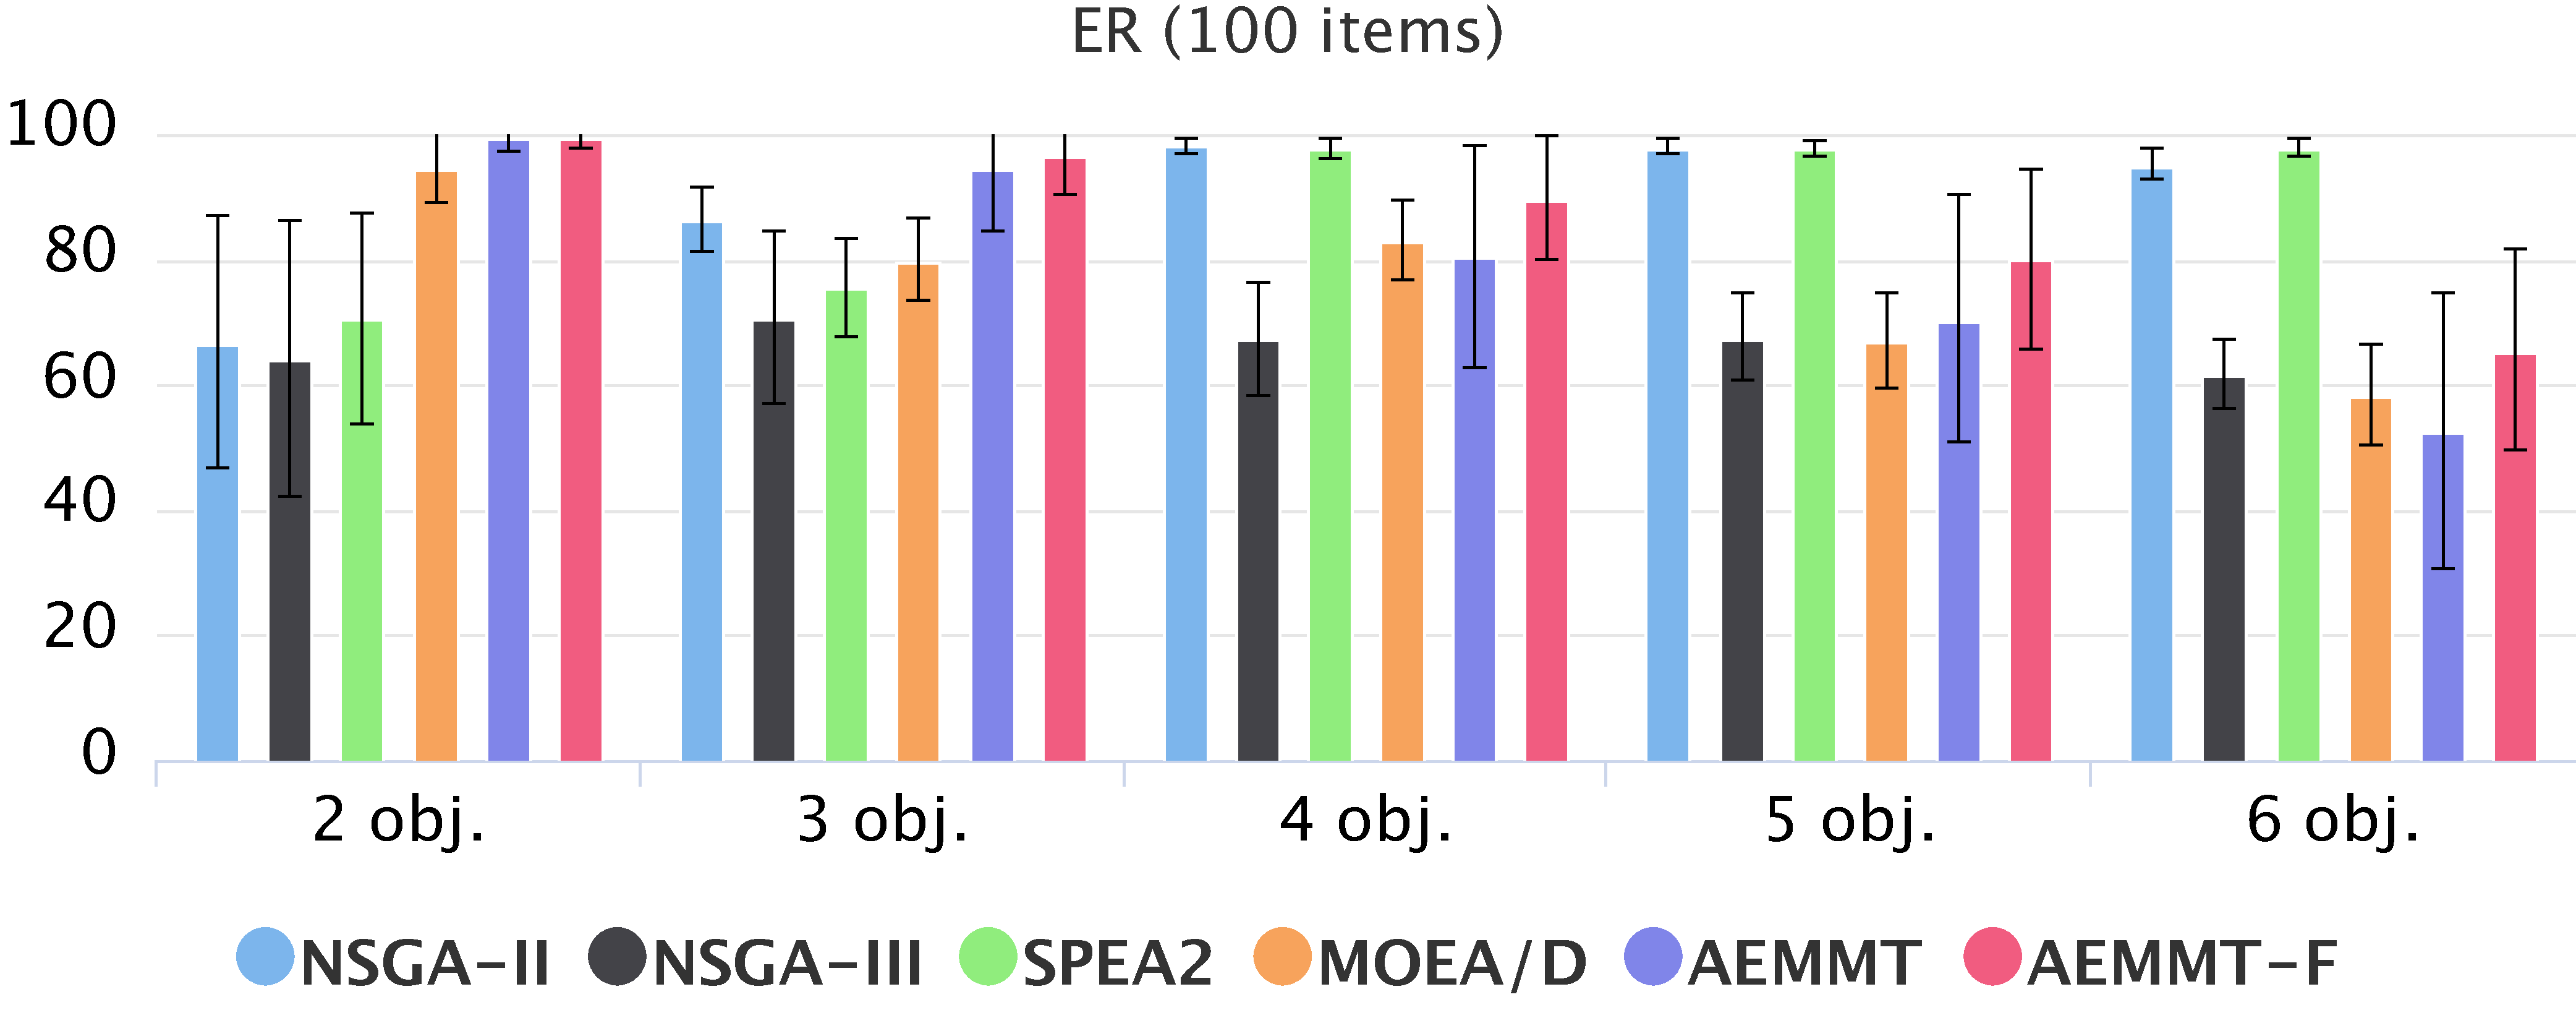
\includegraphics[width=1\textwidth]{cap_experimentos/figs/etapa1/er-mkp-100}
	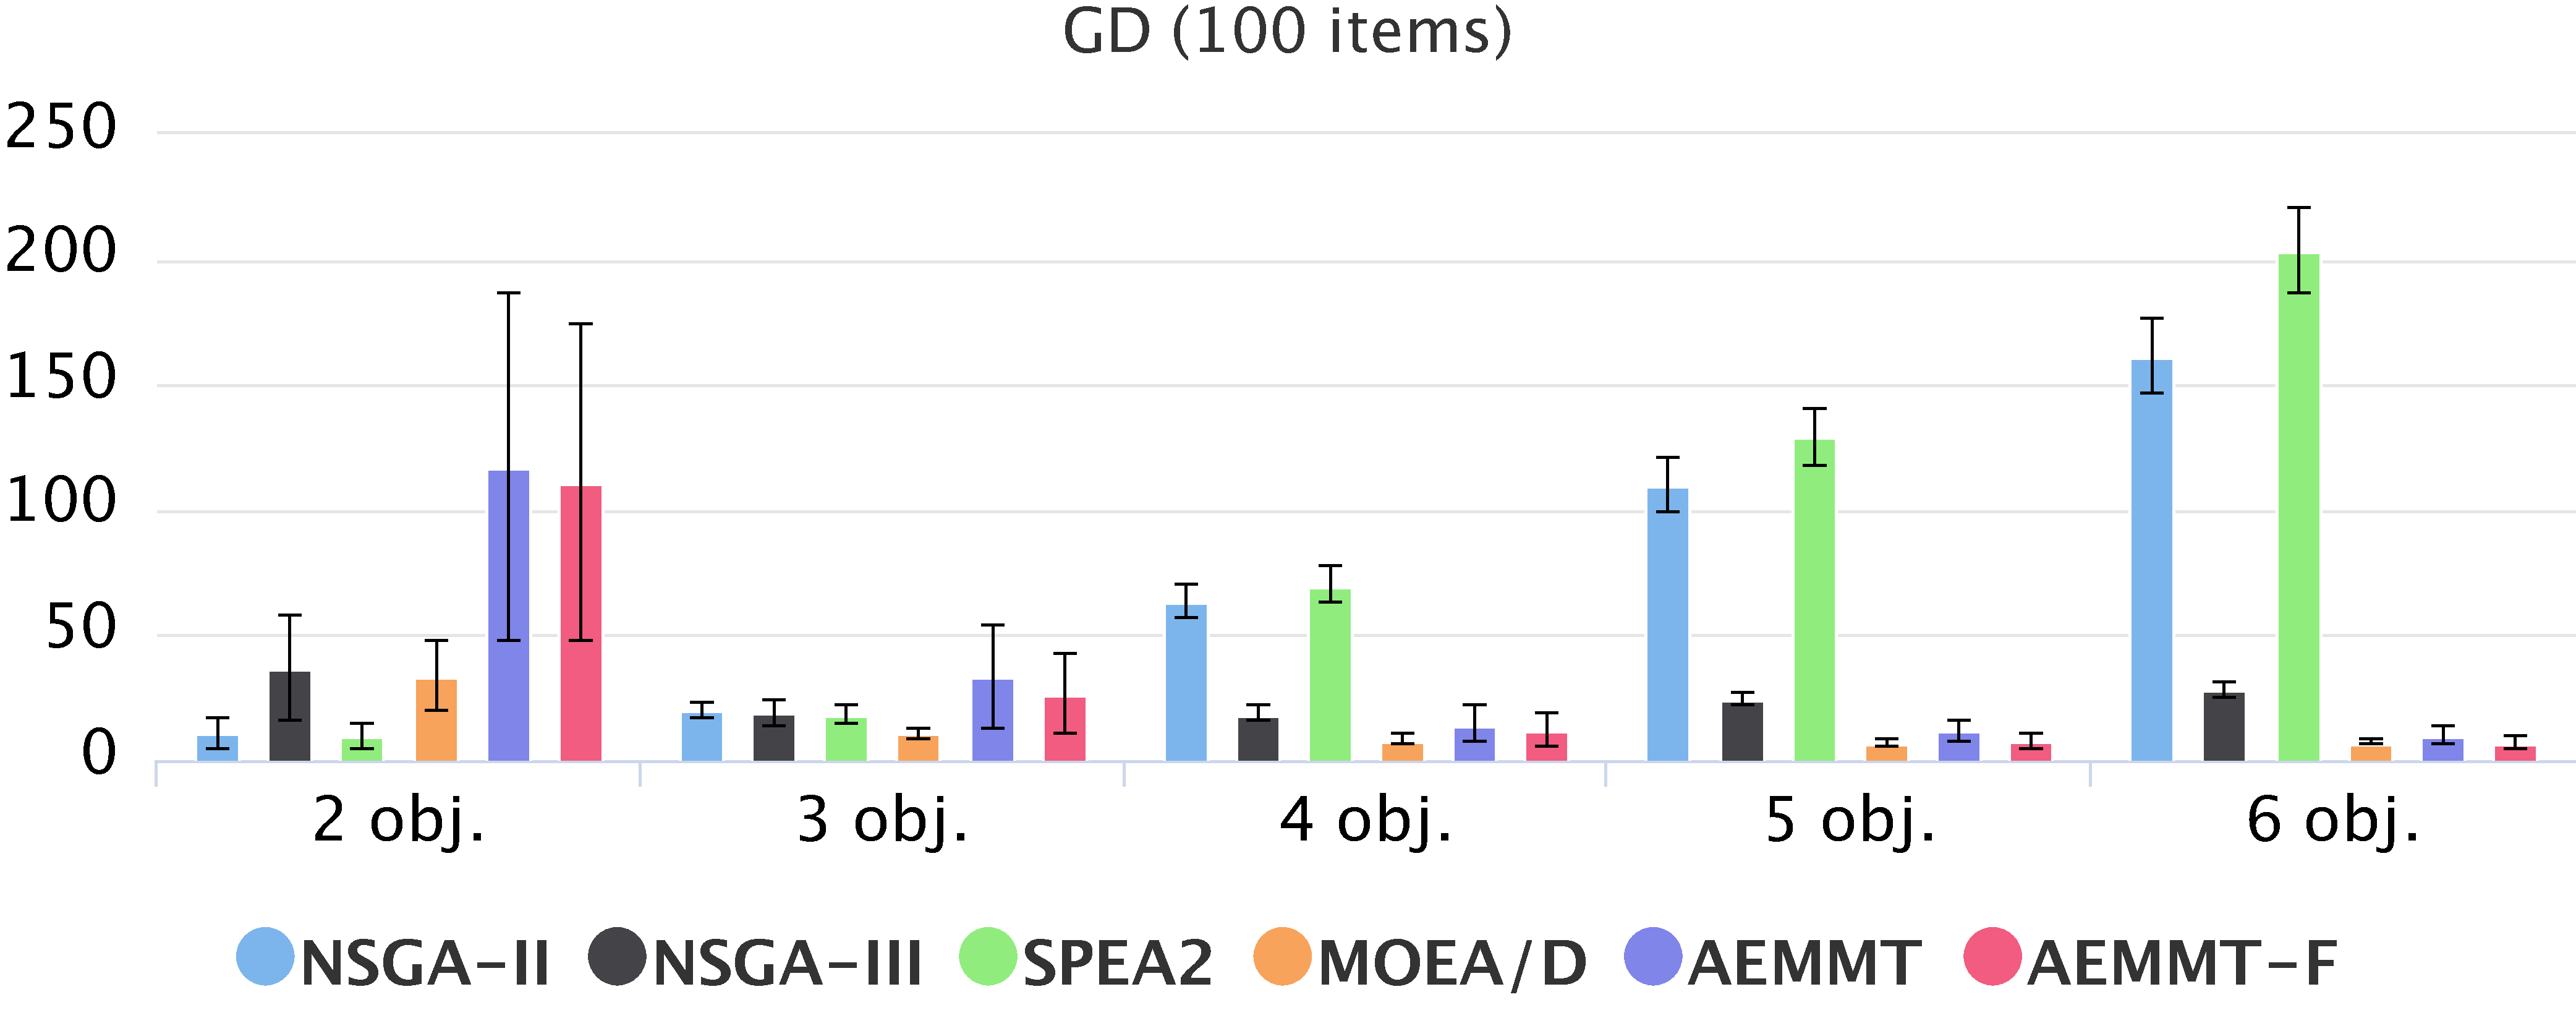
\includegraphics[width=1\textwidth]{cap_experimentos/figs/etapa1/gd-mkp-100}
	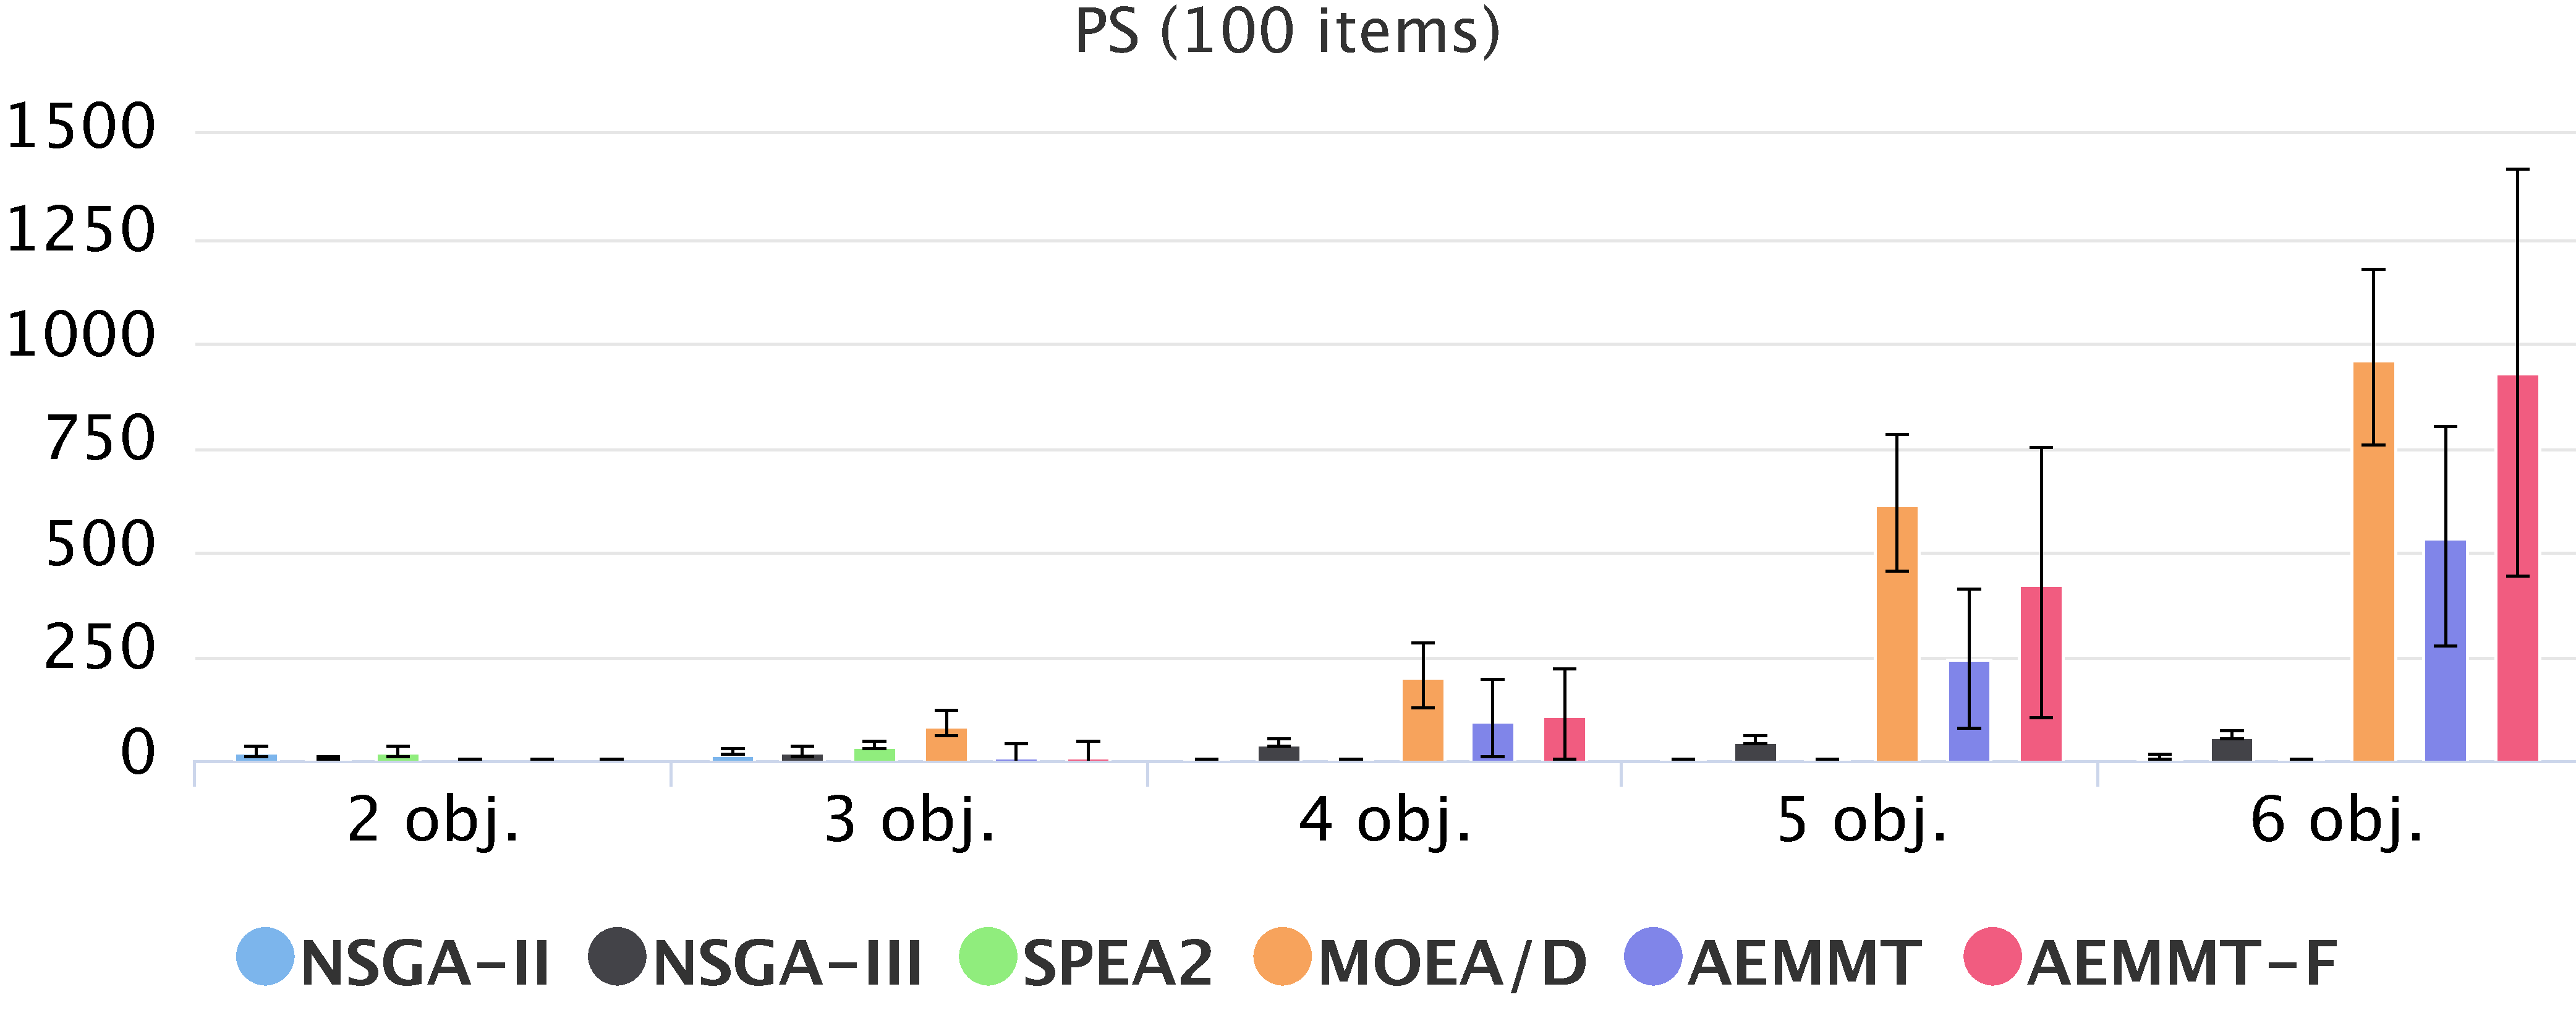
\includegraphics[width=1\textwidth]{cap_experimentos/figs/etapa1/ps-mkp-100}
	\caption{\label{fig_exp1_pmm_100}Desempenho dos algoritmos na 1ª etapa para o PMM com 100 itens}
\end{figure*}

O tamanho do espaço de busca no problema da mochila é $2^n$, sendo $n$ o número de itens. Portanto, a complexidade do PMM com 100 itens, cujos resultados são apresentados na \autoref{fig_exp1_pmm_100}, é muito maior que nas instâncias anteriores. Nesse caso, não foi possível encontrar um Pareto estável para as formulações de 4, 5 e 6 objetivos. Dessa forma, apesar de as métricas $ER$, $GD$ e $PS$ serem um bom indicativo do desempenho entre os algoritmos, a melhor forma de avaliação seria o hipervolume. Um experimento similar, mas utilizando o hipervolume, é apresentado na Seção \ref{section_experimentos_etapa4}. É difícil avaliar o problema considerando 100 itens, pois, a partir dos resultados apresentados para a métrica de erro (ER) na \autoref{fig_exp1_pmm_100}, é possível perceber que poucos algoritmos conseguiram encontrar boas soluções. Considerando a métrica $ER$, o algoritmo com melhor desempenho retornou uma taxa de erro acima de 50\%. O NSGA-III apresentou o menor $ER$ nos cenários de 2, 3, 4 e 5 objetivos, enquanto que na formulação de 6, os melhores desempenhos nessa métrica foram obtidos pelos AEMMT e MOEA/D. Com relação ao $GD$, o NSGA-II e o SPEA2 apresentaram os melhores resultados para 2 objetivos. Na formulação de 3 objetivos em diante, o MOEA/D foi o algoritmo com menor $GD$, sendo que , a partir de 4 objetivos, o AEMMT obteve desempenho similar. A situação se repete ao analisar o $PS$. A partir de 3 objetivos, o MOEA/D traz um conjunto maior de soluções na fronteira de Pareto, seguido pelo AEMMT a partir de 4 objetivos. Em problemas com muitos objetivos, o AEMMT e o MOEA/D são as melhores opções, sendo que o AEMMT apresenta uma taxa de erro levemente menor e o MOEA/D obtém um valor de $PS$ consideravelmente melhor. Para problemas com 4 objetivos ou menos, o NSGA-III é o método que consegue as soluções mais próximas do Pareto. Entretanto, o conjunto de soluções gerado pelo NSGA-III não é tão grande quanto aquele gerado pelo MOEA/D. Conforme ressaltado anteriormente, o NSGA-III possui um limite no número de soluções não-dominadas possíveis de serem encontradas, diferentemente do AEMMT e do MOEA/D, que é o próprio tamanho da população. Entretanto, é possível observar que o tamanho de $PS$ obtido pelo NSGA-III é abaixo desse limite (150).

\begin{figure*}[!htbp]
	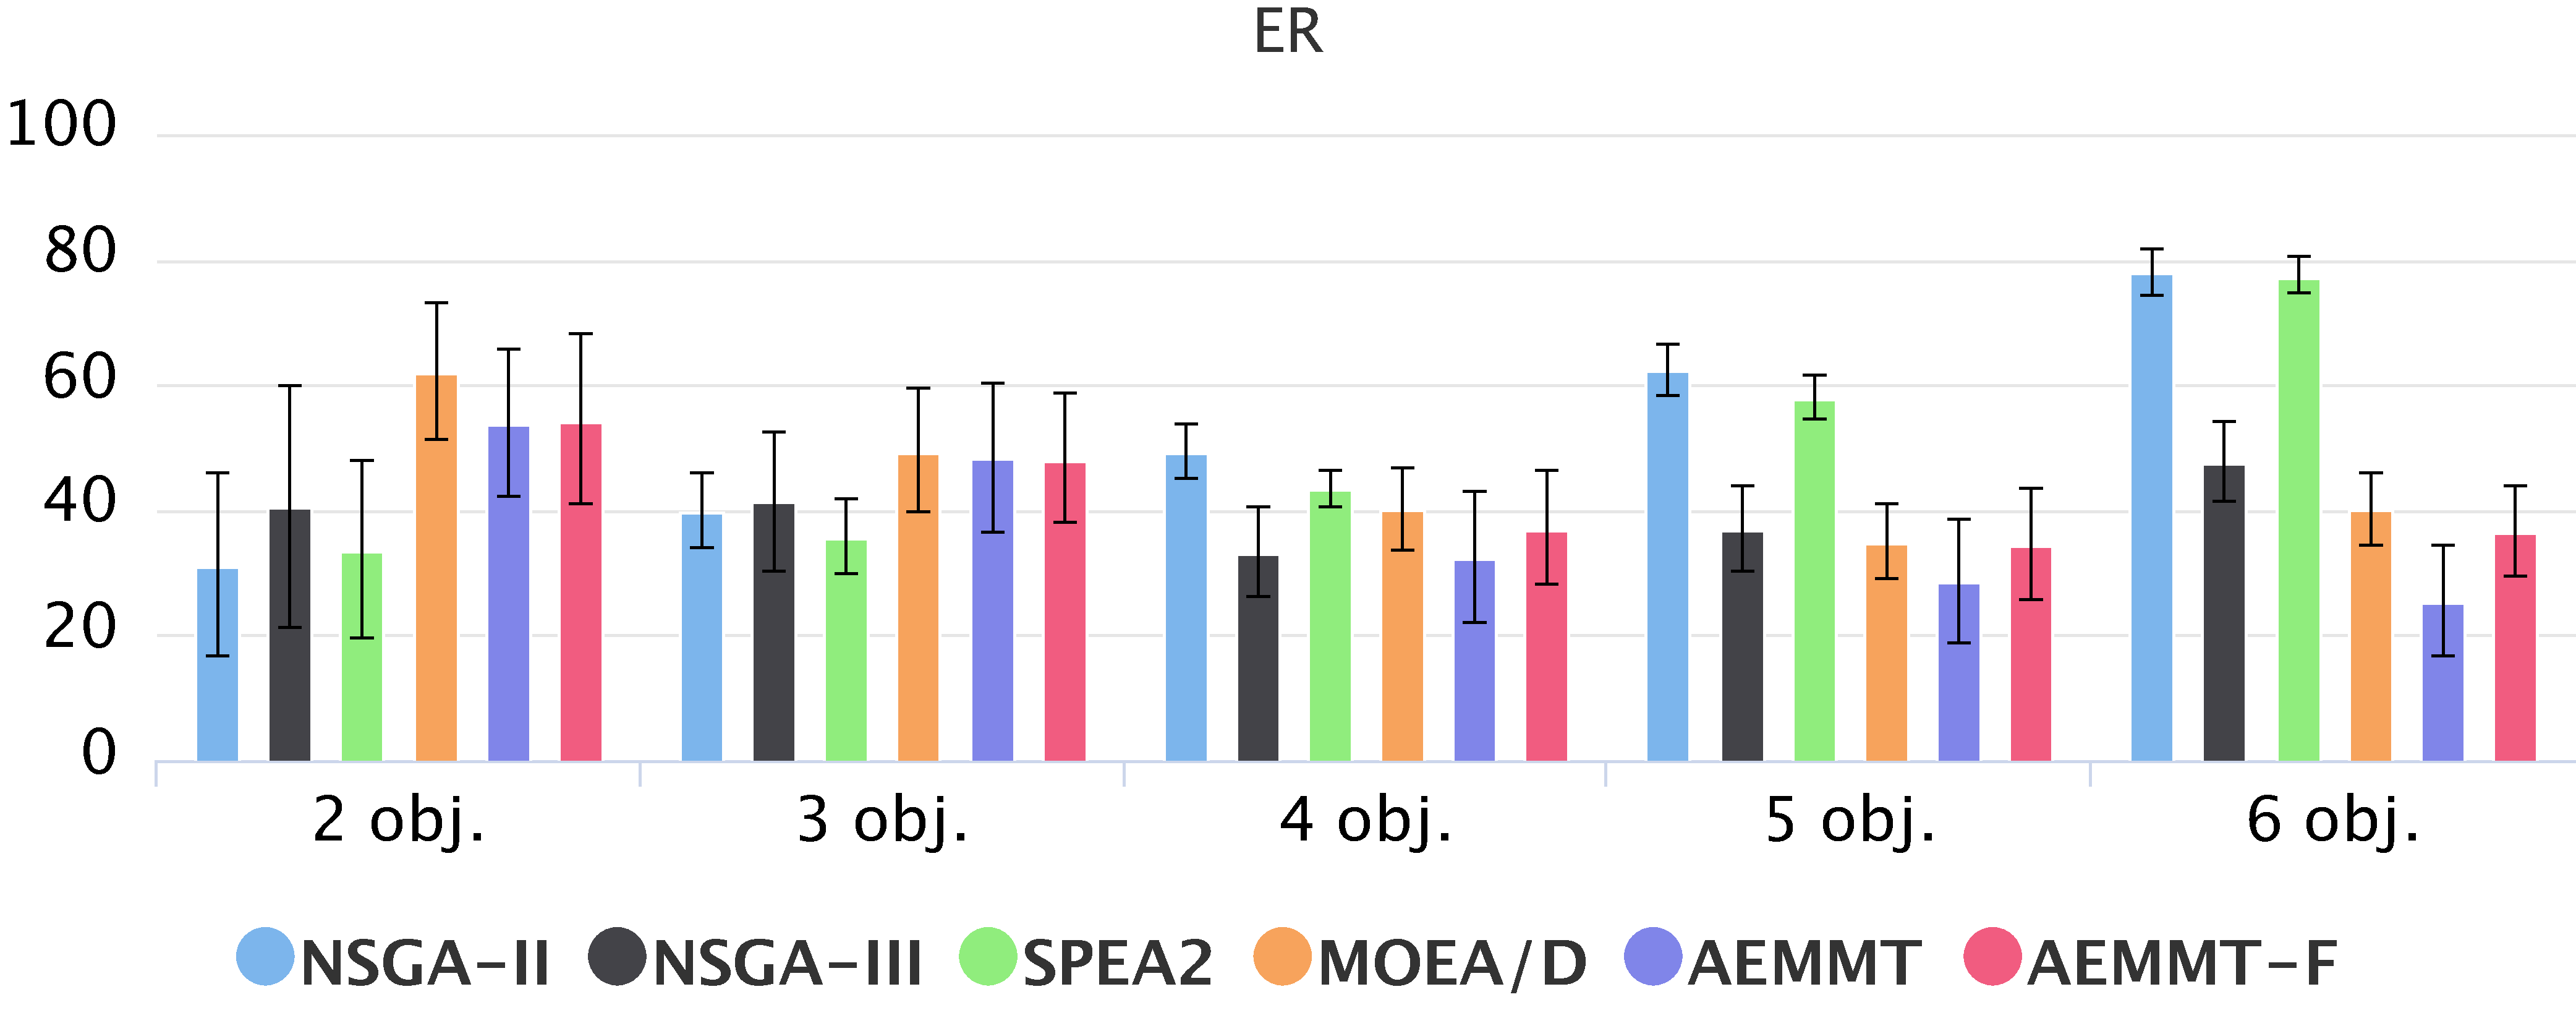
\includegraphics[width=1\textwidth]{cap_experimentos/figs/etapa1/er-mkp-todos}
	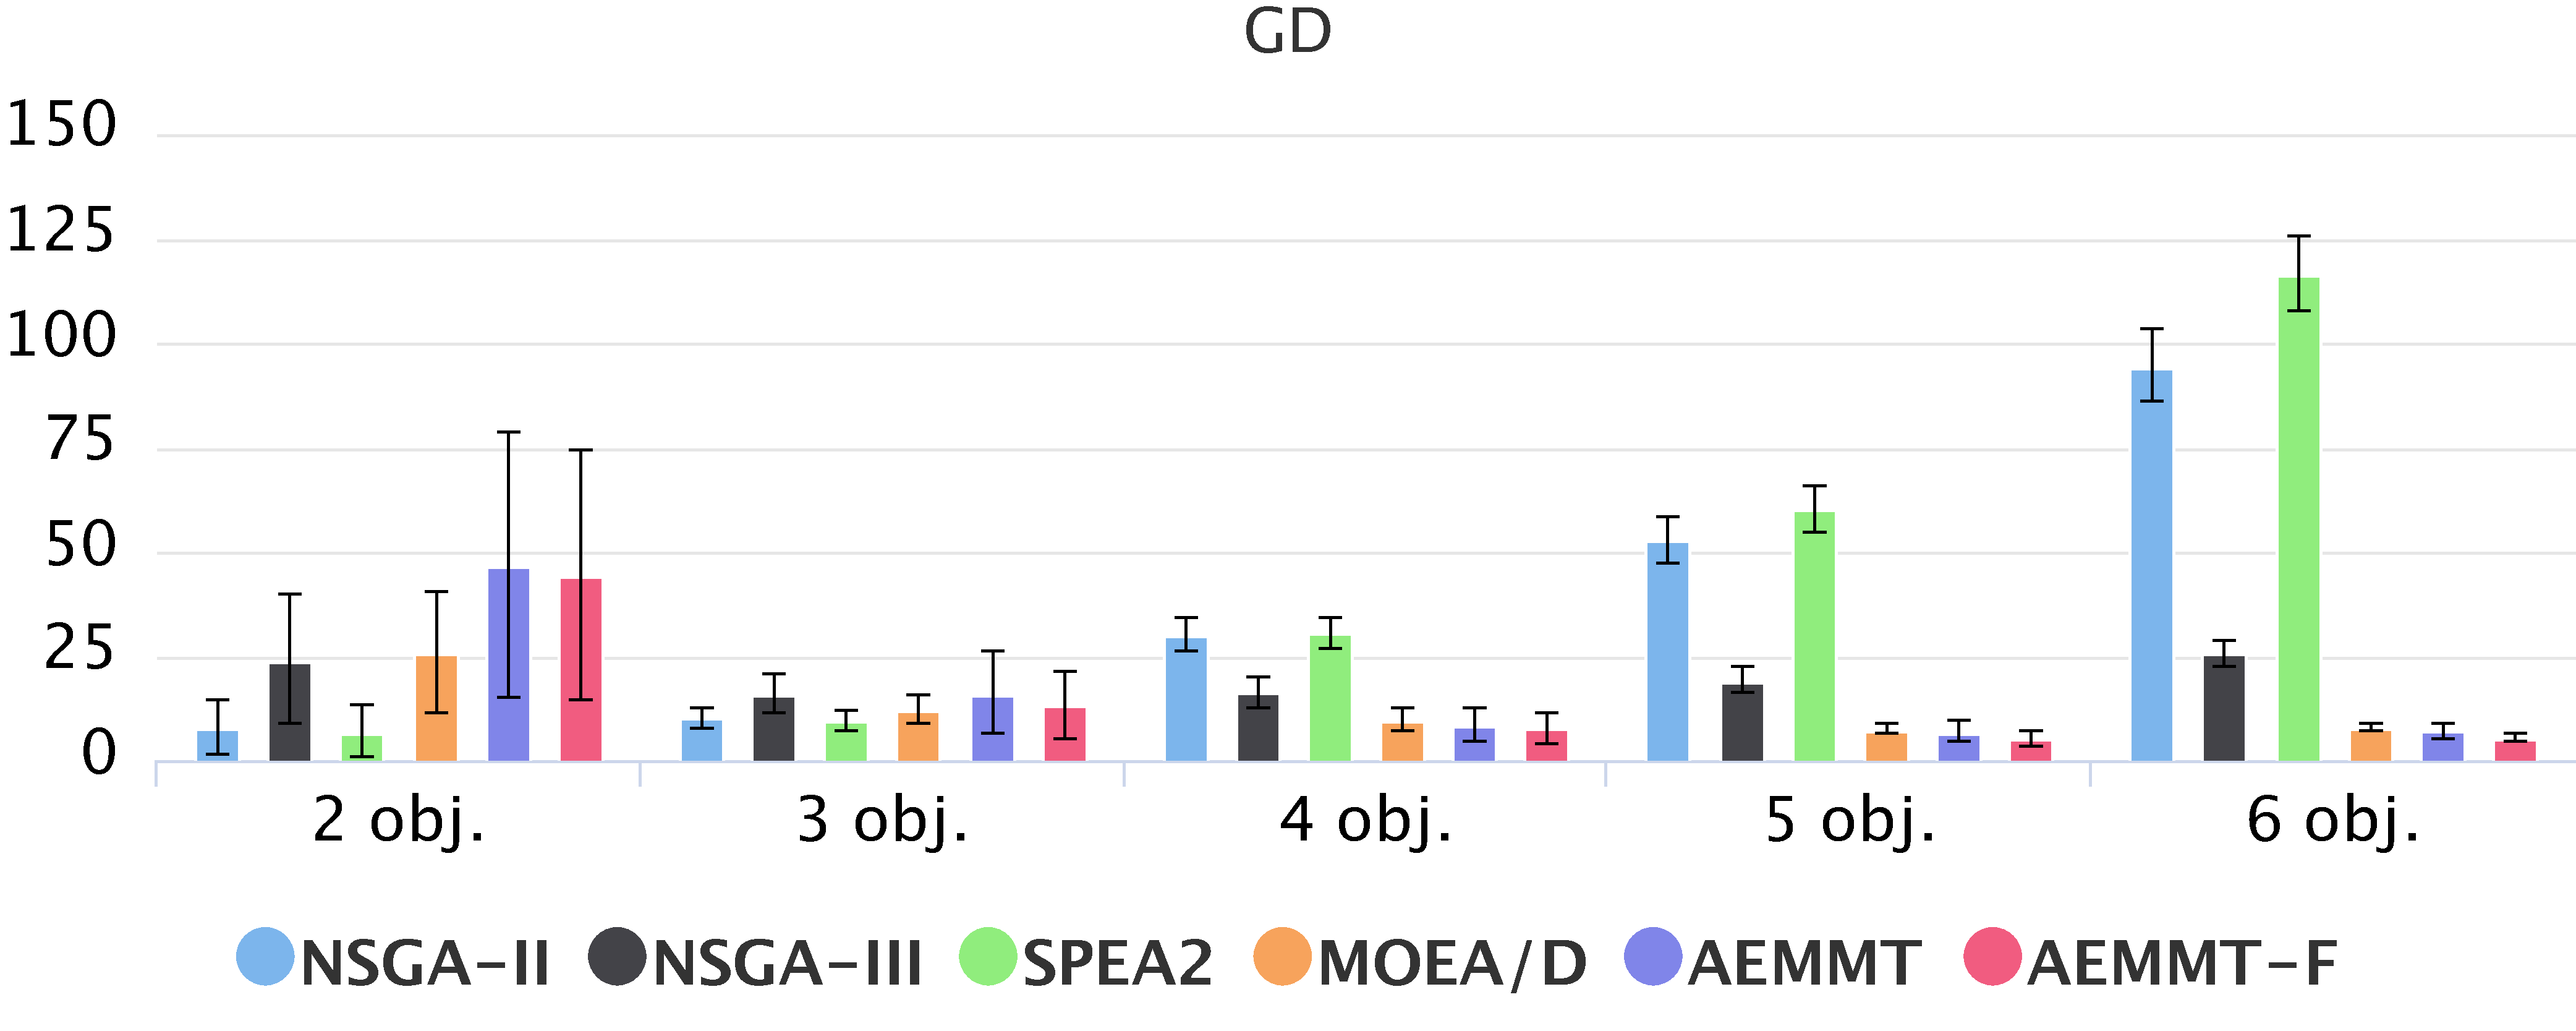
\includegraphics[width=1\textwidth]{cap_experimentos/figs/etapa1/gd-mkp-todos}
	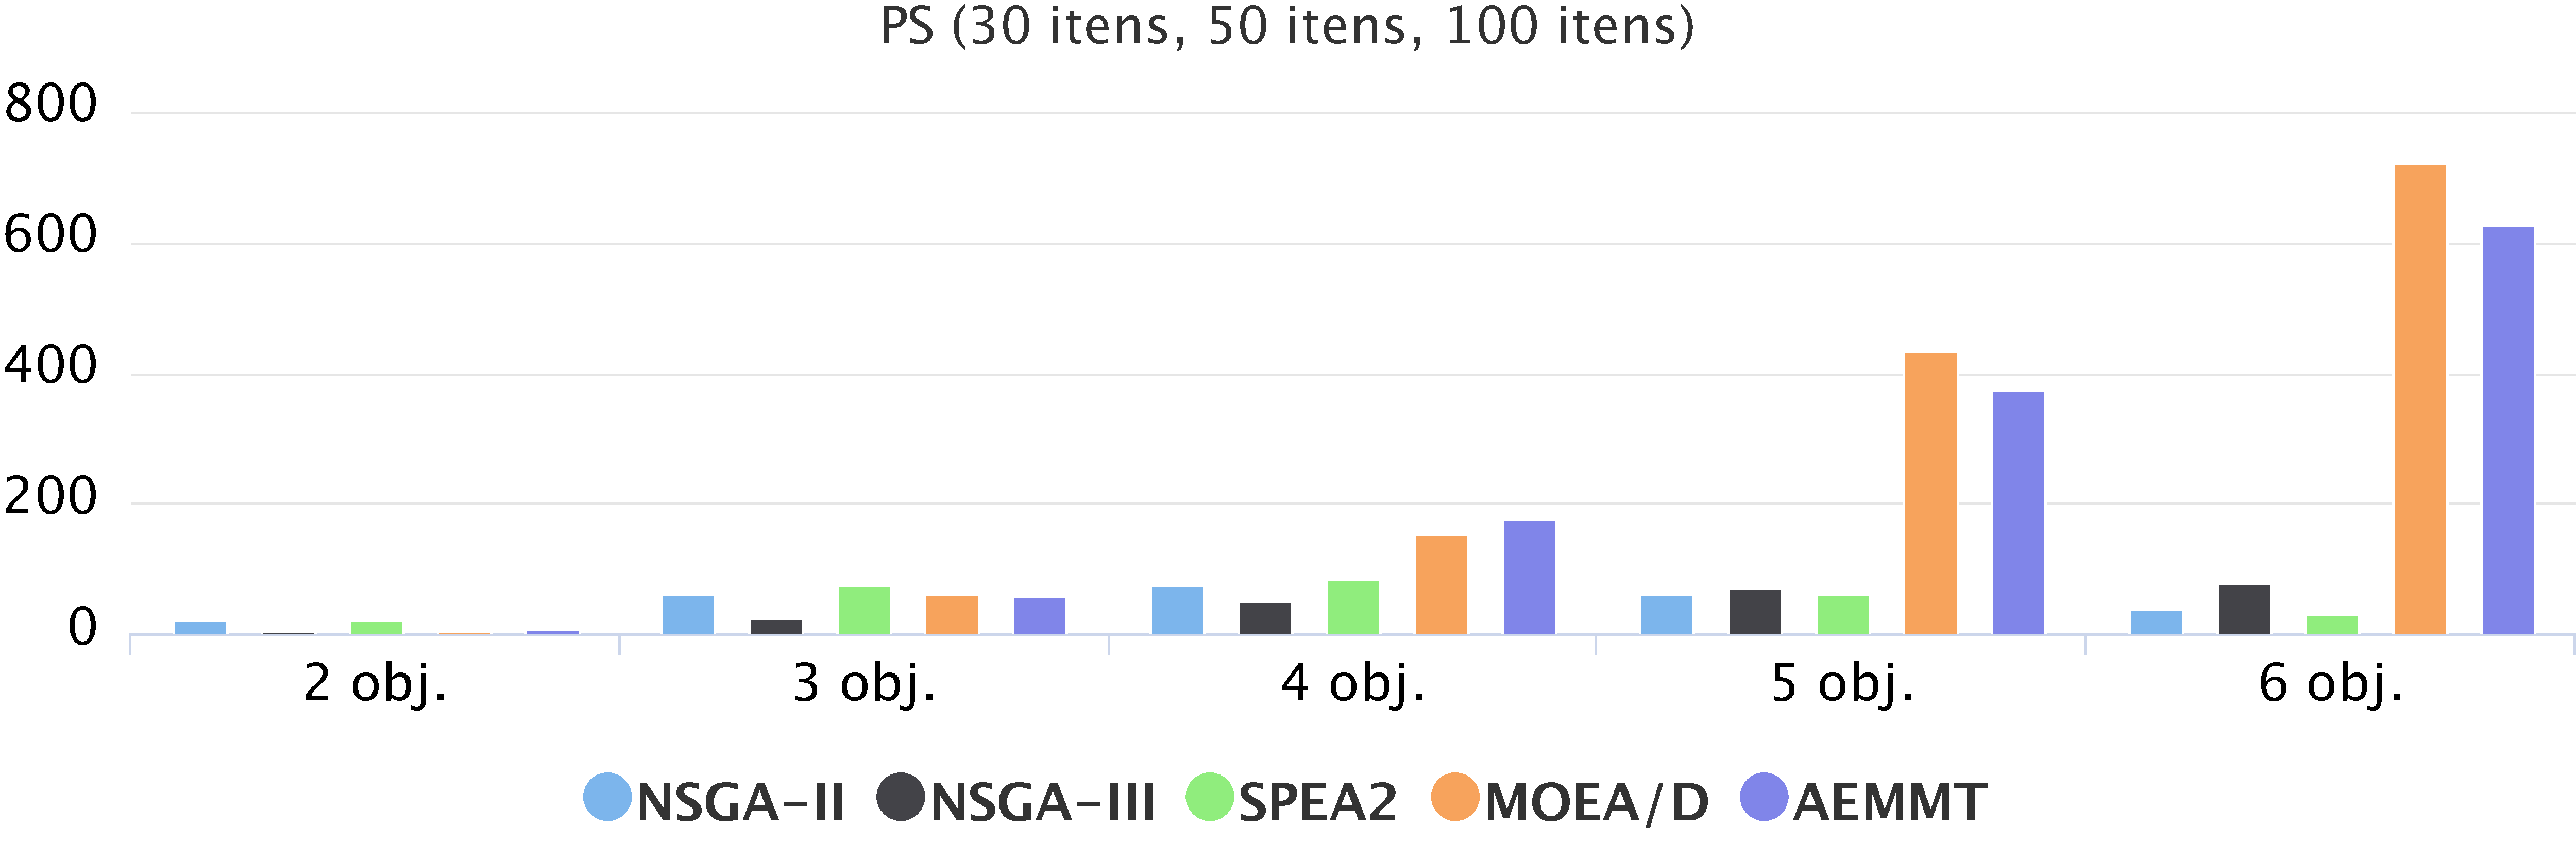
\includegraphics[width=1\textwidth]{cap_experimentos/figs/etapa1/ps-mkp-todos}
	\caption{\label{fig_exp1_pmm_todos}Resultado consolidado da 1ª etapa considerando o PMM com 30, 50 e 100 itens}
\end{figure*}

A \autoref{fig_exp1_pmm_todos} apresenta os resultados do PMM de 30, 50 e 100 itens de forma consolidada para que se possa analisar, de forma geral, o comportamento dos algoritmos nas diferentes formulações de objetivo. Os gráficos representam as médias (simples) entre os três cenários de dificuldade (30, 50 e 100 itens). Como esperado, o NSGA-II e o SPEA2 são os melhores algoritmos para as formulações de 2 e 3 objetivos, tendo resultado nos melhores valores para as métricas $ER$, $GD$ e $PS$. Por outro lado, a partir de 4 objetivos, o desempenho de ambos os algoritmos cai consideravelmente, enquanto o AEMMT passa a apresentar os melhores resultados. O NSGA-III, no problema de 4 objetivos, apresenta um erro quase tão baixo quanto o AEMMT, mas seu $GD$ e $PS$ são piores. O MOEA/D, para 5 e 6 objetivos, apresenta o segundo melhor desempenho em qualquer uma das métricas. Em resumo, o NSGA-III não parece uma boa opção em nenhum dos casos, pois sempre há outro algoritmo que o supera. O NSGA-II e o SPEA2 são igualmente bons e os melhores em problemas com poucos objetivos. O AEMMT e o MOEA/D são ótimas opções para problemas a partir de 4 objetivos, sendo que o MOEA/D confere um melhor $PS$ enquanto o AEMMT proporciona uma menor taxa de erro.

\begin{figure*}[!htbp]
	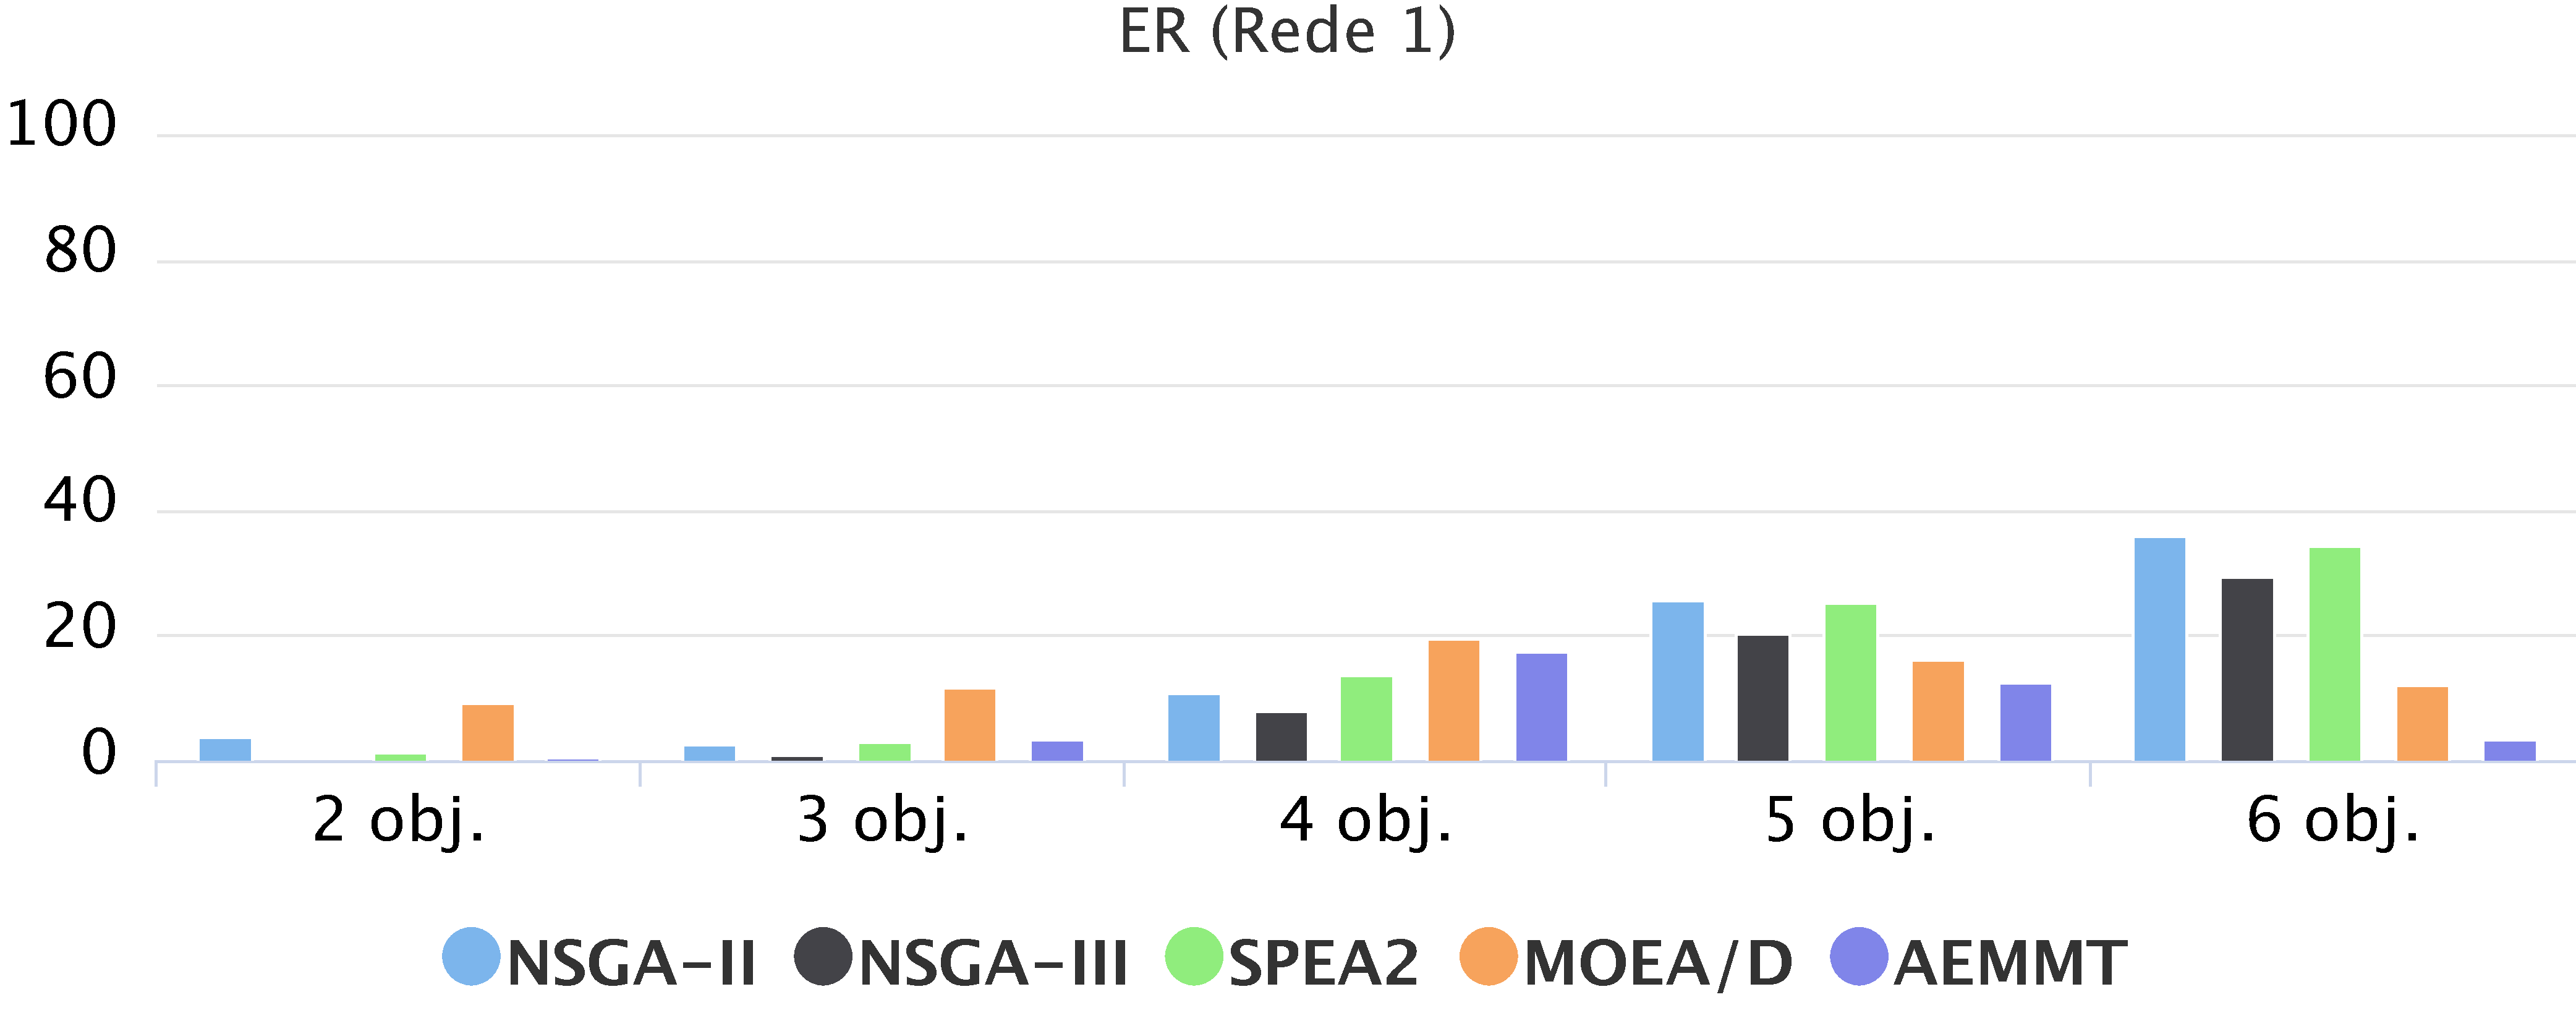
\includegraphics[width=1\textwidth]{cap_experimentos/figs/etapa1/er-mrp-r1}
	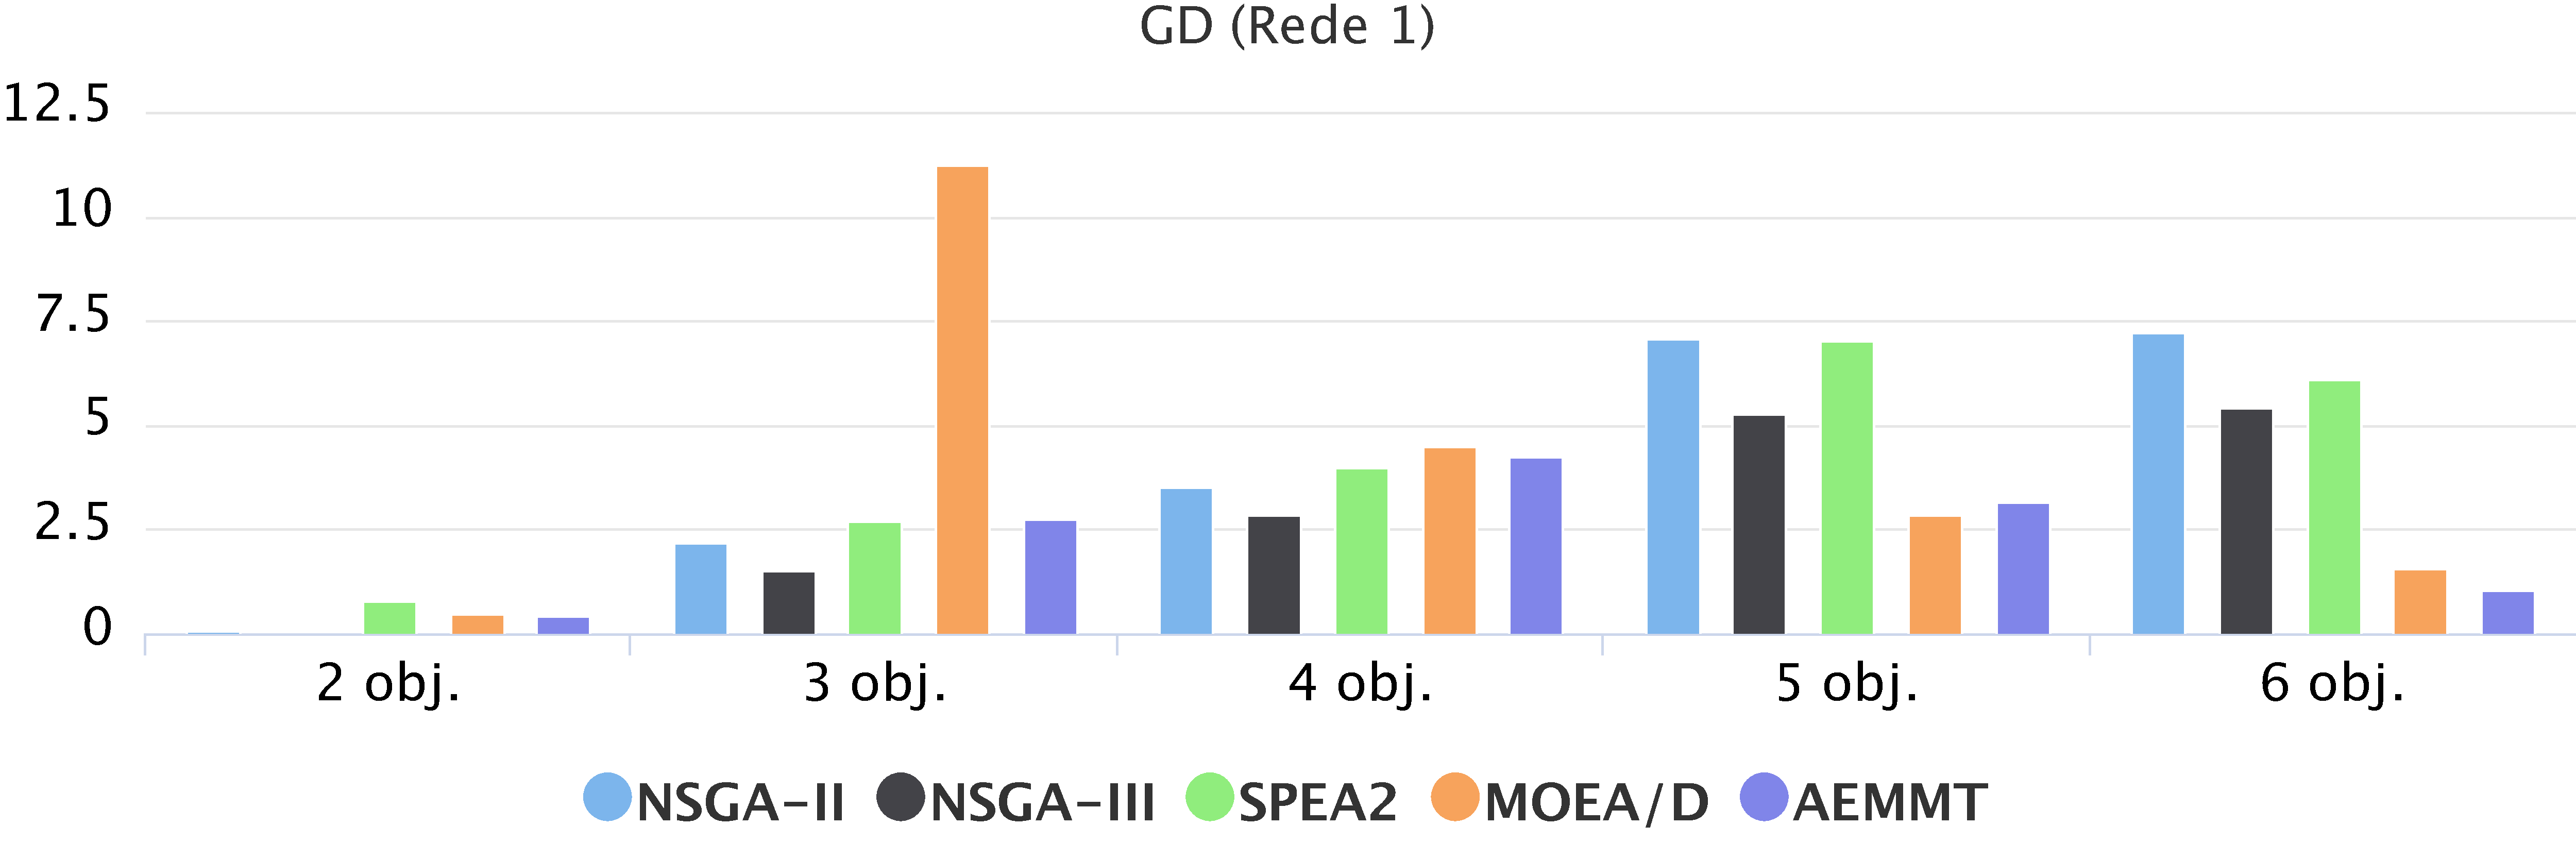
\includegraphics[width=1\textwidth]{cap_experimentos/figs/etapa1/gd-mrp-r1}
	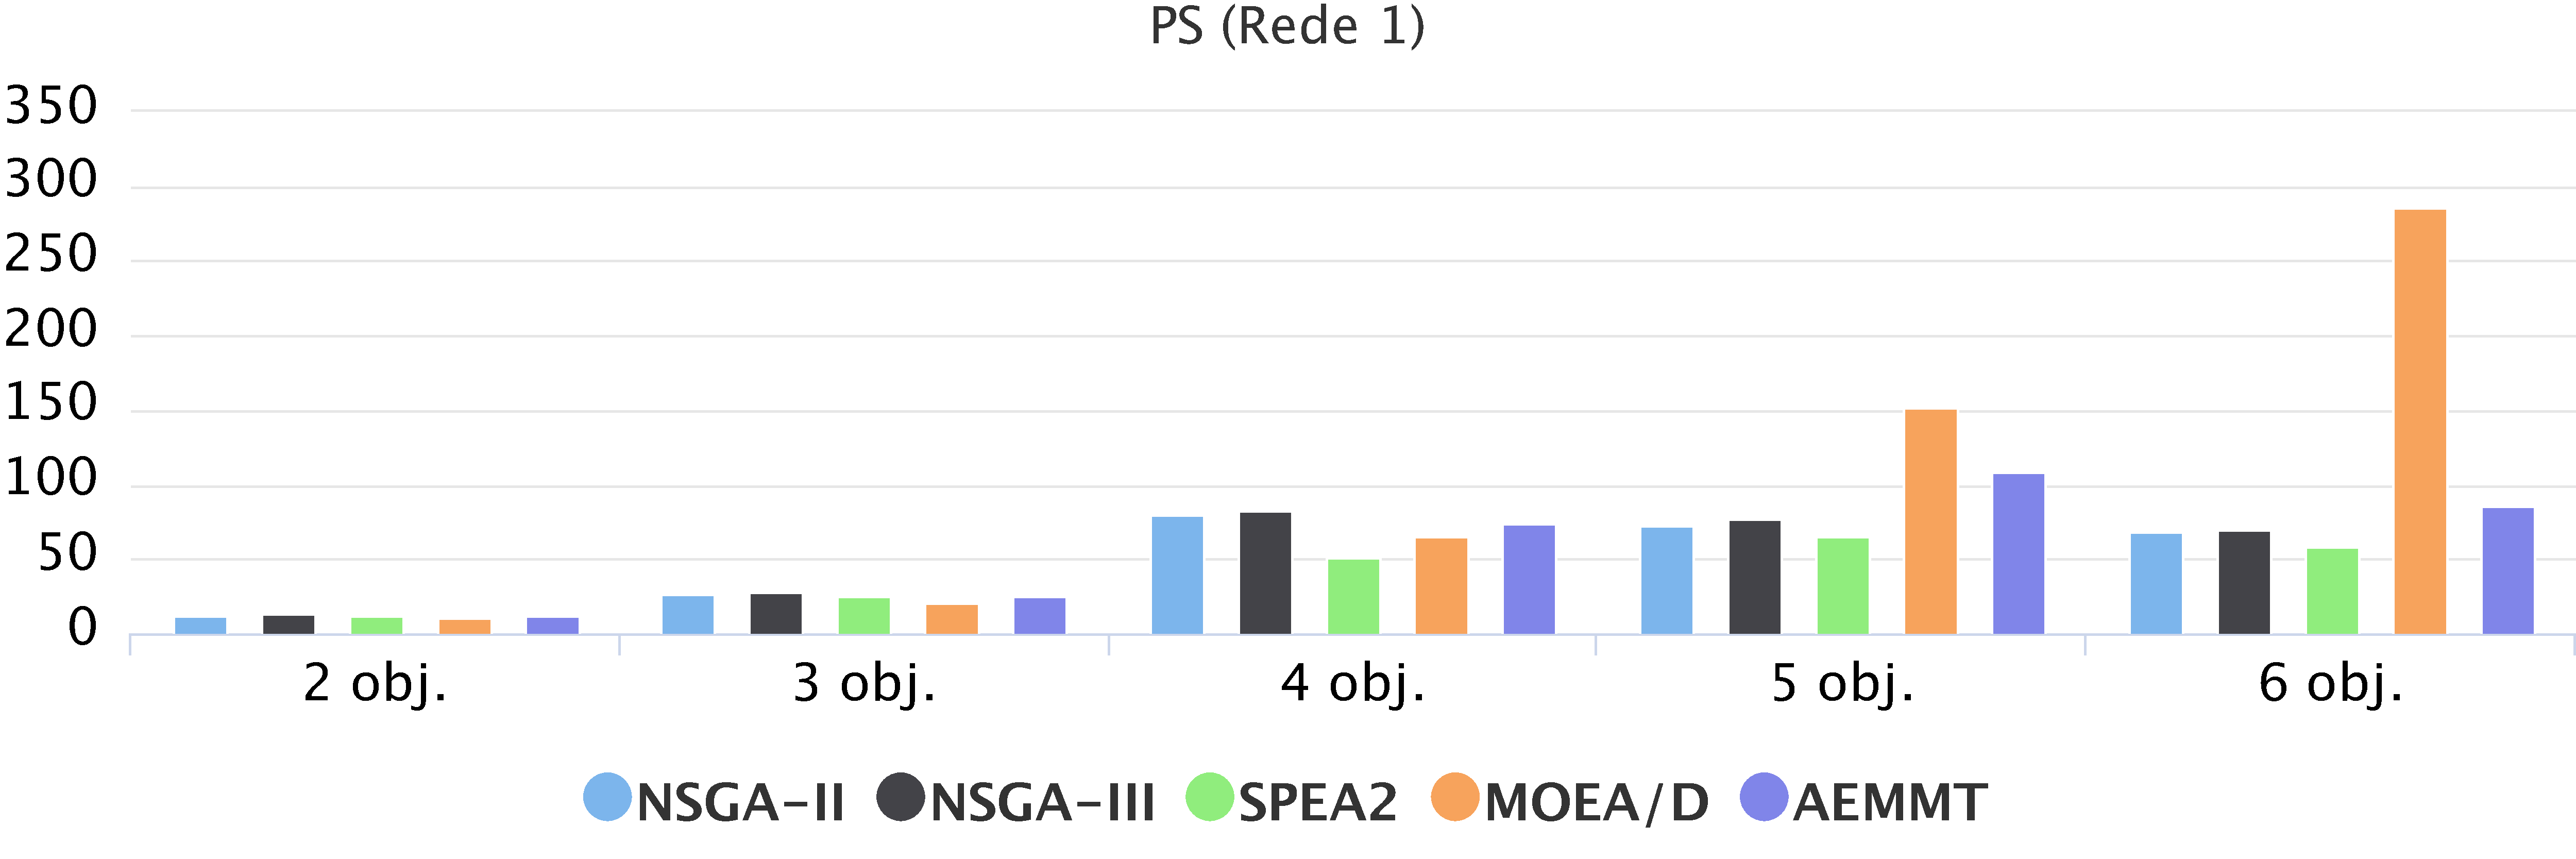
\includegraphics[width=1\textwidth]{cap_experimentos/figs/etapa1/ps-mrp-r1}
	\caption{\label{fig_exp1_prm_r1}Desempenho dos algoritmos na 1ª etapa para o PRM na rede 1}
\end{figure*}

Na \autoref{fig_exp1_prm_r1} são apresentados os desempenhos dos AEMOs na resolução do PRM para a rede 1. Essa é a instância mais simples testada e retornou baixas taxas de erro para todos os algoritmos. Considerando todas as formulações de objetivo, o maior valor de $ER$ foi obtido pelo NSGA-II aplicado ao problema de 6 objetivos (36,3\%). Diferentemente do esperado, o NSGA-III mostrou o melhor resultado ($ER$, $GD$ e $PS$) para os problemas com 2, 3 e 4 objetivos. A partir de 5 objetivos, o AEMMT e o MOEA/D são os dois melhores métodos, sendo que o primeiro apresenta uma menor taxa de erro, enquanto o segundo obtém uma fronteira de soluções não-dominadas de maior cardinalidade. Para poucos objetivos, o NSGA-III é claramente o melhor método, para 5 ou mais critérios de otimização, ambos AEMMT e MOEA/D são boas opções.

\begin{figure*}[!htbp]	
	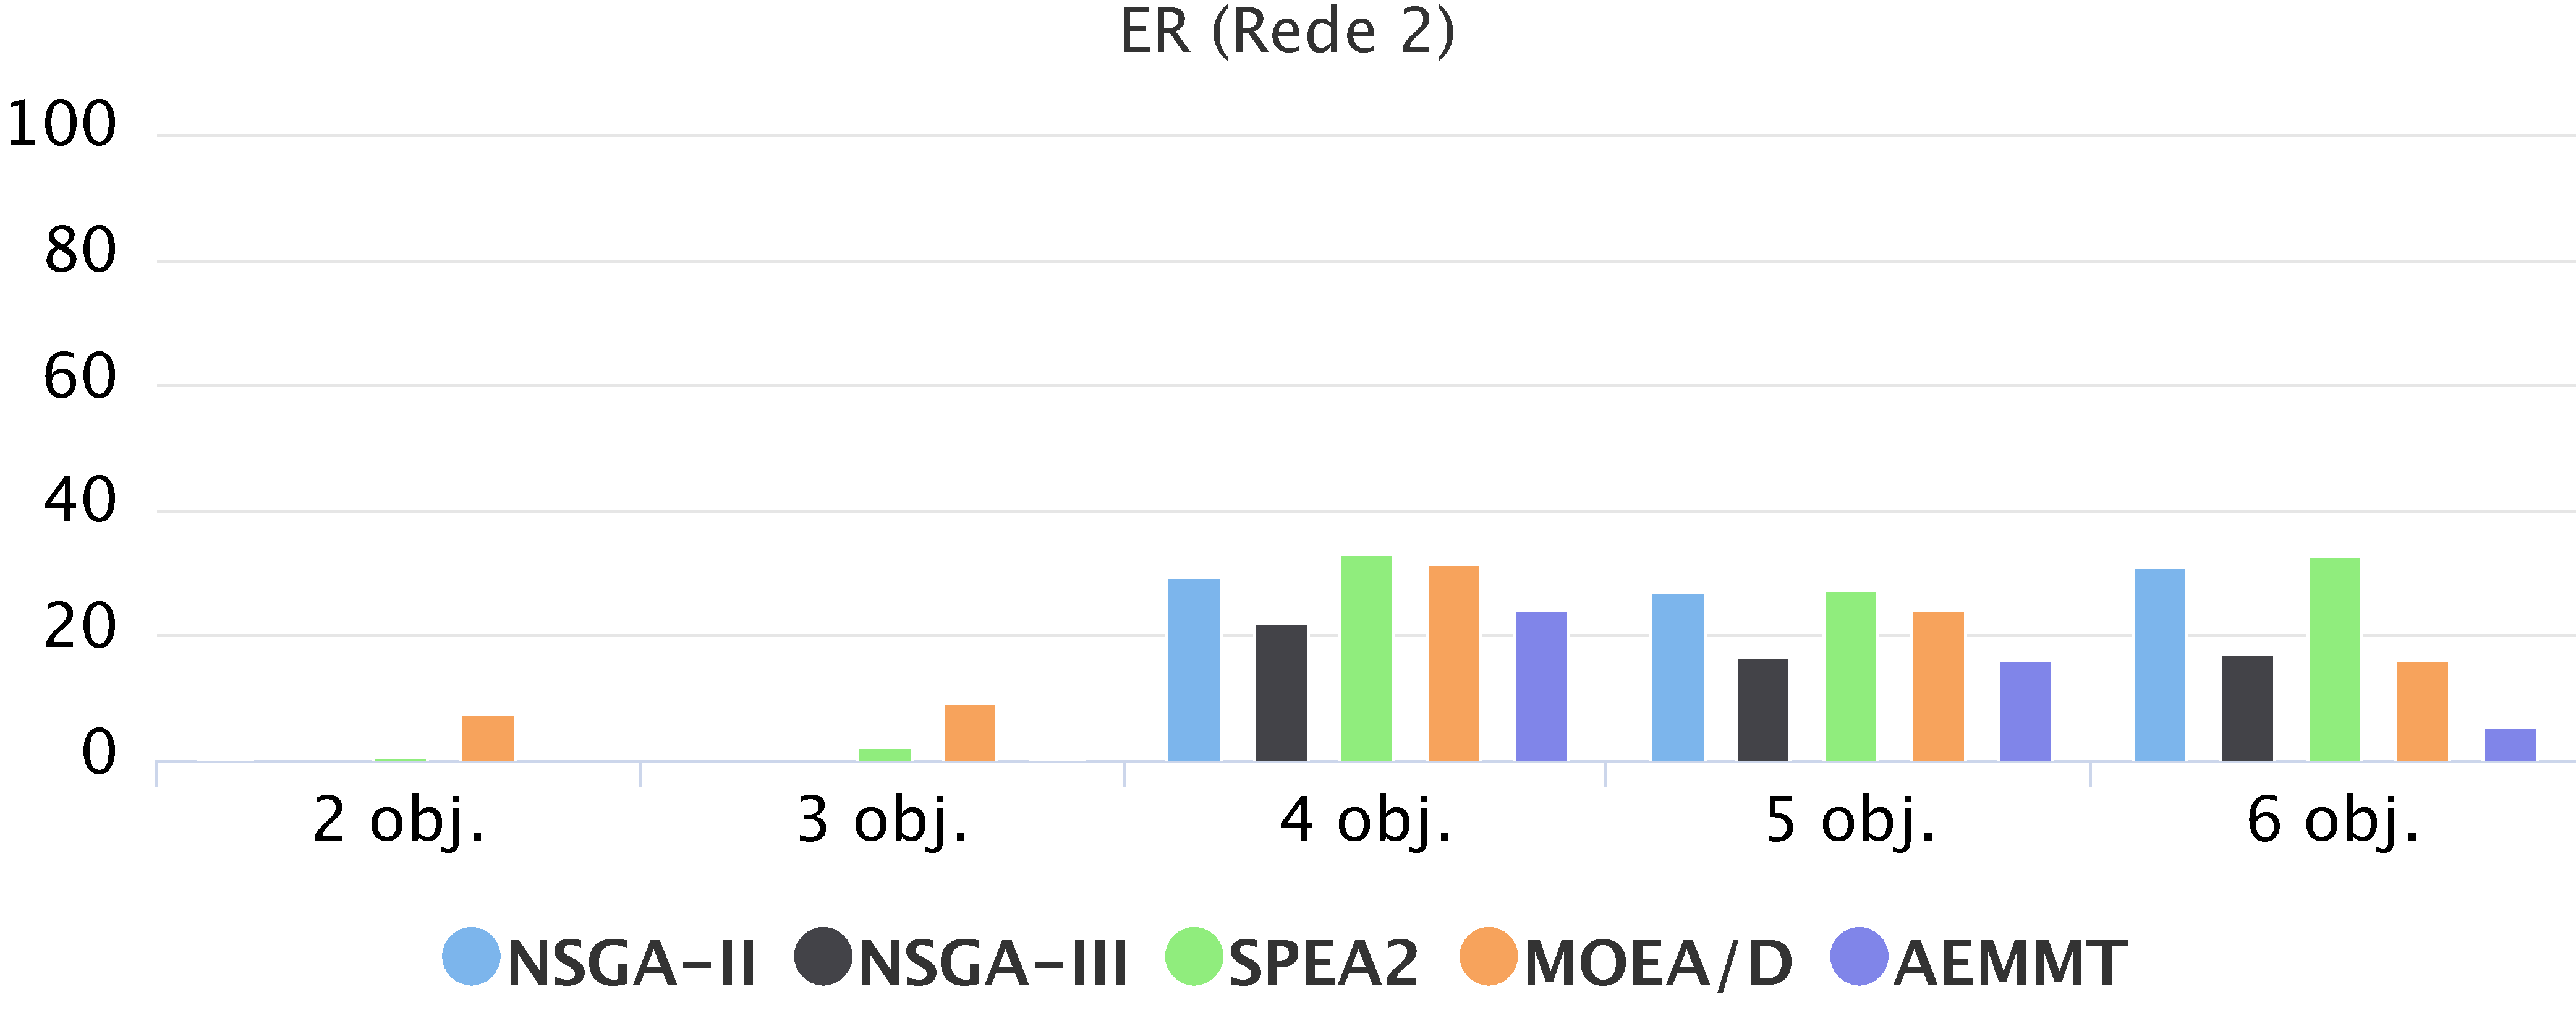
\includegraphics[width=1\textwidth]{cap_experimentos/figs/etapa1/er-mrp-r2}
	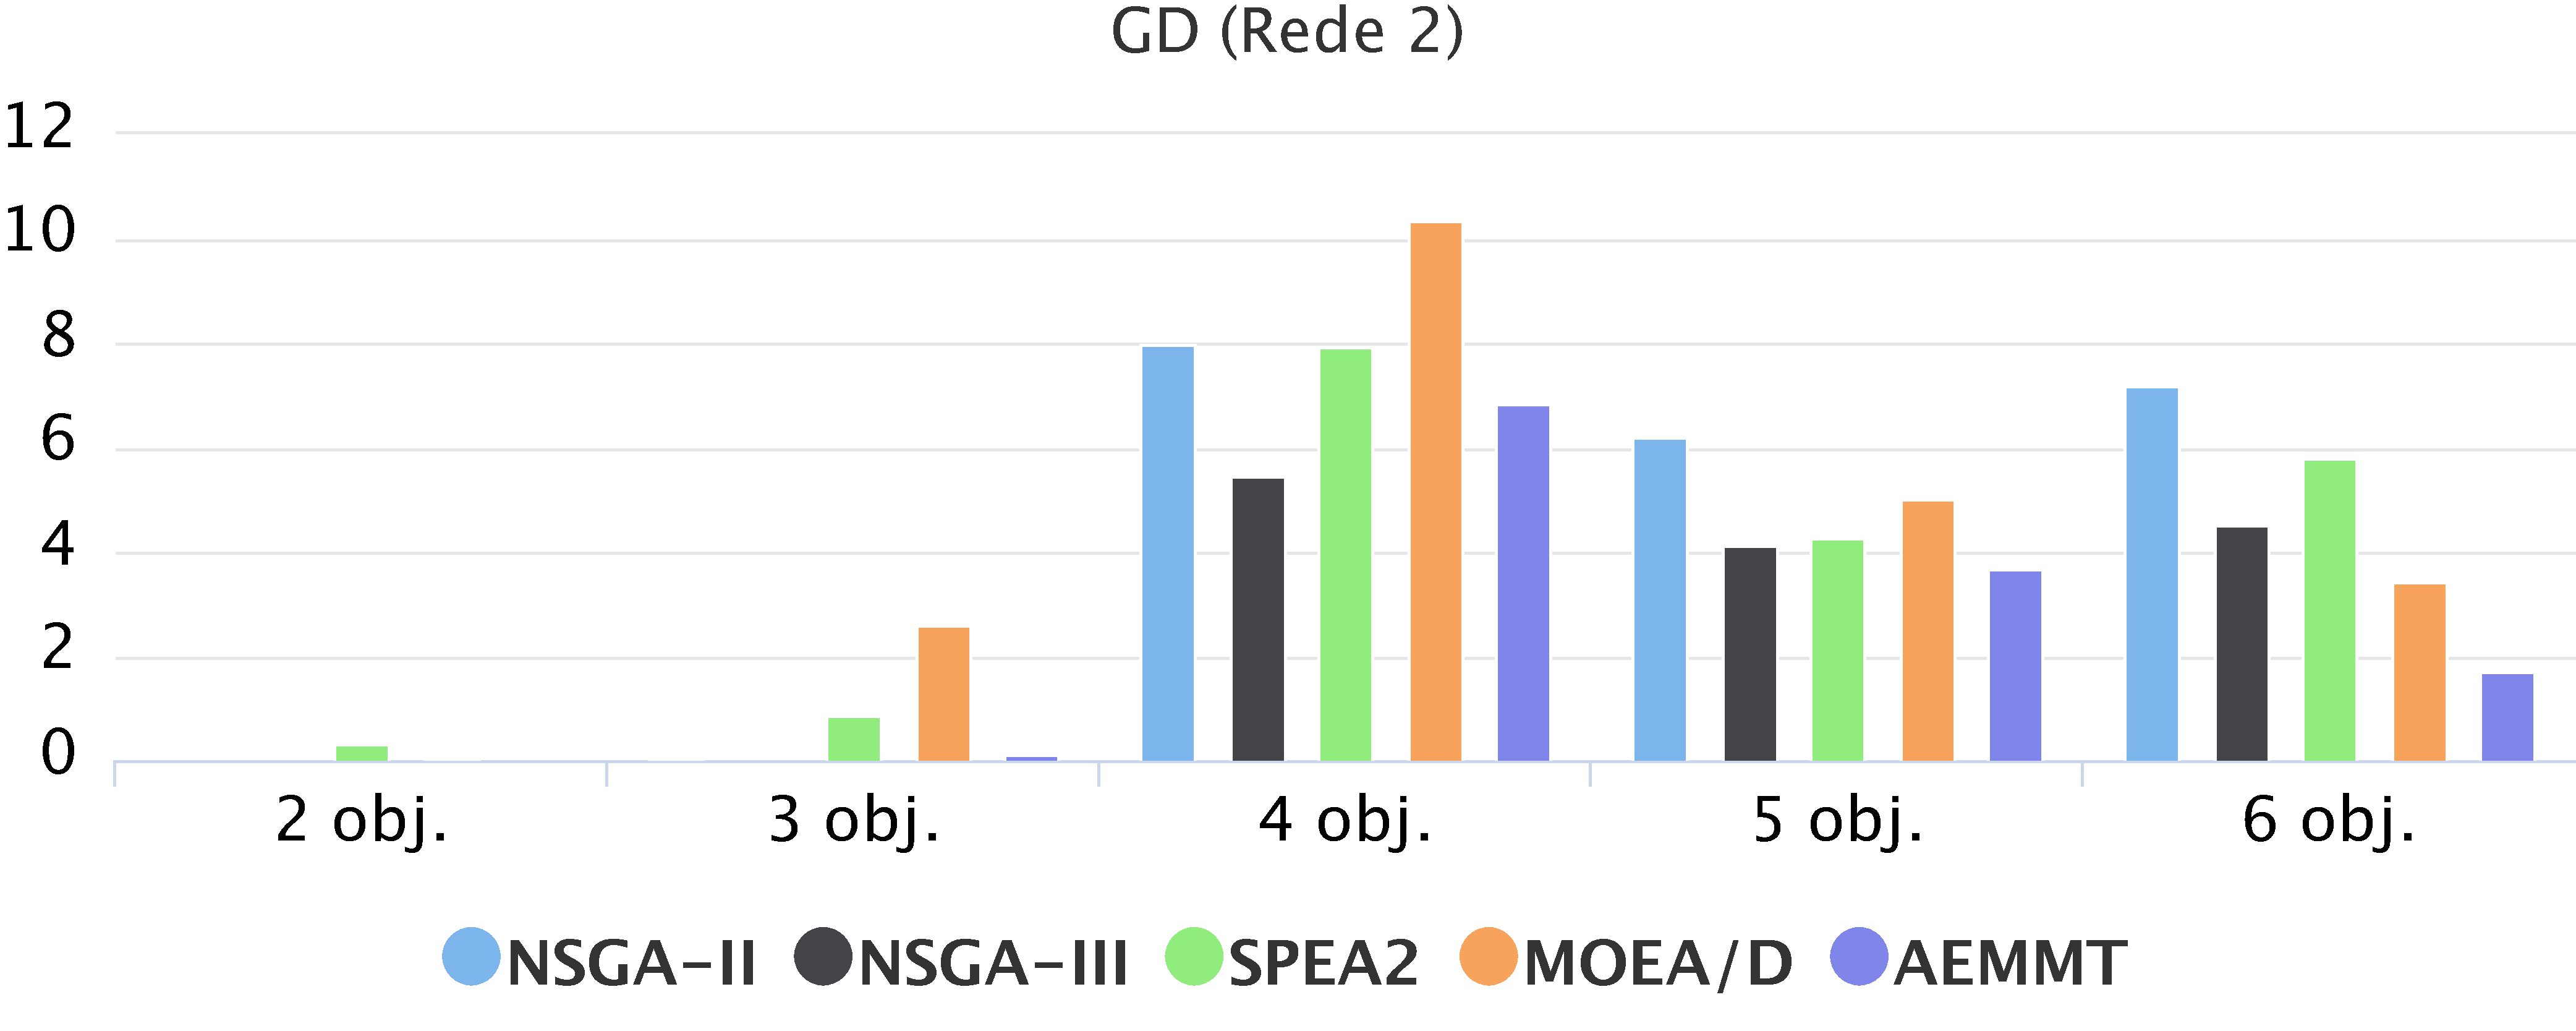
\includegraphics[width=1\textwidth]{cap_experimentos/figs/etapa1/gd-mrp-r2}
	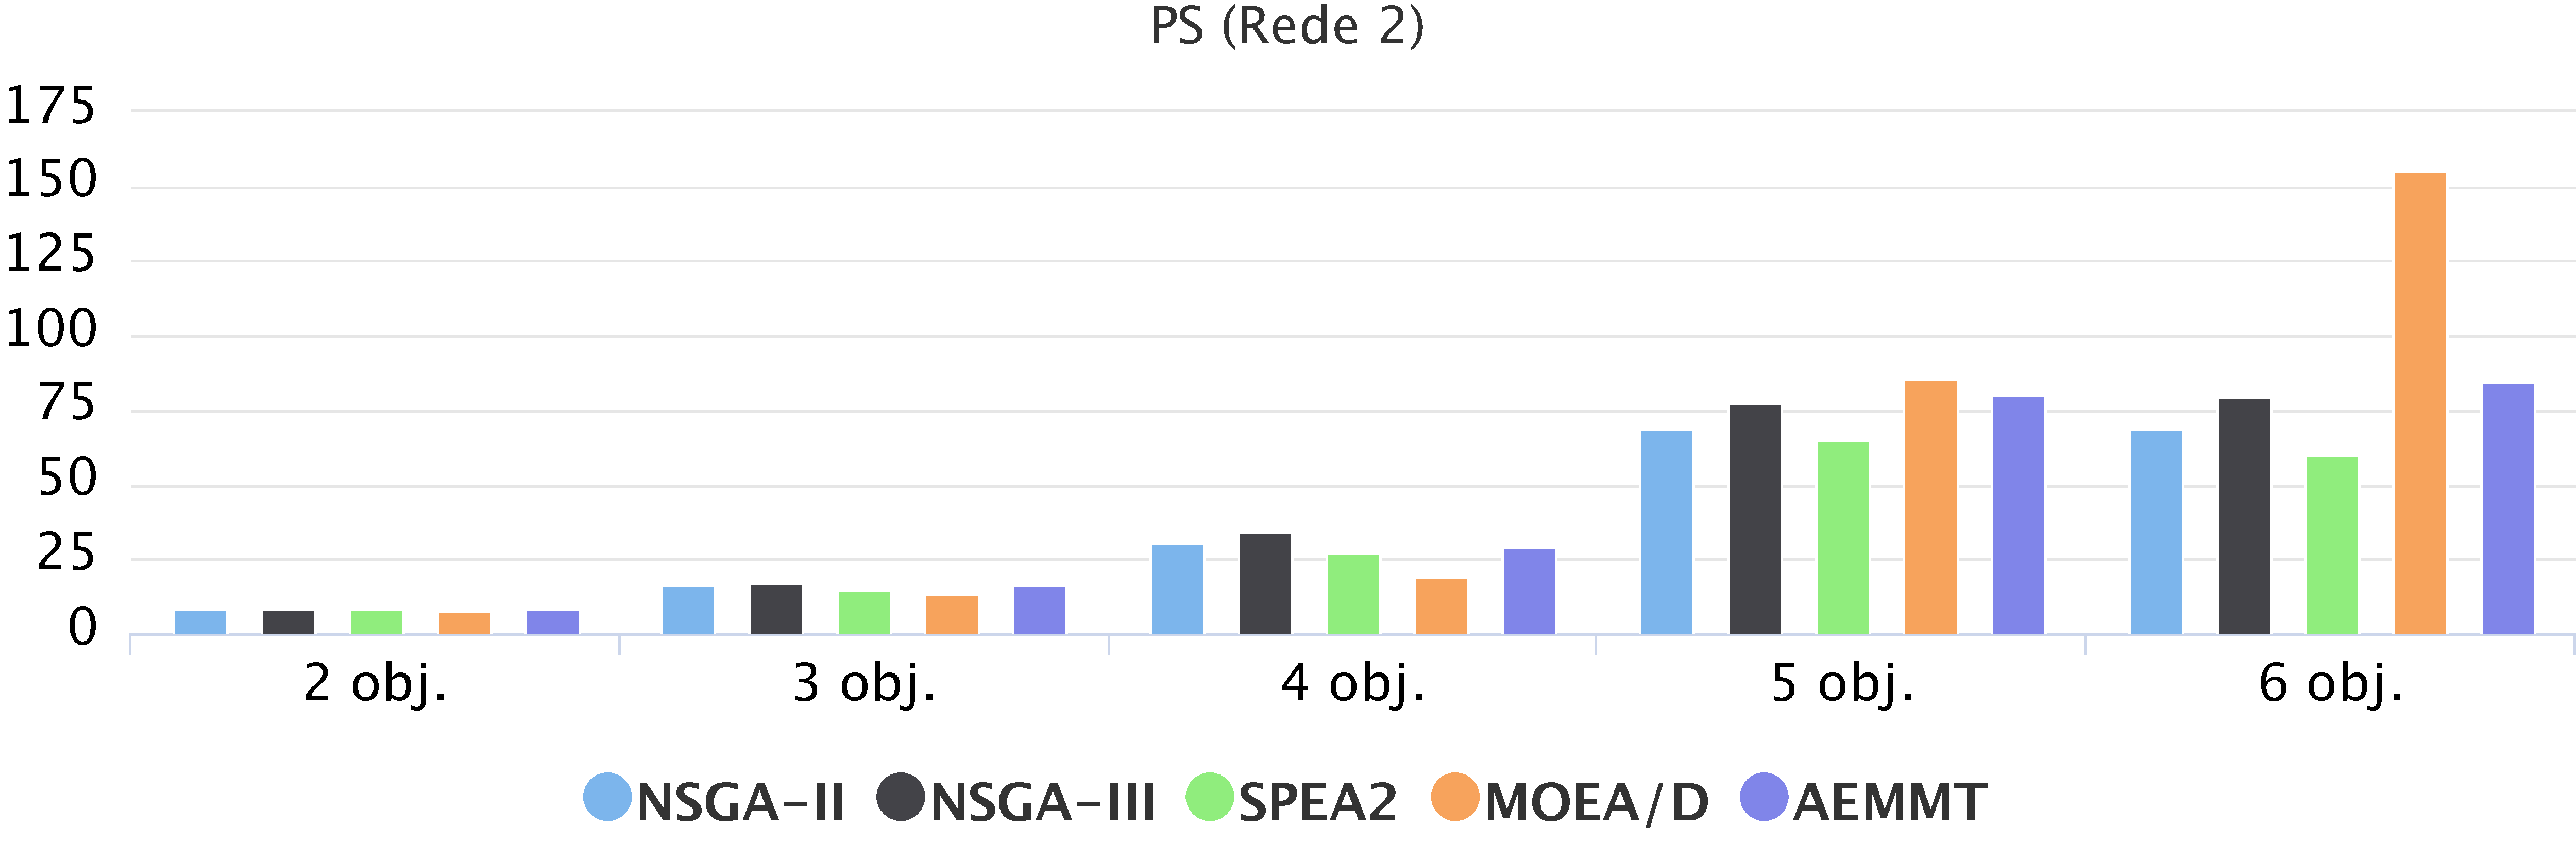
\includegraphics[width=1\textwidth]{cap_experimentos/figs/etapa1/ps-mrp-r2}
	\caption{\label{fig_exp1_prm_r2}Desempenho dos algoritmos na 1ª etapa para o PRM na rede 2}
\end{figure*}

Considerando o desempenho dos AEMOs para o PRM com a rede 2 (\autoref{fig_exp1_prm_r2}), o NSGA-III é o melhor algoritmo nos problemas com 2, 3 e 4 objetivos, em qualquer uma das métricas, seguido pelo NSGA-II e SPEA2. Para 5 objetivos, o AEMMT apresenta a menor taxa de erro (16,6\%), seguido de perto pelo NSGA-III (16,9\%). Com relação ao $GD$ no problema de 5 objetivos, o AEMMT obtém o melhor desempenho, mas o NSGA-III e o SPEA2 atingem valores similares. Em termos de $PS$, o MOEA/D, o AEMMT e o NSGA-III conseguem valores bem similares, sendo o MOEA/D o melhor dentre eles. Para 6 objetivos, os menores $ER$ e $GD$ foram obtidos pelo AEMMT (3,6\%; 1,7), em primeiro lugar, pelo MOEA/D (16,3\%; 3,4), em segundo e pelo NSGA-III (17,4\%; 4,5), em terceiro. Os melhores valores de $PS$ foram apresentados pelo MOEA/D (155,4), que ficou bem a frente dos segundo e terceiro melhores algoritmos (AEMMT com 84,8 e NSGA-III com 79,9). Nos cenários com poucos objetivos, o NSGA-III mostrou ser a melhor opção para a rede 2, enquanto nos com 5 ou mais objetivos, é preferível utilizar o AEMMT, caso uma baixa taxa de erro seja desejável, ou o MOEA/D, caso deseja-se um maior conjunto de soluções não-dominadas.

\begin{figure*}[!htbp]
	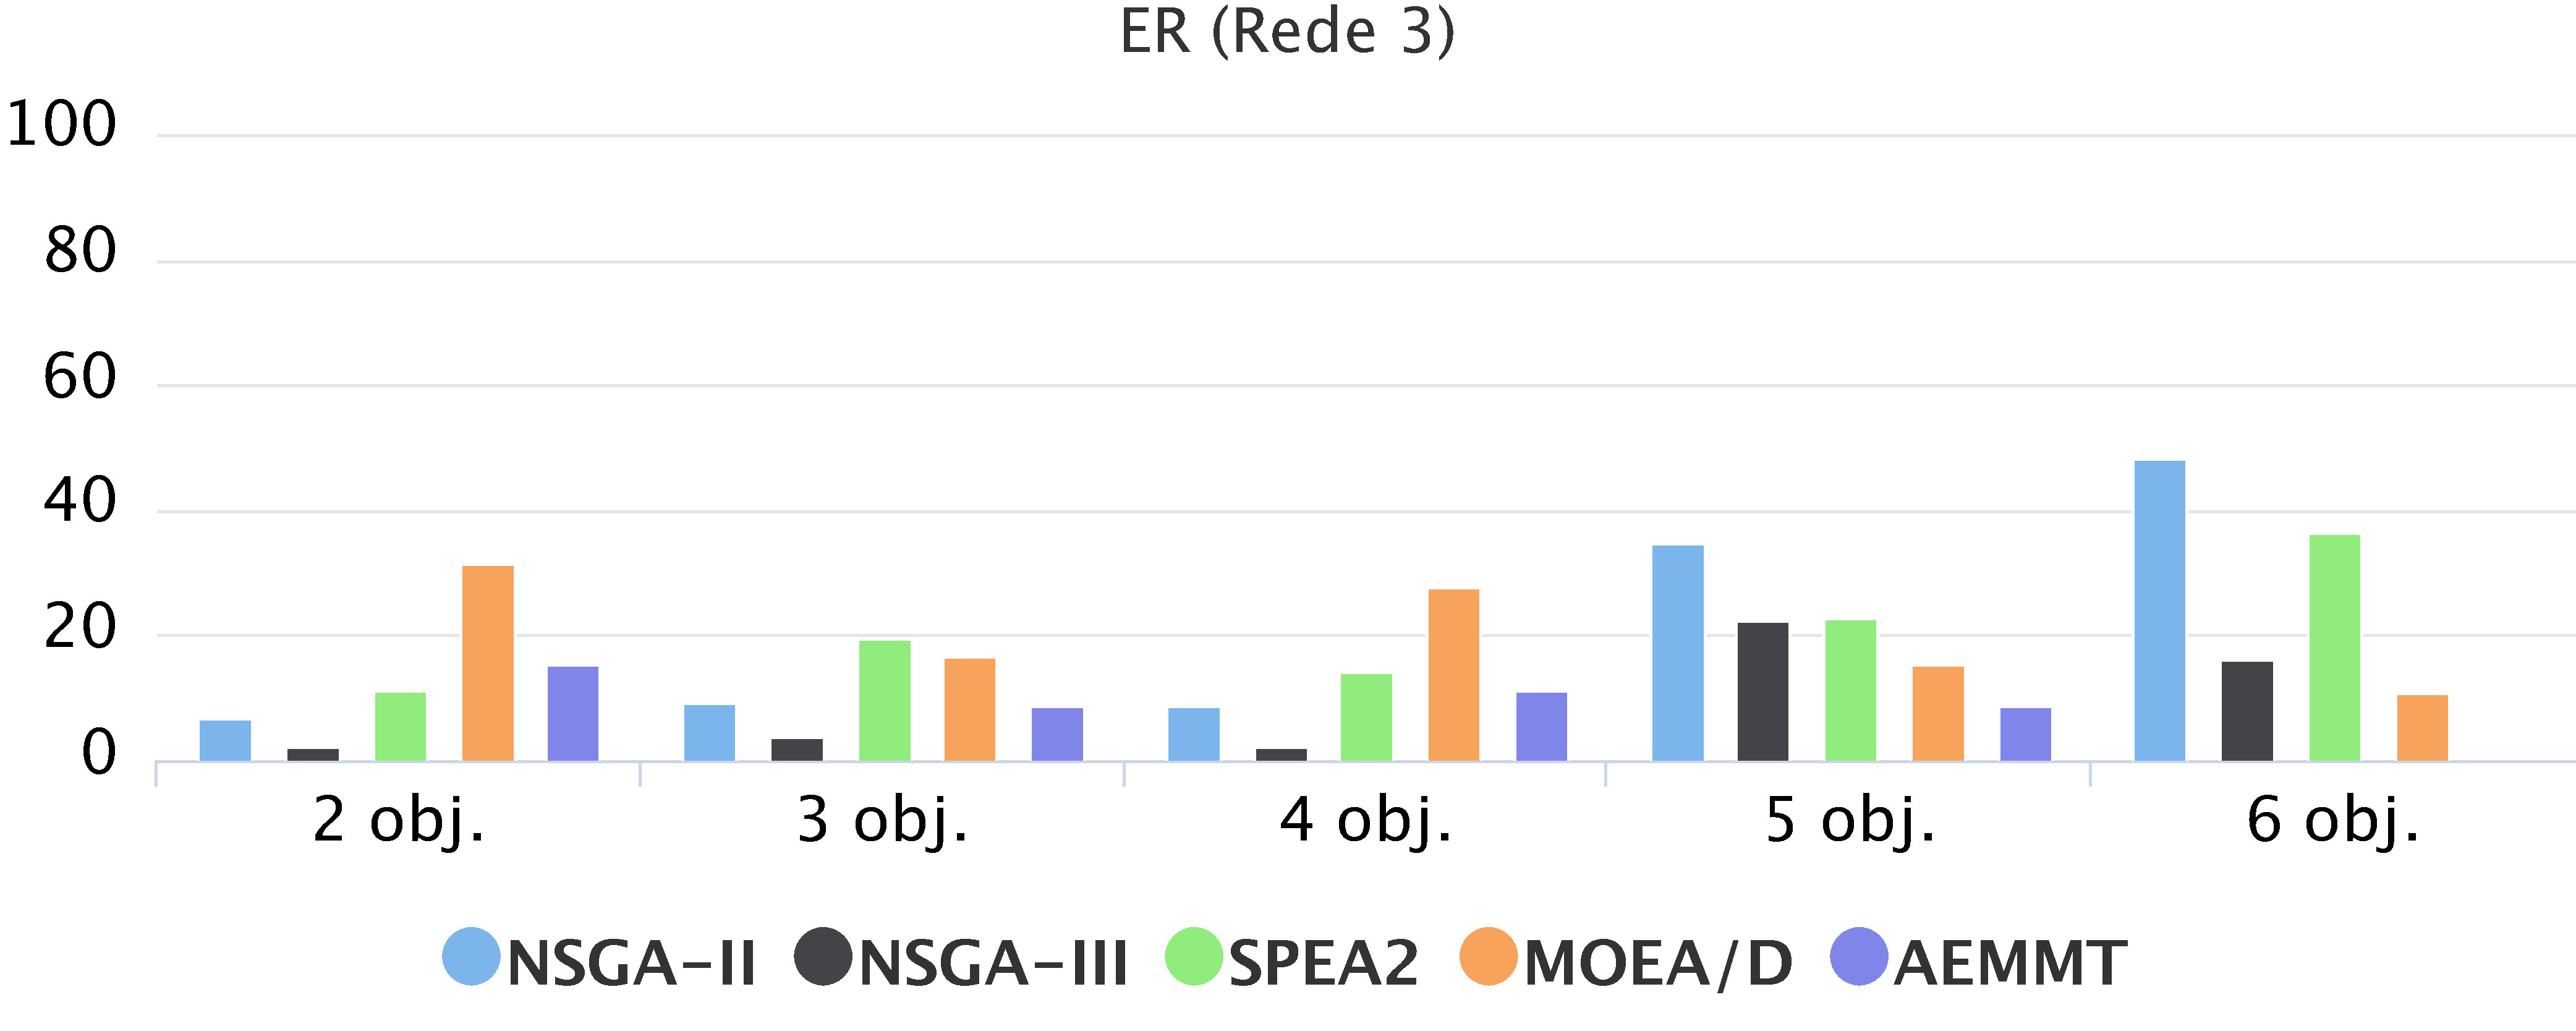
\includegraphics[width=1\textwidth]{cap_experimentos/figs/etapa1/er-mrp-r3}
	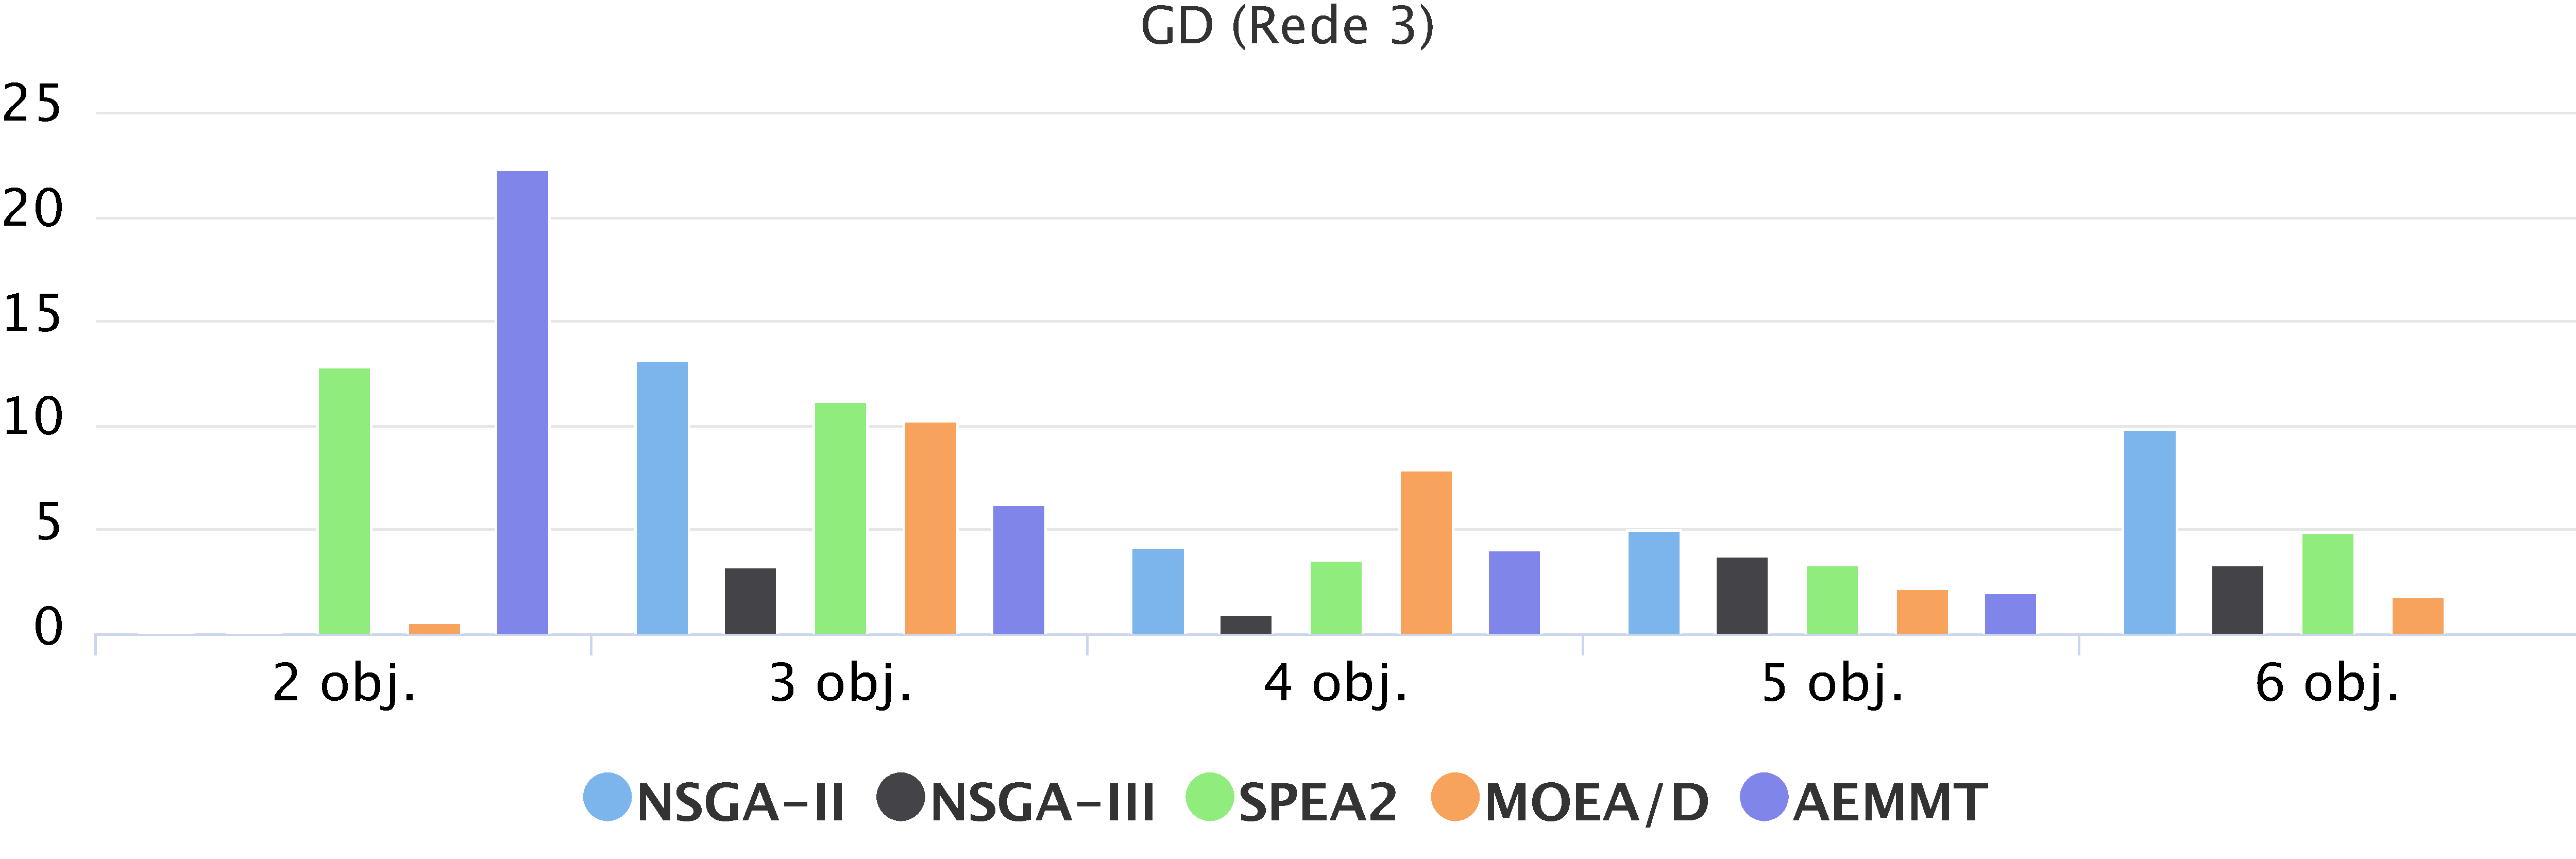
\includegraphics[width=1\textwidth]{cap_experimentos/figs/etapa1/gd-mrp-r3}
	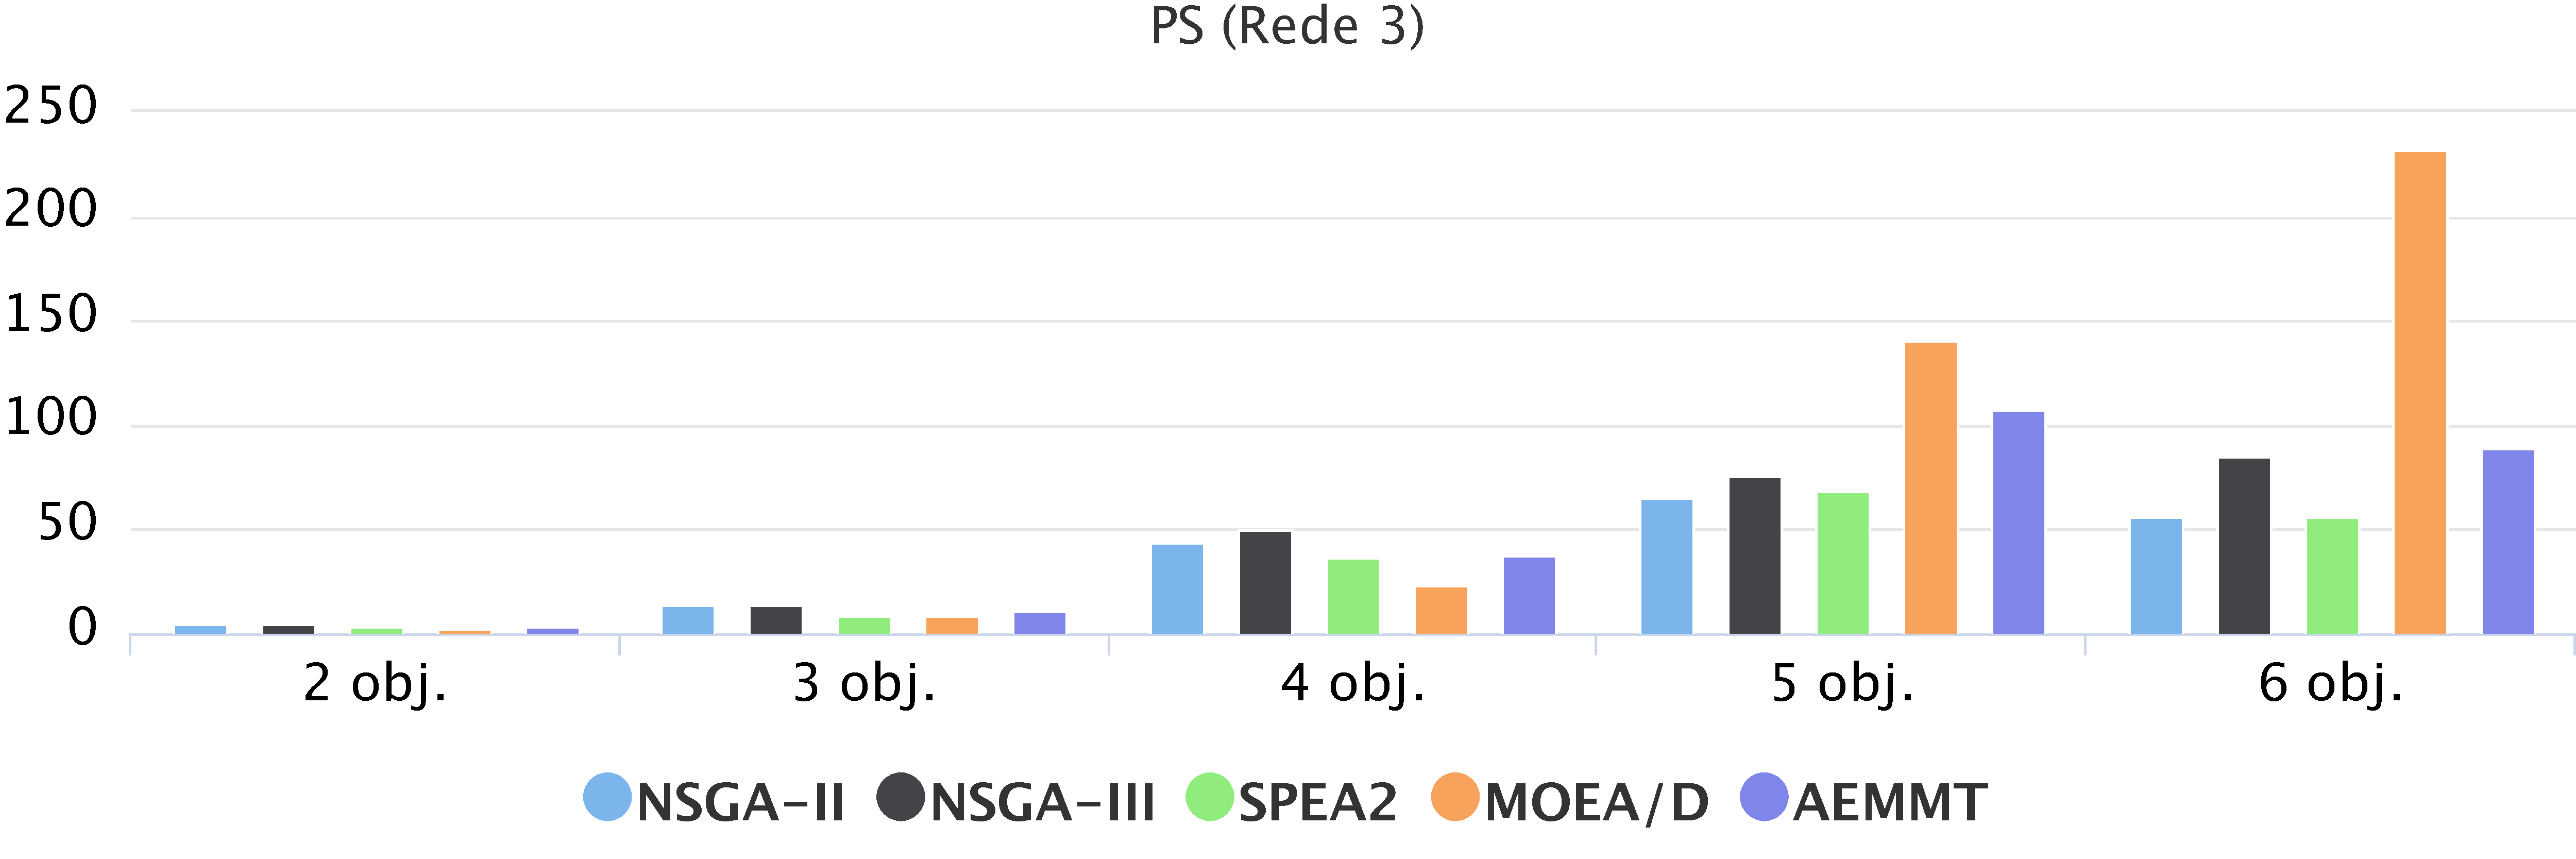
\includegraphics[width=1\textwidth]{cap_experimentos/figs/etapa1/ps-mrp-r3}
	\caption{\label{fig_exp1_prm_r3}Desempenho dos algoritmos na 1ª etapa para o PRM na rede 3}
\end{figure*}

A rede 3 é a mais complexa analisada nesta etapa dos experimentos. Analisando-se os resultados dos gráficos apresentados na \autoref{fig_exp1_prm_r3}, a tendência já observada nas demais instâncias é mantida, na qual o NSGA-III continua sendo o melhor método para as formulações com poucos objetivos. Até 4 objetivos, em todas as métricas, o NSGA-III apresenta os melhores resultados. Para 5 e 6 objetivos, o AEMMT apresenta menor $ER$ e $GD$, enquanto o MOEA/D consegue maior $PS$.

\begin{figure*}[!htbp]	
	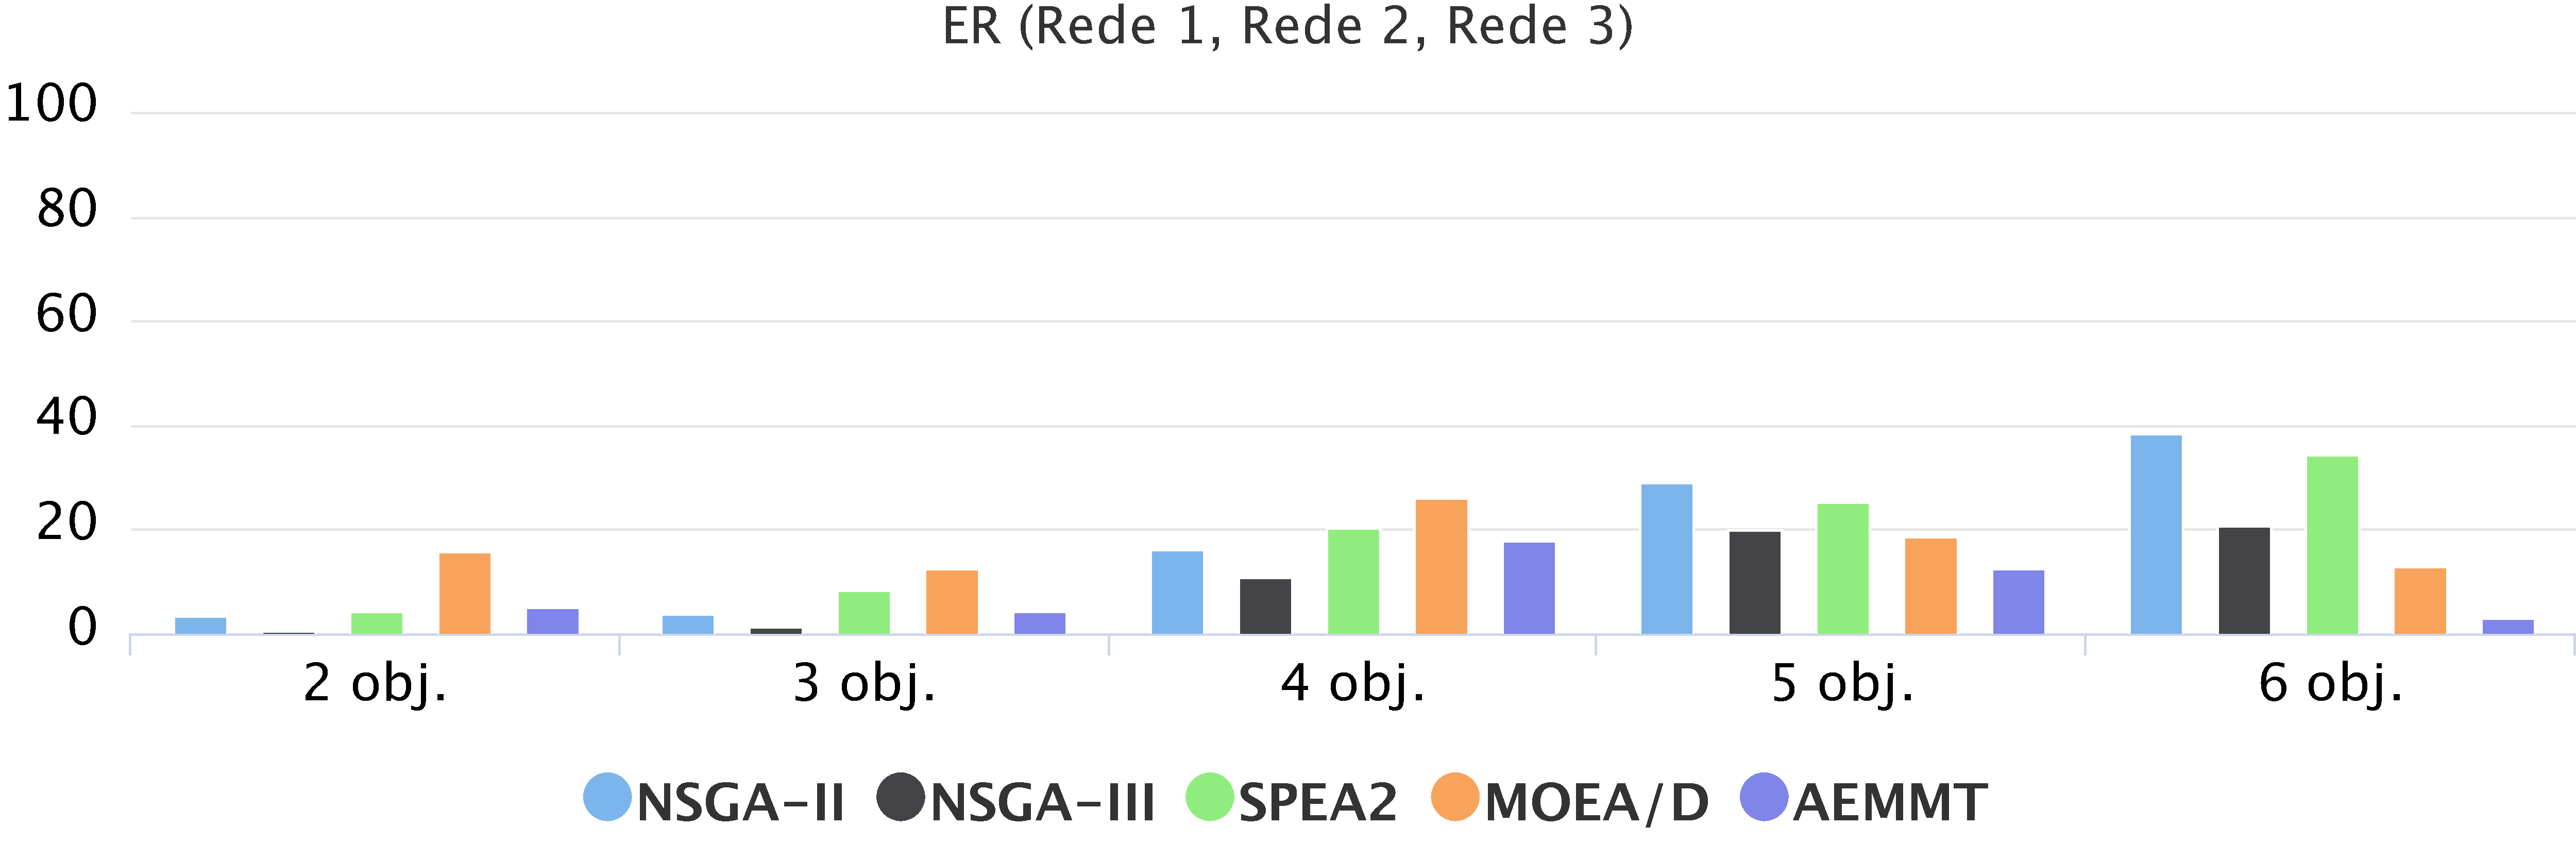
\includegraphics[width=1\textwidth]{cap_experimentos/figs/etapa1/er-mrp-todos}
	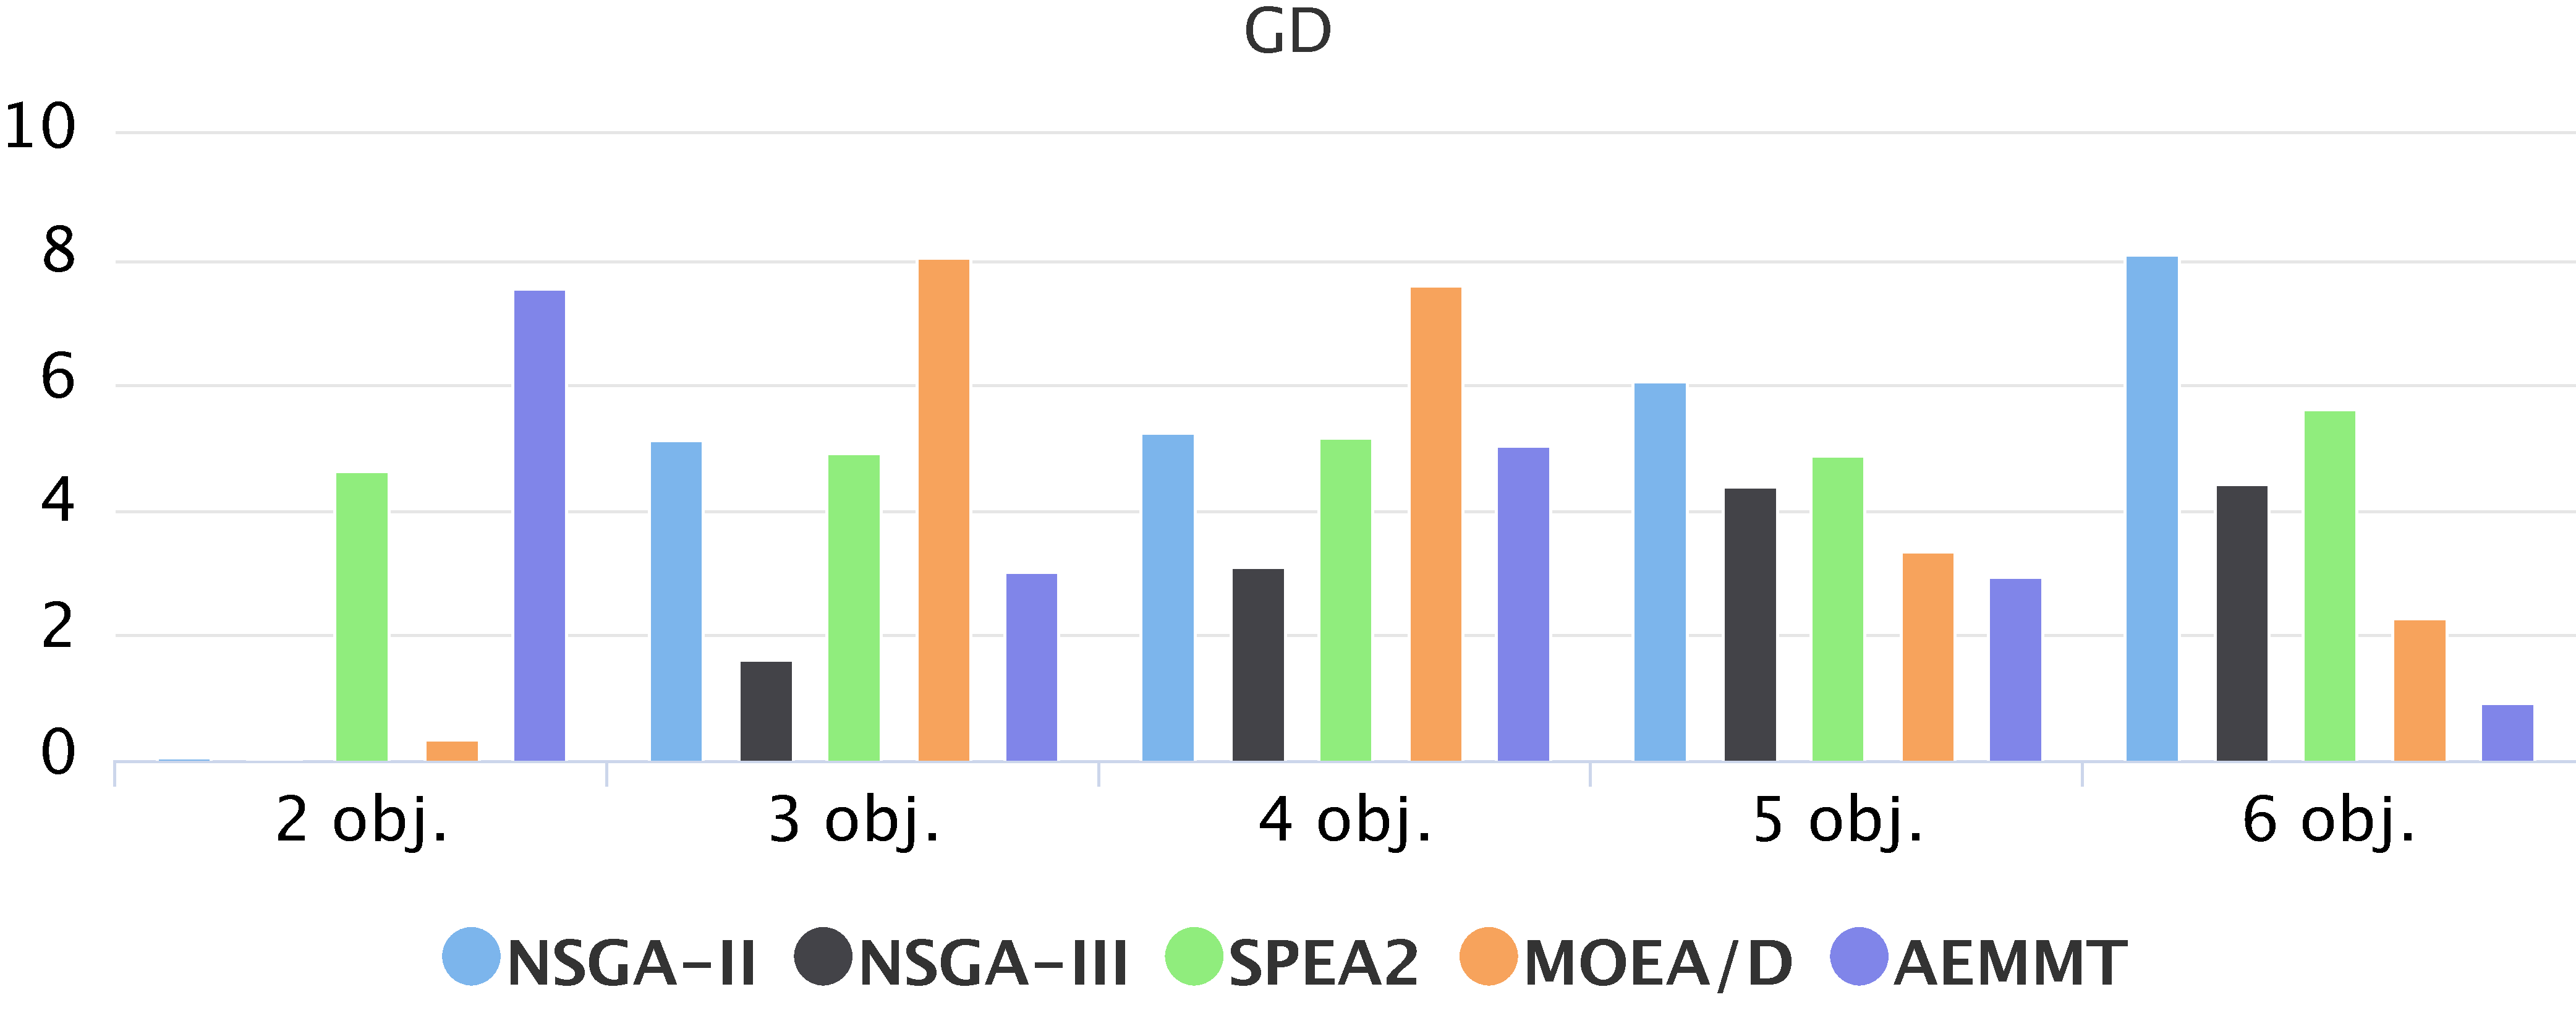
\includegraphics[width=1\textwidth]{cap_experimentos/figs/etapa1/gd-mrp-todos}
	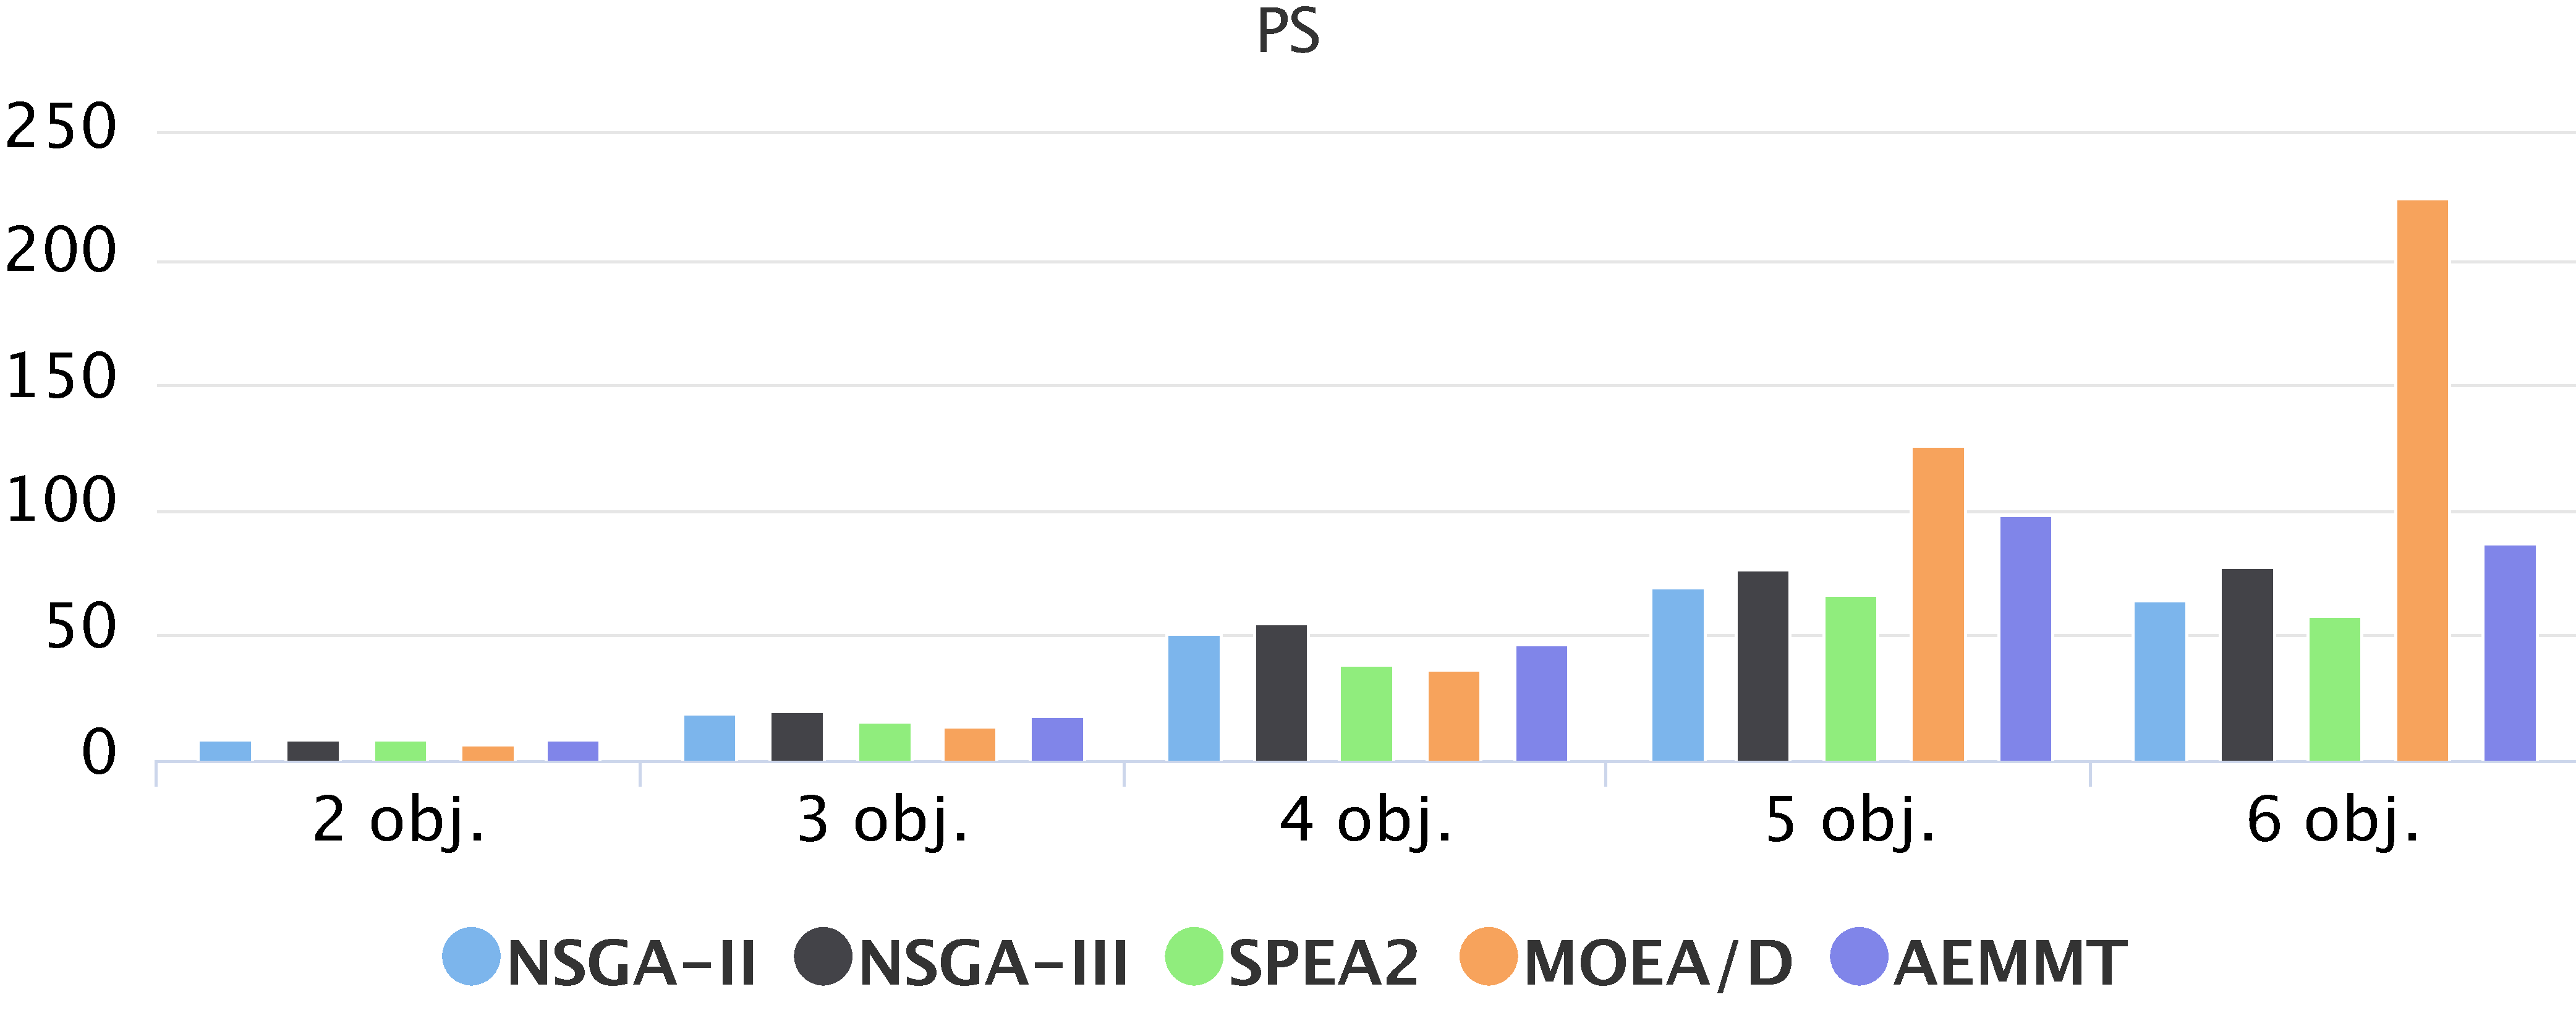
\includegraphics[width=1\textwidth]{cap_experimentos/figs/etapa1/ps-mrp-todos}
	\caption{\label{fig_exp1_prm_todos}Resultado consolidado da 1ª etapa considerando o PRM nas redes 1, 2, e 3}
\end{figure*}

A fim de fazer uma análise geral do PRM, os desempenhos dos algoritmos em todas as instâncias do problema (redes 1, 2 e 3) são consolidados nos gráficos da \autoref{fig_exp1_prm_todos}. Assim como no PMM, essa consolidação é obtida através da média aritmética dos valores das métricas em cada instância. Apesar de ser esperado que o NSGA-II e o SPEA2 fossem os melhores métodos para poucos objetivos, a partir dos gráficos da \autoref{fig_exp1_prm_todos}, observa-se que o NSGA-III obteve o melhor resultado para as formulações com 2, 3 e 4 objetivos. O NSGA-II também atinge bons resultados para 2 e 3 objetivos, mas o SPEA2 apresenta um $GD$ relativamente ruim. Considerando problemas de 5 e 6 objetivos, a escolha do algoritmo depende do intuito da busca. Se a quantidade encontrada de soluções do Pareto for mais relevante, o MOEA/D é mais indicado. Por outro lado, se um menor erro é preferível, então o AEMMT é a melhor opção.

Considerando-se ambos os problemas, PMM e PRM, os algoritmos NSGA-II, SPEA2 e NSGA-III são os que geram melhores resultados para problemas com poucos objetivos. O desempenho dos algoritmos clássicos (NSGA-II e SPEA2) diminui consideravelmente à medida que se aumenta o número de objetivos. Em contrapartida, o desempenho dos métodos AEMMT e MOEA/D melhora a partir de quatro objetivos, tornando-os mais indicados para problemas \textit{many-objectives}.

Outra observação que pôde ser feita a partir dos experimentos desta etapa é que o AEMMT perde apenas em $PS$ para o MOEA/D. Uma das características do AEMMT é a limitação no tamanho do arquivo, o que levanta a seguinte questão: se não houvesse esse limite, o AEMMT alcançaria melhor resultado em todas as métricas? Visando responder tal questão, foram executados novos experimentos para avaliar o desempenho de uma variação do AEMMT (AEMMT-F), na qual não existe um limite para o tamanho do arquivo. Na maioria dos experimentos, o AEMMT-F apresentou uma taxa de erro maior que sua versão original. Em contrapartida, essa variação alcançou valores médios para as métricas $ER$ e $PS$ melhores que aqueles obtidos pelo MOEA/D, principalmente para as formulações com 5 e 6 objetivos (\textit{many-objective}). Essa superioridade foi confirmada através de um teste de hipótese paramétrico, chamado de teste Z (\textit{Z-test}) com 0,1\% de significância ($\alpha = 0,1$) \cite{Franca2018}. Os novos resultados obtidos pelo AEMMT-F permitem dizer que ele é preferível em relação ao MOEA/D, mas não é necessariamente melhor que o algoritmo AEMMT original, que continua sendo a melhor opção em termos de taxa de erro ($ER$). 

Considerando que essa dissertação visa estratégias para lidar com problemas com muitos objetivos, para as próximas etapas serão utilizados apenas cenários a partir de 4 objetivos. Da mesma forma, os AEMOs tradicionais (NSGA-II e SPEA2) não serão mais avaliados e os experimentos serão realizados apenas com os algoritmos \textit{many-objective}.

\section{Etapa 2: Análise das estratégias e configurações para o MACO/NDS}
\label{section_experimentos_etapa2}

Na elaboração do novo algoritmo ACO para a manipulação de problemas \textit{many-objective}, fez-se necessário um estudo sobre os métodos para a construção das soluções pelas formigas no PRM. Além disso, foi também preciso testar modelos de atualização de feromônio e ideias sobre os parâmetros de entrada $\alpha$ e $\beta$ do algoritmo. A fim de propor o novo método de otimização \textit{many-objective} e um modelo de aplicação para o PRM, realizou-se a segunda etapa de experimentos, onde várias configurações possíveis do algoritmo e do modelo foram testadas.

Inicialmente, um modelo de construção das soluções do PRM para colônia de formigas foi concebido de acordo com os experimentos realizados nesta etapa. O mesmo processo não foi realizado para o PMM, pois o modelo descrito em \cite{Alaya2004} para algoritmos ACO se mostrou adequado desde os primeiros experimentos com o novo modelo \textit{many-objective}. Além disso, nesses experimentos também avaliaram-se diferentes aspectos sobre a atualização de feromônios e parâmetros de entrada no ACO, resultando em particularidades do algoritmo proposto.

Os experimentos dessa etapa foram realizados em duas fases. A primeira investiga o impacto de diferentes modelos de construção das soluções no desempenho do algoritmo proposto. Nesses experimentos, optou-se por simplificar o problema investigado a partir da adoção de um cenário com um único objetivo (mono-objetivo), possibilitando a avaliação, de maneira isolada, do processo de construção das soluções. Os experimentos da segunda fase visam analisar a influência de mudanças nas estratégias e configurações adotadas pelo MACO/NDS para resolver problemas multiobjetivos. Essas mudanças envolvem a construção de soluções por amostragem, formas de depósito de feromônio e dinamização dos parâmetros de entrada. Os experimentos de cada fase são descritos a seguir.

Nos experimentos com o problema mono-objetivo, foram avaliadas quatro estratégias (descritas na Seção \ref{section_algoritmo_prm}):

\begin{enumerate}
	\item Formiga única: o espaço de busca é explorado de forma aleatória, mas sempre considerando apenas a vizinhança da posição atual da formiga.
	\item Múltiplas formigas: uma formiga para cada destino. Unem-se os caminhos produzidos por cada agente em uma árvore.
	\item Formiga com sobreposição quântica: uma formiga explora o espaço de busca de forma aleatória, podendo estar em vários nós ao mesmo tempo. Essa estratégia elimina o problema de localidade na busca.
	\item Formigas invertidas: uma formiga para cada destino, mas ao invés construírem uma trajetória da raiz ao destino, fazem o caminho contrário, ou seja, partem do destino e tentam encontrar a raiz.
\end{enumerate}

O problema mono-objetivo utilizado consiste em minimizar o valor do produto entre custo e atraso ($f(x) = custo(x) \times delay(x)$) de uma árvore. Portanto, quanto menor esse valor, melhor a árvore obtida. Além das quatro estratégias avaliadas, também foi implementada uma modificação do algoritmo de Prim \cite{Prim1957} para servir como referência de uma solução potencial para o PRM. Cada estratégia foi executada cinco vezes e a tabela \ref{tab_exp2_estrategias} mostra o resultado da melhor execução de cada estratégia. Nessa tabela, a coluna ``resultado'' representa a soma dos valores de $custo \times delay$ das arestas da árvore obtida como solução. Ou seja, quanto menor esse valor, melhor a solução obtida.

\begin{table}[!htbp]
	\centering
	\caption{Desempenho em função da estratégia de construção de uma solução para o PRM}
	\label{tab_exp2_estrategias}
	\begin{tabular}{rrrr}
		Estratégia & Rede & Resultado   & Tempo (s)    \\ \hline
		Prim       & $R_1$   & 3,28 & 0,02     \\
		1          & $R_1$   & 3,04 & 2,49     \\
		2          & $R_1$   & 3,03 & 5,94      \\
		\rowcolor{table-green} 
		3          & $R_1$   & 3,00 & 3,88      \\
		\rowcolor{table-green} 
		4          & $R_1$   & 3,00 & 3,16      \\ \hline
		Prim       & $R_2$   & 3,13 & 0,01     \\
		1          & $R_2$   & 3,34 & 4,94     \\
		2          & $R_2$   & 3,26 & 13,22     \\
		\rowcolor{table-green} 
		3          & $R_2$   & 3,13 & 10,69    \\
		4          & $R_2$   & 3,30 & 5,549     \\ \hline
		Prim       & $R_3$   & 7,96 & 0,024     \\
		1          & $R_3$   & 8,13 & 4,212     \\
		2          & $R_3$   & 8,23 & 25,60    \\
		\rowcolor{table-green} 
		3          & $R_3$   & 7,48 & 9,82     \\
		4          & $R_3$   & 8,11 & 6,93     \\ \hline
		Prim       & $R_4$   & 1,80 & 0,02     \\
		1          & $R_4$   & 2,34 & 4,71     \\
		2          & $R_4$   & 2,32 & 12,47    \\
		\rowcolor{table-green} 
		3          & $R_4$   & 1,85 & 11,01    \\
		4          & $R_4$   & 1,97 & 4,93     \\ \hline
		Prim       & $R_5$   & 6,34 & 0,01     \\
		1          & $R_5$   & 6,12 & 6,87      \\
		2          & $R_5$   & 6,33 & 17,38     \\
		\rowcolor{table-green} 
		3          & $R_5$   & 5,85 & 14,76    \\
		\rowcolor{table-green} 
		4          & $R_5$   & 5,85 & 8,42     \\ \hline
	\end{tabular}
\end{table}

Como pode ser observado na tabela, a estratégia número 3, que usa a ideia de formiga com sobreposição, obteve o melhor valor para a função objetivo (resultado). Os valores obtidos por essa estratégia foram inclusive melhores que os obtidos pelo algoritmos utilizado como referência (Prim). Em contrapartida, ela foi a segunda pior estratégia em relação ao tempo. Por essa razão, propõe-se a ideia de amostragem explicada na Seção \ref{section_algoritmo_prm}. Ao invés de se utilizar todo o conjunto de exploração, a construção da solução é realizada sobre uma amostra dele. Em nossos experimentos para o PRM, a amostragem é de 10 elementos. A Tabela \ref{tab_exp2_amostragem} mostra uma comparação dos melhores valores obtidos utilizando a estratégia 3, com e sem essa amostragem.

\begin{table}[!htbp]
	\centering
	\caption{Resultados obtidos a partir da estratégia 3 de acordo com o espaço de exploração considerado (com e sem amostragem)}
	\label{tab_exp2_amostragem}
	\begin{tabular}{rrrr}
		Amostragem    & Rede & Resultado   & Tempo (s) \\ \hline
		s/ amostragem & $R_1$    & 3 & 3,88      \\
		\rowcolor{table-green}
		c/ amostragem & $R_1$    & 3 & 3,41      \\ \hline
		s/ amostragem & $R_2$    & 3,13 & 10,69    \\
		\rowcolor{table-green}
		c/ amostragem & $R_2$    & 3,13 & 7,60     \\ \hline
		s/ amostragem & $R_3$    & 7,48 & 9,82     \\
		\rowcolor{table-green}
		c/ amostragem & $R_3$    & 7,48 & 7,26      \\ \hline
		s/ amostragem & $R_4$    & 1,85 & 11,01    \\
		\rowcolor{table-green}
		c/ amostragem & $R_4$    & 1,78 & 7,28      \\ \hline
		s/ amostragem & $R_5$    & 5,85 & 14,76    \\
		\rowcolor{table-green}
		c/ amostragem & $R_5$    & 5,76  & 10,03    \\ \hline
	\end{tabular}
\end{table}

Como pode ser observado na Tabela \ref{tab_exp2_amostragem}, a amostragem não só diminuiu o tempo do algoritmo como também melhorou o resultado para as redes mais complexas ($R_5$ e $R_6$). O aumento da qualidade da solução pode ser atribuído ao maior grau de aleatoriedade dado ao algoritmo, similar ao que acontece nos algoritmos genéticos quando se lança mão de operações como a mutação ou seleções por torneio.

A partir desses resultados, implementou-se a primeira versão do novo algoritmo ACO \textit{many-objective}, que chamamos aqui de MACO/NDS-alpha. O MACO/NDS-alpha conta com a estratégia 3 (formiga com sobreposição quântica) e amostragem do espaço de exploração. Ao aplicarmos essa primeira versão do algoritmo no PRM \textit{many-objetive}, percebeu-se que o AEMMD atingiu um desempenho muito superior ao do novo algoritmo, como apresentado na Tabela \ref{tab_exp2_macod_simples}. Nessa etapa, o AEMMD foi adotado como referência, uma vez que, até onde se sabe, é o algoritmo que teve o melhor desempenho no PRM \textit{many-objective} \cite{LafetaThesis}. Tal observação nos motivou a buscar novas melhorias no modelo a ser proposto. Assim, depois de alguns testes preliminares, duas modificações foram incorporadas ao modelo baseado em ACO:

\begin{itemize}
	\item Depósito de feromônio baseado na qualidade da aresta (ou do item, no caso do PMM): em um problema multiobjetivo, ao depositar feromônios sobre as arestas correspondentes às soluções não-dominadas, normalmente é utilizada a mesma quantidade independentemente da solução e da aresta. Isso ocorre porque, segundo a relação de não-dominância, ambas opções são igualmente boas. Entretanto, nossa nova estratégia muda esse conceito, relacionando a quantidade de feromônios depositada à qualidade da aresta. Nesse contexto, considerando que é um problema de minimização, a quantidade passa a ser inversamente proporcional à soma dos pesos da aresta.
	\item Dinamização do parâmetro de entrada $\beta$: esse parâmetro controla a importância da heurística no cálculo das probabilidades de cada aresta (ou item, no PMM) fazer parte da solução. Nossa proposta é diminuir um pouco a importância da heurística, dando maior peso à informação de feromônio sempre que, após uma iteração, não for encontrada uma nova solução. Esse processo se repete a cada iteração até que uma nova solução é encontrada, o valor de $\beta$ é reiniciado para o padrão (fornecido como entrada para o algoritmo).
\end{itemize}

O algoritmo resultante foi chamado de \textit{Many-objective Ant Colony Optimization based on Non-dominated Decomposed Sets} (MACO/NDS). Considerando a formulação do PRM com seis objetivos, a Tabela \ref{tab_exp2_macod_simples} mostra as diferenças entre os desempenhos dos algoritmos AEMMD, MACO/NDS antes das alterações no depósito de feromônios e do parâmetro $\beta$ (MACO/NDS-alpha) e do algoritmo final proposto no capítulo \ref{chapter_macod} (MACO/NDS). A comparação é feita com base nos valores médios das métricas de desempenho multiobjetivo ($ER$, $GDp$ e $PS$).

\begin{table}[!htbp]
	\centering
	\caption{Análise comparativa entre as implementações do MACO/NDS e o AEMMD no PRM multiobjetivo (6 objetivos)}
	\label{tab_exp2_macod_simples}
	\begin{tabular}{rrrrr}
		Algoritmo  & Rede  & $ER$  & $GDp$ & $PS$  \\ \hline
		AEMMD      & $R_1$ & 6,59  & 0,38 & 502,8 \\
		MACO/NDS-alpha & $R_1$ & 18,42 & 0,30 & 337,6 \\
		MACO/NDS     & $R_1$ & 11,57 & 0,36 & 424,2 \\ \hline
		AEMMD      & $R_2$ & 7,58  & 0,49 & 296,6 \\
		MACO/NDS-alpha & $R_2$ & 11,75 & 0,47 & 284,4 \\
		MACO/NDS     & $R_2$ & 11,18 & 0,37 & 300   \\ \hline
		AEMMD      & $R_3$ & 11,73 & 0,19 & 388,6 \\
		MACO/NDS-alpha & $R_3$ & 36,47 & 0,16 & 206   \\
		MACO/NDS     & $R_3$ & 30,20 & 0,25 & 232,4 \\ \hline
		AEMMD      & $R_4$ & 35,88 & 0,17 & 234   \\
		MACO/NDS-alpha & $R_4$ & 54,48 & 0,11 & 150,2 \\
		MACO/NDS     & $R_4$ & 50,57 & 0,15 & 186,6 \\ \hline
		AEMMD      & $R_5$ & 32,67 & 0,20 & 181,2 \\
		MACO/NDS-alpha & $R_5$ & 32,95 & 0,22 & 168,6 \\
		MACO/NDS     & $R_5$ & 32,67 & 0,30 & 160,8
	\end{tabular}
\end{table}

Na Tabela \ref{tab_exp2_macod_simples}, pode-se observar que, na maioria dos casos, as duas alterações propostas melhoraram o resultado do MACO/NDS nas métricas ER e PS (nas quais o AEMMD é superior). Portanto, o algoritmo final proposto inclui essas duas alterações. Apesar do AEMMD ainda apresentar melhores resultados de desempenho, a nova versão do algoritmo conseguiu reduzir a diferença nas métricas $ER$ e $PS$.

Uma vez que foram definidas as estratégias e configurações que melhoram a qualidade dos resultados obtidos pelo método proposto, as próximas etapas visam analisar o desempenho do MACO/NDS em comparação com outros algoritmos many-objective bio-inspirados.

\section{Etapa 3: Análise comparativa entre o MACO/NDS e os AEMOs \textit{many-objective}}
\label{section_experimentos_etapa3}

Na terceira etapa, os experimentos visam avaliar a eficiência dos métodos de otimização \textit{many-objective} NSGA-III, MOEA/D, AEMMT, AEMMD e do algoritmo proposto, MACO/NDS, nos problemas da mochila e do roteamento multicast. Nessa etapa, foram utilizadas formulações com 4, 5 e 6 objetivos, avaliando-se 3 redes no PRM e problemas com 30, 40 e 50 itens no PMM. Os resultados dos experimentos revelam as vantagens e fraquezas do algoritmo proposto neste trabalho, possibilitando a identificação dos cenários nos quais sua utilização é mais adequada e as formas de melhorá-lo em cenários onde os seus resultados foram desfavoráveis. Esses experimentos representam a primeira vez em que o algoritmo AEMMD foi implementado para o PMM e também a primeira vez que o algoritmo proposto (MACO/NDS) foi implementado para o PMM e o PRM.

Por abordar apenas problemas com muitos objetivos (\textit{many-objective}), nesses experimentos foram descartados os AEMOs clássicos (NSGA-II e SPEA2) e incluídos os algoritmos AEMMD e o MACO/NDS (algoritmo proposto neste trabalho). Em todas as execuções, os algoritmos utilizaram os mesmos parâmetros de configuração, os quais estão descritos na Tabela \ref{table_exp3_parametros}. No caso do AEMMT e do AEMMD, o número de gerações (marcado com asterisco) deve ser multiplicado pelo tamanho da população. Esse ajuste visa equiparar a quantidade de soluções avaliadas, dado que esse algoritmos realizam apenas um \textit{crossover} por geração. Durante a análise dos resultados, foram empregadas todas as métricas de desempenho utilizadas nas etapas anteriores: erro ($ER$),  distância ($GDp$) e número de soluções do Pareto encontradas ($PS$). Além dessas três métricas multiobjetivo, mediu-se o tempo de execução do algoritmo (Tempo).

Assim como na etapa 1, o Pareto aproximado foi pré-definido a partir de múltiplas execuções dos algoritmos. A quantidade de soluções pertencentes ao Pareto obtido para cada instância dos problemas investigados é apresentada na Tabela \ref{table_exp3_paretos}. É interessante observar que a cardinalidade dos Paretos obtidos nesta etapa para o PRM são diferentes dos obtidos na primeira etapa para as mesmas redes (Tabela \ref{table_exp1_paretos}). Nesta etapa, partindo-se dos Paretos encontrados pelo segundo autor do artigo \cite{Franca2017}, as novas implementações do MACO/NDS e AEMMD foram utilizadas e os Paretos aproximados foram recalculados. Observa-se que a cardinalidade das fronteiras de Pareto encontradas para esta etapa de experimentos (Tabela \ref{table_exp3_paretos}) aumentou em relação aos conjuntos obtidos para a primeira etapa. Os Paretos aproximados também foram recalculados para para o PMM com 30 e 50 itens, gerando resultados ligeiramente maiores que os apresentados na tabela \ref{table_exp1_paretos}. Na Tabela \ref{table_exp3_paretos}, o valor correspondente ao cenário do PMM com 6 objetivos e 50 itens destaca-se pela quantidade de elementos em seu Pareto, isso se deve ao tamanho do espaço de busca que é multiplicado por $2^{10}$ em relação à instância anterior (40 itens) e à formulação de 6 objetivos, que faz com que uma parte muito grande desse conjunto seja considerada não dominada. Por esse motivo, é inviável a obtenção de Paretos aproximados estáveis para cenários mais complexos do PMM. A medida de tempo, como não pode ser obtida através da execução paralela dos algoritmos e necessita de exclusividade sobre a máquina, considerou a média de 3 execuções de cada algoritmo em cada cenário testado. As demais métricas foram obtidas através das médias entre 100 execuções dos 30 cenários na lista a seguir:

\begin{itemize}
	\item PRM: 3 formulações de objetivos ($P_4$ a $P_6$) e 3 redes ($R_1$, $R_2$ e $R_3$). Tanto as formulações quanto às redes foram descritas na Seção \ref{section_problemas_prm}.
	\item PMM: 3 formulações de objetivos (4 a 6) e 3 instâncias (30, 40 e 50 itens).
\end{itemize}


\begin{table}[!htbp]
	\centering
	\caption{Fronteira de Pareto estabelecida para os cenários investigados na 3ª etapa de experimentos}
	\label{table_exp3_paretos}
	\begin{tabular}{c|rrr|rrr}
		& \multicolumn{3}{c|}{\textbf{PRM}} & \multicolumn{3}{c}{\textbf{PMM}} \\ \hline
		Objetivos & R1         & R2       & R3        & 30 itens  & 40 itens & 50 itens \\ \hline
		4         & 122        & 553       & 1349        & 425       & 1199      & 1012    \\
		5         & 75        & 372      & 712       & 1769      & 3862     & 5467   \\
		6         & 60       & 660      & 1283      & 5828      & 6491   & 55471   \\ \hline
	\end{tabular}
\end{table}

\begin{table}[!htbp]
	\caption{Parâmetros utilizados pelos AEMOs na 3ª etapa, de acordo com o problema tratado}
	\label{table_exp3_parametros}
	\begin{center}
		\begin{tabular}{c|r|r}
			\textbf{Parâmetro} & \textbf{PRM} &  \textbf{PMM} \\ %\hline
			\hline
			Tamanho da população               &    90 &      150 \\ %\hline
			Número de gerações*        &   100 &      100 \\ %\hline
			Taxa de crossover                & 100\% &    100\% \\ %\hline
			Taxa de mutação                 &  20\% &      5\% \\ %\hline
			Tamanho da vizinhança (MOEA/D)    &    10 &       10 \\ %\hline
			Tamanho das tabelas (MEAMT)   &    30 &       50 \\ %\hline
			Tamanho da tabela de dominância (MEAMT) &    90 &      150 \\ %\hline
			Número de divisões (NSGA-III)&     8 &        8 \\ %\hline
			$\alpha, \beta, \rho$ (MACO/NDS)& 1, 2, 0,3 & 1, 4,3; 0,3 \\ %\hline
			Intervalo de valores para os feromônios (MACO/NDS)& [0,1; 0,9] & [0,1; 0,9] \\ %\hline
			Tamanho das amostras (MACO/NDS)& 10 &25\% do nº de itens \\  %\hline
			Tamanho do grupo de estruturas ativas (MACO/NDS)& 5 & 5 \\
			\hline
		\end{tabular}
	\end{center}
\end{table}

As Figuras \ref{fig_exp3_pmm_30}, \ref{fig_exp3_pmm_40} e \ref{fig_exp3_pmm_50} mostram, respectivamente, o desempenho dos algoritmos para o PMM de 30, 40 e 50 itens. Nas figuras \ref{fig_exp3_prm_r1}, \ref{fig_exp3_prm_r2} e \ref{fig_exp3_prm_r3} são apresentados os resultados para o PRM considerando as redes $R_1$, $R_2$ e $R_3$, respectivamente. Uma análise consolidada, com a média entre as três instâncias de cada problema, é apresenta nas figuras \ref{fig_exp3_pmm_todos} (PMM) e \ref{fig_exp3_prm_todos} (PRM).

\begin{figure*}[!htbp]	
	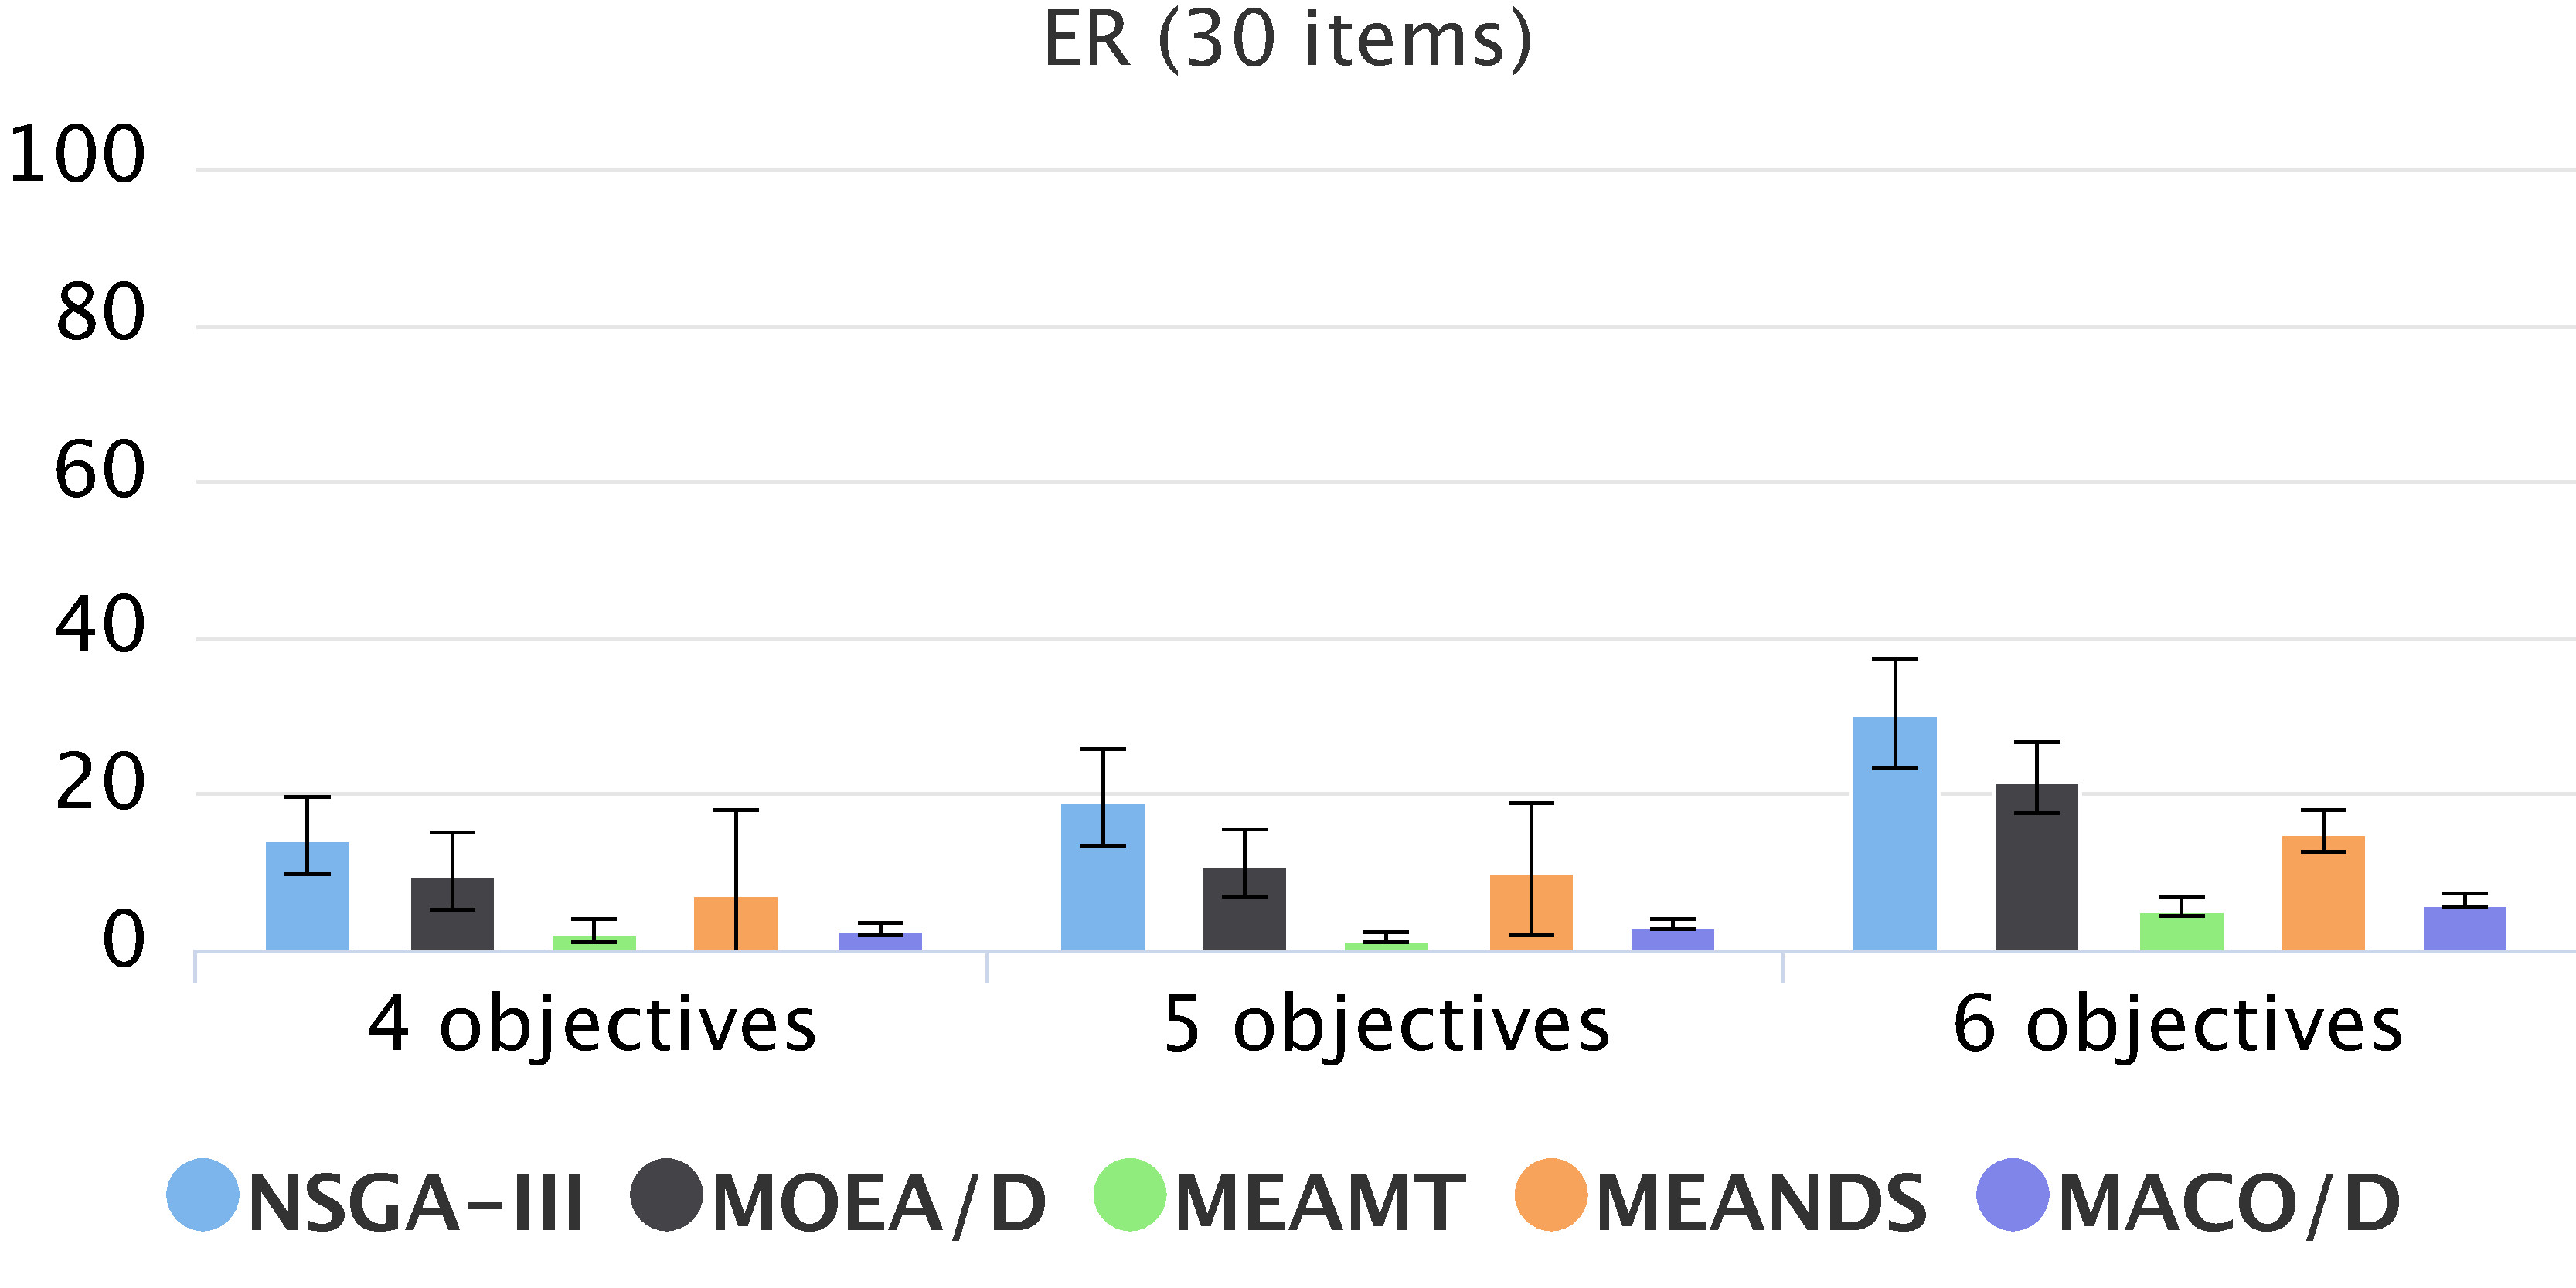
\includegraphics[width=0.5\textwidth]{cap_experimentos/figs/etapa3/er-mkp-30}
	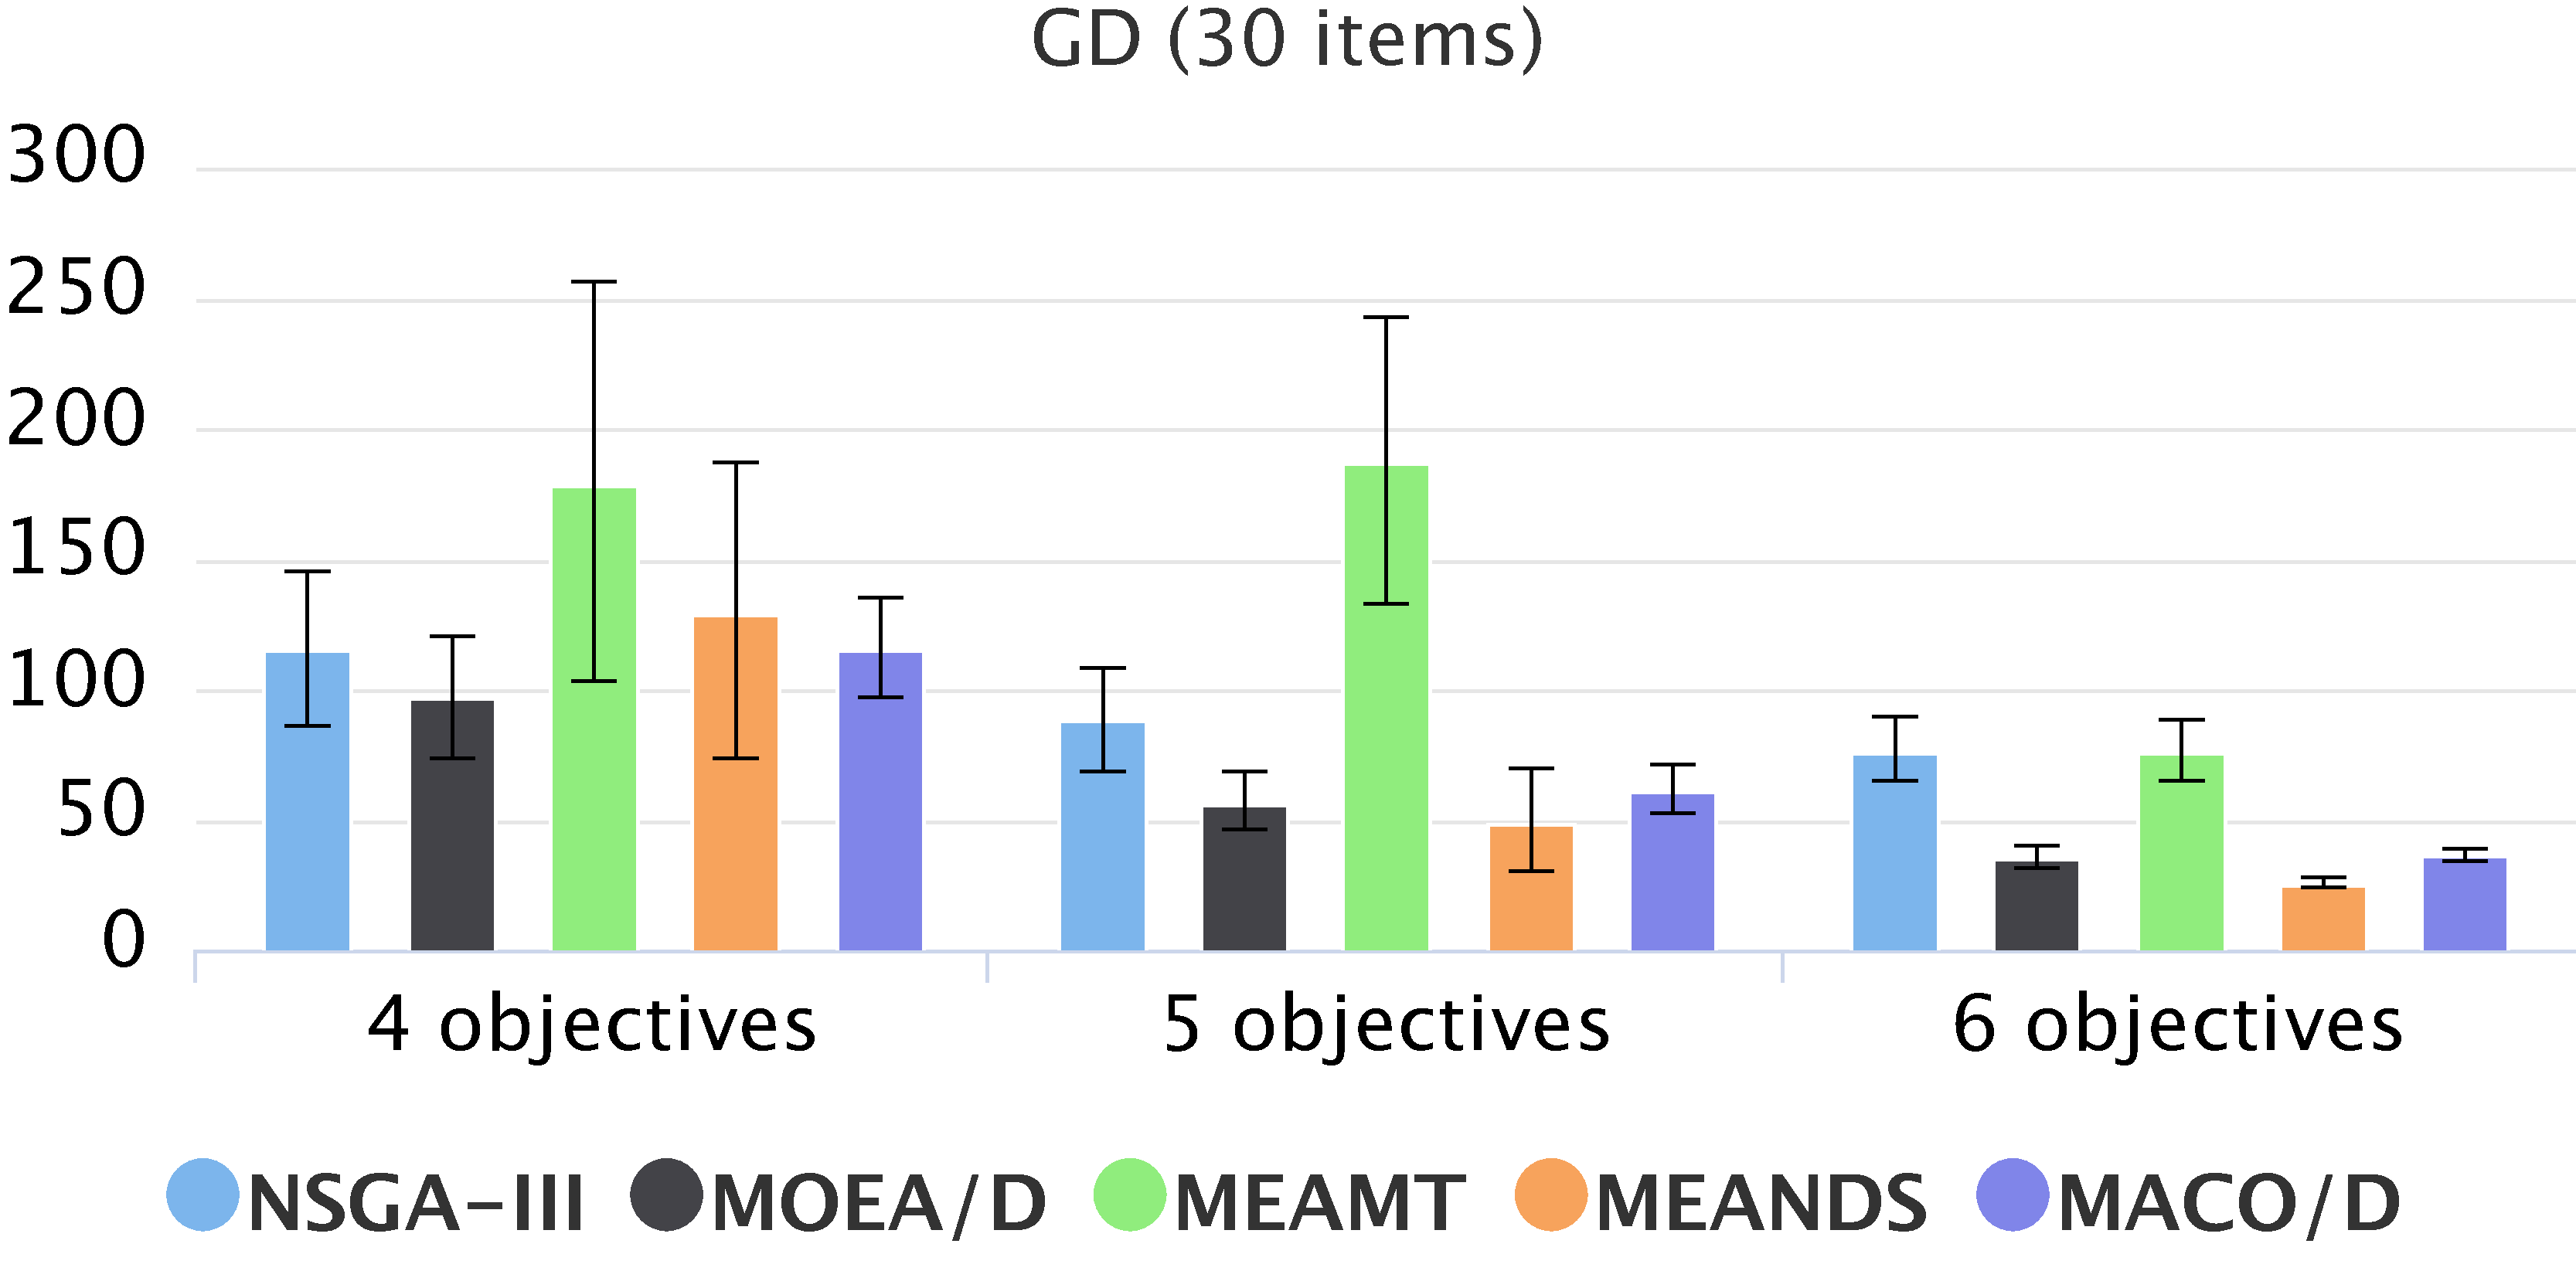
\includegraphics[width=0.5\textwidth]{cap_experimentos/figs/etapa3/gd-mkp-30}
	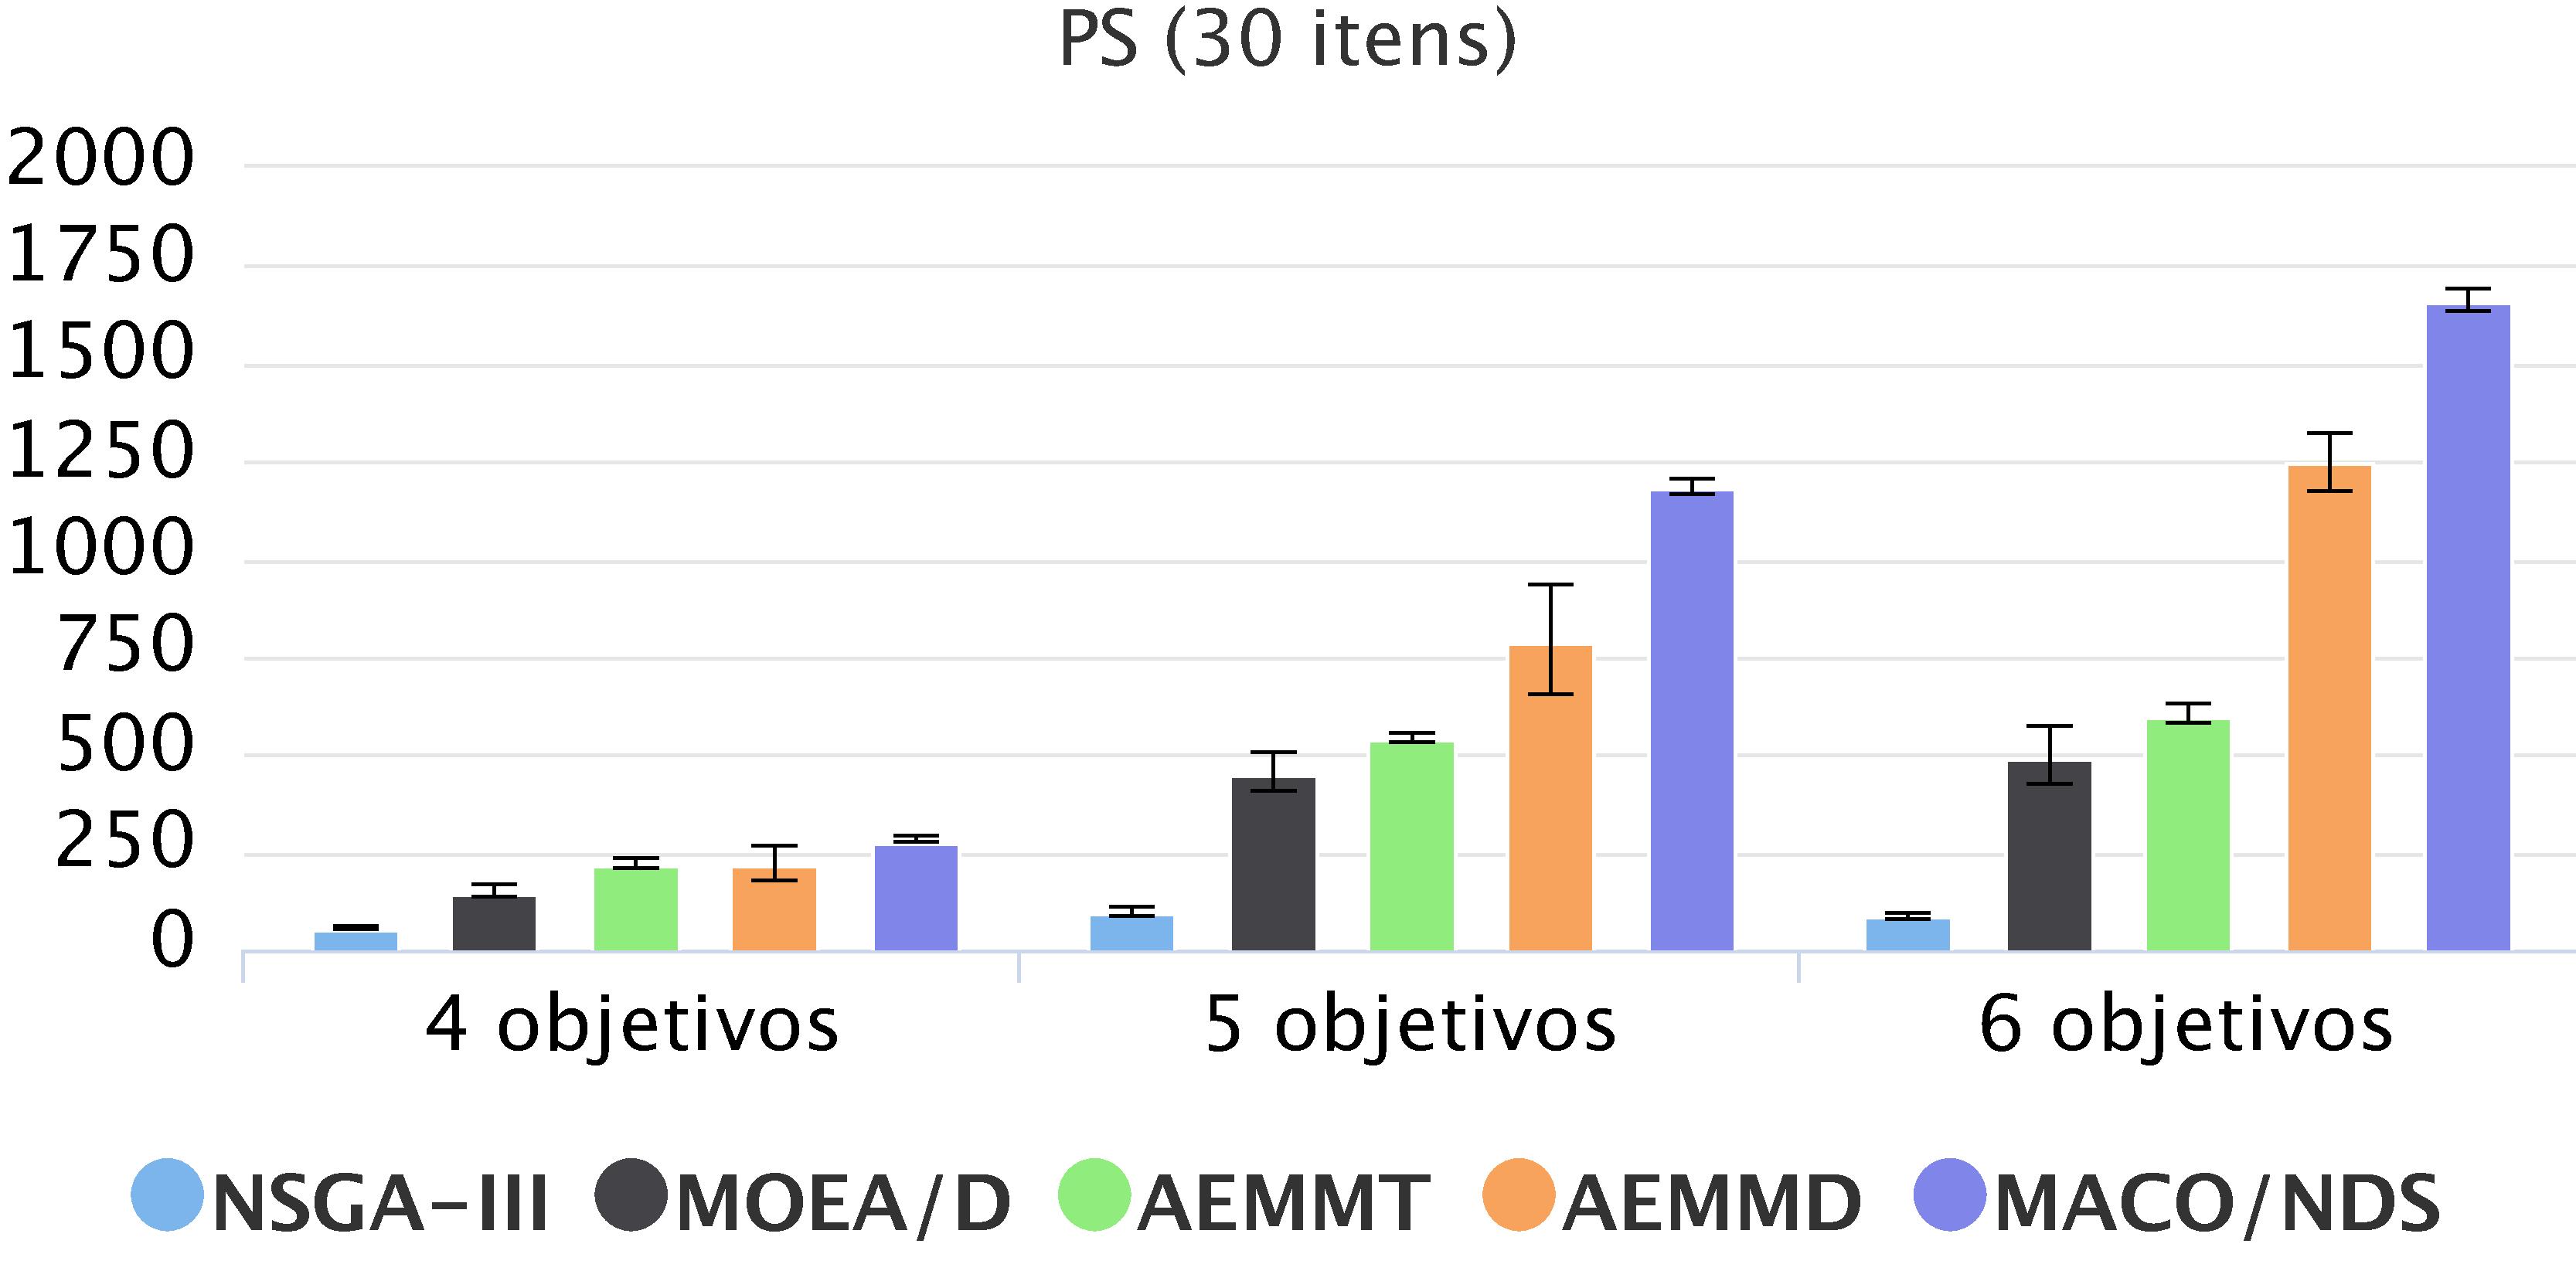
\includegraphics[width=0.5\textwidth]{cap_experimentos/figs/etapa3/ps-mkp-30}
	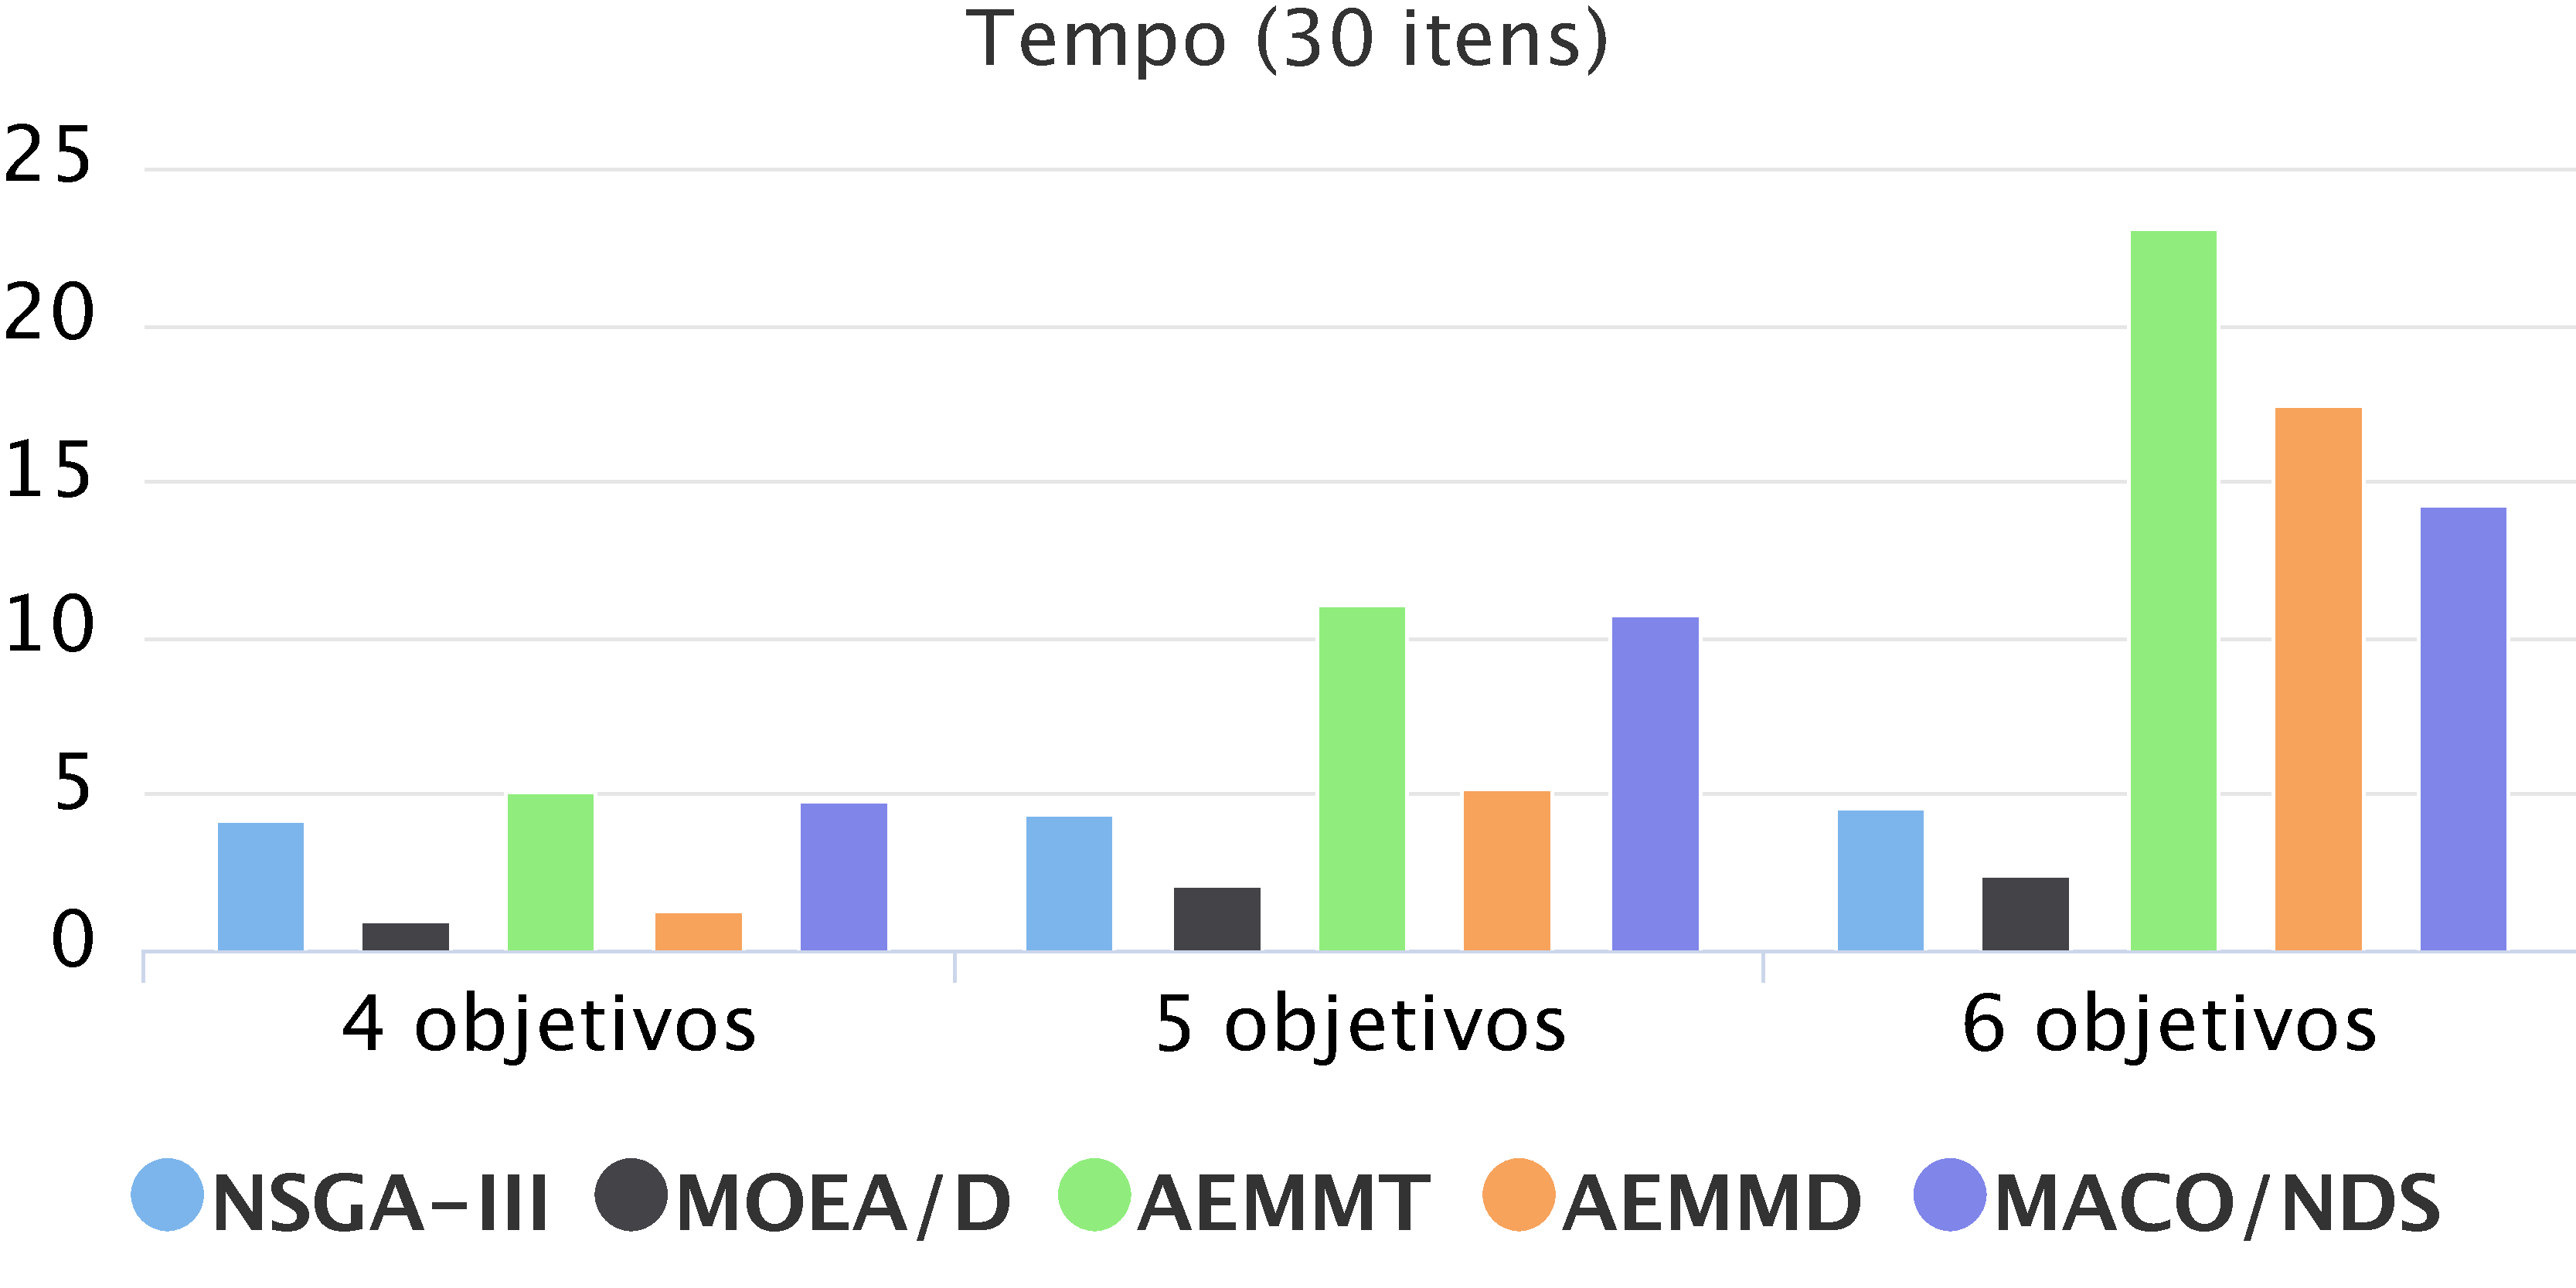
\includegraphics[width=0.5\textwidth]{cap_experimentos/figs/etapa3/time-mkp-30}
	\caption{\label{fig_exp3_pmm_30}Desempenho dos algoritmos na 3ª etapa para o PMM com 30 itens}
\end{figure*}

A \autoref{fig_exp3_pmm_30} retrata a versão mais simples do problema da mochila (30 itens). Nesse cenário, o AEMMT apresenta a menor taxa de erro dentre os algoritmos \textit{many-objective}, seguido pelo MACO/NDS e pelo AEMMD. Considerando a métrica GDp e a formulação com 4 objetivos, os melhores resultados são encontrados pelo MOEA/D, seguido pelo MACO/NDS. Com 5 e 6 objetivos, o AEMMD produz o menor $GD$, sendo acompanhado de perto pelo MACO/NDS. Na métrica $PS$, o MACO/NDS é o algoritmo com melhor desempenho para todas as formulações de objetivo. Na sequência, os algoritmos com os melhores valores de $PS$ são: AEMMD, AEMMT, MOEA/D e NSGA-III. Destre esses algoritmos, o único com um limite fixo no tamanho do Pareto é o NSGA-III. Portanto, é esperado que possua um valor de $PS$ menor. Quanto ao tempo, o MOEA/D é o algoritmo mais rápido, enquanto que o AEMMT é o mais lento. No geral, o MACO/NDS apresentou o melhor equilíbrio entre as métricas de desempenho, revelando-se a melhor opção, nessa instância (30 itens), para formulações com muitos objetivos. Além disso, o MACO/NDS apresenta os menores desvios padrões, ou seja, é o método que prova maior segurança quanto à qualidade de suas soluções, independentemente da execução.

\begin{figure*}[!htbp]	
	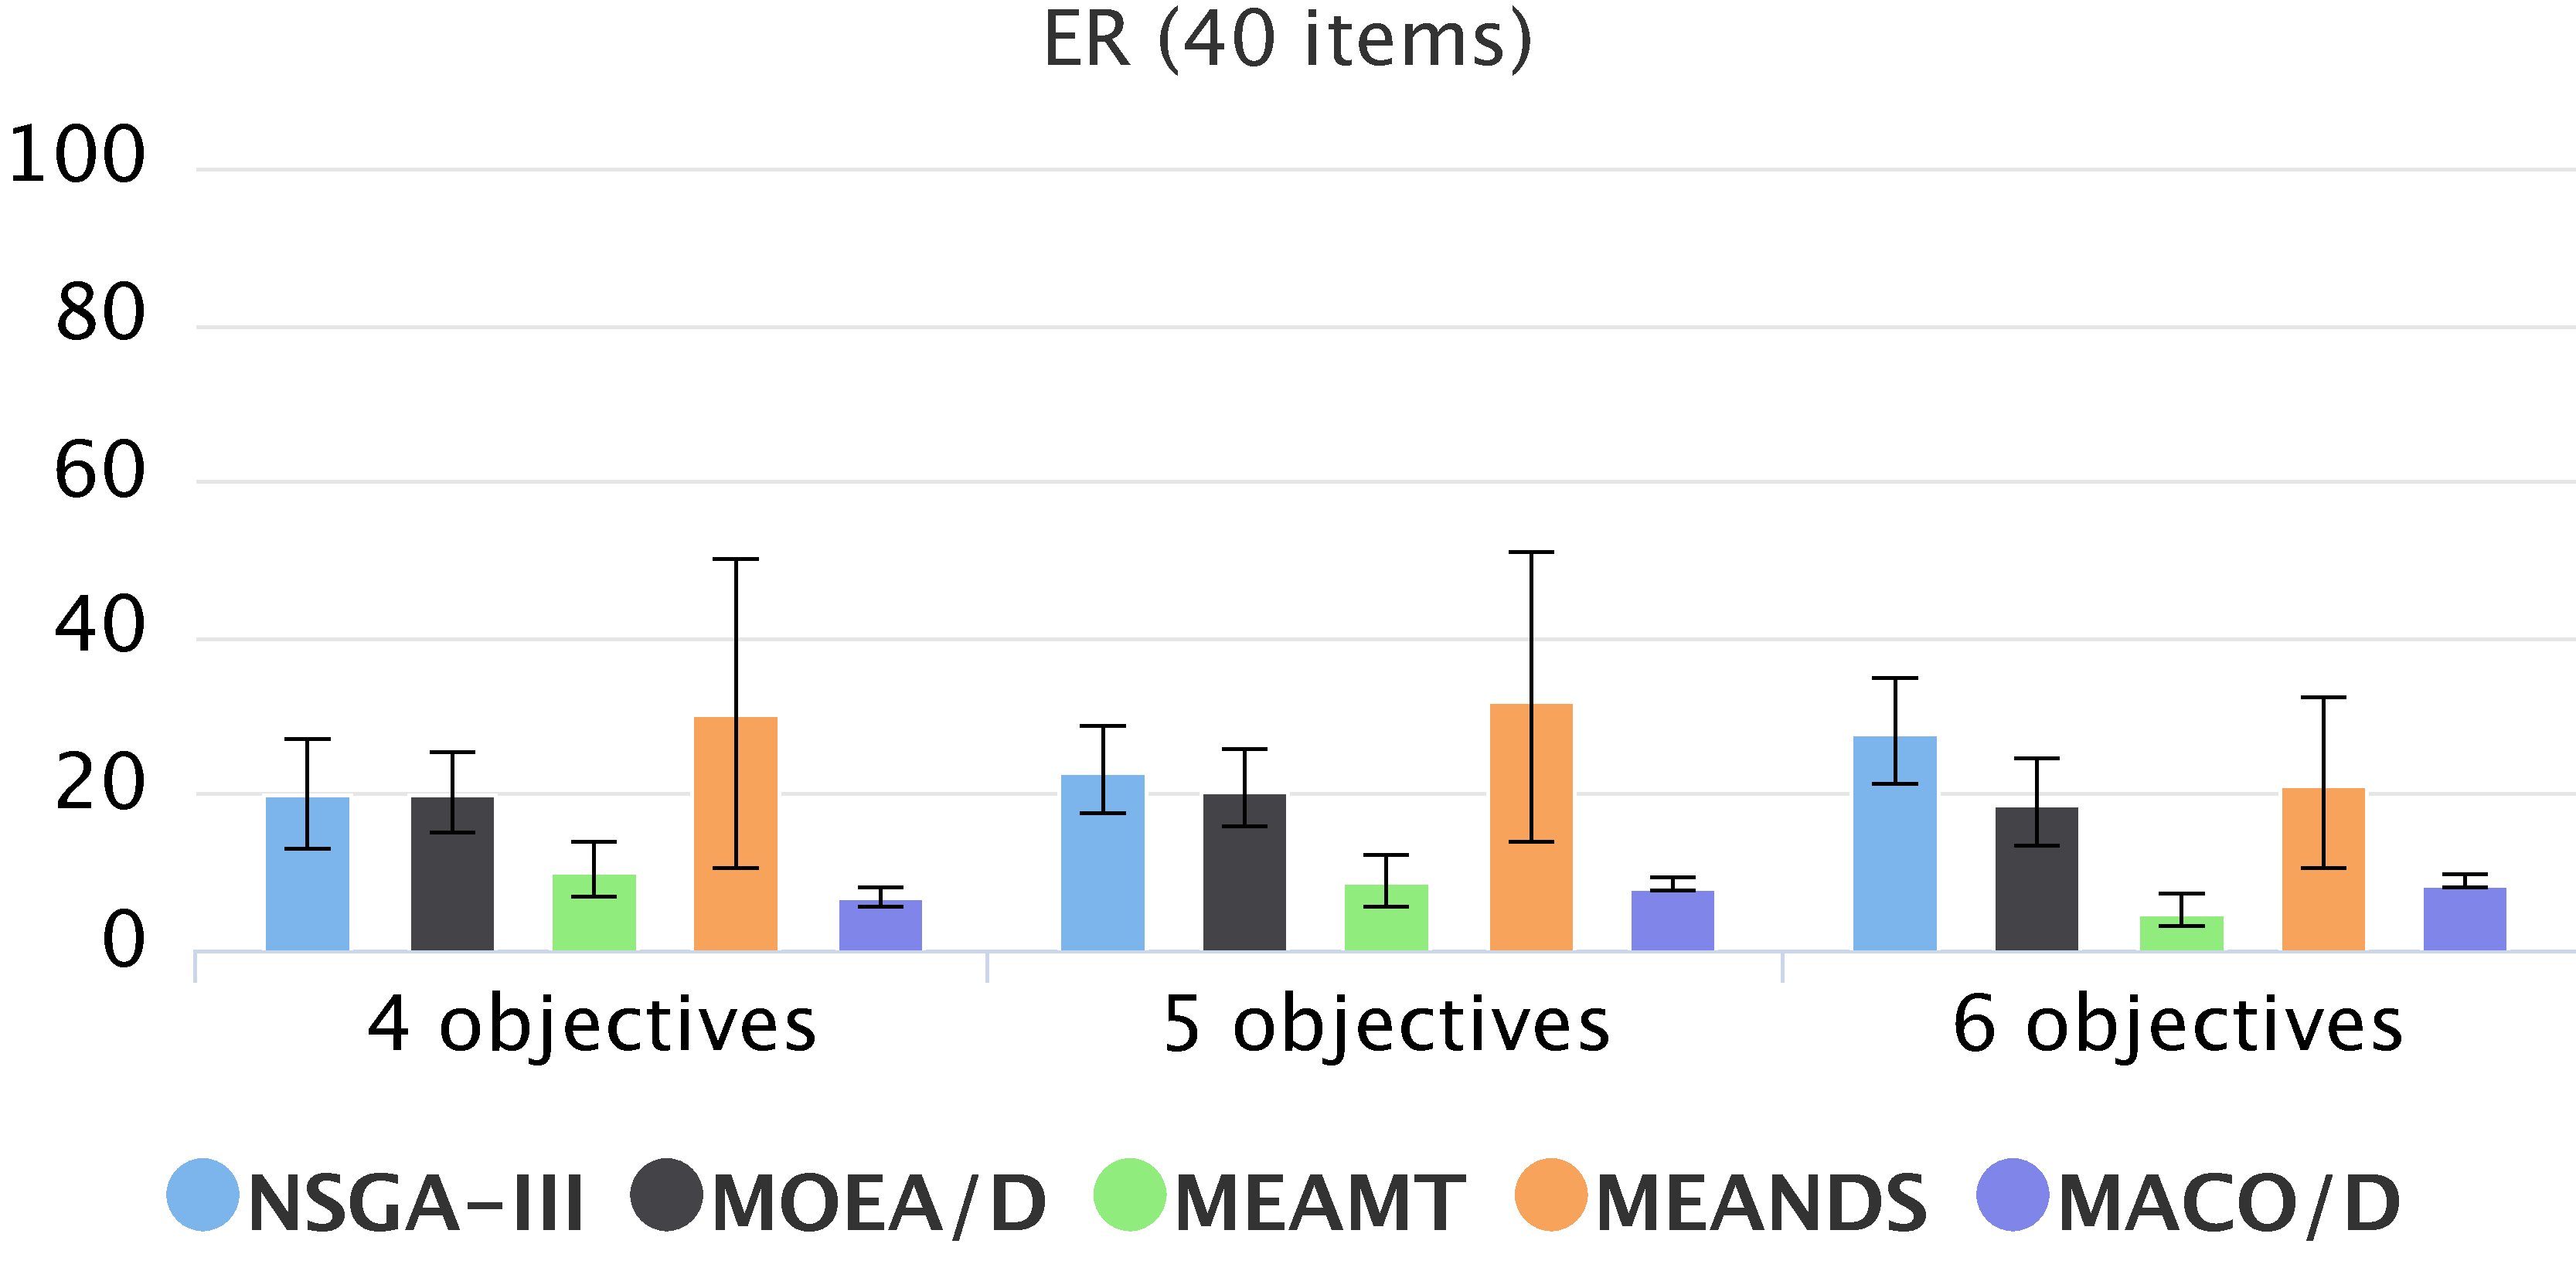
\includegraphics[width=0.5\textwidth]{cap_experimentos/figs/etapa3/er-mkp-40}
	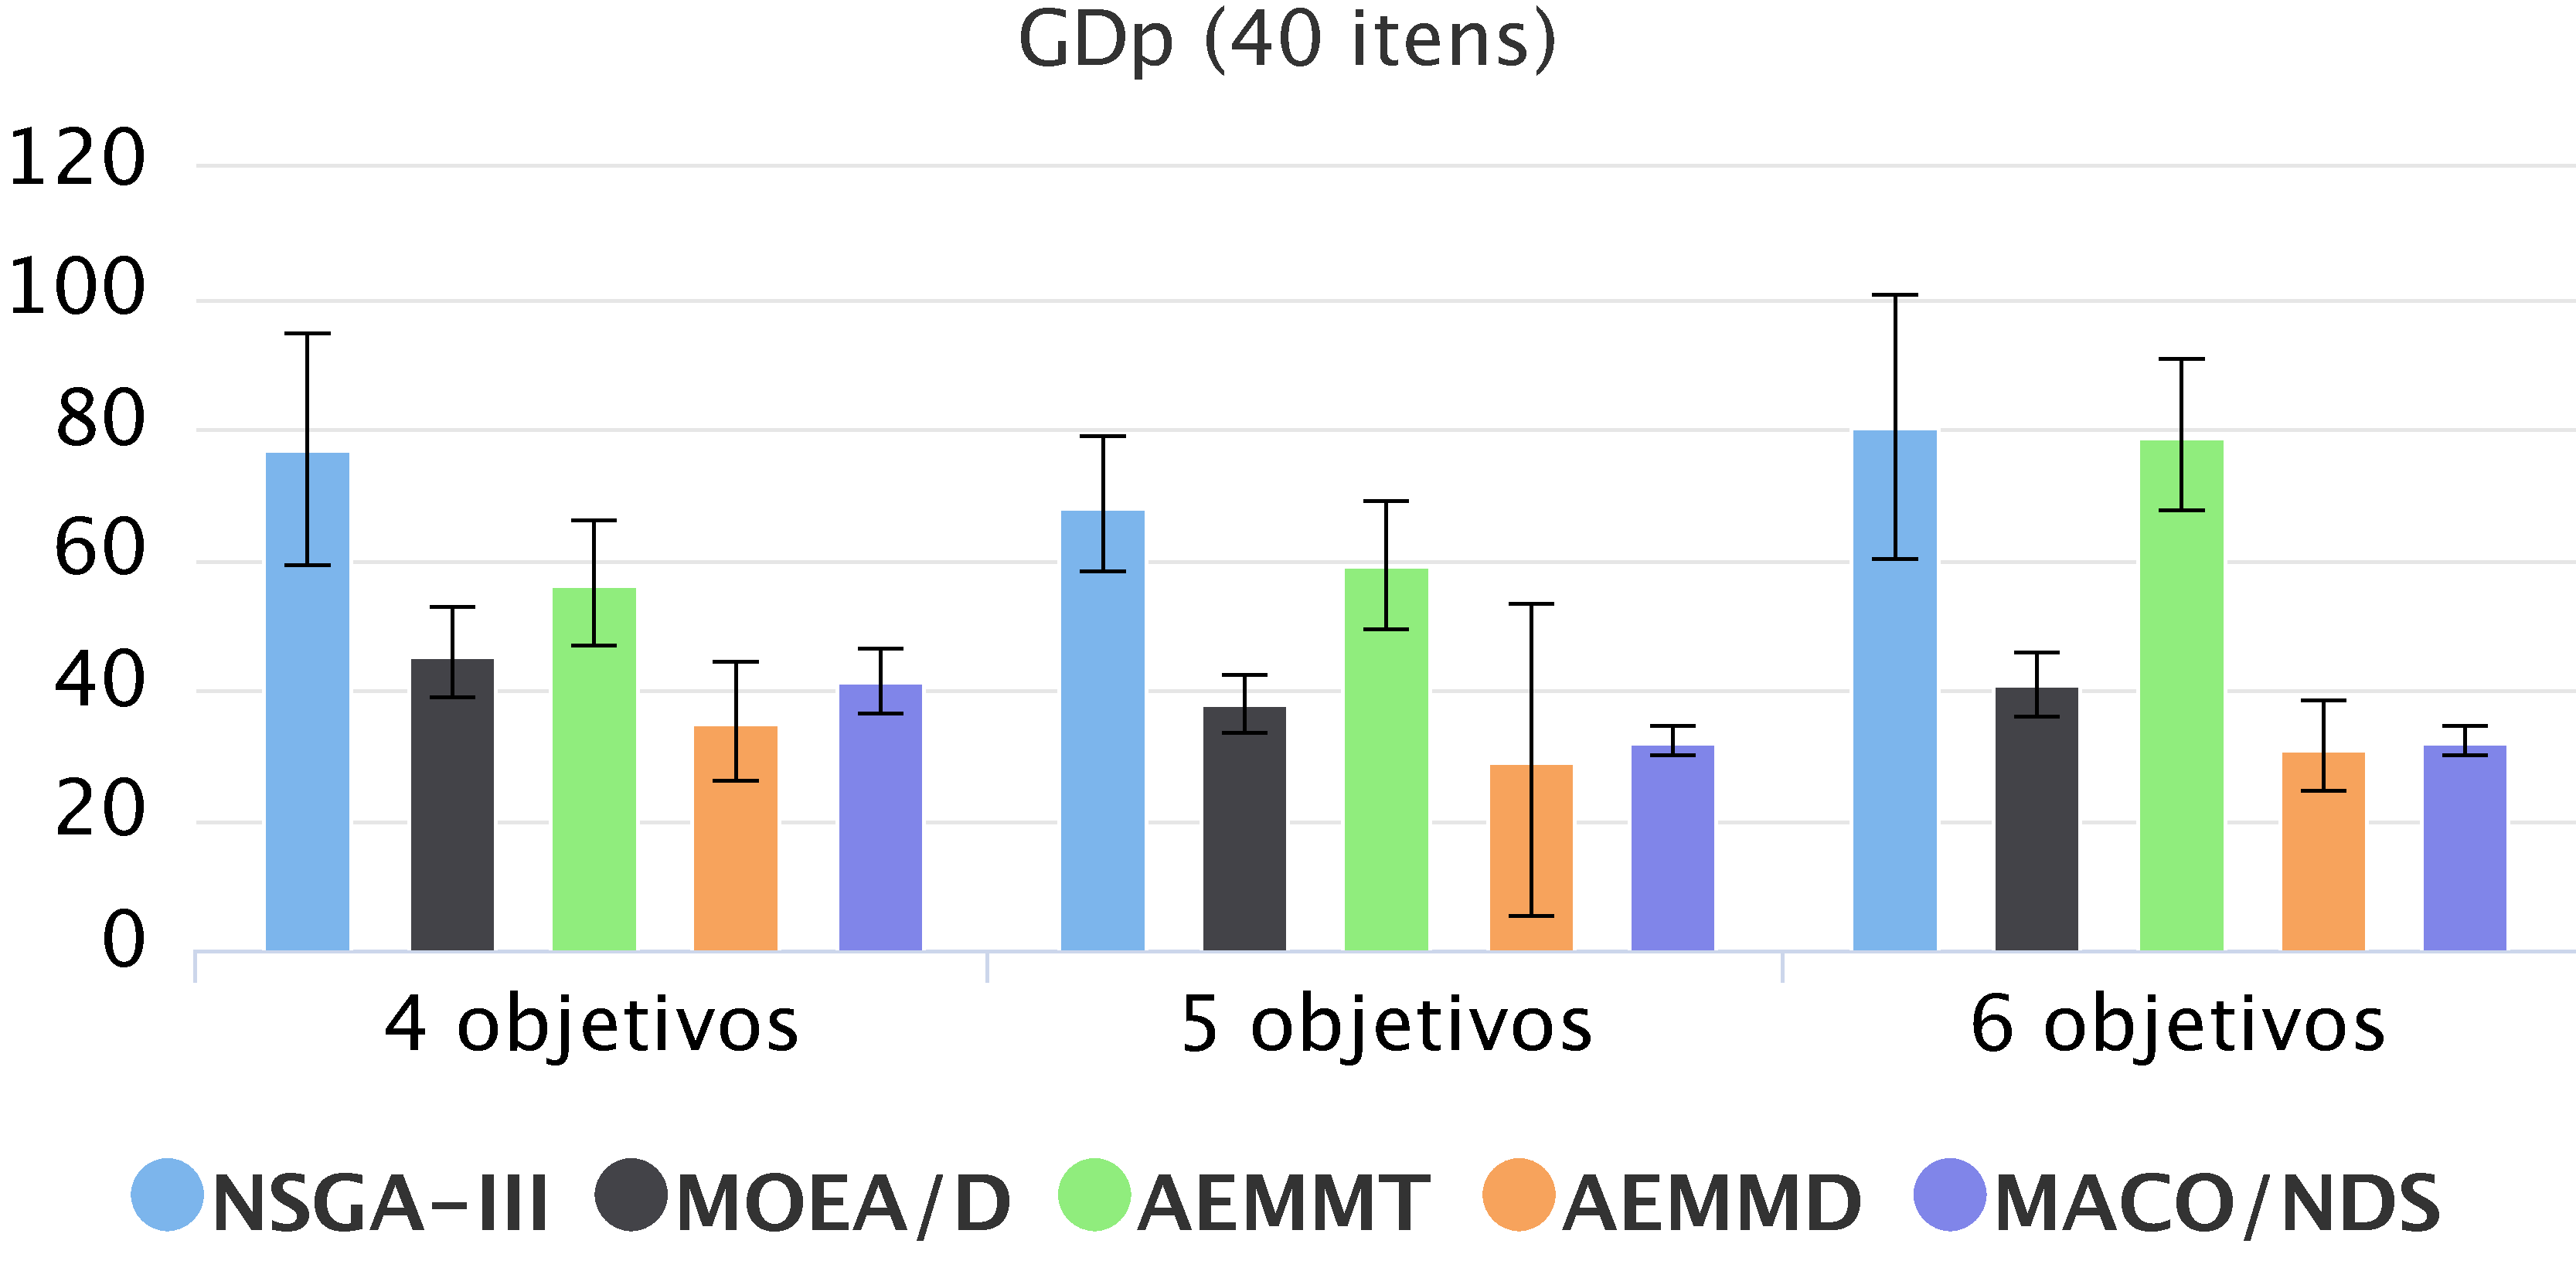
\includegraphics[width=0.5\textwidth]{cap_experimentos/figs/etapa3/gd-mkp-40}
	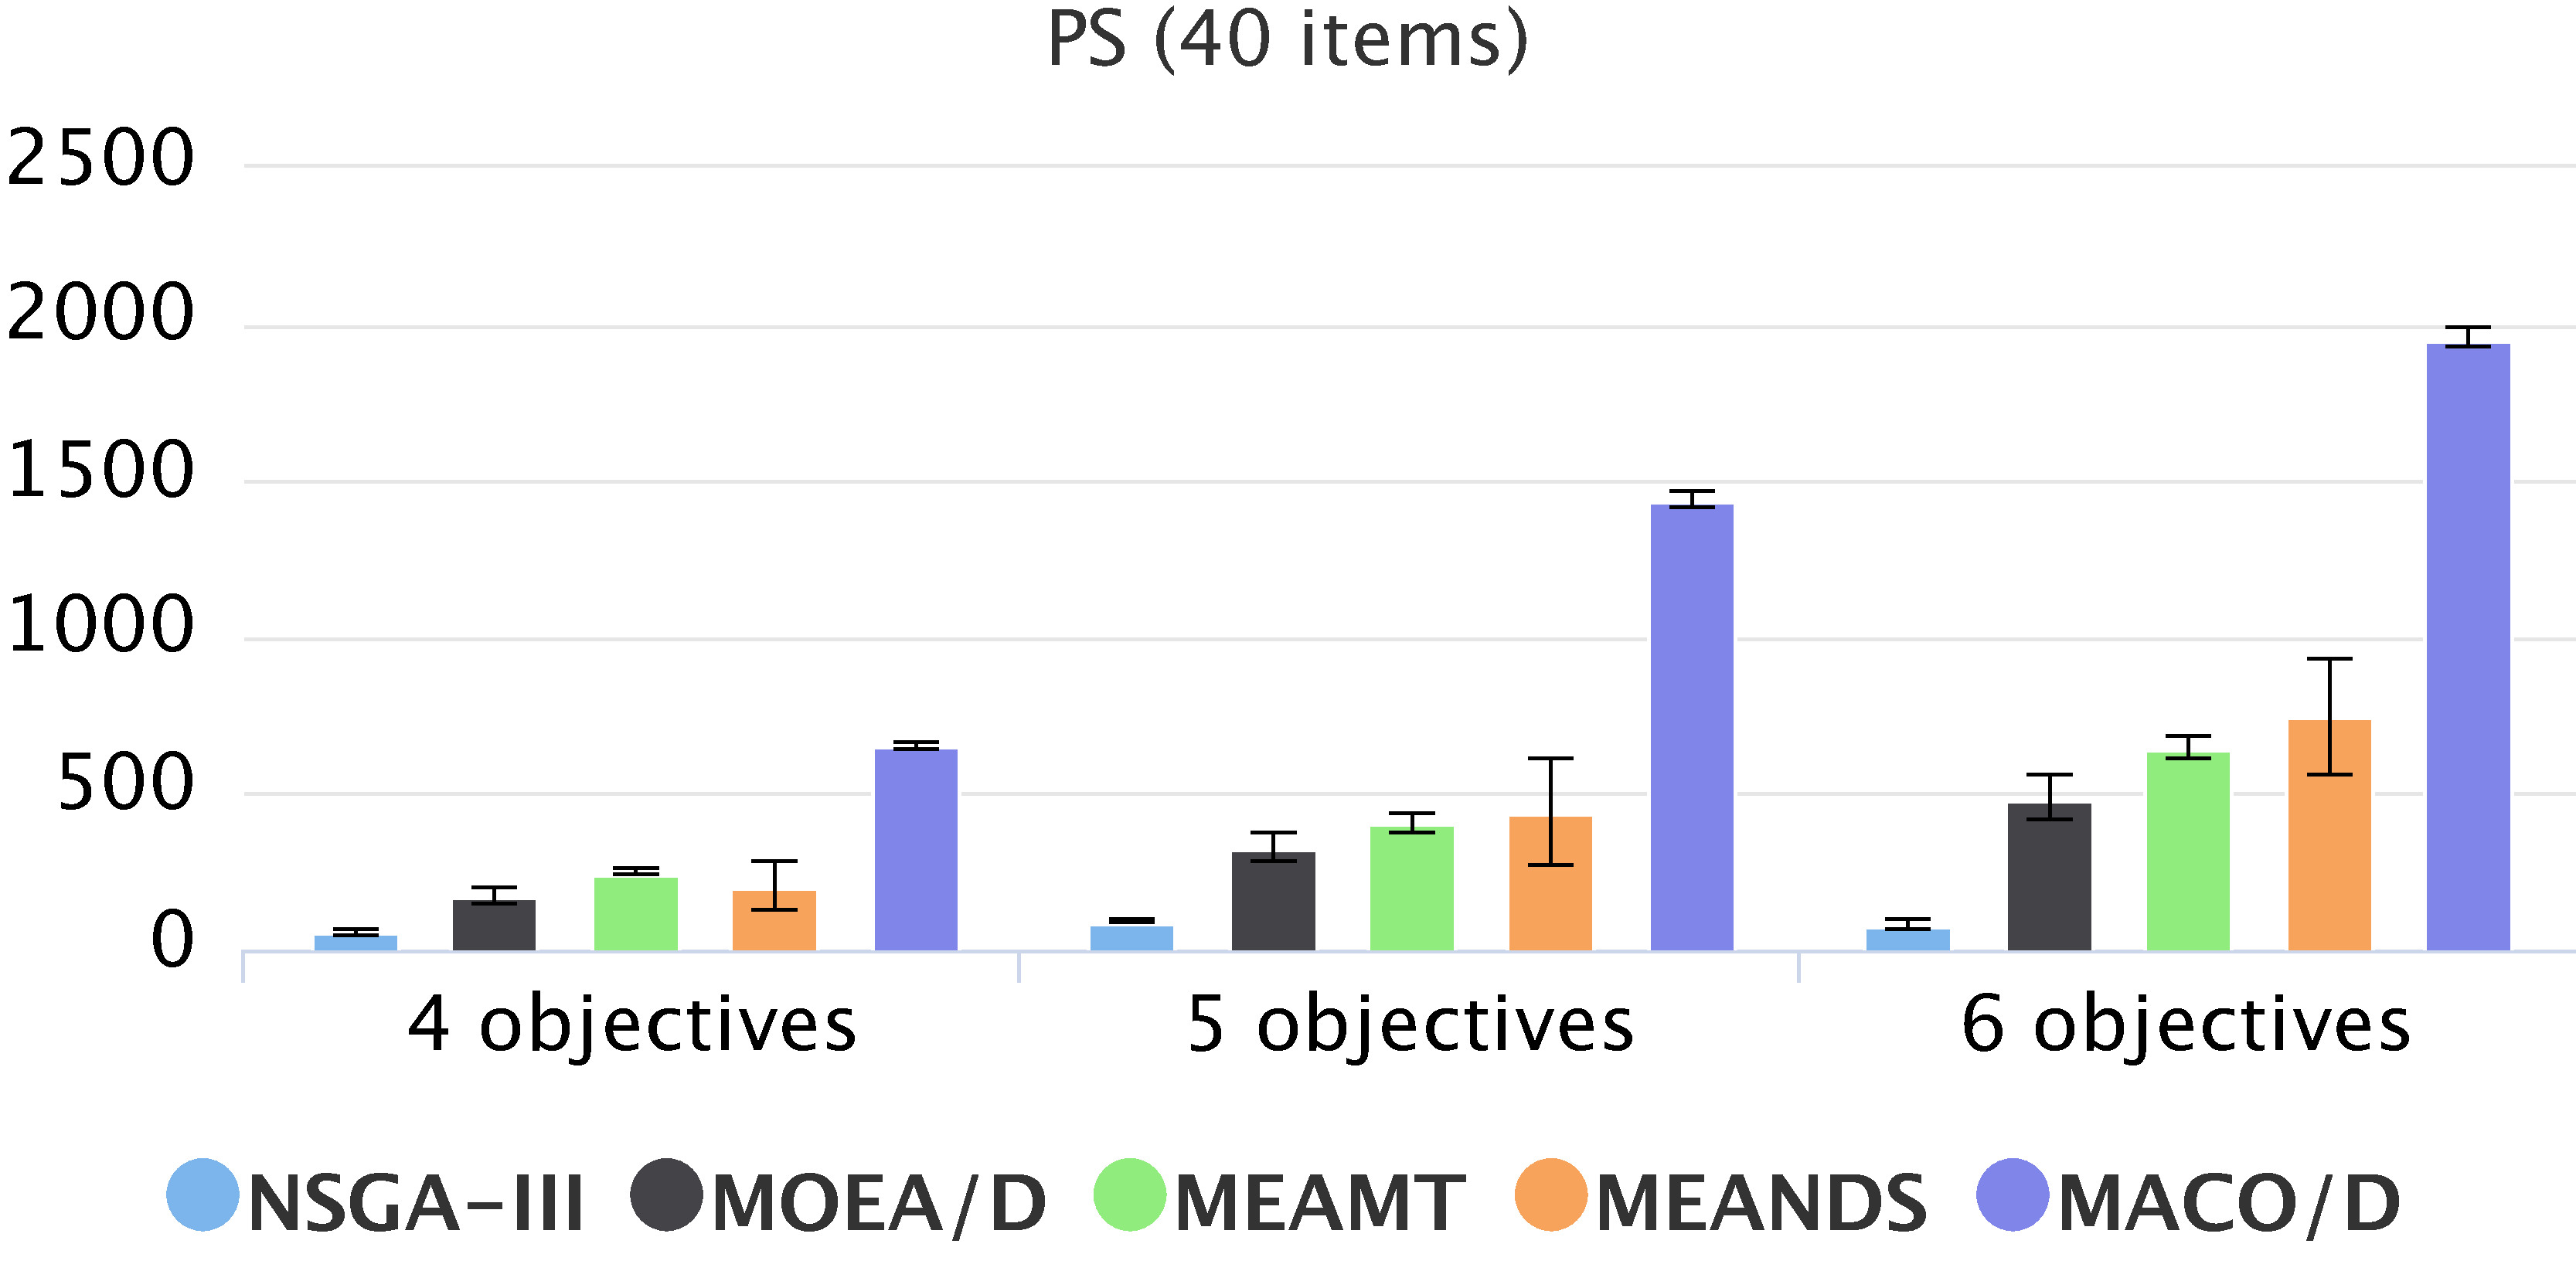
\includegraphics[width=0.5\textwidth]{cap_experimentos/figs/etapa3/ps-mkp-40}
	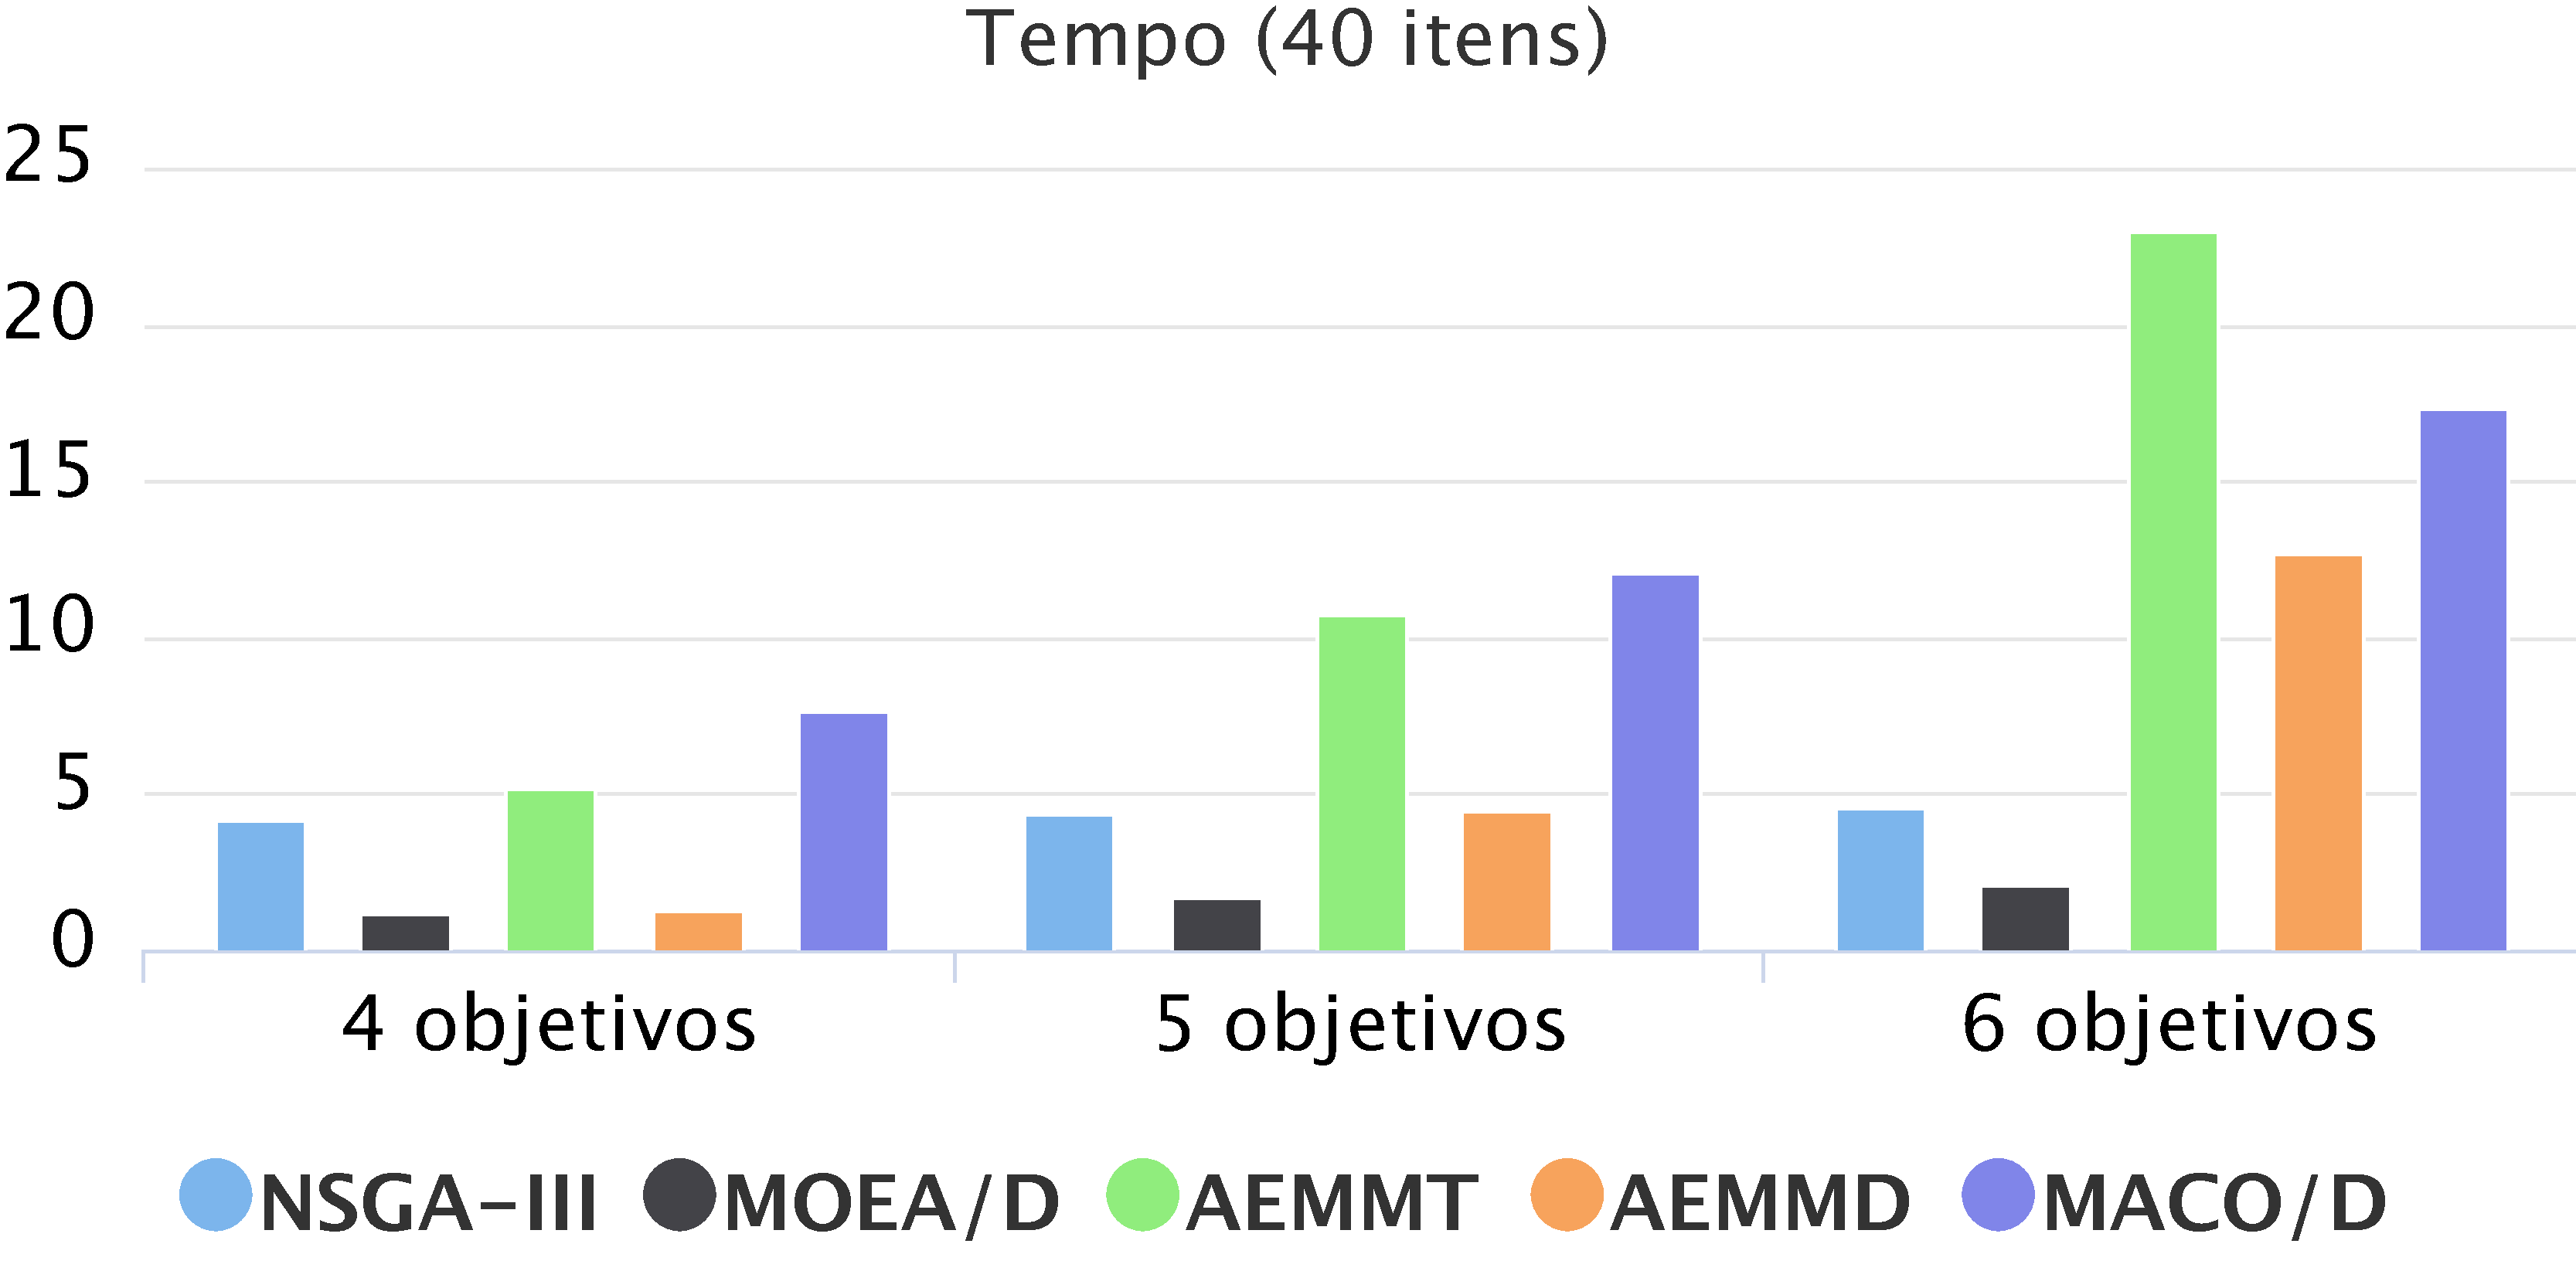
\includegraphics[width=0.5\textwidth]{cap_experimentos/figs/etapa3/time-mkp-40}
	\caption{\label{fig_exp3_pmm_40}Desempenho dos algoritmos na 3ª etapa para o PMM com 40 itens}
\end{figure*}

Os resultados obtidos para o PMM de 40 itens é apresentado na \autoref{fig_exp3_pmm_40}. O AEMMT e o MACO/NDS apresentam as menores taxas de erro, sendo que o MACO/NDS é melhor para 4 e 5 objetivos (6,9\% e 8,4\%, respectivamente), enquanto o AEMMT obtém o melhor resultado para 6 objetivos (5,1\% contra 8,7\% do MACO/NDS). Os melhores valores de $GDp$ foram encontrados pelo AEMMD e MACO/NDS, sendo o primeiro um pouco melhor que o segundo. Em contrapartida, o AEMMD apresenta uma alta variação nos resultados, indicando que algumas execuções produzem soluções muito próximas do Pareto enquanto outras nem tanto. Considerando o tamanho dos Paretos encontrados ($PS$), novamente o MACO/NDS retorna os melhores valores independentemente da formulação de objetivos. Em termos do tempo médio de execução, o MOEA/D é o algoritmo mais rápido (5,2 segundos ao somar o tempo das 3 formulações de objetivos), enquanto o AEMMT e o MACO/NDS são os mais lentos (39 e 37,2 segundos, ao somar o tempo das 3 formulações de objetivos, respectivamente).

\begin{figure*}[!htbp]
	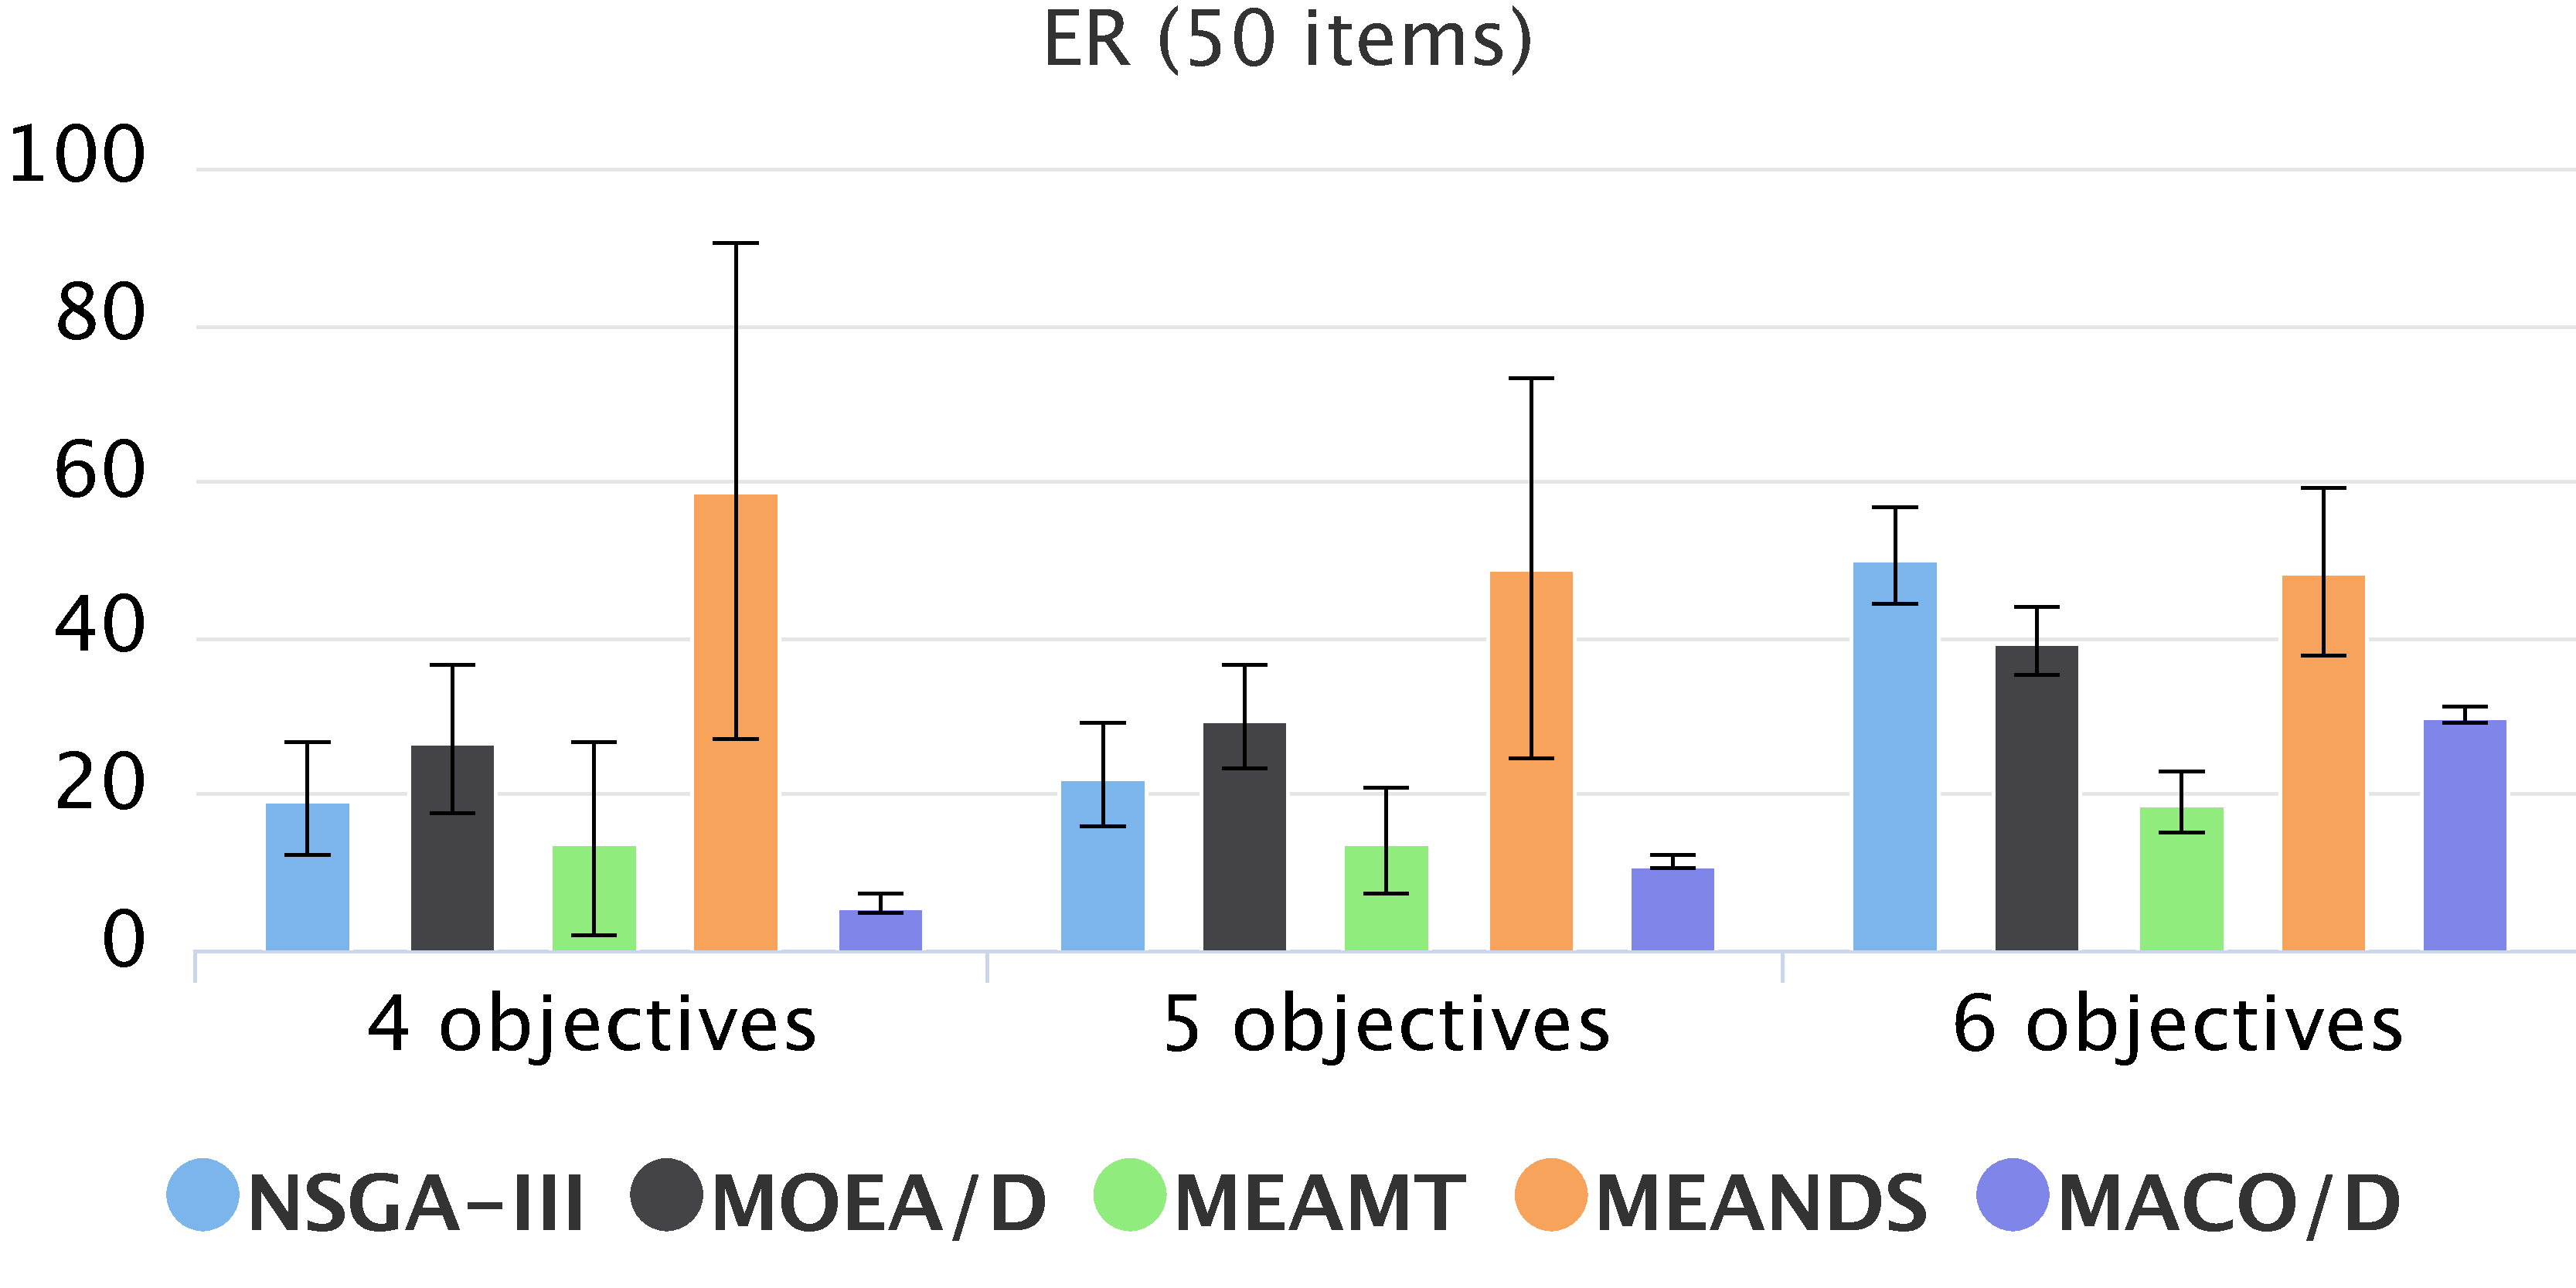
\includegraphics[width=0.5\textwidth]{cap_experimentos/figs/etapa3/er-mkp-50}
	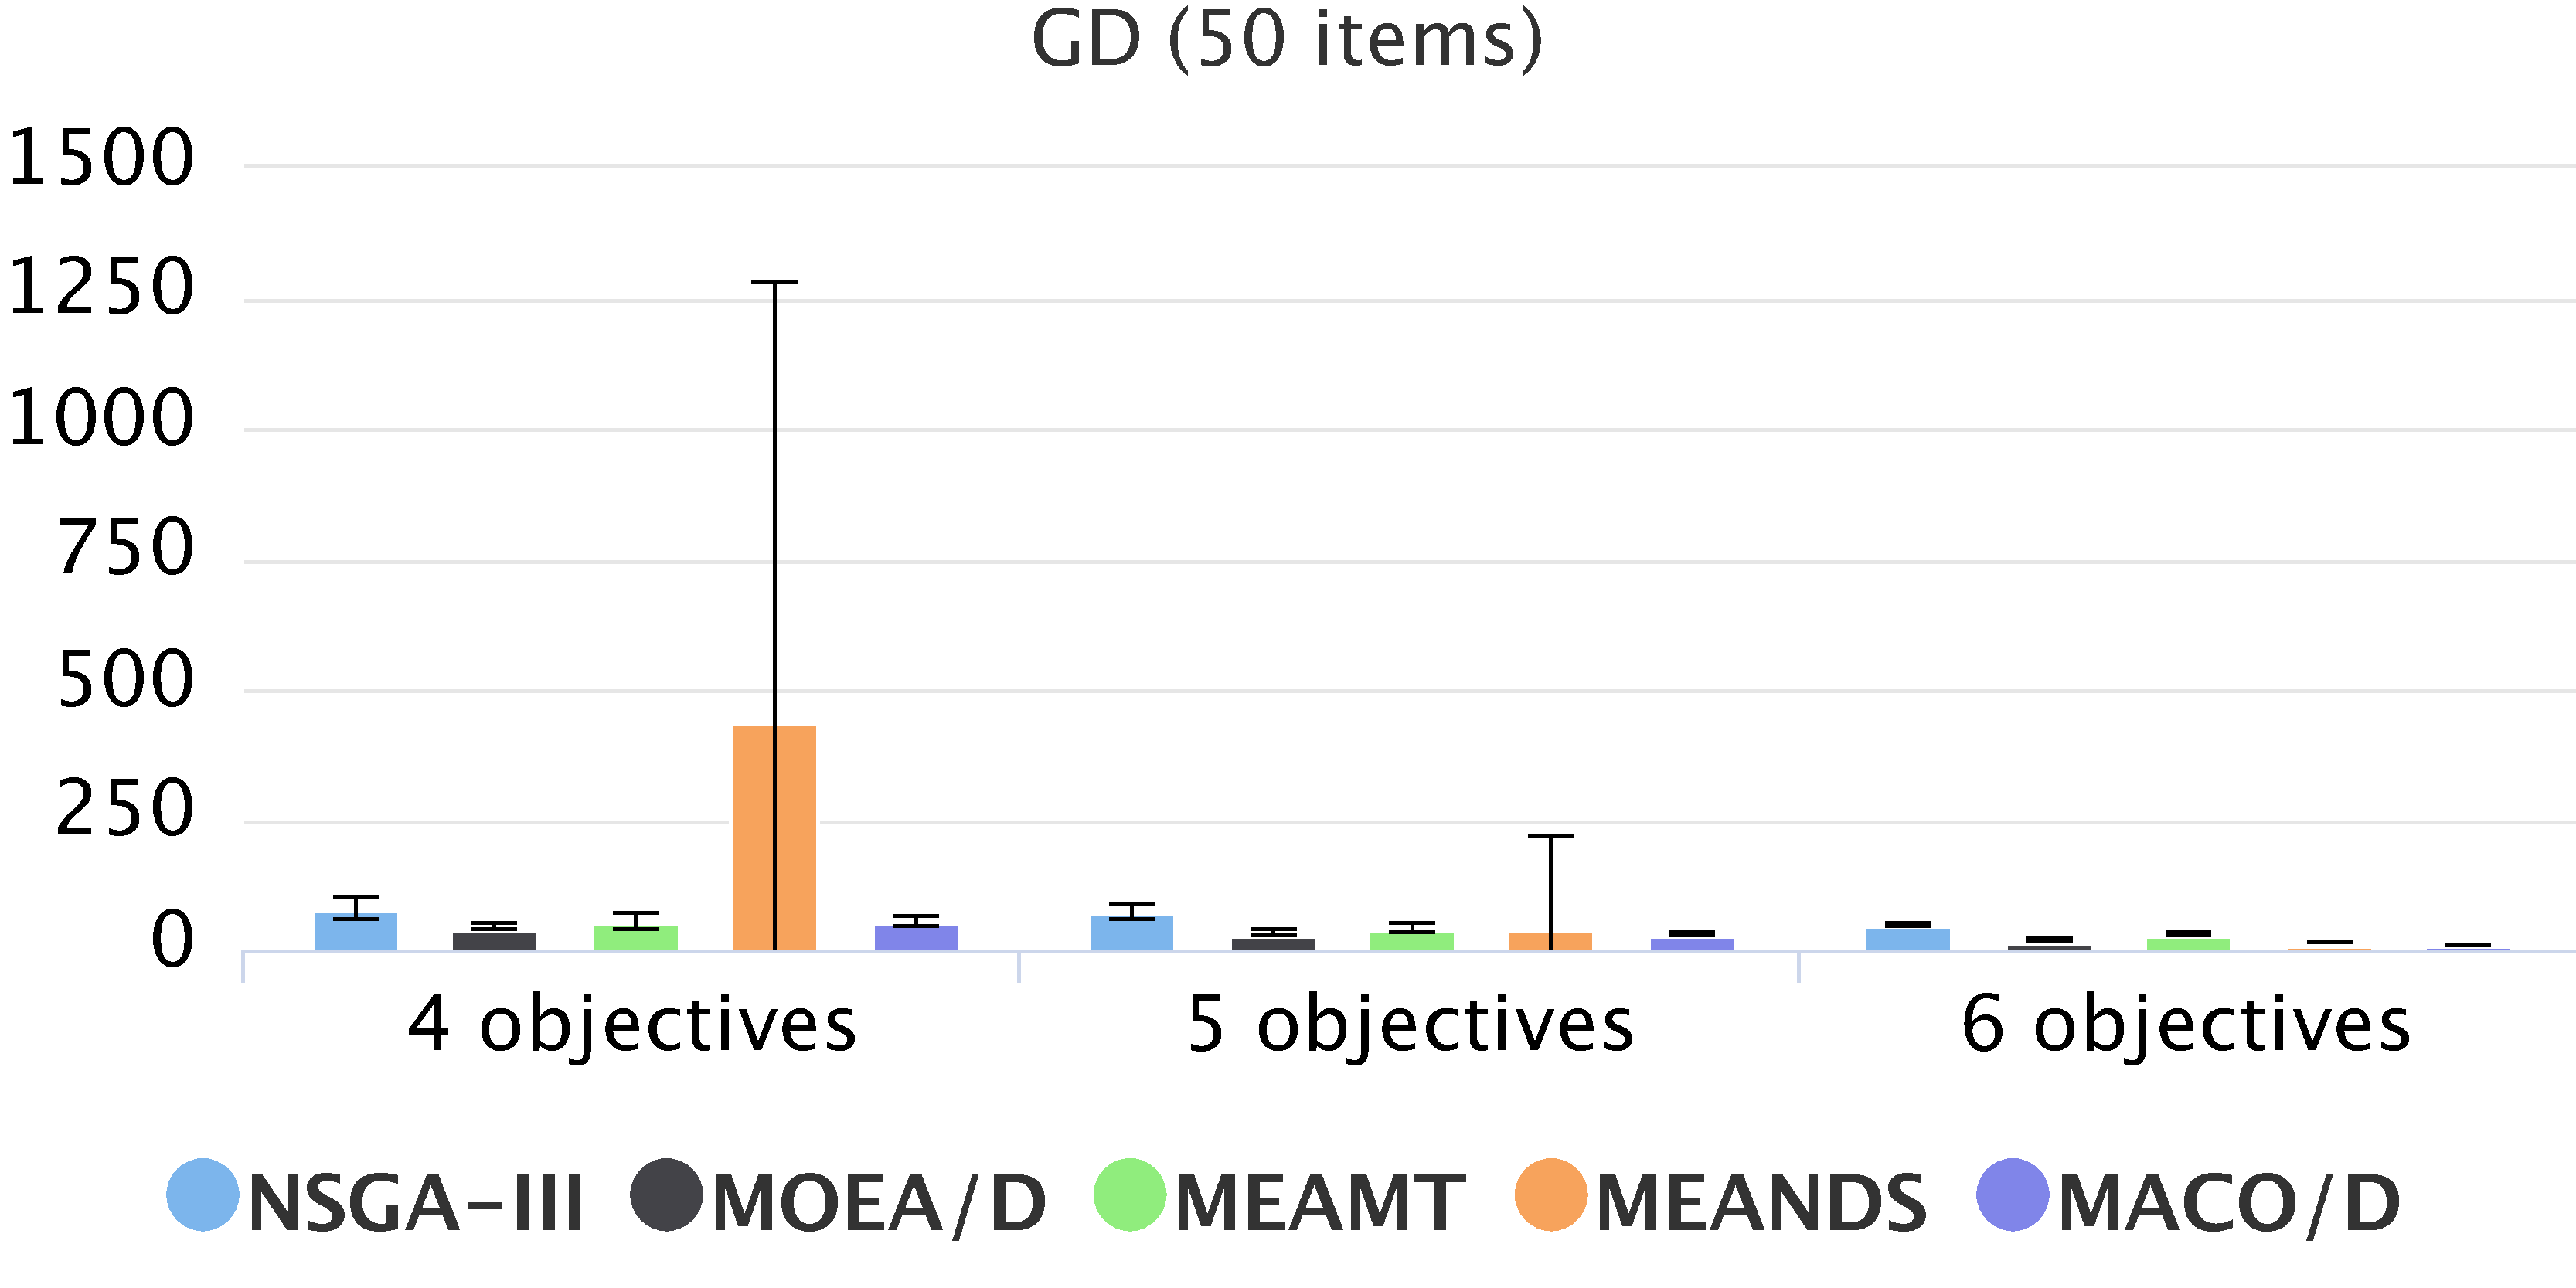
\includegraphics[width=0.5\textwidth]{cap_experimentos/figs/etapa3/gd-mkp-50}
	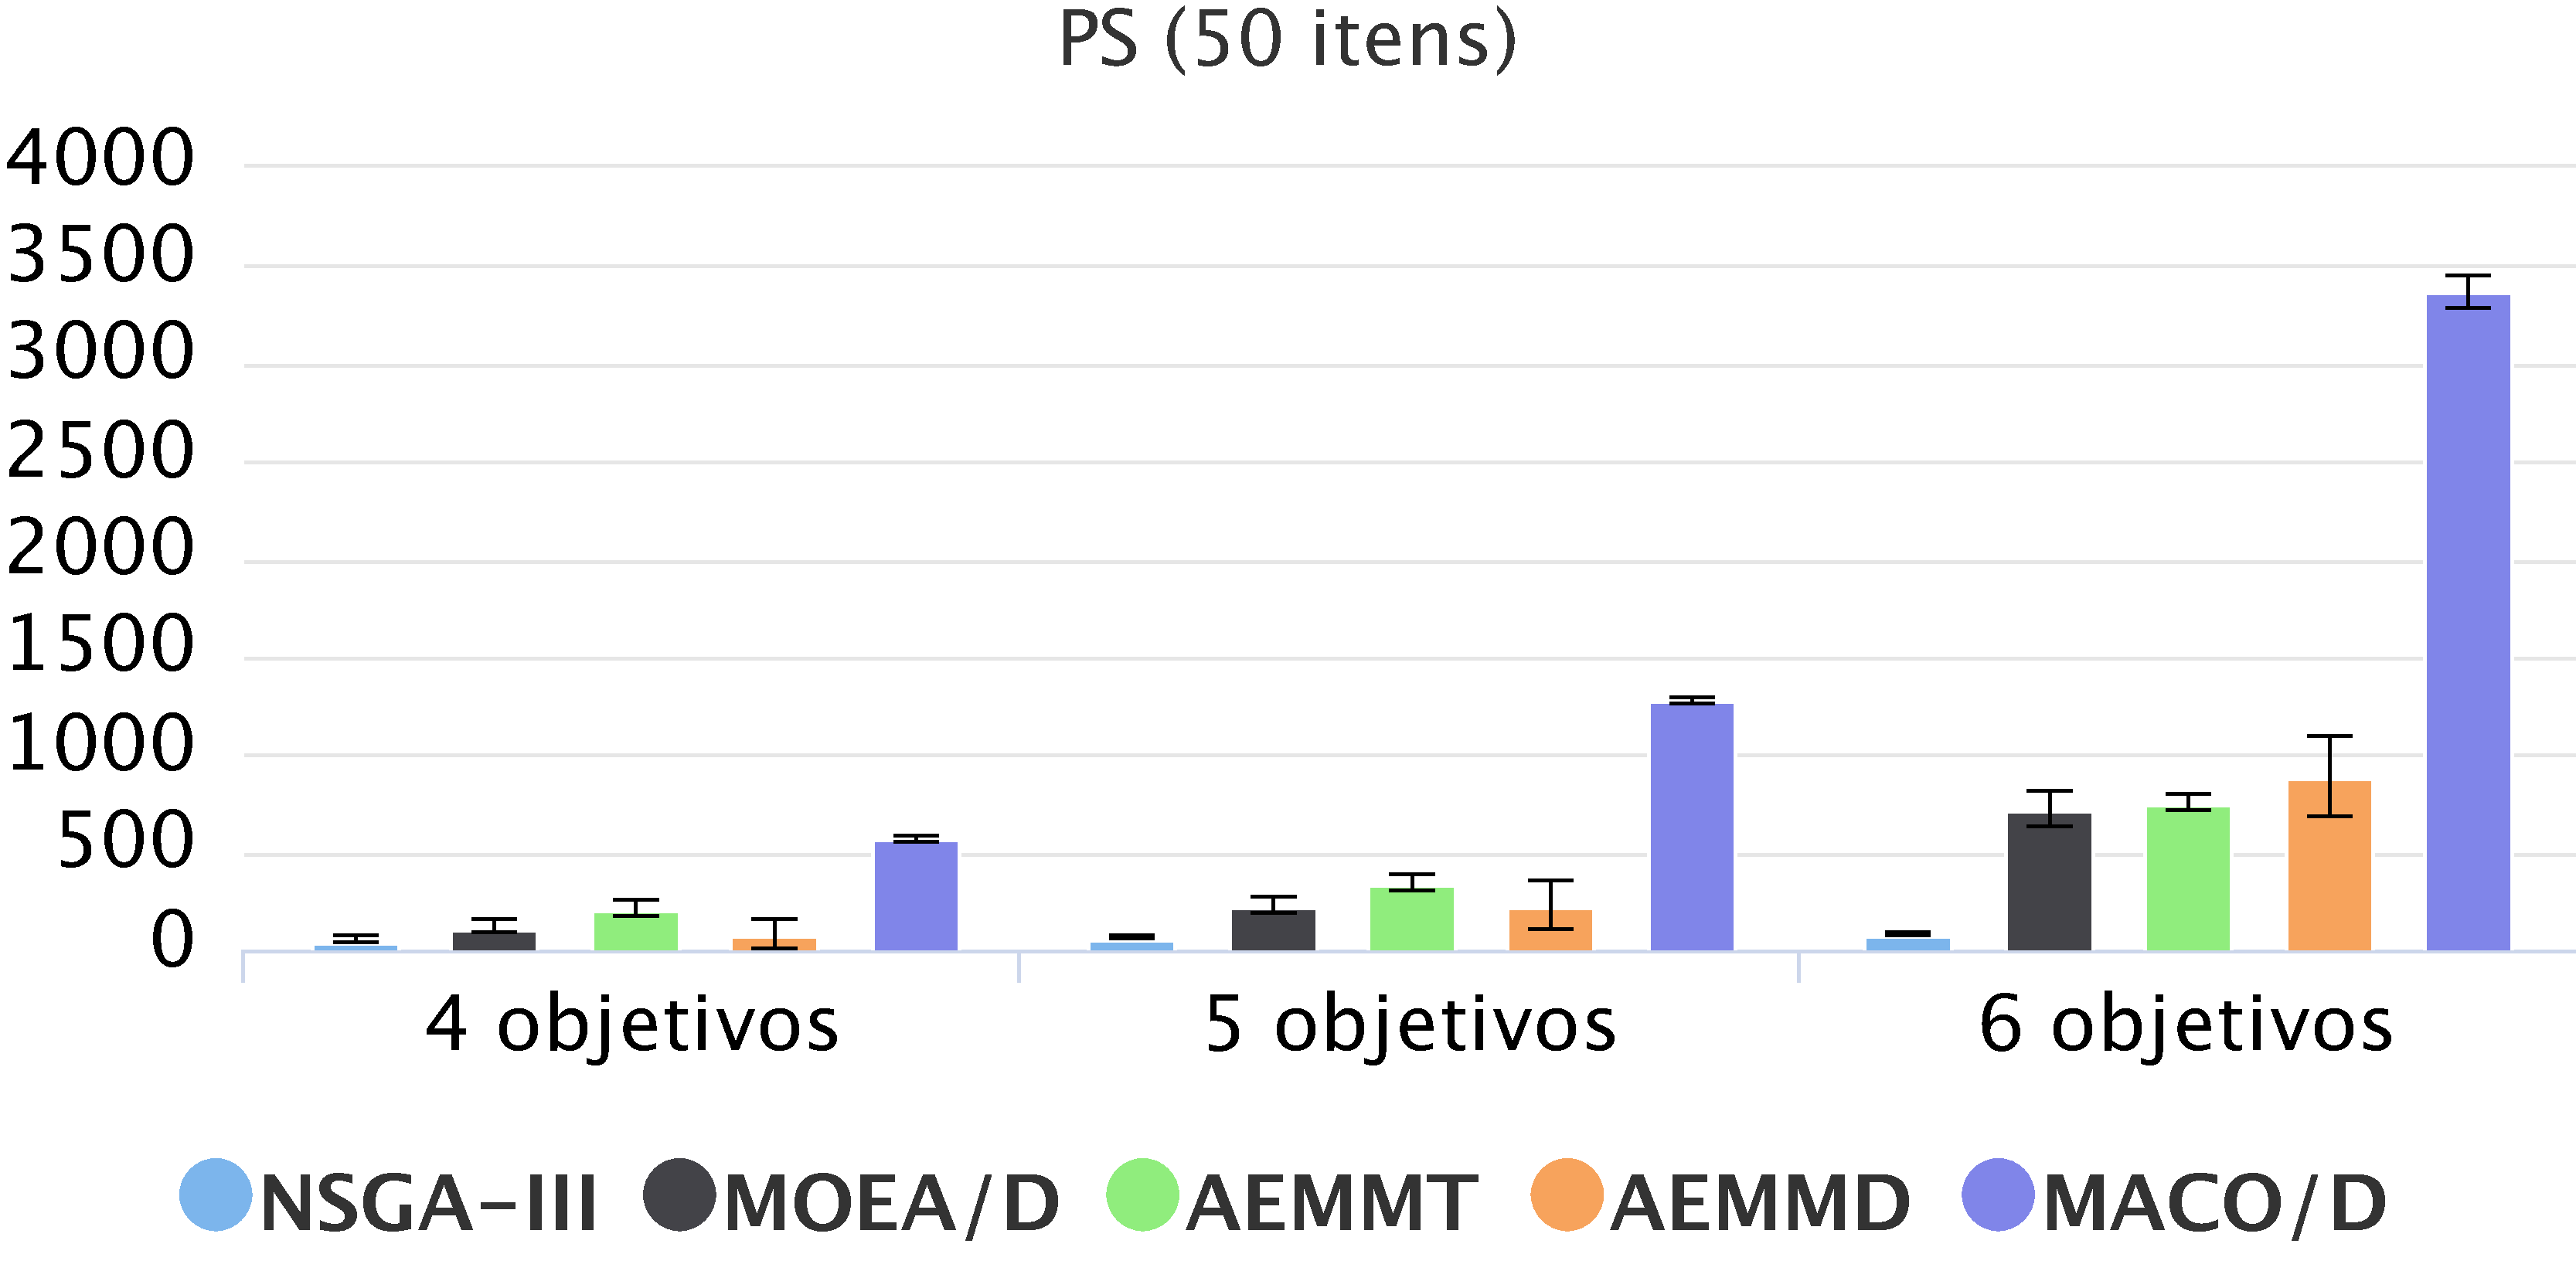
\includegraphics[width=0.5\textwidth]{cap_experimentos/figs/etapa3/ps-mkp-50}
	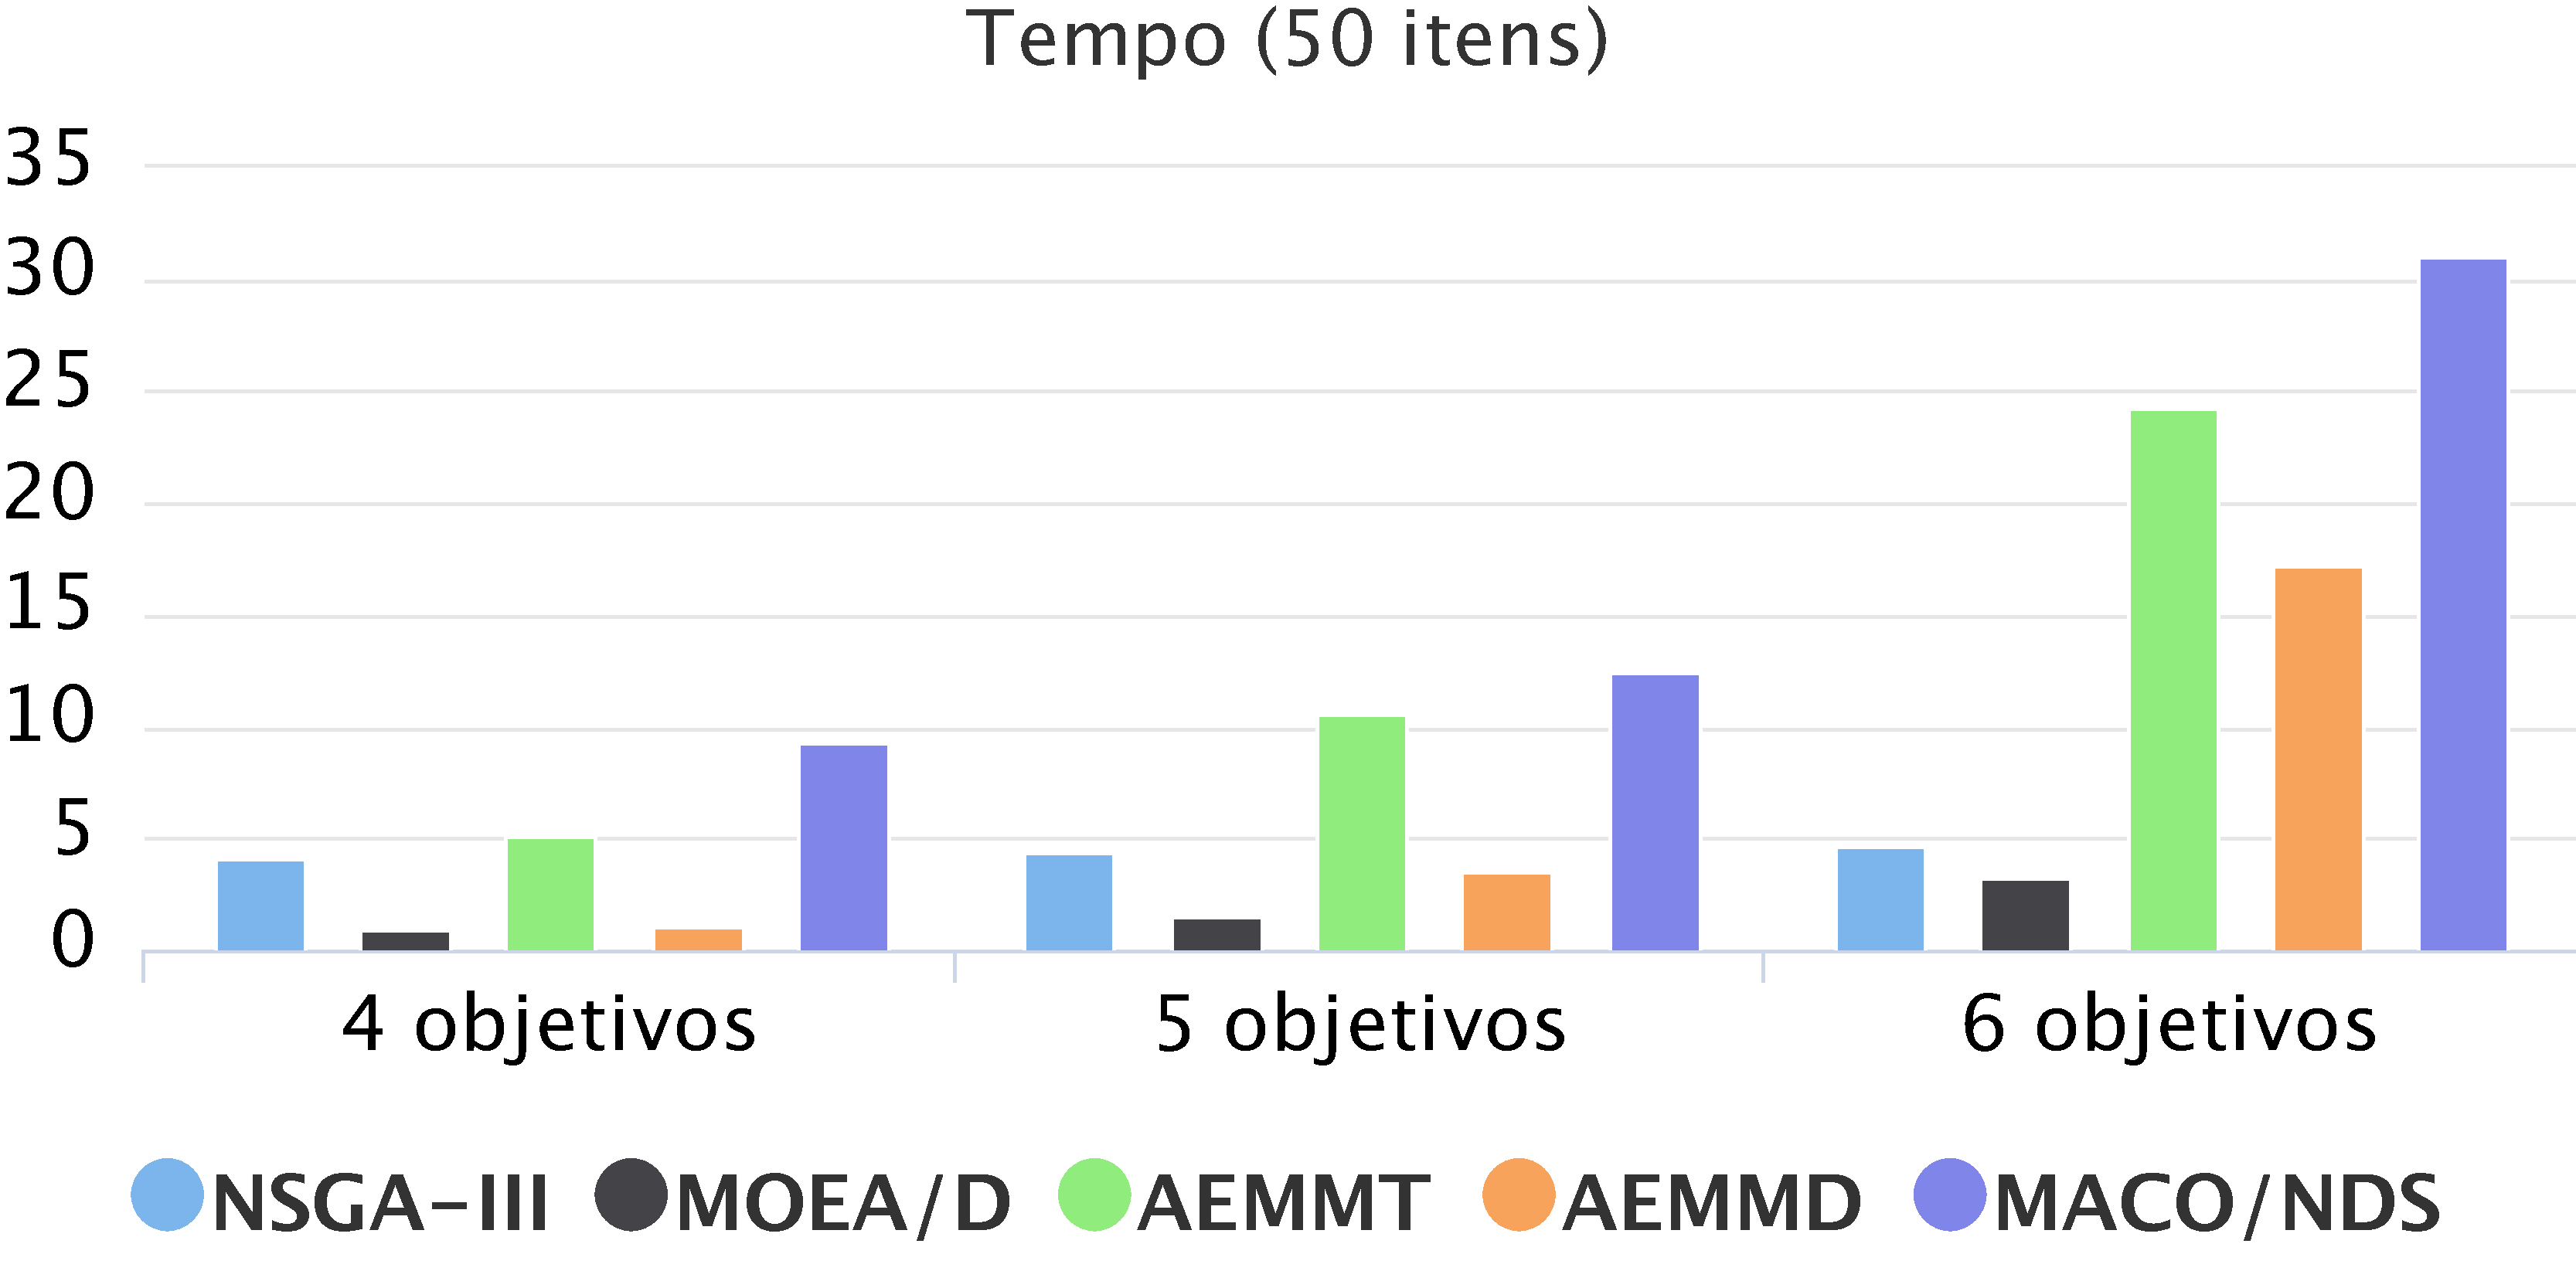
\includegraphics[width=0.5\textwidth]{cap_experimentos/figs/etapa3/time-mkp-50}
	\caption{\label{fig_exp3_pmm_50}Desempenho dos algoritmos na 3ª etapa para o PMM com 50 itens}
\end{figure*}

A \autoref{fig_exp3_pmm_50} mostra o desempenho dos algoritmos no PMM com 50 itens. Como pode ser observado, com exceção do GDp, as demais métricas apresentaram um comportamento similar ao das instâncias anteriores. O MACO/NDS e o AEMMT continuam sendo os algoritmos com menores taxas de erro. Enquanto o MACO/NDS consegue menor $ER$ em 4 e 5 objetivos, o AEMMT apresenta melhor resultado em 6 objetivos. O MACO/NDS obtém os melhores valores de $GDp$ e $PS$, e o MOEA/D é o algoritmo mais rápido. Dentre os algoritmos analisados, o MACO/NDS é o que apresenta o melhor compromisso entre as métricas e a melhor estabilidade quanto à qualidade de soluções (menor desvio padrão).

%!!todo!! Mudar o nome do MACO/NDS nas figuras
\begin{figure*}[!htbp]
	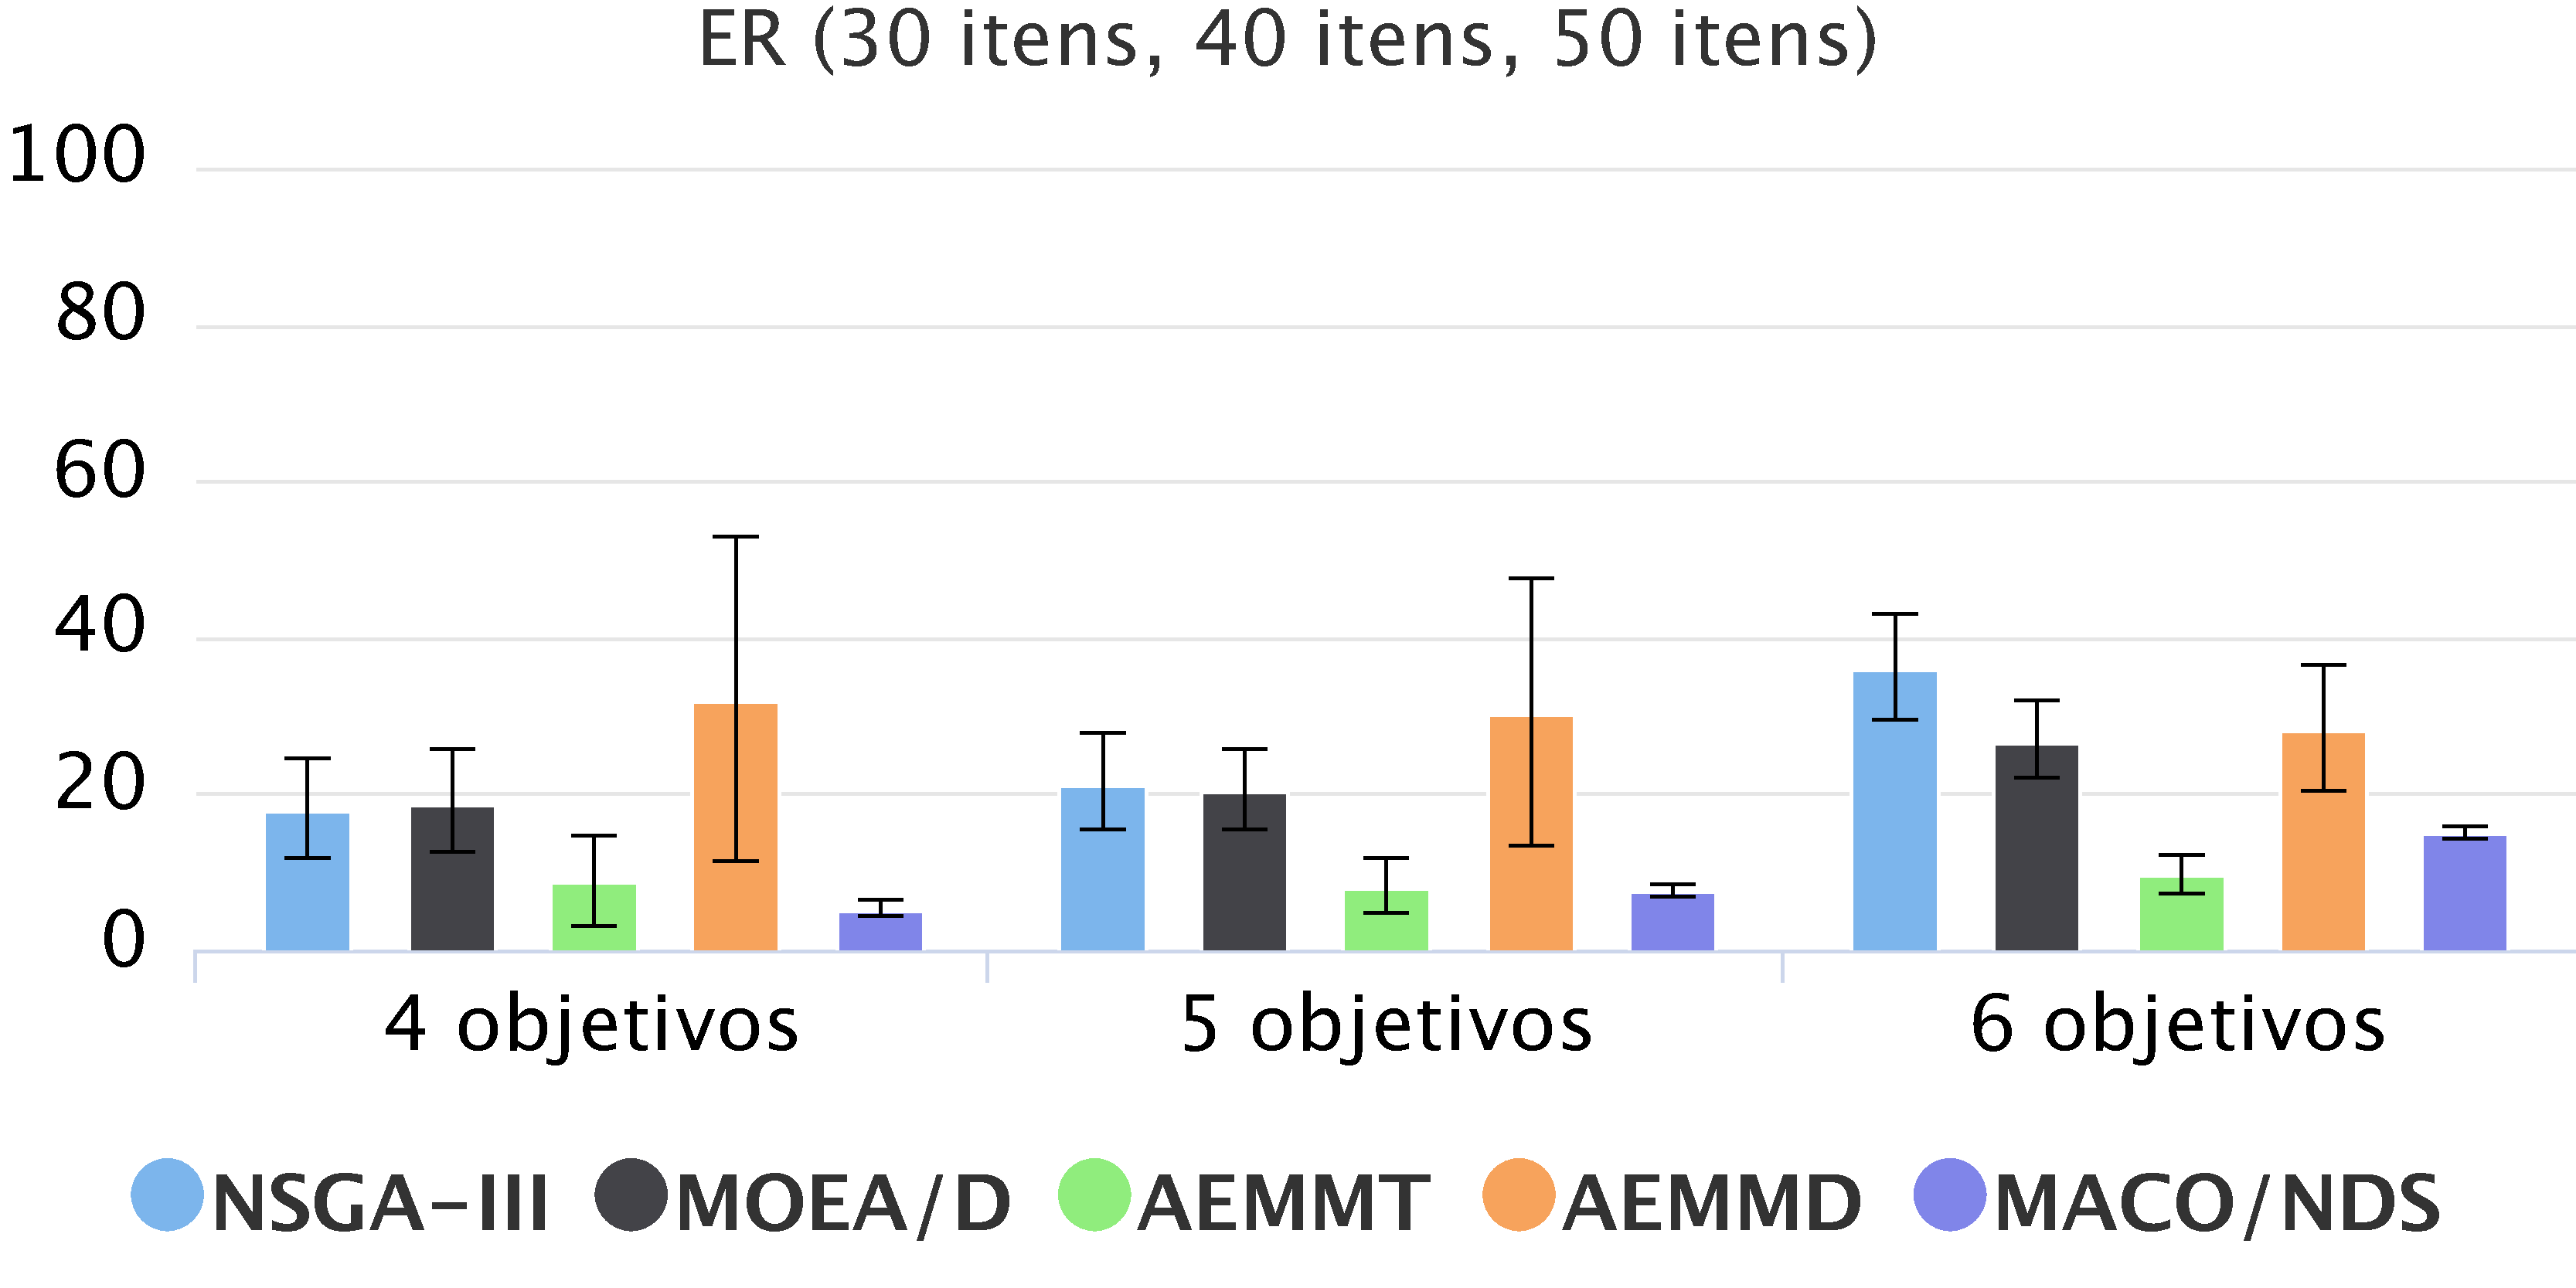
\includegraphics[width=0.5\textwidth]{cap_experimentos/figs/etapa3/er-mkp-todos}
	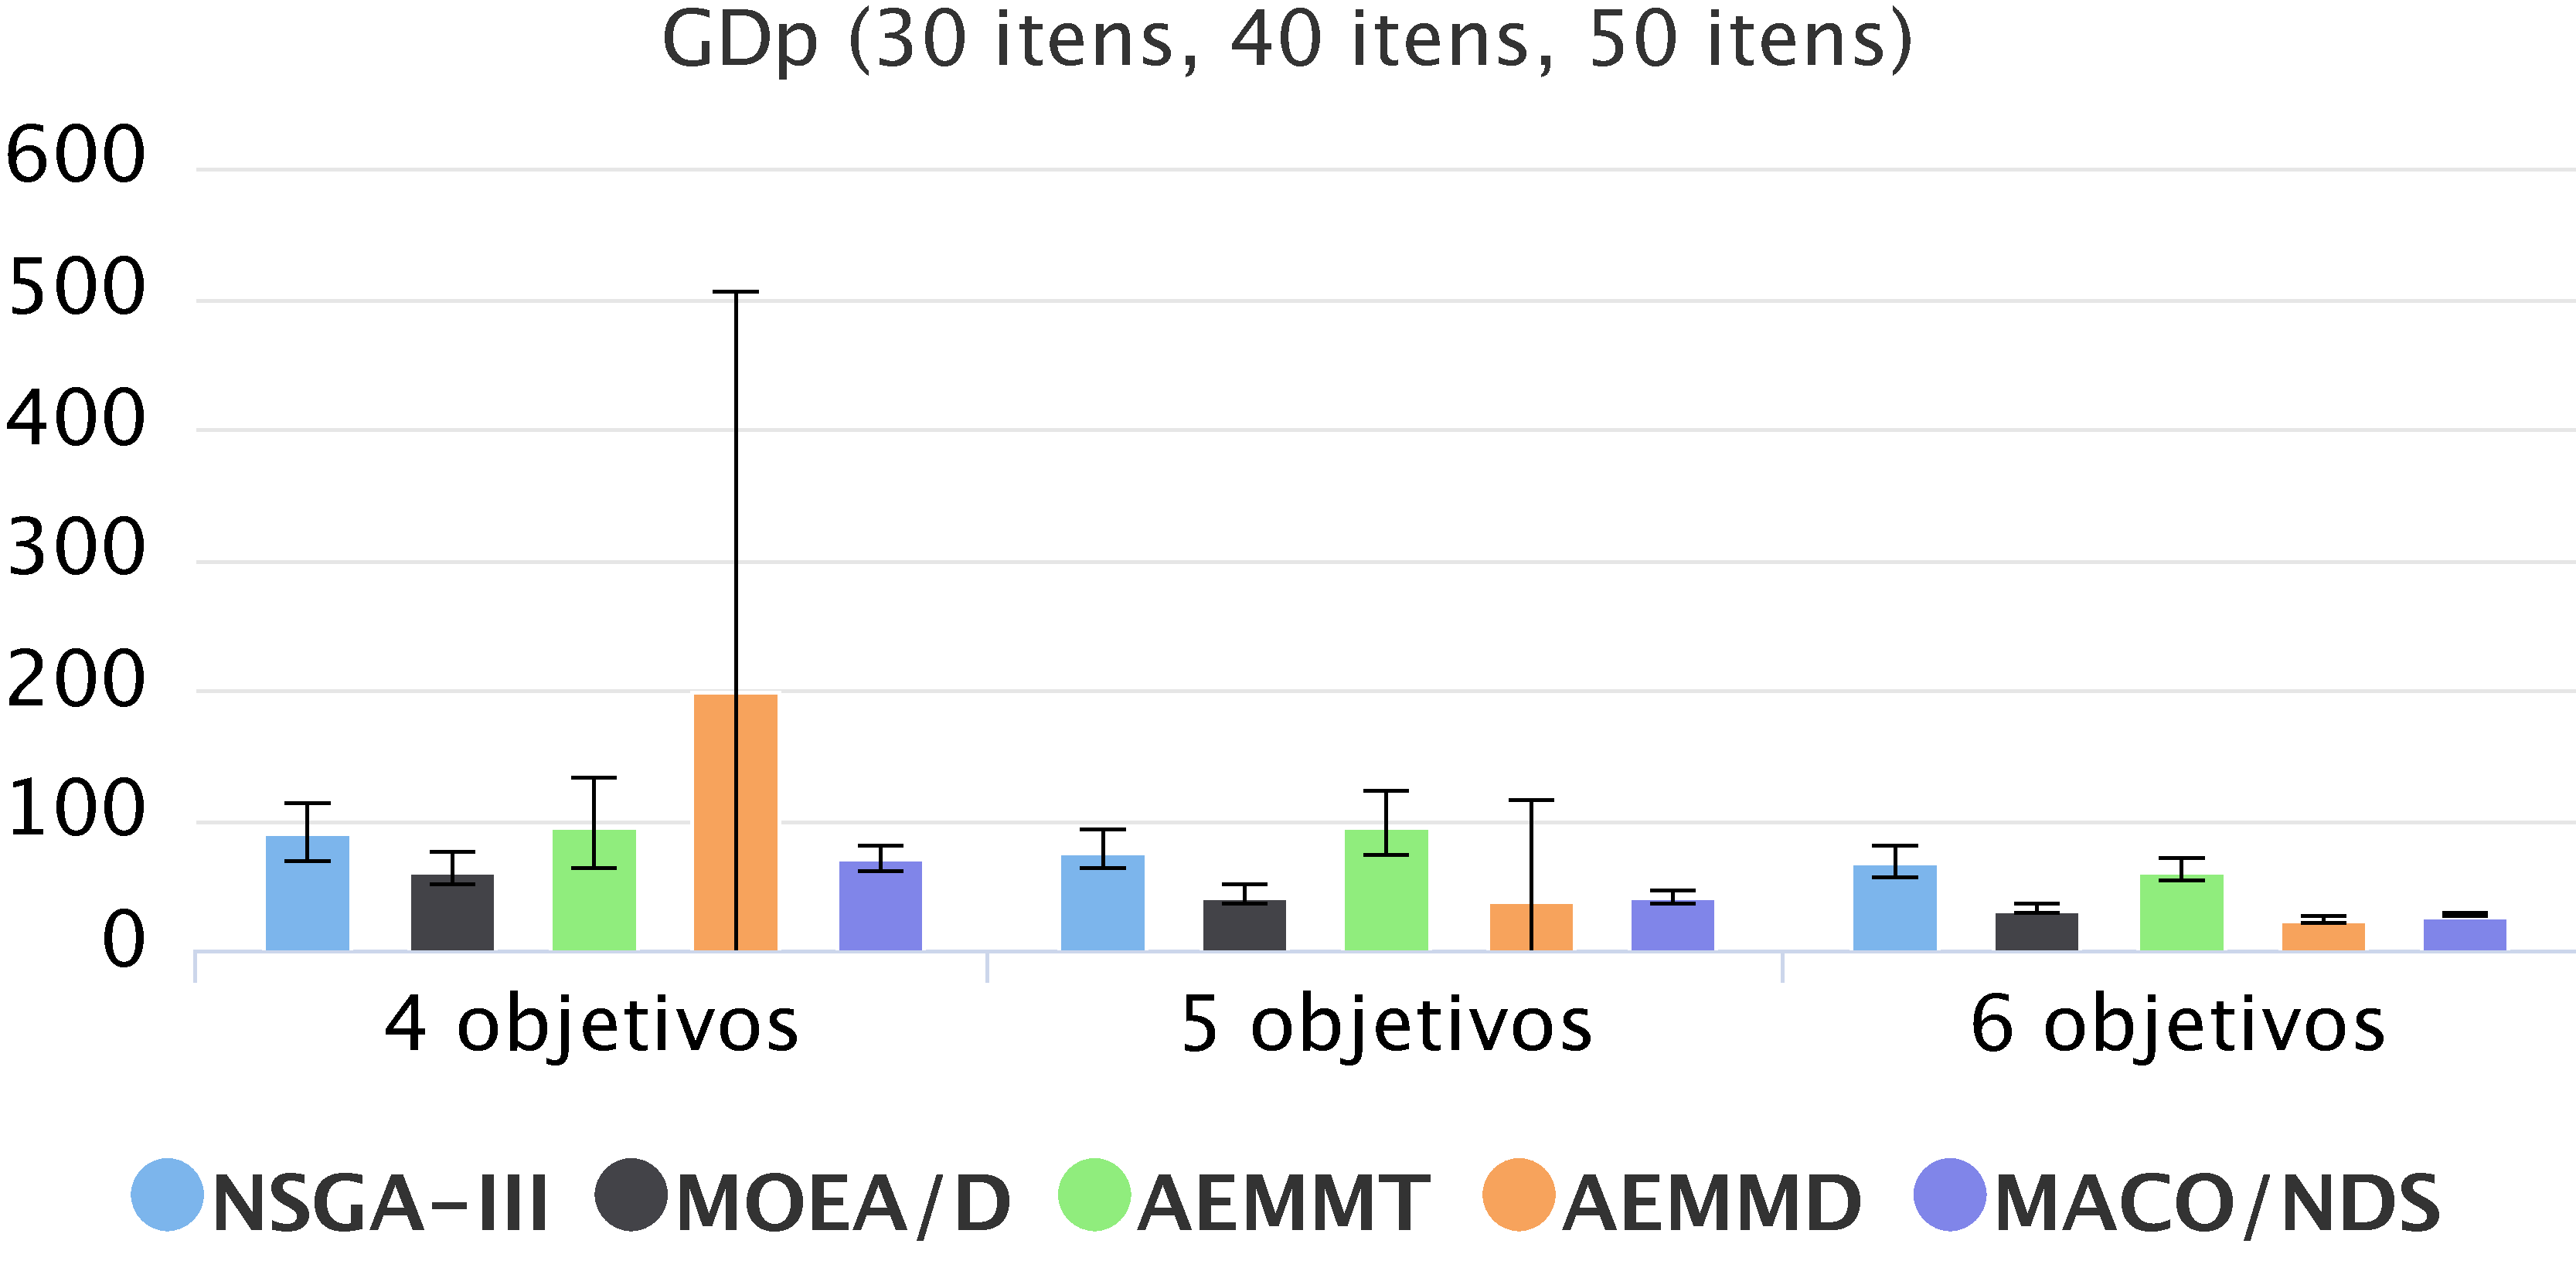
\includegraphics[width=0.5\textwidth]{cap_experimentos/figs/etapa3/gd-mkp-todos}
	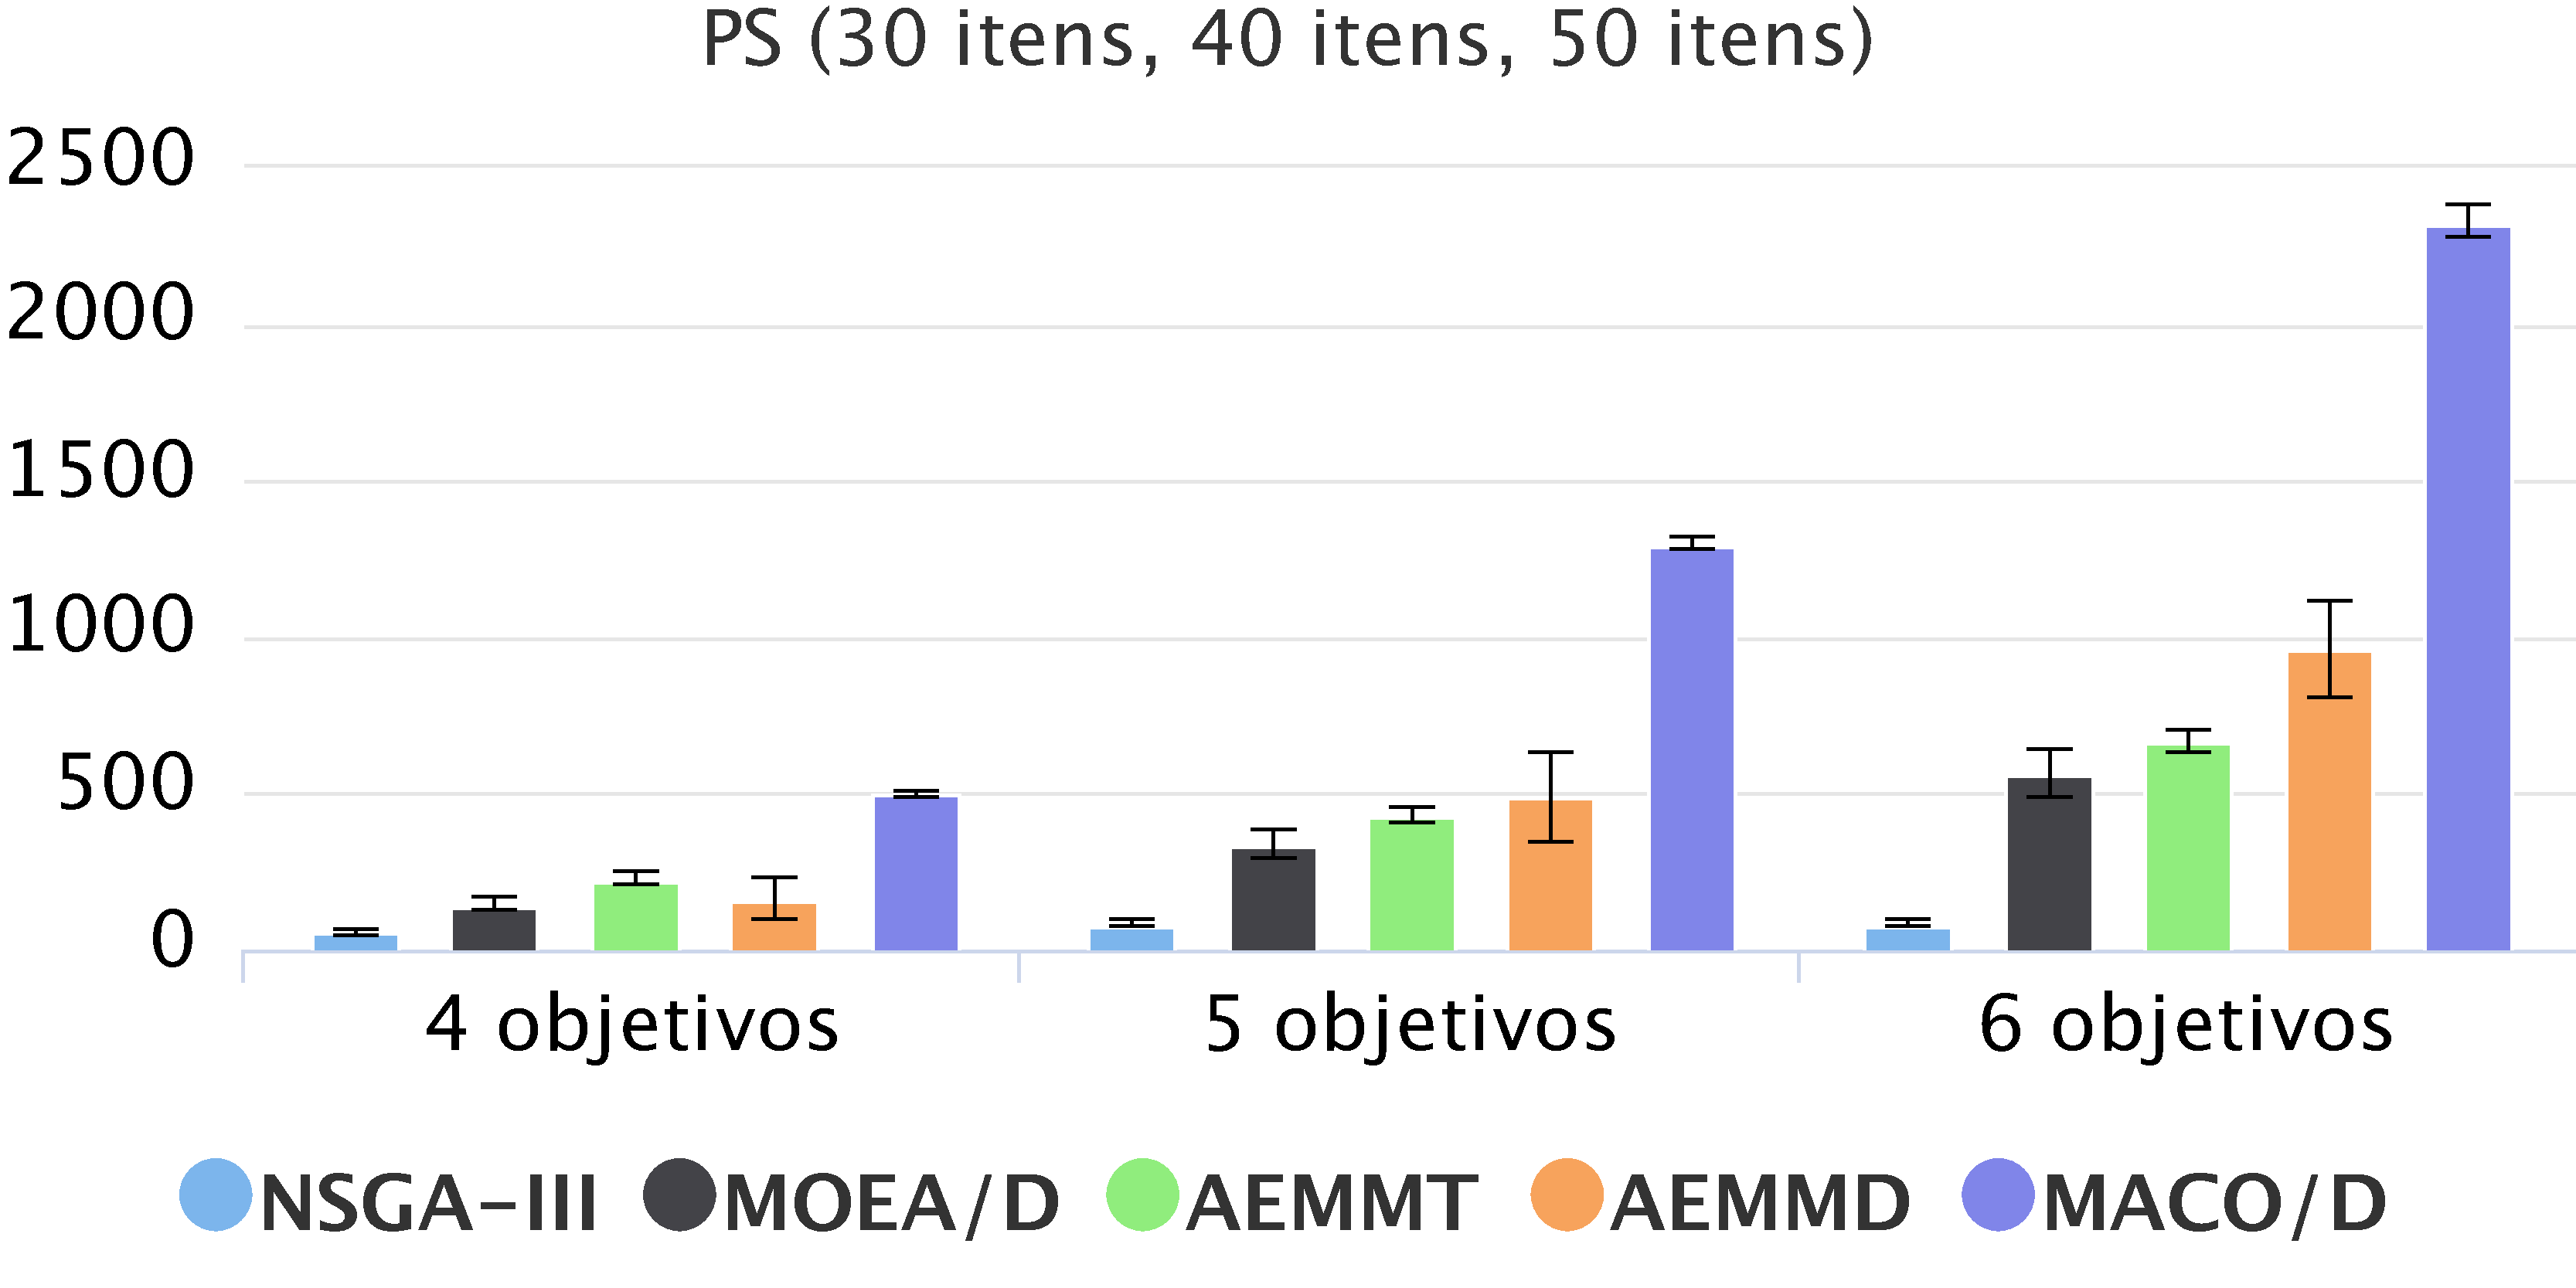
\includegraphics[width=0.5\textwidth]{cap_experimentos/figs/etapa3/ps-mkp-todos}
	\includegraphics[width=0.5\textwidth]{cap_experimentos/figs/etapa3/time-mkp-todos}
	\caption{\label{fig_exp3_pmm_todos}Resultado consolidado da 3ª etapa considerando o PMM com 30, 40 e 50 itens}
\end{figure*}

A fim de se fazer uma análise geral dos resultados, a média entre os 3 cenários é apresentada nos gráficos da \autoref{fig_exp3_pmm_todos}. As taxas de erro são muito baixas para o AEMMT e o MACO/NDS, quando comparados aos demais algoritmos. Os resultados em $GDp$ são bons para a maioria dos métodos. Apenas o AEMMD apresenta um valor alto de $GDp$ e com elevado desvio padrão para o problema de 4 objetivos (200 com desvio padrão de 504). O MOEA/D produz o melhor $GDp$ no problema de 4 objetivos (62,9), enquanto que, para 5 e 6 objetivos, o AEMMD (40,7 para 5 objetivos e 23,6 para 6) e o MACO/NDS (41,1 para 5 objetivos e 26,8 para 6) conseguem valores melhores que o MOEA/D (43 para 5 objetivos e 31,9 para 6), mas ainda similares. É importante notar que os desvios padrões no AEMMD são altos, representando uma certa instabilidade do algoritmo em gerar boas soluções. Em termos da cobertura da fronteira de Pareto ($PS$), o MACO/NDS alcançou os melhores valores em todas as formulações de objetivos. Analisando o tempo de execução médio, o AEMMT, o AEMMD e o MACO/S variam bastante com o número de objetivos, enquanto os demais são estáveis. O MOEA/D é o algoritmo mais rápido entre os avaliados nesta etapa dos experimentos.

\begin{figure*}[!htbp]
	\includegraphics[width=0.5\textwidth]{cap_experimentos/figs/etapa3/er-mrp-r1}
	\includegraphics[width=0.5\textwidth]{cap_experimentos/figs/etapa3/gd-mrp-r1}
	\includegraphics[width=0.5\textwidth]{cap_experimentos/figs/etapa3/ps-mrp-r1}
	\includegraphics[width=0.5\textwidth]{cap_experimentos/figs/etapa3/time-mrp-r1}
	\caption{\label{fig_exp3_prm_r1}Desempenho dos algoritmos na 3ª etapa para o PRM na rede 1}
\end{figure*}

Os gráficos correspondentes ao PRM na rede 1 são apresentados na \autoref{fig_exp3_prm_r1}. Em relação à taxa de erro, o AEMMD obtém os menores valores em todas as formulações de objetivos. Em seguida, aparecem o AEMMT e o MACO/NDS, respectivamente, mas com valores próximos. Por fim, os piores valores de ER foram obtidos pelo NSGA-III e pelo MOEA/D. Com relação ao $GDp$, é possível observar que o MACO/NDS e o MOEA/D atingem desempenhos bem próximos, sendo o MACO/NDS o melhor entre os dois. Considerando o tamanho das fronteiras de Pareto encontrada ($PS$), o AEMMD é o melhor algoritmo, seguido pelo MACO/NDS, AEMMT, MOEA/D e NSGA-III, nessa ordem. O MACO/NDS e o MOEA/D são os algoritmos mais rápidos e permanecem estáveis com o aumento do número de objetivos, enquanto o AEMMT e o AEMMD são os mais lentos e aumentam significativamente com o número de objetivos.

\begin{figure*}[!htbp]	
	\includegraphics[width=0.5\textwidth]{cap_experimentos/figs/etapa3/er-mrp-r2}
	\includegraphics[width=0.5\textwidth]{cap_experimentos/figs/etapa3/gd-mrp-r2}
	\includegraphics[width=0.5\textwidth]{cap_experimentos/figs/etapa3/ps-mrp-r2}
	\includegraphics[width=0.5\textwidth]{cap_experimentos/figs/etapa3/time-mrp-r2}
	\caption{\label{fig_exp3_prm_r2}Desempenho dos algoritmos na 3ª etapa para o PRM na rede 2}
\end{figure*}

A \autoref{fig_exp3_prm_r2} apresenta os resultados obtidos pelos algoritmos para a rede 2. Apesar de mais complexa, os gráficos apresentam um comportamento similar ao da instância anterior (rede 1). O AEMMD obtém as menores taxas de erro, seguido pelo AEMMT. Dentre as soluções incorretas encontradas, o MACO/NDS é o algoritmo que alcança os menores valores para a métrica $GDp$, sendo seguido de perto pelo AEMMT e pelo AEMMD. Considerando a métrica $PS$, os melhores valores foram encontrados pelo AEMMD, mas com uma diferença muito pequena em relação ao MACO/NDS. Os piores valores de $PS$ são retornados pelo NSGA-III. Tal comportamento é decorrência da limitação do algoritmo quanto ao crescimento do Pareto. Analisando o tempo médio de execução, o método mais rápido é o MOEA/D e o mais lento é o AEMMT.

\begin{figure*}[!htbp]
	\includegraphics[width=0.5\textwidth]{cap_experimentos/figs/etapa3/er-mrp-r3}
	\includegraphics[width=0.5\textwidth]{cap_experimentos/figs/etapa3/gd-mrp-r3}
	\includegraphics[width=0.5\textwidth]{cap_experimentos/figs/etapa3/ps-mrp-r3}
	\includegraphics[width=0.5\textwidth]{cap_experimentos/figs/etapa3/time-mrp-r3}
	\caption{\label{fig_exp3_prm_r3}Desempenho dos algoritmos na 3ª etapa para o PRM na rede 3}
\end{figure*}

A \autoref{fig_exp3_prm_r3} apresenta o desempenho dos algoritmos no PRM considerando a rede 3, o AEMMT encontra as melhores taxas de erro para 4 (15,2\%) e 5 (15,7\%) objetivos, enquanto que o MOEA/D consegue o melhor resultado para 6 objetivos (11,5\%). O NSGA-III produz o segundo menor $ER$ no problema de 4 objetivos (18,9\%), mas é o segundo pior para 5 objetivos (22,5\%) e o pior com 6 objetivos (52,7\%). O menor $GDp$ no problema com 4 objetivos é dado pelo MACO/NDS (0,7), enquanto o AEMMT obtém os melhores valores nos problemas com 5 e 6 objetivos (0,3 e 0,1, respectivamente). As maiores fronteiras de Pareto são encontradas pelo AEMMD e MACO/NDS, sendo o AEMMD o melhor entre os dois. O algoritmo mais rápido é o MACO/NDS, executando em tempo 5 vezes menor que o método mais lento (AEMMT).

\begin{figure*}[!htbp]	
	\includegraphics[width=0.5\textwidth]{cap_experimentos/figs/etapa3/er-mrp-todos}
	\includegraphics[width=0.5\textwidth]{cap_experimentos/figs/etapa3/gd-mrp-todos}
	\includegraphics[width=0.5\textwidth]{cap_experimentos/figs/etapa3/ps-mrp-todos}
	\includegraphics[width=0.5\textwidth]{cap_experimentos/figs/etapa3/time-mrp-todos}
	\caption{\label{fig_exp3_prm_todos}Resultado consolidado da 3ª etapa considerando o PRM nas redes 1, 2 e 3}
\end{figure*}

Para analisar de forma conjunta os resultados das três redes, todos os experimentos são consolidados através da média aritmética das métricas de desempenho avaliadas. Esses resultados consolidados são apresentados na \autoref{fig_exp3_prm_todos}. De maneira geral, o NSGA-III consegue soluções de qualidade razoável, mas apresenta baixo $PS$ e um tempo médio de execução mediano. O MOEA/D obtém as melhores taxas de erro no problema de seis objetivos, mas tem um desempenho modesto nos problemas de 4 e 5 objetivos. O algoritmo também está entre os piores para as métricas $GDp$ e $PS$. A velocidade de execução do MOEA/D é tão boa quanto a do MACO/NDS, sendo os dois algoritmos mais rápidos. Assim, o uso desse algoritmo pode ser uma boa opção quando o objetivo da busca é conseguir uma baixa taxa de erro em um curto tempo de execução, sem se preocupar com o $PS$. Analisando-se todas as métricas, os melhores resultados foram obtidos pelo AEMMD e o algoritmo proposto (MACO/NDS). Com relação ao erro, o AEMMD consegue as melhores taxas, enquanto o MACO/NDS, juntamente com o NSGA-III, apresentam os piores valores. Analisando-se o $GDp$, existe uma pequena diferença entre os algoritmos, mas o MACO/NDS gera melhores soluções que o AEMMD. Além disso, o desvio padrão do MACO/NDS é significativamente menor, tornando-o um método mais estável quanto à qualidade das soluções. Um desempenho similar também é observado para a métrica PS. Entretanto, nesse caso, o AEMMD produz as maiores fronteiras de Pareto que o MACO/NDS. Por outro lado, ao analisar o tempo médio de execução, observa-se que o MACO/NDS é consideravelmente mais rápido, chegando a executar em quase 5 vezes menos tempo. Considerando que o PRM é um problema sensível ao tempo de execução, apesar do AEMMD obter um desempenho razoavelmente superior nas métricas $ER$ e $PS$, o MACO/NDS é a melhor opção entre os algoritmos testados, pelo menos nos cenários analisados.

A principal diferença no desempenho do algoritmo proposto (MACO/NDS) em relação aos dois problemas investigados (PMM e PRM) é o tempo de execução. Considerando-se os resultados do PMM apresentados na \autoref{fig_exp3_pmm_todos}, o MACO/NDS é o segundo algoritmo mais lento e seu tempo de execução está altamente relacionado ao número de objetivos. Na \autoref{fig_exp3_prm_todos}, que representa o comportamento geral dos algoritmos no PRM, observa-se o oposto, ou seja, o MACO/NDS é o algoritmo mais rápido e seu tempo de execução se mantém estável, independentemente da formulação de objetivos. Concluímos que essa diferença de comportamento é decorrência do tamanho da fronteira de Pareto (soluções não dominadas). O processo de maior custo computacional no MACO/NDS é a atualização dos feromônios, onde é necessário recalcular o conjunto de soluções não-dominadas $nd$. A cada iteração, para toda solução criada, é necessário passar por todos elementos em $nd$ verificando a relação de não-dominância. Naturalmente, quanto maior o conjunto $nd$, mais caro se torna o processo. No PRM, foram encontradas fronteiras de Pareto de tamanho razoavelmente pequenos, todas com menos de 350 elementos. Nesse caso, para cada solução criada, é preciso fazer no máximo 350 comparações. No PMM, as fronteiras de Pareto são muito grandes. Por exemplo, no problema com 6 objetivos e 50 itens, a cardinalidade do conjunto $nd$ chega a ser maior que 4500 soluções. Quanto maior a quantidade de objetivos do problema, maior o número de soluções no Pareto e mais lento será a classificação de soluções não dominadas. Se o conjunto $nd$ é pequeno até mesmo para a maior quantidade de objetivos (caso do PRM), o processo será rápido e o tempo de execução não será muito diferente entre as formulações de objetivos. Por outro lado, se a cardinalidade de $nd$ é muito grande e cresce muito com o aumento da quantidade de objetivos, o tempo necessário para se atualizar os feromônios será muito alto e terá grande variação conforme a formulação de objetivos.

A fim de melhor comparar o MACO/NDS aos algoritmos AEMMT e AEMMD, realizou-se o teste de hipótese teste Z (\textit{Z-test}) com 5\% de significância ($\alpha=0,05$). Os resultados são mostrados nas Tabelas \ref{tab_ztest_meamt} e \ref{tab_ztest_meams}. Em ambas as tabelas, uma célula de fundo verde representa um cenário onde o MACO/NDS obteve melhor resultado que seu adversário, vermelho significa que o adversário foi melhor e a célula branca indica empate.

\begin{table}[htb]
	\centering
	\def\arraystretch{1.0}
	\caption{Testes de hipótese entre o MACO/NDS e o AEMMT para os problemas investigados}
	\label{tab_ztest_meamt}
	\begin{tabular}{cccccccccc}
		& \multicolumn{3}{l}{\textbf{4 objectives}} & \multicolumn{3}{l}{\textbf{5 objectives}} & \multicolumn{3}{l}{\textbf{6 objectives
		}} \\
		\textbf{Instance} & \textbf{ER} & \textbf{GDp} & \textbf{PS} & \textbf{ER} & \textbf{GDp} & \textbf{PS} & \textbf{ER} & \textbf{GDp} & \textbf{PS} \\ \hline
		30 items & \cellcolor{white} $=$ & \cellcolor{table-green} $<$ & \cellcolor{table-green} $>$ & \cellcolor{table-red} $>$ & \cellcolor{table-green} $<$ & \cellcolor{table-green} $>$ & \cellcolor{table-red} $>$ & \cellcolor{table-green} $<$ & \cellcolor{table-green} $>$ \\
		40 items & \cellcolor{table-green} $<$ & \cellcolor{table-green} $<$ & \cellcolor{table-green} $>$ & \cellcolor{table-green} $<$ & \cellcolor{table-green} $<$ & \cellcolor{table-green} $>$ & \cellcolor{table-red} $>$ & \cellcolor{table-green} $<$ & \cellcolor{table-green} $>$ \\
		50 items & \cellcolor{table-green} $<$ & \cellcolor{white} $=$ & \cellcolor{table-green} $>$ & \cellcolor{table-green} $<$ & \cellcolor{table-green} $<$ & \cellcolor{table-green} $>$ & \cellcolor{table-red} $>$ & \cellcolor{table-green} $<$ & \cellcolor{table-green} $>$ \\  \hline 
		Rede 1 & \cellcolor{table-red} $>$ & \cellcolor{table-green} $<$ & \cellcolor{table-red} $<$ & \cellcolor{table-red} $>$ & \cellcolor{table-green} $<$ & \cellcolor{table-green} $>$ & \cellcolor{table-red} $>$ & \cellcolor{table-green} $<$ & \cellcolor{table-green} $>$ \\
		Rede 2 & \cellcolor{table-red} $>$ & \cellcolor{table-green} $<$ & \cellcolor{table-green} $>$ & \cellcolor{table-red} $>$ & \cellcolor{table-green} $<$ & \cellcolor{table-green} $>$ & \cellcolor{table-green} $<$ & \cellcolor{table-green} $<$ & \cellcolor{table-green} $>$ \\
		Rede 3 & \cellcolor{table-red} $>$ & \cellcolor{table-green} $<$ & \cellcolor{table-red} $<$ & \cellcolor{table-red} $>$ & \cellcolor{table-green} $<$ & \cellcolor{table-green} $>$ & \cellcolor{table-red} $>$ & \cellcolor{table-red} $>$ & \cellcolor{table-green} $>$ \\  \hline 
	\end{tabular}
\end{table}

\begin{table}[htb]
	\centering
	\def\arraystretch{1.0}
	\caption{Testes de hipótese entre o MACO/NDS e o AEMMD para os problemas investigados}
	\label{tab_ztest_meams}
	\begin{tabular}{cccccccccc}
		& \multicolumn{3}{l}{\textbf{4 objectives}} & \multicolumn{3}{l}{\textbf{5 objectives}} & \multicolumn{3}{l}{\textbf{6 objectives
		}} \\
		\textbf{Instance} & \textbf{ER} & \textbf{GDp} & \textbf{PS} & \textbf{ER} & \textbf{GDp} & \textbf{PS} & \textbf{ER} & \textbf{GDp} & \textbf{PS} \\ \hline
		30 items & \cellcolor{table-green} $<$ & \cellcolor{table-green} $<$ & \cellcolor{table-green} $>$ & \cellcolor{table-green} $<$ & \cellcolor{table-red} $>$ & \cellcolor{table-green} $>$ & \cellcolor{table-green} $<$ & \cellcolor{table-red} $>$ & \cellcolor{table-green} $>$ \\
		40 items & \cellcolor{table-green} $<$ & \cellcolor{table-red} $>$ & \cellcolor{table-green} $>$ & \cellcolor{table-green} $<$ & \cellcolor{table-red} $>$ & \cellcolor{table-green} $>$ & \cellcolor{table-green} $<$ & \cellcolor{table-red} $>$ & \cellcolor{table-green} $>$ \\
		50 items & \cellcolor{table-green} $<$ & \cellcolor{table-green} $<$ & \cellcolor{table-green} $>$ & \cellcolor{table-green} $<$ & \cellcolor{table-green} $<$ & \cellcolor{table-green} $>$ & \cellcolor{table-green} $<$ & \cellcolor{table-green} $<$ & \cellcolor{table-green} $>$ \\  \hline 
		Rede 1 & \cellcolor{table-red} $>$ & \cellcolor{table-green} $<$ & \cellcolor{table-red} $<$ & \cellcolor{table-red} $>$ & \cellcolor{table-green} $<$ & \cellcolor{table-red} $<$ & \cellcolor{table-red} $>$ & \cellcolor{table-green} $<$ & \cellcolor{table-red} $<$ \\
		Rede 2 & \cellcolor{table-red} $>$ & \cellcolor{white} $=$ & \cellcolor{table-green} $>$ & \cellcolor{table-red} $>$ & \cellcolor{table-green} $<$ & \cellcolor{table-red} $<$ & \cellcolor{table-red} $>$ & \cellcolor{table-green} $<$ & \cellcolor{table-green} $>$ \\
		Rede 3 & \cellcolor{table-red} $>$ & \cellcolor{table-green} $<$ & \cellcolor{table-red} $<$ & \cellcolor{table-red} $>$ & \cellcolor{white} $=$ & \cellcolor{table-red} $<$ & \cellcolor{table-red} $>$ & \cellcolor{table-red} $>$ & \cellcolor{table-red} $<$ \\  \hline 
	\end{tabular}
\end{table}

Analisando-se o comportamento dos algoritmos, a partir da Tabela \ref{tab_ztest_meamt}, é possível confirmar a superioridade do MACO/NDS em relação ao AEMMT na maioria dos cenários, em ambos os problemas. Na comparação entre o MACO/NDS e o AEMMD, apresentados na Tabela \ref{tab_ztest_meams}, o algoritmo baseado em formigas foi melhor no PMM, mas pior no PRM. Entretanto, o teste de hipótese não considera o tempo de execução, no qual o MACO/NDS foi muito superior ao AEMMD, o que pode ser observado pela \autoref{fig_exp3_prm_todos}.

No PMM, se o tempo de execução é uma preocupação, a melhor alternativa é o algoritmo MOEA/D, que executa em tempo recorde e produz bons resultados. Se a rapidez do algoritmo não é tão importante e deseja-se encontrar um conjunto de soluções mais próximo do Pareto real, o MACO/NDS é o algoritmo mais indicado. No PRM, o método que representa melhor relação entre qualidade e tempo é o MACO/NDS. Por outro lado, se tempo não é importante, o AEMMD pode ser preferível.

A partir desses experimentos, foi elaborado e submetido um artigo científico que foi aceito e será publicado no \textit{2018 IEEE Congress on Evolutionary Computation} \cite{Franca2018}.

\section{Etapa 4: Análise baseada no hipervolume}
\label{section_experimentos_etapa4}

Na quarta etapa, os experimentos visam avaliar os algoritmos de otimização many-objective NSGA-III, SPEA2-SDE, MOEA/D, AEMMT, AEMMD, MOEA/D-ACO, MOACS e MACO/NDS em instâncias complexas do PMM e PRM utilizando a métrica hipervolume, a qual independe da estimação e/ou do conhecimento prévio da fronteira de Pareto. Esses experimentos são necessários, pois as etapas anteriores testaram apenas problemas com complexidade razoável, onde é possível estimar previamente a Fronteira de Pareto. Em grande parte dos problemas reais, esse conhecimento prévio é impraticável. Por exemplo, com a inclusão de mais itens no PMM ou o uso de redes mais complexas no PRM torna inviável a obtenção da fronteira de Pareto e se faz necessária a utilização de uma métrica não-paramétrica, neste caso o hipervolume, para avaliar o desempenho dos algoritmos. Nesses experimentos são utilizadas duas novas redes para o PRM, também investigadas em \cite{LafetaThesis}, e uma nova instância do PMM com 200 itens.

A fim de analisar o comportamento dos algoritmos em espaços de busca mais complexos, duas novas redes (redes 4 e 5) e duas novas instâncias do problema da mochila (100 e 200 itens) foram utilizadas. Entretanto, o aumento da complexidade influencia diretamente na cardinalidade do espaço de soluções, tornando inviável a obtenção de um conjunto estável de soluções não-dominadas (fronteira de Pareto aproximada). Tal situação é observada no PRM com as redes $R_3$, $R_4$ e $R_5$, e no PMM com 50, 100 e 200 itens. Nesses cenários, não é adequado basear as conclusões das análises em métricas de desempenho paramétricas, as quais são dependentes do Pareto aproximado. Por isso, nos experimentos dessa etapa, as avaliações consideram apenas duas métricas não-paramétricas, hipervolume e tempo, as quais são independentes do Pareto.

O hipervolume, junto ao \ac{IGD}, são as métricas mais utilizadas na literatura para avaliar algoritmos \textit{many-objective}. Uma definição do IGD pode ser encontrada em \cite{IGD}. Como explicado no início deste capítulo, o hipervolume calcula o volume da figura geométrica formada pelas distâncias das soluções encontradas a um ponto de referência pré-definido. Os pontos de referência utilizados nessa etapa para cada cenário avaliado são apresentados na Tabela \ref{table_exp4_pts_referencia}. Nessa tabela, os valores para o PMM são negativos, pois todos os algoritmos foram implementados para lidar com problemas de minimização. Dessa forma, como no problema da mochila deseja-se maximizar o valor de lucro carregado na mochila, todos os valores são multiplicados por -1 antes de se iniciar a busca.

\begin{table}[!htbp]
	\centering
	\caption{Pontos de referência e limitações no tamanho do arquivo usados para cada cenário de teste}
	\label{table_exp4_pts_referencia}
	\begin{tabular}{clll}
		\textbf{Instância}                                                       & \textbf{Obj.} & \textbf{Ponto de referência}                          & \textbf{Limite} \\ \hline
		\multirow{3}{*}{\begin{tabular}[c]{@{}c@{}}PMM\\ 50 itens\end{tabular}}  & 4             & {[}-15665; -17464; -19122; -16978{]}                   & 600             \\
		& 5             & {[}-15948; -15980; -14696; -14800; -14610{]}           & 1400            \\
		& 6             & {[}-16094; -14354; -12511; -14240; -17865; -11801{]}   & 4500            \\ \hline
		\multirow{3}{*}{\begin{tabular}[c]{@{}c@{}}PMM\\ 100 itens\end{tabular}} & 4             & {[}-30442; -25071; -30870; -29800{]}                   & 1300            \\
		& 5             & {[}-30673; -30266; -30171; -30922; -28821{]}           & 3200            \\
		& 6             & {[}-29389; -27406; -30824; -32040; -30531; -30171{]}   & 3400            \\ \hline
		\multirow{3}{*}{\begin{tabular}[c]{@{}c@{}}PMM\\ 200 itens\end{tabular}} & 4             & {[}-64608; -58090; -61540; -59399{]}                   & 1500            \\
		& 5             & {[}-62513; -63014; -58939; -64477; -65814{]}           & 3000            \\
		& 6             & {[}-59835; -60434; -65232; -60525; -60843; -60753{]}   & 3200            \\ \hline
		\multirow{3}{*}{\begin{tabular}[c]{@{}c@{}}PRM\\ Rede 3\end{tabular}}    & $P_4$         & {[}0,758449304; 283; 115; 52{]}                       & 90              \\
		& $P_5$         & {[}0,47215566; 0,776046738; 304; 159; 56{]}           & 250             \\
		& $P_6$         & {[}0,471416081; 0,776046738; 310; 159; 56; 83,459{]}  & 400             \\ \hline
		\multirow{3}{*}{\begin{tabular}[c]{@{}c@{}}PRM\\ Rede 4\end{tabular}}    & $P_4$         & {[}0,717830882; 185; 107; 33{]}                       & 90              \\
		& $P_5$         & {[}0,454221232; 0,776046738; 256; 157; 42{]}          & 200             \\
		& $P_6$         & {[}0,457194502; 0,776046738; 239; 157; 40; 80,667{]}  & 350             \\ \hline
		\multirow{3}{*}{\begin{tabular}[c]{@{}c@{}}PRM\\ Rede 5\end{tabular}}    & $P_4$         & {[}0,776046738; 259; 146; 43{]}                       & 90              \\
		& $P_5$         & {[}0,458729196; 0,776046738; 296; 166; 49{]}          & 100             \\
		& $P_6$         & {[}0,458729196; 0,776046738; 287; 177; 48; 101,938{]} & 250             \\ \hline
	\end{tabular}
\end{table}

Nesta etapa foram avaliados 8 algoritmos bio-inspirados \textit{many-objective}: NSGA-III, SPEA2-SDE, MOEA/D, AEMMT, AEMMD, MOEA/D-ACO, MOACS, e MACO/NDS. Esses algoritmos foram usados em 3 formulações de objetivo para cada problema (4, 5 e 6 objetivos) e 3 instâncias, totalizando 18 cenários de teste (problema, instância e objetivo). Foram realizadas 30 execuções, para cada algoritmo e em cada cenário, e os resultados foram calculados a partir das médias dos hipervolumes das execuções. O tempo foi avaliado através da média de três execuções em uma máquina i7-3770k@4.36GHz. Todos os algoritmos foram implementados na linguagem Javascript.

Os parâmetros utilizados na configuração de cada algoritmo podem ser encontrados na Tabela \ref{table_exp4_params}. Os parâmetros quantidade de formigas e tamanho dos grupos (marcados com ``*'' na tabela) dependem, respectivamente, das constantes $H$ e $K$ descritas originalmente em \cite{Ke2013}. Ambos os parâmetros $H$ e $K$ servem como guia para gerar os pesos aleatórios das formigas e dos grupos. Quanto maior o valor de $H$, maior será o número de formigas. A mesma relação também vale para $K$ e a quantidade de grupos. Em nossos experimentos foi adotado um mesmo valor para $K$ em todos os cenários testados (PMM e PRM). O valor de $H$ também foi constante para os cenários do PRM, mas variou de acordo com a quantidade de objetivos no PMM. No PMM, os valores de $H$ foram: $H=8$ para 4 objetivos, $H=6$ para 5 objetivos e $H=5$ para 6 objetivos. Independentemente dos valores adotados, o número de iterações no laço principal é ajustado para que sempre se tenha o mesmo número de avaliações (9000 no PRM e 15000 no PMM). Todos os parâmetros foram ajustados de acordo com execuções prévias dos algoritmos. 

\begin{table}[!htbp]
	\caption{Parâmetros utilizados pelos algoritmos da 4ª etapa, de acordo com o problema tratado.}
	\label{table_exp4_params}
	\begin{center}
		\begin{tabular}{c|r|r}
			\textbf{Parâmetro} & \textbf{PRM} &  \textbf{PMM} \\ %\hline
			\hline
			Tamanho da população               &    90 &      150 \\ %\hline
			Número de comparações        &   9000 &      15000 \\ %\hline
			Taxa de crossover                & 100\% &    100\% \\ %\hline
			Taxa de mutação                 &  20\% &      5\% \\ %\hline
			Tamanho da vizinhança (MOEA/D e MOEA/D-ACO)    &    10 &       10 \\ %\hline
			Tamanho das tabelas (MEAMT)   &    30 &       50 \\ %\hline
			Tamanho da tabela de dominância (MEAMT) &    90 &      150 \\ %\hline
			Número de divisões (NSGA-III)&     8 &        8 \\ %\hline
			$\alpha, \beta, \rho$ (ACOs)& 1; 2; 0,3 & 1; 4,3; 0,3 \\ %\hline
			Intervalo de valores para os feromônios (ACOs)& [0,1; 0,9] & [0,1; 0,9] \\ %\hline
			$\delta$ (MOEA/D-ACO)& 0,2 & 0,2 \\ %\hline
			$H$, relacionado à quantidade de formigas (MOEA/D-ACO)*& 6 & variável \\ %\hline
			$K$, relacionado à quantidade de grupos (MOEA/D-ACO)*& 3 & 3 \\ %\hline
			Taxa de elitismo (MOEA/D-ACO)& 0,9 & 0 \\ %\hline
			Tamanho das amostras (MACO/NDS)& 10 & 10 \\  %\hline
			Tamanho do grupo de estruturas ativas (MACO/NDS)& 5 & 5 \\
			\hline
		\end{tabular}
	\end{center}
\end{table}

Nesta etapa, a implementação dos algoritmos NSGA-III e SPEA2-SDE emprega uma estratégia diferente para limitar o tamanho do arquivo, ou seja, a fronteira de Pareto aproximada que é devolvida como solução da execução. Ao invés de impedir o crescimento do conjunto de soluções não-dominadas, além do tamanho máximo da população, esse limite foi ajustado para coincidir com o tamanho médio dos Paretos encontrados pelos algoritmos que retornaram os maiores conjuntos de soluções. Dessa forma, ambos algoritmos (NSGA-III e SPEA2-SDE) podem encontrar Paretos tão grandes quanto os demais métodos. A Tabela \ref{table_exp4_pts_referencia} mostra os limites utilizados para cada cenário de teste.

Para os algoritmos baseados em colônias de formigas (MOEA/D-ACO, MOACS e MACO/NDS), a fim de se testar o \textit{framework} da forma mais isolada possível, foi utilizada a mesma estratégia de construção da solução para os três métodos. O MOEA/D-ACO não foi proposto para os problemas da mochila nem do roteamento, o que fez necessária a adaptação da construção da solução em ambos os casos. O MOACS, por sua vez, já foi proposto para um problema parecido com o PRM, o problema do roteamento de veículos com janelas de tempo \cite{Baran2003}. Mesmo assim, preferiu-se utilizar o método proposto para o MACO/NDS, pois, através de experimentos prévios, observou-se que esse obteve melhore resultados no PRM. Essas estratégias de construção da solução para ambos os problemas estão descritas no capítulo \ref{chapter_macod}. No MOEA/D-ACO, cada formiga possui uma solução corrente que interfere nas probabilidades ao construir uma nova solução. Para suportar essa característica, o processo de construção foi adaptado de modo que, sempre, ao calcular o feromônio no MOEA/D-ACO, soma-se um novo termo correspondente à presença ou ausência da aresta (ou item) na solução atual da formiga.

Durante os experimentos, todas as 30 execuções para cada um dos 8 algoritmos foram realizadas para o PRM. Entretanto espaço de busca do problema da mochila é muito maior que o do roteamento \textit{multicast}, o que encarece muito o processo e o torna inviável em algumas situações. No PRM, o SPEA2-SDE foi, claramente, o algoritmo mais demorado. Entretanto no PMM, sua execução foi inviável. No cenário mais simples do problema, ou seja, 50 itens e 4 objetivos, o algoritmo levou 5,4 minutos para executar. Com 50 itens e 5 objetivos, o algoritmo precisou de 1 hora e 11 minutos. Já no próximo cenário, o computador apresentou problemas de memória. Por essa razão, o SPEA2-SDE não foi avaliado para o problema da mochila. Com relação ao NSGA-III, o tempo de execução foi muito superior aos demais algoritmos analisados para esse problema, chegando a mais de uma hora em uma das situações. Por essa razão, nos cenários com 6 objetivos, tomou-se a média de apenas 5 execuções ao invés das 30, originalmente previstas. Além disso, para facilitar a visualização do tempo de execução nos gráficos, excluiu-se essa informação referente ao NSGA-III Em vez disso, o tempo do NSGA-III, para cada um dos cenários do PMM, é informado na Tabela \ref{table_exp4_tempos_nsga3}). Assim, no PMM foram avaliados apenas 7 algoritmos, sendo que os cenários com 6 objetivos do NSGA-III foram feitos a partir da média de 5 execuções ao invés de 30.

\begin{table}[!htbp]
	\centering
	\caption{Tempos médios de execução para o NSGA-III nos cenários do PMM}
	\label{table_exp4_tempos_nsga3}
	\begin{tabular}{cll}
		\textbf{Instância}                                                       & \textbf{Obj.} & \textbf{Tempo de execução} \\ \hline
		\multirow{3}{*}{\begin{tabular}[c]{@{}c@{}}PMM\\ 50 itens\end{tabular}}  & 4             & 1m 1s                      \\
		& 5             & 5m 34s                     \\
		& 6             & 1h 9m 5s                   \\ \hline
		\multirow{3}{*}{\begin{tabular}[c]{@{}c@{}}PMM\\ 100 itens\end{tabular}} & 4             & 4m 39s                     \\
		& 5             & 30m 34s                    \\
		& 6             & 35m 10s                    \\ \hline
		\multirow{3}{*}{\begin{tabular}[c]{@{}c@{}}PMM\\ 200 itens\end{tabular}} & 4             & 6m 21s                     \\
		& 5             & 26m 52s                    \\
		& 6             & 30m 49s                    \\ \hline
	\end{tabular}
\end{table}

As Figuras \ref{fig_exp4_mkp_o4} a \ref{fig_exp4_mkp_o6} mostram o desempenho dos algoritmos nos 9 cenários do PMM, enquanto as Figuras \ref{fig_exp4_mrp_o4} a \ref{fig_exp4_mrp_o6} apresentam os gráficos com os resultados para os 9 cenários do PRM. O hipervolume é representado pelas barras e o eixo do lado esquerdo, enquanto o tempo de execução é mostrado pela linha e o eixo do lado direito. No eixo do hipervolume, as unidades $K$, $M$, $P$ e $E$ significam, respectivamente, $10^3$, $10^6$, $10^{15}$ e $10^{18}$. Em ambos os problemas, os gráficos foram agrupados por formulação de objetivo.

\begin{figure*}[!htbp]
	\includegraphics[width=1\textwidth]{cap_experimentos/figs/etapa4/i50o4}
	\includegraphics[width=1\textwidth]{cap_experimentos/figs/etapa4/i100o4}
	\includegraphics[width=1\textwidth]{cap_experimentos/figs/etapa4/i200o4}
	\caption{\label{fig_exp4_mkp_o4}Resultados dos algoritmos \textit{many-objective} no PMM com 4 objetivos}
\end{figure*}

Para 4 objetivos, o melhor valor de hipervolume é obtido pelo MOEA/D-ACO, seguido do MACO/NDS e do MOACS. Além disso, os dois algoritmos baseados em ACO com hipervolumes menores (MOACS e MACO/NDS) levam tempo similar ou maior que o MOEA/D-ACO. Portanto, o MOEA/D-ACO é o melhor ACO nesse cenário. Todos os algoritmos evolutivos obtêm valores de hipervolume muito abaixo àqueles obtidos pelos ACOs, mas o MOEA/D e o AEMMD têm a vantagem de serem muito mais rápidos, sendo que o MOEA/D apresenta a melhor relação custo/benefício, sendo a melhor opção entre os evolutivos.

\begin{figure*}[!htbp]
	\includegraphics[width=1\textwidth]{cap_experimentos/figs/etapa4/i50o5}
	\includegraphics[width=1\textwidth]{cap_experimentos/figs/etapa4/i100o5}
	\includegraphics[width=1\textwidth]{cap_experimentos/figs/etapa4/i200o5}
	\caption{\label{fig_exp4_mkp_o5}Resultados dos algoritmos \textit{many-objective} no PMM com 5 objetivos}
\end{figure*}

Os resultados para 5 objetivos não mudam muito em relação à formulação anterior. O MOEA/D-ACO continua sendo o algoritmo que obtém o melhor valor de hipervolume. Dentre os três algoritmos baseados em colônia de formiga, o MOACS apresentou o pior resultado, tanto em tempo quanto em hipervolume. O MACO/NDS executou em tempo similar ao melhor algoritmo (MOEA/D-ACO), mas obteve pior desempenho em relação ao hipervolume. Novamente, os algoritmos evolutivos atingiram hipervolumes inferiores aos ACOs, com exceção do NSGA-III, que apesar do alto custo em tempo de execução, conseguiu um valor de hipervolume similar ao MOACS. Em termos de tempo de execução, o melhor algoritmo foi o MOEA/D, mas seu hipervolume foi muito baixo em comparação aos métodos com os melhores resultados.

\begin{figure*}[!htbp]
	\includegraphics[width=1\textwidth]{cap_experimentos/figs/etapa4/i50o6}
	\includegraphics[width=1\textwidth]{cap_experimentos/figs/etapa4/i100o6}
	\includegraphics[width=1\textwidth]{cap_experimentos/figs/etapa4/i200o6}
	\caption{\label{fig_exp4_mkp_o6}Resultados dos algoritmos \textit{many-objective} no PMM com 6 objetivos}
\end{figure*}

Com 6 objetivos, o tempo médio necessário para executar os algoritmos AEMMT e AEMMD saltam, tornando-os ainda menos eficientes para o PMM. Nesses cenários, o MOEA/D-ACO possui, em geral, o segundo menor tempo de execução, perdendo apenas para o MOEA/D. O melhor hipervolume, assim como nas formulações de objetivo anteriores, é dado pelo MOEA/D-ACO, o que faz dele o melhor algoritmo, pois consegue o melhor conjunto de soluções em um tempo satisfatório.

Em geral, no problema da mochila, todos os métodos evolutivos obtiveram hipervolumes baixos quando comparados aos ACOs. Em termos de tempo médio de execução, o MOEA/D é, de longe, o algoritmo mais rápido dentre todos os métodos investigados. O NSGA-III, apesar de conseguir o melhor hipervolume dentre os algoritmos evolutivos, é muito mais lento que qualquer outro método. Além disso, apresenta valores de hipervolume menores que as abordagens baseadas em ACO. Portanto, não é uma boa opção em nenhum dos cenários analisados. Demandando um maior tempo de execução, mas ainda se mantendo abaixo de 1 minuto, o MOEA/D-ACO e o MACO/NDS geram conjuntos de soluções de qualidade muito superior aos obtidos pelos algoritmos evolutivos. Dentre os três ACOs, o MOACS demorou mais a executar e obteve os piores resultados, enquanto o MOEA/D-ACO foi superior tanto em hipervolume quanto em tempo, fazendo dele o melhor algoritmo para o problema da mochila multiobjetivo considerando-se os cenários analisados.

\begin{figure*}[!htbp]	
	\includegraphics[width=1\textwidth]{cap_experimentos/figs/etapa4/r3o4}
	\includegraphics[width=1\textwidth]{cap_experimentos/figs/etapa4/r4o4}
	\includegraphics[width=1\textwidth]{cap_experimentos/figs/etapa4/r5o4}
	\caption{\label{fig_exp4_mrp_o4}Resultados dos algoritmos \textit{many-objective} no PRM com 4 objetivos}
\end{figure*}

No PRM, o primeiro gráfico da \autoref{fig_exp4_mrp_o4} mostra o desempenho dos algoritmos quando submetidos ao cenário mais simples (rede 3 com 4 objetivos). Nesse cenário, o AEMMD apresenta o pior hipervolume (922), enquanto o MOACS e o MACO/NDS se destacam, sendo o MOACS o melhor, tanto em hipervolume quanto em tempo de execução (2548 em 8,2 segundos). Os algoritmos evolutivos SPEA2-SDE e o AEMMT atingem um hipervolume próximo ao do o MACO/NDS, mas levam consideravelmente mais tempo para executar (2207 em 15,1 segundos e 2141 em 15,5 segundos, respectivamente). Neste cenário, o MOACS é claramente a melhor estratégia para o problema.

Na rede 4 com 4 objetivos (segundo gráfico da \autoref{fig_exp4_mrp_o4}), os algoritmos evolutivos apresentaram os hipervolumes mais baixos, enquanto que as abordagens baseadas em colônias de formigas retornaram os maiores valores. O MOEA/D-ACO é o algoritmo mais rápido e obtém um bom hipervolume (7502 em 4,3 segundos), enquanto o MOACS resultou no melhor hipervolume, mas gastando um pouco mais de tempo (8330 em 7,1 segundos). O MACO/NDS foi o pior algoritmo baseado em formiga para esse cenário, apesar do desempenho muito superior aos AEMOs. Ele precisa de 9,5 segundos de execução para atingir um hipervolume de 5953.

A rede 5 é a mais complexa utilizada em nossos experimentos. Considerando os resultados dos experimentos com 4 objetivos, apresentados no terceiro gráfico da \autoref{fig_exp4_mrp_o4}, o NSGA-III apresentou o pior resultado de hipervolume (1036). O MOEA/D-ACO levou praticamente o mesmo tempo que o algoritmo MOEA/D (6,3 contra 6,5 segundos), mas obteve um hipervolume consideravelmente maior (5904 contra 4292). Já os demais algoritmos evolutivos (SPEA2-SDE, AEMMD e AEMMT), atingiram um desempenho intermediário (4985, 4756 e 5305, respectivamente). Os melhores valores de hipervolume foram obtidos pelo MACO/NDS e pelo MOACS. Entretanto, a melhor relação custo/benefício foi obtida pelo MOACS, que apresentou o segundo maior hipervolume (5904) e um tempo de execução razoável (9,5 segundos). O MACO/NDS, apesar de alcançar o melhor valor de hipervolume (5927), teve o pior desempenho em tempo de execução (13,4 segundos).

\begin{figure*}[!htbp]	
	\includegraphics[width=1\textwidth]{cap_experimentos/figs/etapa4/r3o5}
	\includegraphics[width=1\textwidth]{cap_experimentos/figs/etapa4/r4o5}
	\includegraphics[width=1\textwidth]{cap_experimentos/figs/etapa4/r5o5}
	\caption{\label{fig_exp4_mrp_o5}Resultados dos algoritmos \textit{many-objective} no PRM com 5 objetivos}
\end{figure*}

Para a rede 3 com 5 objetivos (primeiro gráfico da \autoref{fig_exp4_mrp_o5}), o SPEA2 com a modificação SDE resultou no melhor hipervolume entre todos os algoritmos (66.647). Em contrapartida, o custo do algoritmo, uma das principais desvantagens do SPEA2, também é um problema para o SPEA2-SDE. Nos experimentos, a execução desse algoritmo exigiu um tempo muito maior que as demais estratégias. Enquanto a execução do SPEA2-SDE demora, em média, 1,71 minutos, o NSGA-III (segundo pior algoritmo em tempo) demanda 42,1 segundos e as abordagens baseadas em ACO gastam, em média, 5,2 segundos. Em termos de hipervolume, os piores resultados foram obtidos pelos algoritmos AEMMT, NSGA-III, MOEA/D e MOEA/D-ACO, nesta ordem. O AEMMD também apresentou bom valor de hipervolume (65.747), bem próximo do SPEA2-SDE, só que com um tempo de execução bem mais baixo (17 segundos). Os algoritmos MOACS e MACO/NDS são mais rápidos (6,7 e 7,8 segundos, respectivamente) e atingiram bons valores de hipervolume (44.303 e 46.033), embora inferiores ao AEMMD. Neste cenário, não está claro qual é o melhor algoritmo. Se o hipervolume for priorizado em relação ao tempo de execução, o AEMMD é a melhor opção. Caso seja aceitável uma pequena redução no desempenho em favor de um algoritmo mais rápido, tanto o MOACS quanto o MACO/NDS são adequados. Ainda, se for analisada a relação hipervolume/tempo, tem-se que o melhor algoritmo é o MOACS (6612 $HV/s$), seguido do MACO/NDS (5902 $HV/s$) e do AEMMD (3867 $HV/s$).

Considerando o segundo gráfico da \autoref{fig_exp4_mrp_o5} (rede 4 com 5 objetivos), o SPEA2-SDE volta a mostrar os melhores valores para o hipervolume (122.749). Entretanto, seu alto custo (42,9 segundos) em relação aos demais algoritmos, o torna menos atrativo em aplicações práticas. Os algoritmos AEMMD e MOACS são os que apresentam melhor desempenho geral. Enquanto o AEMMD consegue o segundo maior hipervolume (94.005) e leva 10 segundos para executar, o MOACS atinge um hipervolume um pouco mais baixo (87.681) em 7,3 segundos. Os algoritmos MACO/NDS e MOEA/D apresentam um desempenho similar e um pouco abaixo dos algoritmos anteriores. O MACO/NDS obteve um hipervolume de 75.276 em 8,3 segundos de execução, enquanto que o MOEA/D atingiu 65.579 de hipervolume em 6,3 segundos. Os piores valores de hipervolume foram retornados pelo NSGA-III e AEMMT (6.554 e 45.310, respectivamente).

Na rede 5 com 5 objetivos (terceiro gráfico da \autoref{fig_exp4_mrp_o5}), os melhores hipervolumes são dados pelo AEMMD e MACO/NDS. O AEMMD apresenta um conjunto de soluções de melhor qualidade (47.297 de hipervolume), mas leva um pouco mais de tempo para calculá-las (12,7 segundos). As soluções encontradas pelo MACO/NDS são ligeiramente inferiores (43.666 de hipervolume), mas o tempo necessário para obtê-las é um pouco menor (11 segundos).

\begin{figure*}[!htbp]	
	\includegraphics[width=1\textwidth]{cap_experimentos/figs/etapa4/r3o6}
	\includegraphics[width=1\textwidth]{cap_experimentos/figs/etapa4/r4o6}
	\includegraphics[width=1\textwidth]{cap_experimentos/figs/etapa4/r5o6}
	\caption{\label{fig_exp4_mrp_o6}Resultados dos algoritmos \textit{many-objective} no PRM com 6 objetivos}
\end{figure*}

No primeiro gráfico da \autoref{fig_exp4_mrp_o6}, que mostra os resultados para a rede 3 com 6 objetivos, o SPEA2-SDE repete o comportamento dos cenários anteriores, ou seja, consegue um resultado de hipervolume muito bom, mas a um custo muito alto de tempo (4.768.243 em 6,53 minutos). O MOACS retorna um ótimo valor de hipervolume a um custo muito pequeno em tempo (4.162.784 em 7,3 segundos). O AEMMD consegue hipervolume pouco melhor que o MOACS (4.394.789), mas exigindo quase o quádruplo ($3,6\times$) do tempo de execução (26,6 segundos). O MACO/NDS obteve um valor intermediário para o hipervolume (2.538.591), com um tempo de execução similar ao MOACS (8,4 segundos). Os demais algoritmos, apesar de terem um bom tempo de execução (exceto o NSGA-III), retornaram valores muito baixos para o hipervolume. 

Na rede 4 com 6 objetivos (segundo gráfico da \autoref{fig_exp4_mrp_o6}), o melhor hipervolume é dado pelo MACO/NDS (8.684.287), seguido de perto pelo SPEA2-SDE (8.073.724), pelo MOACS (7.816.354) e pelo AEMMD (7.329.717). Devido ao seu tempo de execução (3 minutos), o SPEA-SDE possui uma péssima relação custo/benefício quando comparado às demais abordagens. O AEMMD possui um tempo de execução satisfatório, mas pior que as abordagens baseadas em ACO. Entre o MOACS e o MACO/NDS, o segundo consegue um conjunto de soluções de qualidade superior ao primeiro e leva apenas um segundo a mais para executar, sendo o algoritmo indicado para esse cenário.

O terceiro gráfico da \autoref{fig_exp4_mrp_o6} apresenta os resultados obtidos para o cenário mais complexo do PRM nesta etapa, o qual é dado pela rede 5 com 6 objetivos. Nele, os piores resultados foram encontrados pelo NSGA-III (53.130) e MOEA/D-ACO (743.365) e MOEA/D (2.385.997). O SPEA2-SDE e o AEMMT obtiveram valores intermediários de hipervolumes (4.731.148 e 3.954.286, respectivamente), mas , junto com o NSGA-III, apresentam os piores tempos de execução: 6,26 minutos para o SPEA2-SDE, 34,1 segundos para o NSGA-III e 26,8 segundos para o AEMMT. Novamente, repetindo o ocorrido no cenário anterior, o AEMMD e MACO/NDS foram os algoritmos que atingiram os melhores resultados de hipervolume. O AEMMD com hipervolume melhor e tempo pior (7.577.440 em 21,7 segundos), e o MACO/NDS com hipervolume pior e tempo melhor (7.402.986 em 11,2 segundos).

De forma geral, percebe-se que o SPEA2-SDE encontra ótimos resultados, mas a um custo muito alto de tempo de execução, tornando-o inviável para aplicações como o PRM, onde é importante que se tenha uma resposta rápida sobre qual rota tomar. Dentre os métodos evolutivos, o melhor método foi o AEMMD que, na maioria dos casos, conseguiu um bom hipervolume com um tempo de execução satisfatório. A grande vantagem das abordagens baseadas em ACO em relação aos algoritmos evolutivos investigados está no tempo de execução. Além disso, em 4 dos 9 cenários testados, os algoritmos baseados em formigas ultrapassam os AGs também em hipervolume. Para o PRM, parece ser mais adequado utilizar uma abordagem baseada em ACO, pois assim é possível encontrar soluções de ótima qualidade a um custo computacional menor. Dentre os três ACOs investigados, na maioria da vezes, o MOACS apresentou melhores resultados que o MACO/NDS, tanto em tempo quanto em hipervolume. Entretanto, é importante notar notar que, na rede 5, os valores de hipervolume alcançados pelo MACO/NDS superam os do MOACS em todas as formulações de objetivos. Isso é um indício que o MACO/NDS pode se tornar a melhor alternativa para redes mais complexas. Também é importante destacar que o MOACS implementado neste trabalho utiliza a abordagem do MACO/NDS para construir as soluções. Através de experimentos preliminares, foi possível observar que essa modificação melhorou o desempenho do algoritmo em relação à sua versão original \cite{Riveros2016}.

Considerando ambos os problemas, tanto o NSGA-III quanto o SPEA2-SDE não obtiveram desempenho satisfatório. O NSGA-III é muito caro computacionalmente para o PMM e não produz resultados muito bons de hipervolume no PRM. O SPEA2-SDE leva muito tempo para executar tanto no PMM como no PRM, sendo inviável em ambos. O MOEA/D gera bons resultados em alguns cenários específicos do PRM, como a rede 5 com 4 e a rede 5 com 5 objetivos, mas, em geral, apesar de apresentar bons valores de tempo de execução, não atinge um hipervolume satisfatório. Os algoritmos AEMMT e AEMMD têm desempenho muito ruim no PMM, mas, em contrapartida, atingem bons valores de hipervolume no PRM, sendo que o AEMMD consegue o melhor resultado em vários cenários (rede 5 com 5 objetivos e rede 5 com 6 objetivos, por exemplo). A deficiência do AEMMT e do AEMMD está no tempo de execução, que é, em geral, superior aos algoritmos baseados em colônia de formigas. Os resultados mais interessantes foram obtidos pelos ACOs, que conseguiram bons valores de hipervolumes a custos razoáveis de tempo. No PMM, o melhor algoritmo foi o MOEA/D-ACO, com valores de hiper-volume muito superiores aos AGs e tempo de execução, apesar de maior que os algoritmos evolutivos (excluindo o NSGA-III), inferior a 1 minuto. No PRM, os melhores algoritmos foram o AEMMD, o MOACS e o MACO/NDS. Em geral, o AEMMD obteve melhores valores de hipervolume, mas a um custo maior de tempo, enquanto os ACOs conseguiram valores muito bons de hipervolume a um custo menor de tempo. Entre o MOACS e MACO/NDS, o primeiro atingiu melhor hipervolume e tempo médio de execução na maioria dos cenários, mas o MACO/NDS conseguiu os melhores resultados nos testes mais complexos (redes 4 e 5 com 6 objetivos), o que é um indício de que possa funcionar melhor em instâncias mais complexas do problema. Também é interessante notar que o MACO/NDS foi o único algoritmo a conseguir bom desempenho tanto no problema da mochila quanto no problema do roteamento. De forma geral, considerando-se os 8 algoritmos investigados, o MACO/NDS foi o algoritmo de comportamento mais estável ao ser avaliado sobre os dois problemas discretos.


% ---
% Finaliza a parte no bookmark do PDF, para que se inicie o bookmark na raiz
% ---
\bookmarksetup{startatroot}% 
% ---

% ---
% Conclusão
% ---
\chapter[Conclusão]{Conclusão}
Este trabalho estendeu a pesquisa de \cite{Bueno2010} e \cite{Lafeta2016}, adicionando um novo problema de teste, o problema da mochila multiobjetivo (PMM), e 6 novos algoritmos many-objectives, sendo 3 deles AG's (MOEA/D, SPEA2-SDE e NSGA-III) e 3 deles ACO's (MOACS, MOEA/D-ACO e MACO/D). Dentre os ACO's incluídos no trabalho, um deles, o \textit{Many-objective Ant Colony Optimization based on Decomposed Pheromone} (MACO/D), foi proposto pelo autor juntamente com uma nova estratégia de construção de solução para o problema do roteamento multicast (PRM).

O primeiro objetivo do trabalho, representado pela etapa 1 de experimentos (seção \ref{section_experimentos_etapa1}), foi incluir o novo problema PMM e comparar os algoritmos NSGA-II, SPEA2, MOEA/D, NSGA-III e AEMMT utilizando as métricas baseadas em Pareto: taxa de erro ($ER$), \textit{generational distanc}e ($GD$) e \textit{pareto subset} ($PS$). Todos os métodos foram executados para ambos os problemas (PRM e PMM) em diversos cenários variando a complexidade das instâncias e as quantidades de objetivo. O estudo permitiu verificar o comportamento de cada estratégia multiobjetivo em relação tanto à complexidade da entrada quanto ao número de funções de otimização. De maneira geral, confirmou-se a expectativa de se encontrar melhores resultados para os algoritmos clássicos NSGA-II e SPEA2 nos cenários com 2 e 3 objetivos e a decadência em performance dos mesmos a partir de 4 objetivos. Com 4 ou mais objetivos, os algoritmos MOEA/D e AEMMT obtiveram resultados bem melhores que os demais. O NSGA-III, por sua vez, se mostrou o método mais estável: não é o pior nem o melhor na maioria das situações. Para os problemas \textit{many-objectives}, foco deste trabalho, o AEMMT foi o algoritmo que se mostrou mais interessante.

Os AG's \textit{multi} e \textit{many-objectives} estão massivamente presentes na literatura e já foram explorados de diversas maneiras possíveis, por outro lado, os algoritmos baseados em colônias de formigas, apesar do potencial, não são utilizados com a mesma frequência. Os ACO's, por utilizarem uma estratégia de busca diferente, podem encontrar soluções até então inexploradas. Por esse motivo, esta pesquisa estudou vários ACO's na literatura, implementou dois deles e propôs um novo algoritmo, o MACO/D. Um dos principais aspectos de um ACO é a construção da solução, assim como num AG um dos principais fatores é o processo de \textit{crossover}. Dessa forma, este trabalho também traz uma revisão dos métodos para se construir uma solução no PMM (seção \ref{section_estrategias_pmm_aco}) e uma nova estratégia para se criar as árvores do PRM (seção \ref{section_estrategias_prm_aco}). Afim de se desenvolver o algoritmo proposto para a construção da solução no PRM, efetuou-se a segunda etapa de experimentos (seção \ref{section_experimentos_etapa2}) que comprovou a superioridade do modelo proposto.

Como os problemas multi-objetivos com 2 e 3 funções de otimização são considerados bem resolvidos e através da etapa 1 de experimentos comprovou-se a ineficácia dos algoritmos NSGA-II e SPEA2 para problemas com 4 ou mais objetivos, a partir da etapa 3 de experimentos descartam-se os cenários com 2 e 3 objetivos e deixa-se de incluir os métodos clássicos NSGA-II e SPEA2. Assim, na terceira etapa de experimentos, analisa-se pela primeira vez o comportamento do MACO/D contra os algoritmos genéticos NSGA-III, MOEA/D, AEMMT e AEMMD nos três cenários mais simples de cada problema. A análise é feita através das métricas baseadas em Pareto ($ER$, $GD$ e $PS$) e do tempo de execução. Em geral, no PRM, o AG AEMMD e o método proposto, MACO/D, obtiveram os melhores resultados. O AEMMD consegue soluções de qualidade um pouco melhor que seu oponente, mas ao mesmo tempo leva até quatro vezes mais tempo para executar. O MACO/D, apesar de não conseguir o melhor conjunto de soluções entre os dois métodos, chega bem próximo e é um algoritmo muito rápido, característica essencial para um problema de roteamento em redes. Com relação ao problema da mochila, devido ao tamanho muito grande das fronteiras de Pareto, o MACO/D não exibe um comportamento tão bom em relação ao tempo, mas ao mesmo tempo, é de longe o melhor algoritmo em respeito ao $PS$, atingindo valores muito bons de $ER$ e $GD$.

Tendo comprovado a eficácia do MACO/D em relação aos algoritmos genéticos utilizando as instâncias mais simples de cada problema, na última etapa de experimentos (seção \ref{section_experimentos_etapa4}), concentra-se apenas nas 3 instância mais complexas do PMM e do PRM, além disso, para que seja possível aferir a qualidade do MACO/D em relação a outras estratégias baseadas em colônias de formigas, incluiu-se os algoritmos MOEA/D-ACO e MOACS. Um novo algoritmo genético também foi incluído nas comparações, o SPEA2. Como forma de avaliação dos resultados, utilizou-se o hiper-volume devido à dificuldade de se extrair um Pareto aproximado para as redes 4 e 5 e os problemas da mochila com 100 e 200 itens. No PRM, foi possível verificar que todos ACO's, normalmente, levam menos tempo para executar que os AG's. Dentre os algoritmos genéticos, o único método com bons resultados foi o AEMMD. O SPEA2 consegue ótimas soluções, mas o alto custo do algoritmo em espaços de alta dimensionalidade faz com que ele seja uma opção inviável para o PRM. Em geral, os ACO's apresentaram uma melhor relação de custo/benefício e dentre eles, o MOACS obteve melhor hiper-volume e tempo na maioria dos casos enquanto o MACO/D mostrou uma tendência de obter o melhor conjunto de soluções à medida que cresce a complexidade da entrada. Quanto ao problema da mochila, os algoritmos se comportaram de maneira mais estável ao variar os cenários de testes. Para todos os casos do PMM, o MOEA/D-ACO apresentou o melhor custo benefício entre hiper-volume e tempo, fazendo com que o único outro algoritmo considerável seja o MOEA/D, quando realmente é necessário um tempo de execução muito curto.

Desta forma, as principais contribuições deste trabalho para o campo de busca e otimização multi-objetivo foram:

\begin{itemize}
	\item Comparação entre AG's: foram comparados 7 algoritmos genéticos multi-objetivos em dois problemas discretos diferentes, o que oferece uma grande gama de dados para que se possa tomar decisões a respeito de qual algoritmo utilizar em determinadas situações.
	\item Proposição de um novo ACO e modelo para o PRM: este trabalho propôs uma nova ideia para se implementar ACO's multiobjetivos, o que contribuiu para o meio acadêmico apresentando um algoritmo eficaz que lida bem com problemas de muitos objetivos em um campo relativamente pouco explorado (colônias de formigas multiobjetivo). O novo algoritmo de construção da solução apresentado para o PRM, não só é parte da proposição do MACO/D, como também pode ser utilizado em outros \textit{frameworks} ACO já estabelecidos, melhorando o desempenho do algoritmo.
	\item Comparação entre AG's e ACO's: outra grande contribuição desta pesquisa foram as comparações feitas entre os algoritmos genéticos e as colônias de formigas possibilitadas pelos experimentos das etapas 3 e 4 (seções \ref{section_experimentos_etapa3} e \ref{section_experimentos_etapa4}).
\end{itemize}

\section{Trabalhos Futuros}
Algumas duvidas surgiram no decorrer deste trabalho e seria muito interessante abordá-las no futuro. Em próximas pesquisas pretende-se investigas os seguintes tópicos:

\begin{itemize}
	\item Nos cenários onde se conhece a fronteira de Pareto, seria interessante utilizar a métrica de avaliação \textit{inverse generation distance} (IGD), mais comum que o $ER$, $GD$ e $PS$ nos trabalhos mais recentes sobre otimização multiobjetivo.
	\item O tempo de execução do MACO/D no PMM é muito alto, talvez seja possível criar algum tipo de limitação no tamanho do Pareto que elimine soluções de forma eficiente, diminuindo o tempo sem afetar muito a qualidade das soluções.
	\item O MACO/D e o MOACS executam muito mais rápido que o AEMMD em alguns cenários, mas produzem um conjunto de soluções com qualidade levemente inferior. Qual dos três algoritmos obteria o melhor resultado se fossem executados todos durante o mesmo espaço de tempo?
	\item Nos cenários mais complexos do PRM, o MACO/D apresenta resultados significativamente melhores que o MOACS, essa tendência continuaria ao testar instâncias de redes mais complexas? E quanto a um maior número de objetivos?
	\item O problema da mochila multiobjetivo aqui testado inclui múltiplos objetivos, mas apenas uma restrição. Algumas variações do PMM trabalham com múltiplos objetivos e múltiplas restrições. O comportamento dos algoritmos mudaria muito com essa outra abordagem? Com uma menor quantidade de elementos no Pareto, os algoritmos levariam muito menos tempo para executar?
	\item Foram testados 3 ACO's neste trabalho, como pesquisa futura seria interessante investigar outras ideias de ACO's adaptando-nas aos problemas da mochila e do roteamento.
	\item O MACO/D foi até agora testado em apenas dois problemas, para validá-lo como \textit{framework}, seria de extrema importância uma pesquisa envolvendo sua implementação em outros problemas discretos.
\end{itemize}

\section{Contribuições em Produção Bibliográfica}
A produção bibliográfica originada neste trabalho compreende os seguintes artigos:

\begin{enumerate}
	\item ``\textit{A Comparative Analysis of MOEAs Considering Two Discrete Optimization Problems}'' por Tiago Peres França, Thiago Fialho de Q. Lafetá, Luiz G. A. Martins e Gina M. B. de Oliveira. Publicado e apresentado no evento \textit{Brazilian Conference on Intelligent Systems} (BRACIS) de 2017. Este artigo compreende os experimentos realizados na etapa 1 (seção \ref{section_experimentos_etapa1}). \cite{Franca2017}.
	\item ``\textit{MACO/D: Many-objective Ant Colony Optimization based on Decomposed
		Pheromone}'' por Tiago Peres França, Luiz G. A. Martins e Gina M. B. de Oliveira. Submetido ao evento \textit{Congress on Evolutionary Computation} (CEC) de 2018 e pendente de aceitação. Este artigo propõe o algoritmo MACO/D (capítulo \ref{chapter_macod}) e compreende os experimentos realizados na etapa 3 (seção \ref{section_experimentos_etapa3}).
\end{enumerate}


 

% ----------------------------------------------------------
% ELEMENTOS PÓS-TEXTUAIS
% ----------------------------------------------------------
\postextual

% ----------------------------------------------------------
% Referências bibliográficas
% ----------------------------------------------------------
\bibliography{bib/abntex2-modelo-references}

% ----------------------------------------------------------
% Glossário
% ----------------------------------------------------------
%
%\glossary

% ----------------------------------------------------------
% Apêndices
% ----------------------------------------------------------
% ---
% Inicia os apêndices
% ---
%\begin{apendicesenv}
% Imprime uma página indicando o início dos apêndices
%\partapendices
% ----------------------------------------------------------
% Incluir Apêndice
% ----------------------------------------------------------
% ----------------------------------------------------------
% Capitulo com exemplos de comandos inseridos de arquivo externo 
% ----------------------------------------------------------
%%% abtex2-modelo-include-comandos.tex, v-1.4 laurocesar
%% Copyright 2012-2013 by abnTeX2 group at http://abntex2.googlecode.com/ 
%%
%% This work may be distributed and/or modified under the
%% conditions of the LaTeX Project Public License, either version 1.3
%% of this license or (at your option) any later version.
%% The latest version of this license is in
%%   http://www.latex-project.org/lppl.txt
%% and version 1.3 or later is part of all distributions of LaTeX
%% version 2005/12/01 or later.
%%
%% This work has the LPPL maintenance status `maintained'.
%% 
%% The Current Maintainer of this work is the abnTeX2 team, led
%% by Lauro César Araujo. Further information are available on 
%% http://abntex2.googlecode.com/
%%
%% This work consists of the files abntex2-modelo-include-comandos.tex
%%

% ---
% Este capítulo, utilizado por diferentes exemplos do abnTeX2, ilustra o uso de
% comandos do abnTeX2 e de LaTeX.
% ---
 
\chapter{Resultados de comandos}\label{cap_exemplos}

\chapterprecishere{Isto é uma sinopse de capítulo. A ABNT não traz nenhuma
normatização a respeito desse tipo de resumo, que é mais comum em romances 
e livros técnicos.}\index{sinopse de capítulo}

% ---
\section{Citações}
% ---

\index{citações!diretas}Utilize o ambiente \texttt{citacao} para incluir
citações diretas com mais de três linhas:

\begin{citacao}
As citações diretas, no texto, com mais de três linhas, devem ser
destacadas com recuo de 4 cm da margem esquerda, com letra menor que a do texto
utilizado e sem as aspas. No caso de documentos datilografados, deve-se
observar apenas o recuo \cite[5.3]{NBR10520:2002}.
\end{citacao}

\index{citações!simples}Citações simples, com até três linhas, devem ser
incluídas com aspas. Observe que em \LaTeX~ as aspas iniciais são diferentes das finais: ``Amor é fogo que
arde sem se ver''. 


% ---
\section{Remissões internas}
% ---

Ao nomear a \autoref{tab-nivinv}, apresentamos um exemplo de remissão interna,
que também pode ser feita quando indicamos o \autoref{cap_exemplos}\footnote{O
número do capítulo indicado é
\ref{cap_exemplos}, que se inicia à página \pageref{cap_exemplos}.}
(\nameref{cap_exemplos}, \autopageref{cap_exemplos}), por exemplo.

% ---
\section{Tabelas}
% ---

Apresenta-se um exemplo de tabela a ser confeccionada. Atente-se para as normas de tabela exigidas pela Universidade.

\index{tabelas}A \autoref{tab-nivinv} é um exemplo de tabela construída em
\LaTeX.

\begin{table}[htb]
\footnotesize
\caption[Níveis de investigação]{Níveis de investigação.}
\label{tab-nivinv}
\begin{tabular}{p{2.6cm}|p{6.0cm}|p{2.25cm}|p{3.40cm}}
  %\hline
   \textbf{Nível de Investigação} & \textbf{Insumos}  & \textbf{Sistemas de Investigação}  & \textbf{Produtos}  \\
    \hline
    Meta-nível & Filosofia\index{filosofia} da Ciência  & Epistemologia &
    Paradigma  \\
    \hline
    Nível do objeto & Paradigmas do metanível e evidências do nível inferior &
    Ciência  & Teorias e modelos \\
    \hline
    Nível inferior & Modelos e métodos do nível do objeto e problemas do nível inferior & Prática & Solução de problemas  \\
   % \hline
\end{tabular}
\legend{Fonte: \citeonline{van86}}
\end{table}

% ---
\section{Expressões matemáticas}
% ---

\index{expressões matemáticas}Use o ambiente \texttt{equation} para escrever
expressões matemáticas numeradas:

\begin{equation}
  \forall x \in X, \quad \exists \: y \leq \epsilon
\end{equation}

Escreva expressões matemáticas entre \$ e \$, como em $ \lim_{x \to \infty}
\exp(-x) = 0 $, para que fiquem na mesma linha.

Também é possível usar colchetes para indicar o início de uma expressão
matemática que não é numerada.

\[
\left|\sum_{i=1}^n a_ib_i\right|
\le
\left(\sum_{i=1}^n a_i^2\right)^{1/2}
\left(\sum_{i=1}^n b_i^2\right)^{1/2}
\]

Consulte mais informações sobre expressões matemáticas em
\url{http://code.google.com/p/abntex2/w/edit/Referencias}.

\section{Figuras}

\index{figuras}Figuras podem ser criadas diretamente em \LaTeX,
como o exemplo da \autoref{fig_circulo}.

\begin{figure}[htb]
	\begin{center}
	    \setlength{\unitlength}{5cm}
		\begin{picture}(1,1)
		\put(0,0){\line(0,1){1}}
		\put(0,0){\line(1,0){1}}
		\put(0,0){\line(1,1){1}}
		\put(0,0){\line(1,2){.5}}
		\put(0,0){\line(1,3){.3333}}
		\put(0,0){\line(1,4){.25}}
		\put(0,0){\line(1,5){.2}}
		\put(0,0){\line(1,6){.1667}}
		\put(0,0){\line(2,1){1}}
		\put(0,0){\line(2,3){.6667}}
		\put(0,0){\line(2,5){.4}}
		\put(0,0){\line(3,1){1}}
		\put(0,0){\line(3,2){1}}
		\put(0,0){\line(3,4){.75}}
		\put(0,0){\line(3,5){.6}}
		\put(0,0){\line(4,1){1}}
		\put(0,0){\line(4,3){1}}
		\put(0,0){\line(4,5){.8}}
		\put(0,0){\line(5,1){1}}
		\put(0,0){\line(5,2){1}}
		\put(0,0){\line(5,3){1}}
		\put(0,0){\line(5,4){1}}
		\put(0,0){\line(5,6){.8333}}
		\put(0,0){\line(6,1){1}}
		\put(0,0){\line(6,5){1}}
		\end{picture}
	\end{center}
	\caption{\label{fig_circulo}A delimitação do espaço}
	\legend{Fonte: os autores}
\end{figure}

Ou então figuras podem ser incorporadas de arquivos externos, como é o caso da
\autoref{fig_grafico}. Se a figura que ser incluída se tratar de um diagrama, um
gráfico ou uma ilustração que você mesmo produza, priorize o uso de imagens
vetoriais no formato PDF. Com isso, o tamanho do arquivo final do trabalho será
menor, e as imagens terão uma apresentação melhor, principalmente quando
impressas, uma vez que imagens vetorias são perfeitamente escaláveis para
qualquer dimensão. Nesse caso, se for utilizar o Microsoft Excel para produzir
gráficos, ou o Microsoft Word para produzir ilustrações, exporte-os como PDF e
os incorpore ao documento conforme o exemplo abaixo. No entanto, para manter a
coerência no uso de software livre (já que você está usando \LaTeX e \abnTeX),
teste a ferramenta \textsf{InkScape}\index{InkScape}
(\url{http://inkscape.org/}). Ela é uma excelente opção de código-livre para
produzir ilustrações vetoriais, similar ao CorelDraw\index{CorelDraw} ou ao Adobe
Illustrator\index{Adobe Illustrator}. De todo modo, caso não seja possível
utilizar arquivos de imagens como PDF, utilize qualquer outro formato, como
JPEG, GIF, BMP, etc. Nesse caso, você pode tentar aprimorar as imagens
incorporadas com o software livre \textsf{Gimp}\index{Gimp}
(\url{http://www.gimp.org/}). Ele é uma alternativa livre ao Adobe
Photoshop\index{Adobe Photoshop}.

\begin{figure}[htb]
	\begin{center}
	    \includegraphics[scale=0.5]{ape_comandos/abntex2-modelo-img-grafico.pdf}
	\end{center}
	\caption{\label{fig_grafico}Gráfico produzido em Excel e salvo como PDF}
	\legend{Fonte: \citeonline[p. 24]{araujo2012}}
\end{figure}

% ---
\section{Enumerações: alíneas e subalíneas}
% ---

\index{alíneas}\index{subalíneas}\index{incisos}Quando for necessário enumerar
os diversos assuntos de uma seção que não possua título, esta deve ser
subdividida em alíneas \cite[4.2]{NBR6024:2012}:

\begin{alineas}

  \item os diversos assuntos que não possuam título próprio, dentro de uma mesma
  seção, devem ser subdivididos em alíneas\footnote{As notas devem ser digitadas ou datilografadas
  dentro das margens, ficando separadas do texto por um espaço simples de entre as
  linhas e por filete de 5 cm, a partir da margem esquerda. Devem ser
  alinhadas, a partir da segunda linha da mesma nota, abaixo da primeira letra
  da primeira palavra, de forma a destacar o expoente, sem espaço entre elas e
  com fonte menor. \citeonline[5.2.1]{NBR14724:2011}}; 
  
  \item o texto que antecede as alíneas termina em dois pontos;
  \item as alíneas devem ser indicadas alfabeticamente, em letra minúscula,
  seguida de parêntese. Utilizam-se letras dobradas, quando esgotadas as
  letras do alfabeto;

  \item as letras indicativas das alíneas devem apresentar recuo em relação à
  margem esquerda;

  \item o texto da alínea deve começar por letra minúscula e terminar em
  ponto-e-vírgula, exceto a última alínea que termina em ponto final;

  \item o texto da alínea deve terminar em dois pontos, se houver subalínea;

  \item a segunda e as seguintes linhas do texto da alínea começa sob a
  primeira letra do texto da própria alínea;
  
  \item subalíneas \cite[4.3]{NBR6024:2012} devem ser conforme as alíneas a
  seguir:

  \begin{alineas}
     \item as subalíneas devem começar por travessão seguido de espaço;

     \item as subalíneas devem apresentar recuo em relação à alínea;

     \item o texto da subalínea deve começar por letra minúscula e terminar em
     ponto-e-vírgula. A última subalínea deve terminar em ponto final, se não
     houver alínea subsequente;

     \item a segunda e as seguintes linhas do texto da subalínea começam sob a
     primeira letra do texto da própria subalínea.
  \end{alineas}
  
  \item no \abnTeX\ estão disponíveis os ambientes \texttt{incisos} e
  \texttt{subalineas}, que em suma são o mesmo que se criar outro nível de
  \texttt{alineas}, como nos exemplos à seguir:
  
  \begin{incisos}
    \item \textit{Um novo inciso em itálico};
  \end{incisos}
  
  \item Alínea em \textbf{negrito}:
  
  \begin{subalineas}
    \item \textit{Uma subalínea em itálico};
    \item \underline{\textit{Uma subalínea em itálico e sublinhado}}; 
  \end{subalineas}
  
  \item Última alínea com \emph{ênfase}.
  
\end{alineas}


% ---
\section{Inclução de outros arquivos}\label{sec-include}
% ---

É uma boa prática dividir o seu documento em diversos arquivos, e não
apenas escrever tudo em um único. Esse recurso foi utilizado neste
documento. Para incluir diferentes arquivos em um arquivo principal,
de modo que cada arquivo incluído fique em uma página diferente, utilize o
comando:

\begin{verbatim}
   \include{documento-a-ser-incluido}      % sem a extensão .tex
\end{verbatim}

Para incluir documentos sem quebra de páginas, utilize:

\begin{verbatim}
   \input{documento-a-ser-incluido}      % sem a extensão .tex
\end{verbatim}

% ---
\section{Compilar o documento \LaTeX}
% ---

Geralmente os editores \LaTeX, como o
TeXlipse\footnote{\url{http://texlipse.sourceforge.net/}}, o
Texmaker\footnote{\url{http://www.xm1math.net/texmaker/}}, entre outros,
compilam os documentos automaticamente, de modo que você não precisa se
preocupar com isso.

No entanto, você pode compilar os documentos \LaTeX usando os seguintes
comandos, que devem ser digitados no \emph{Prompt de Comandos} do Windows ou no
\emph{Terminal} do Mac ou do Linux:

\begin{verbatim}
   pdflatex ARQUIVO_PRINCIPAL.tex
   bibtex ARQUIVO_PRINCIPAL.aux
   makeindex ARQUIVO_PRINCIPAL.idx 
   makeindex ARQUIVO_PRINCIPAL.nlo -s nomencl.ist -o ARQUIVO_PRINCIPAL.nls
   pdflatex ARQUIVO_PRINCIPAL.tex
   pdflatex ARQUIVO_PRINCIPAL.tex
\end{verbatim}

% ---
\section{Divisões do documento: seção}\label{sec-divisoes}
% ---

Esta seção testa o uso de divisões de documentos. Isto é uma seção.

\subsection{Divisões do documento: subseção}

Isto é uma subseção.

\subsubsection{Divisões do documento: subsubseção}

Isto é uma subsubseção.

\subsubsection{Divisões do documento: subsubseção}

Isto é outra subsubseção.

\subsection{Divisões do documento: subseção}\label{sec-exemplo-subsec}

Isto é uma subseção.

\subsubsection{Divisões do documento: subsubseção}

Isto é mais uma subsubseção da \autoref{sec-exemplo-subsec}.

% ---
\section{Este é um exemplo de nome de seção longo. Ele deve estar
alinhado à esquerda e a segunda e demais linhas devem iniciar logo abaixo da
primeira palavra da primeira linha}
% ---

Isso atende à norma \citeonline[seções de 5.2.2 a 5.2.4]{NBR14724:2011} 
 e \citeonline[seções de 3.1 a 3.8]{NBR6024:2012}.


% ---
\section{Consulte o manual da classe \textsf{abntex2}}
% ---

Consulte o manual da classe \textsf{abntex2} \cite{abntex2classe} para uma
referência completa das macros e ambientes disponíveis. Além disso, o manual
possui informações adicionais sobre as normas ABNT observadas pelo \abnTeX.

\section{Referência a Acrônimos}
\ac{NBR} é uma referência a um acrônimo.

%\end{apendicesenv}
% ---

% ----------------------------------------------------------
% Anexos
% ----------------------------------------------------------
% ---
% Inicia os anexos
% ---
%\begin{anexosenv}
% Imprime uma página indicando o início dos anexos
%\partanexos
% ---
% Incluir Anexo
% ---
%\chapter{Morbi ultrices rutrum lorem.}

%o comando lipsum[] comando serve apenas para incluir texto no documento para efeito de visualização do formato.
%\lipsum[1-25]
%\section{Test}
%\lipsum[1-20]


%\end{anexosenv}


\end{document}